%&format

% The above line adds the format that can be compiled with the following command:
% pdflatex -ini -jobname="format" "&pdflatex" mylatexformat.ltx """Phd-Thesis-Format.tex"""

\endofdump

%-------------------------------------------------------------------------------
% Configuration
%-------------------------------------------------------------------------------

% Include all chapters/sections so the references are present
% \includeonly{chapters/objects}

\newif\ifIMAGES
\IMAGEStrue

%-------------------------------------------------------------------------------
% Includes changing over time
%-------------------------------------------------------------------------------
% -----------------------------------------------------------------------
% Image helper functions

\newcommand{\newImage}[1]{
    \ifIMAGES
        \centering
        \IfFileExists{#1}{\includegraphics{#1}}{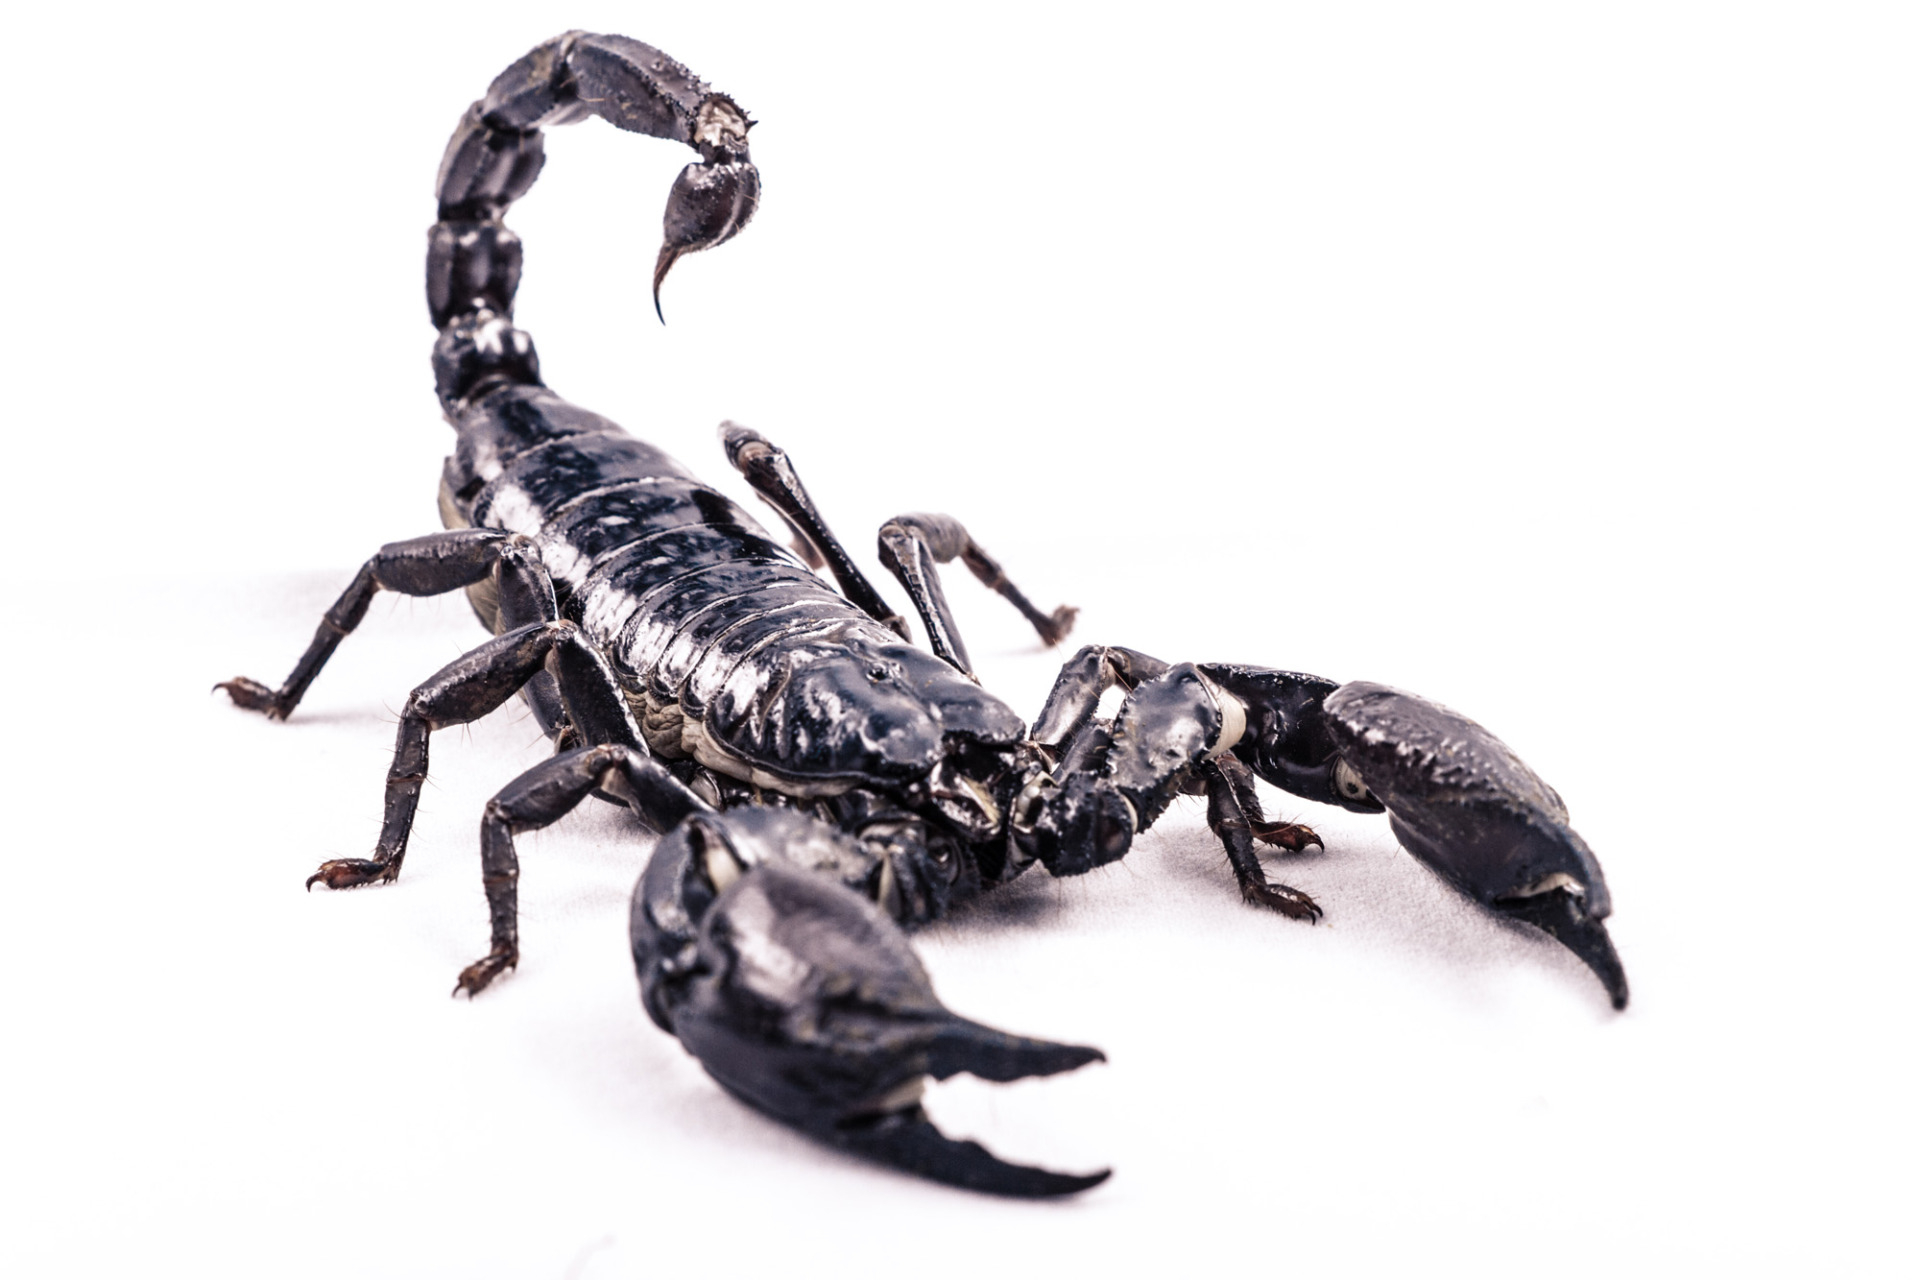
\includegraphics{figures/general/scorpion.jpg}}
    \else
    \fi
}
\newcommand{\newImageResize}[1]{
    \ifIMAGES
        \centering
        \IfFileExists{#1}{
            \resizebox{\textwidth}{!}{
                \includegraphics{#1}
            }
        }
        {
            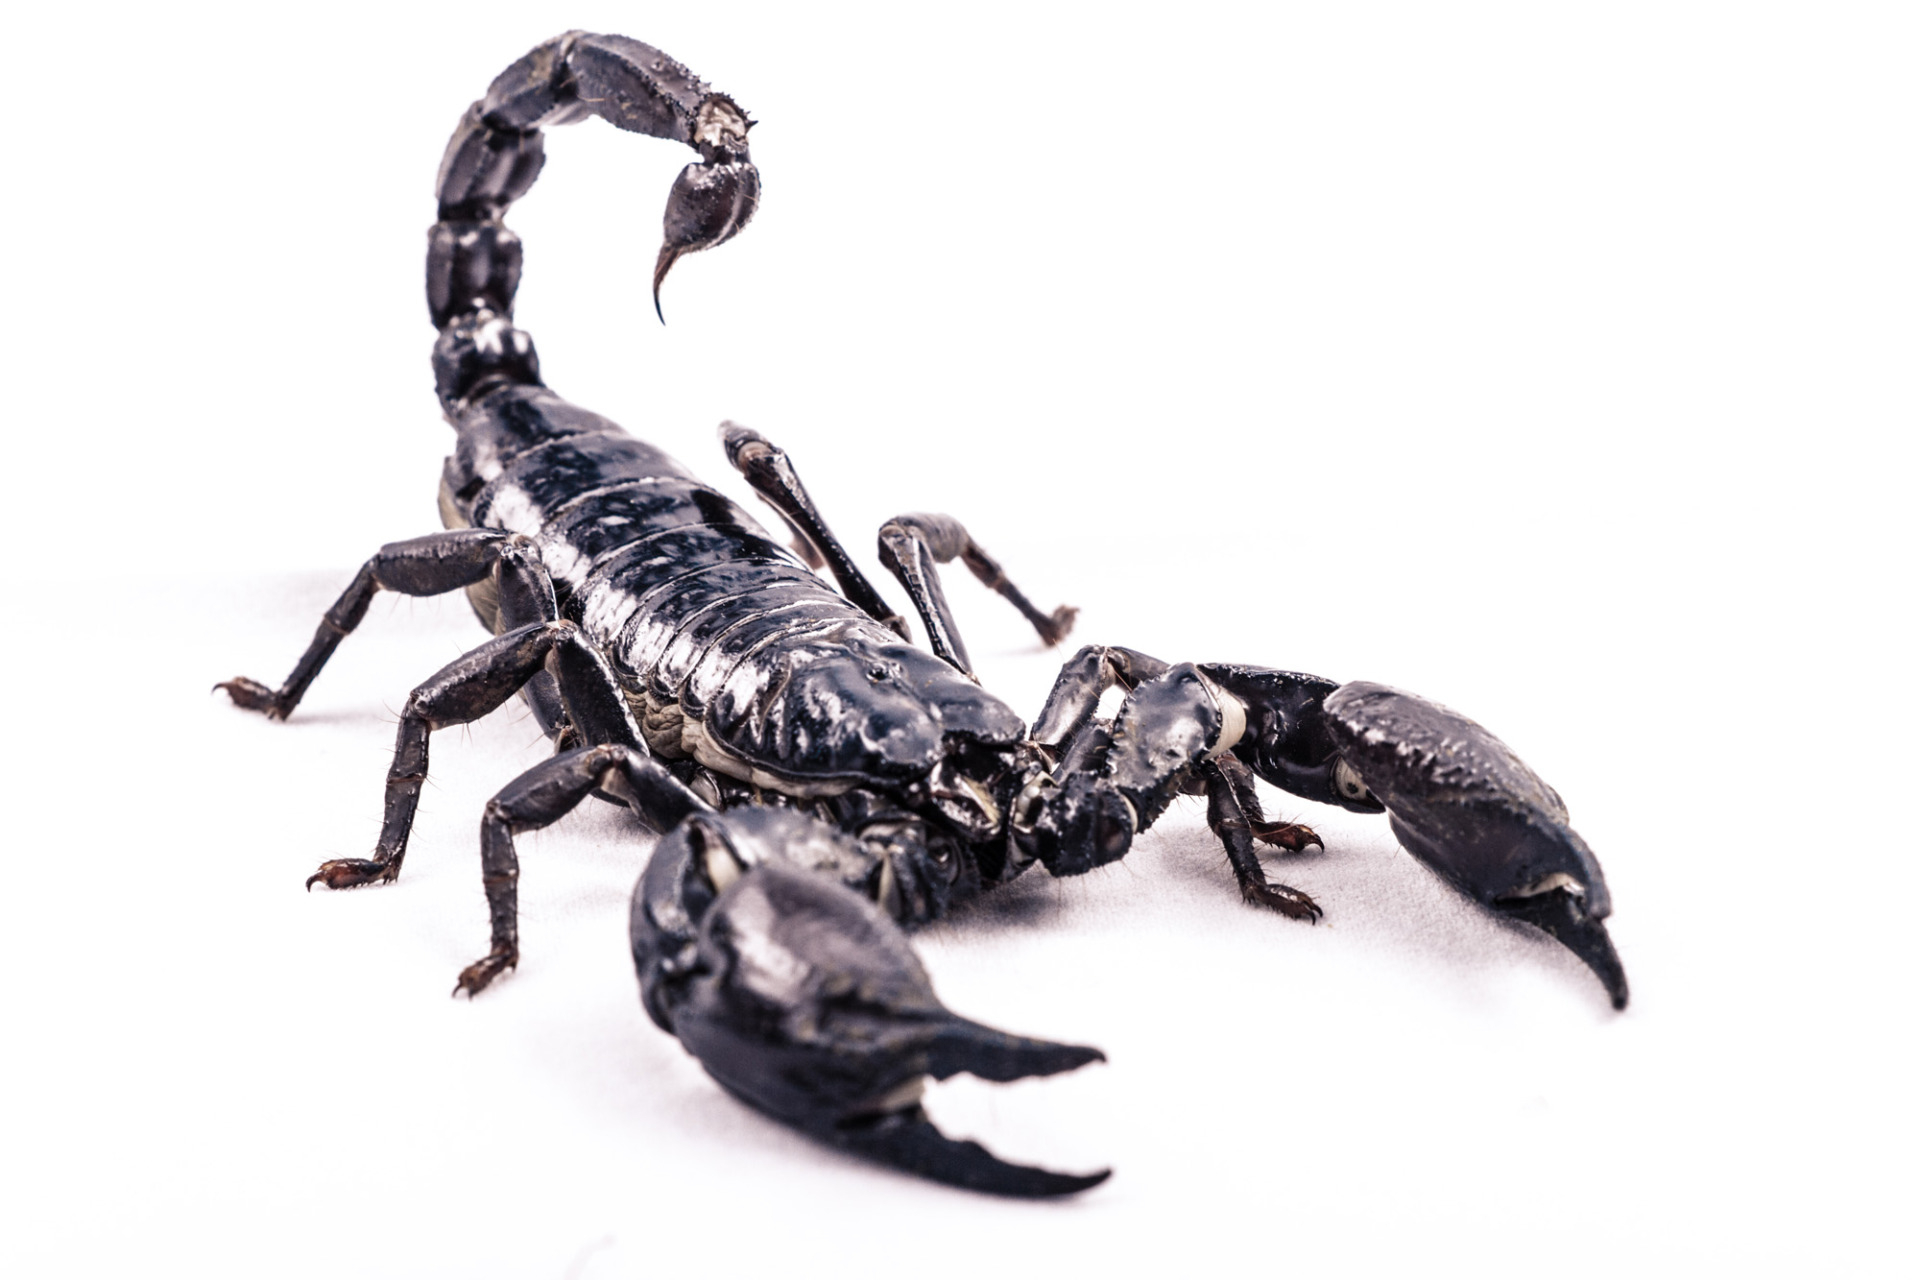
\includegraphics{figures/general/scorpion.jpg}
        }
    \else
    \fi
}
\newcommand{\newImageResizeCustom}[2]{
    \ifIMAGES
        \centering
        \IfFileExists{#2}{
            \resizebox{#1\textwidth}{!}{
                \includegraphics{#2}
            }
        }
        {
            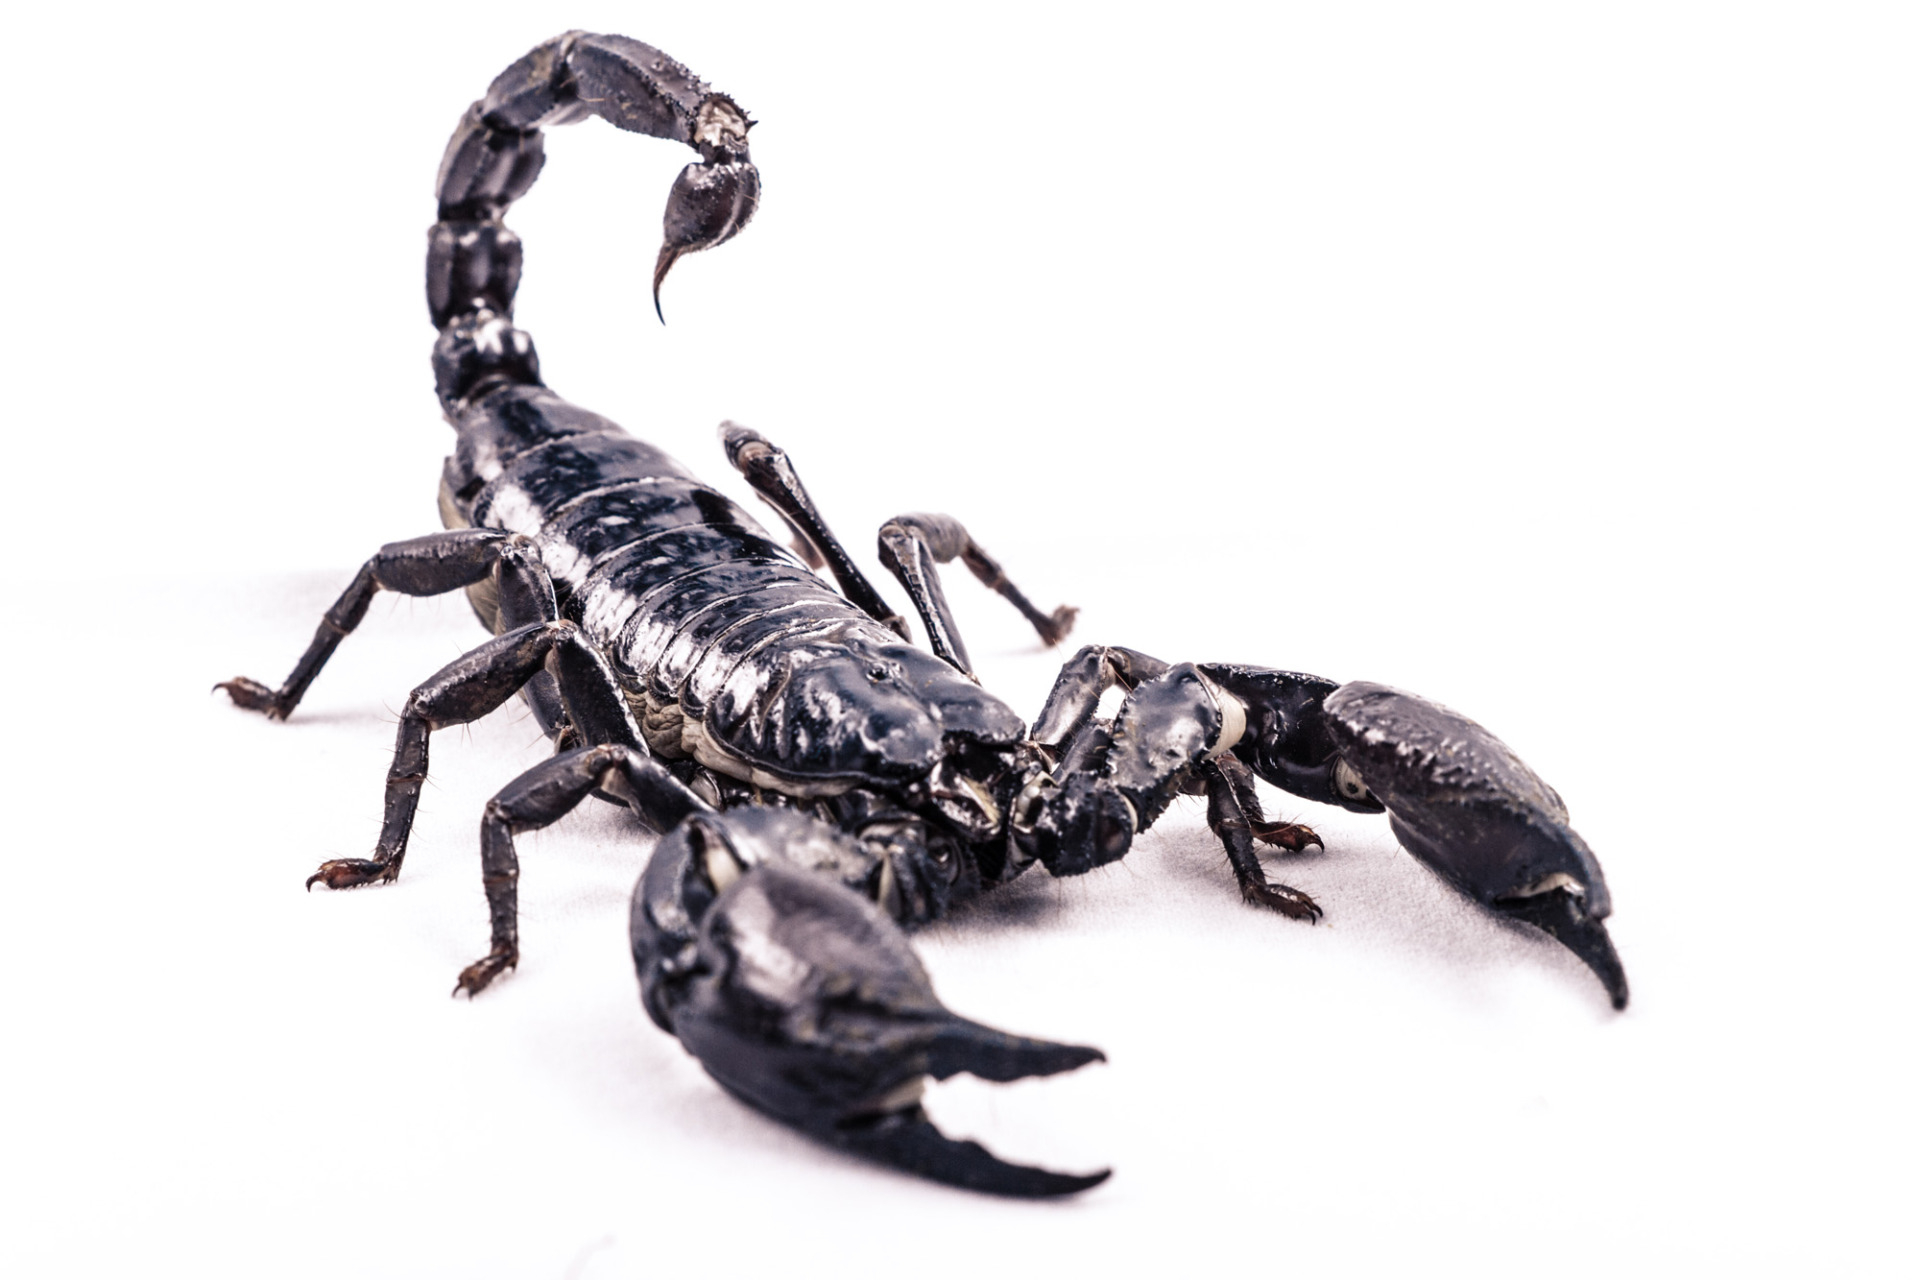
\includegraphics{figures/general/scorpion.jpg}
        }
    \else
    \fi
}
\newcommand{\newImageResizeHalf}[1]{
    \ifIMAGES
        \centering
        \IfFileExists{#1}{
            \resizebox{0.48\textwidth}{!}{
                \includegraphics{#1}
            }
        }
        {
            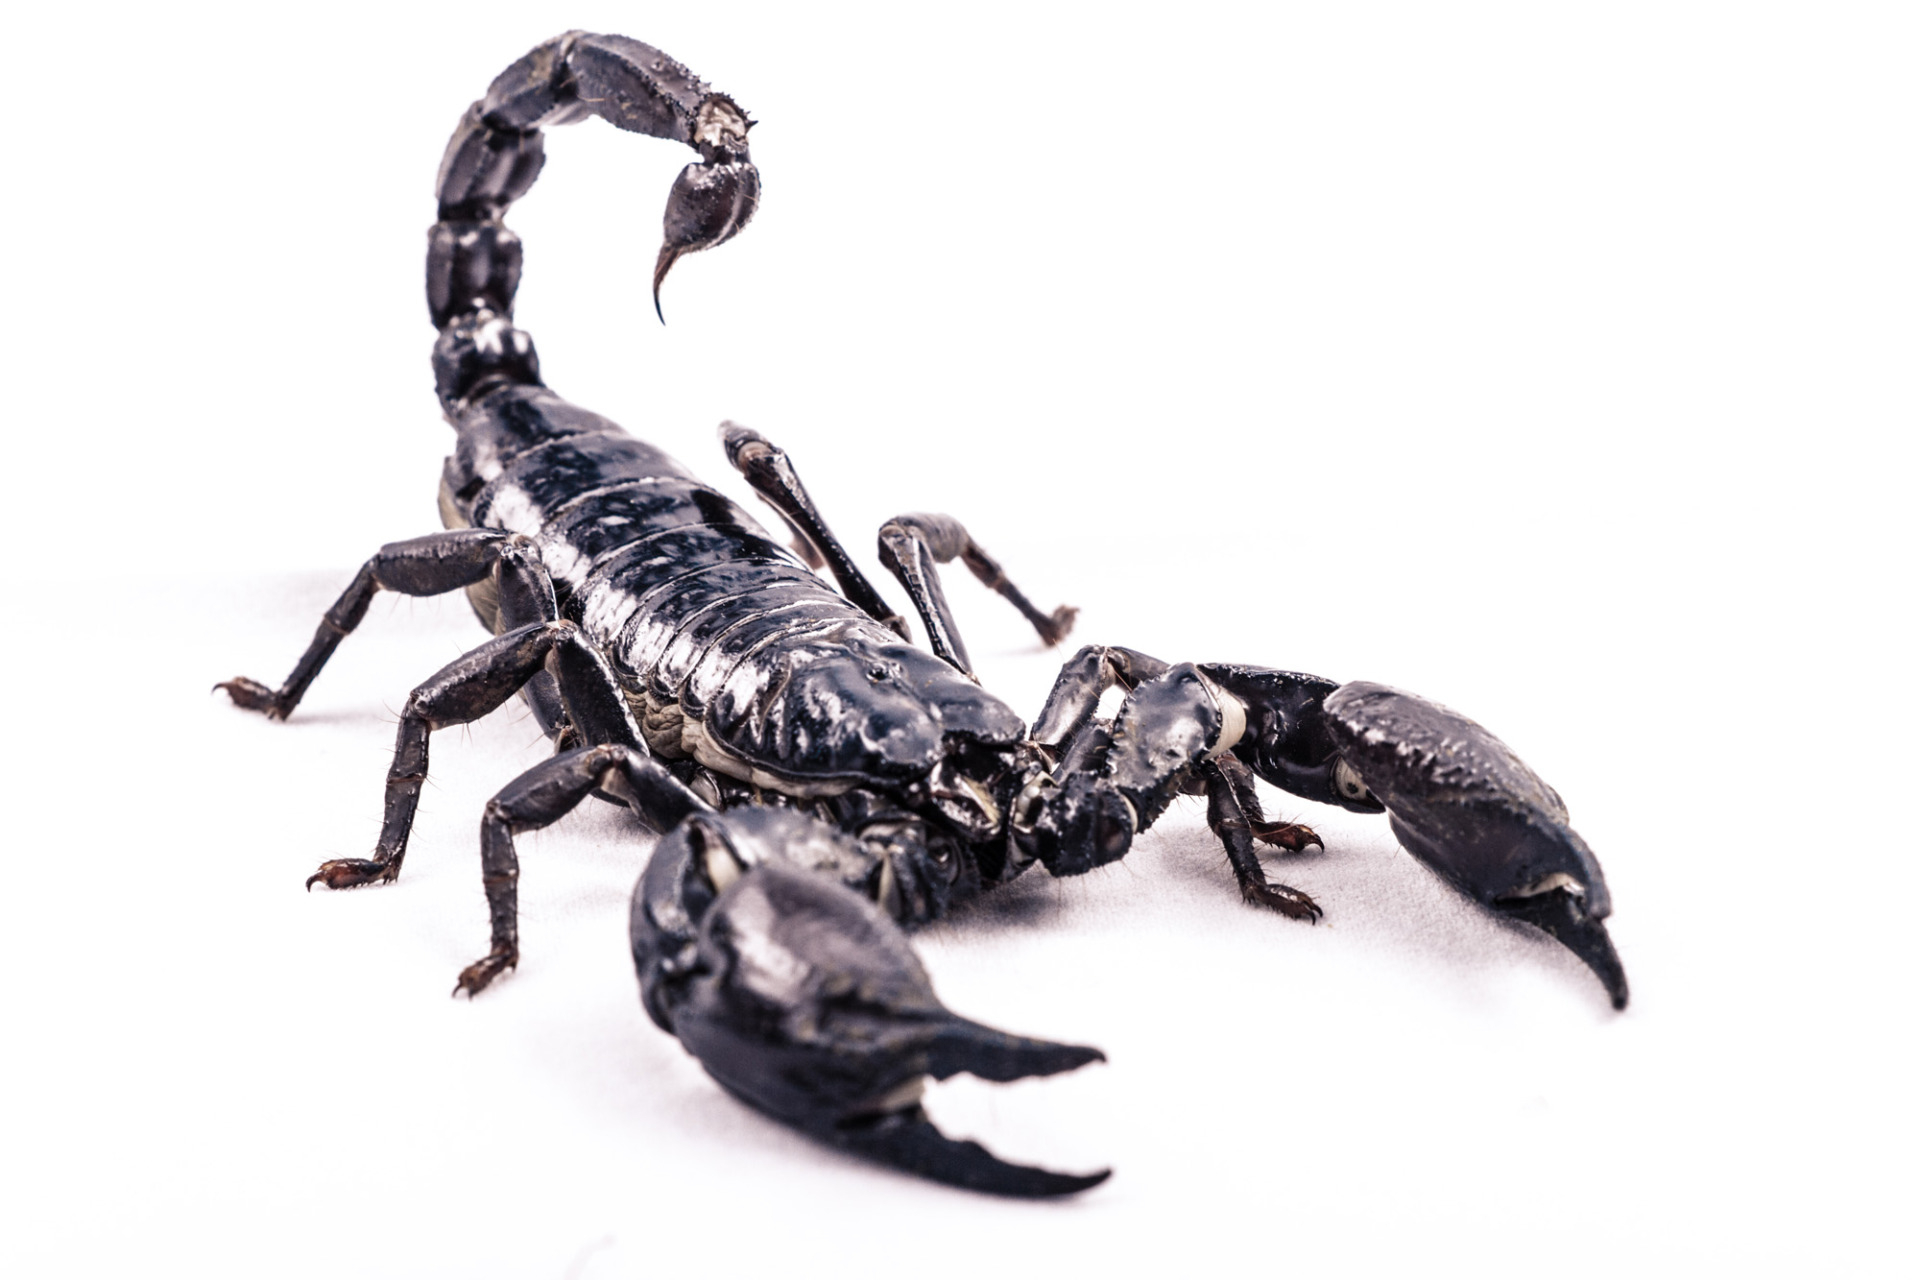
\includegraphics{figures/general/scorpion.jpg}
        }
    \else
    \fi
}
\newcommand{\newImageScale}[2]{
    \ifIMAGES
        \centering
        \IfFileExists{#1}{\includegraphics[scale=#2]{#1}}{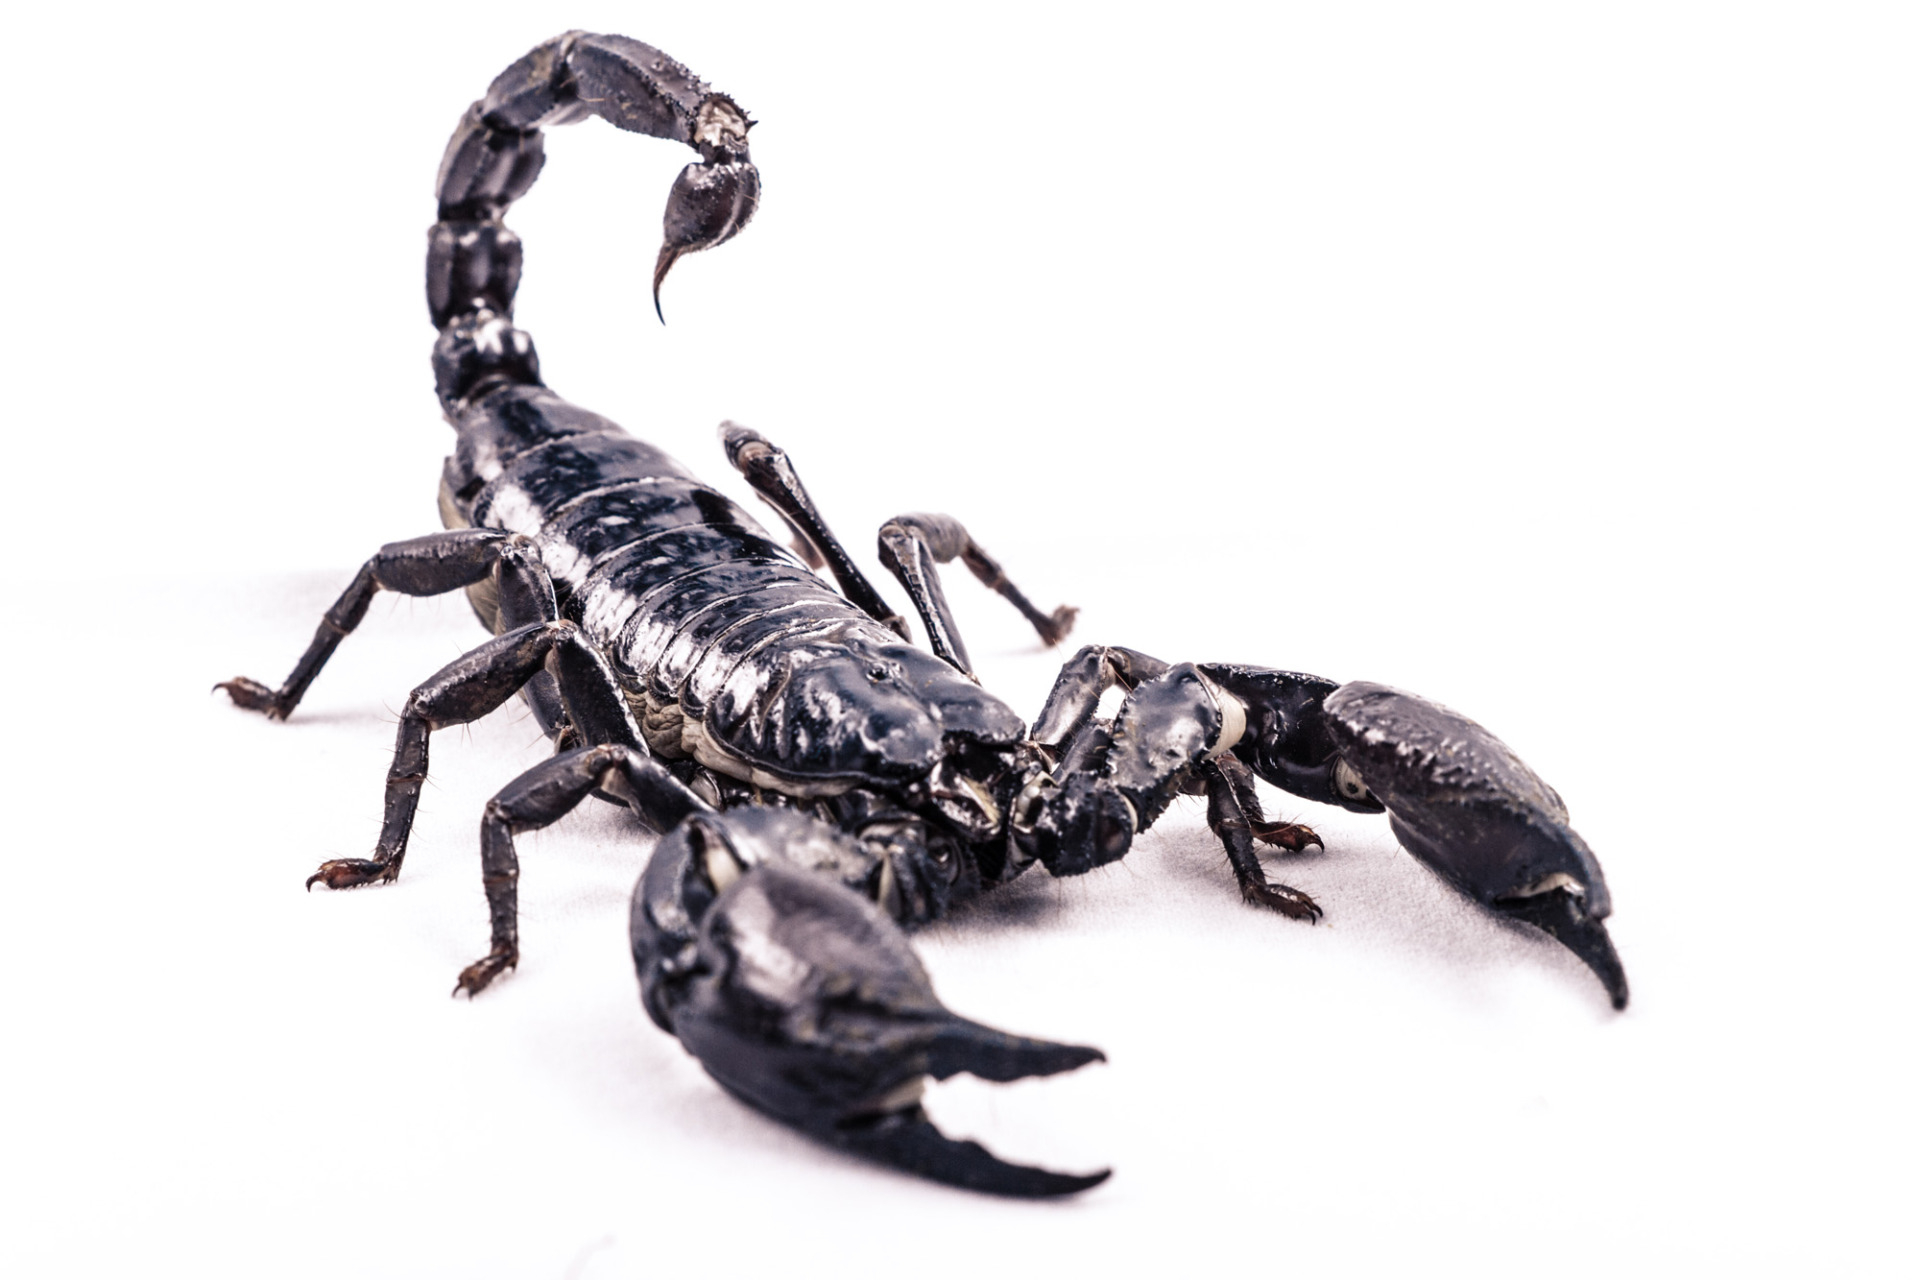
\includegraphics{figures/general/scorpion.jpg}}
    \else
    \fi
}
\newcommand{\newImageScaleRot}[2]{
    \ifIMAGES
        \centering
        \IfFileExists{#1}{\includegraphics[scale=#2,angle=-90]{#1}}{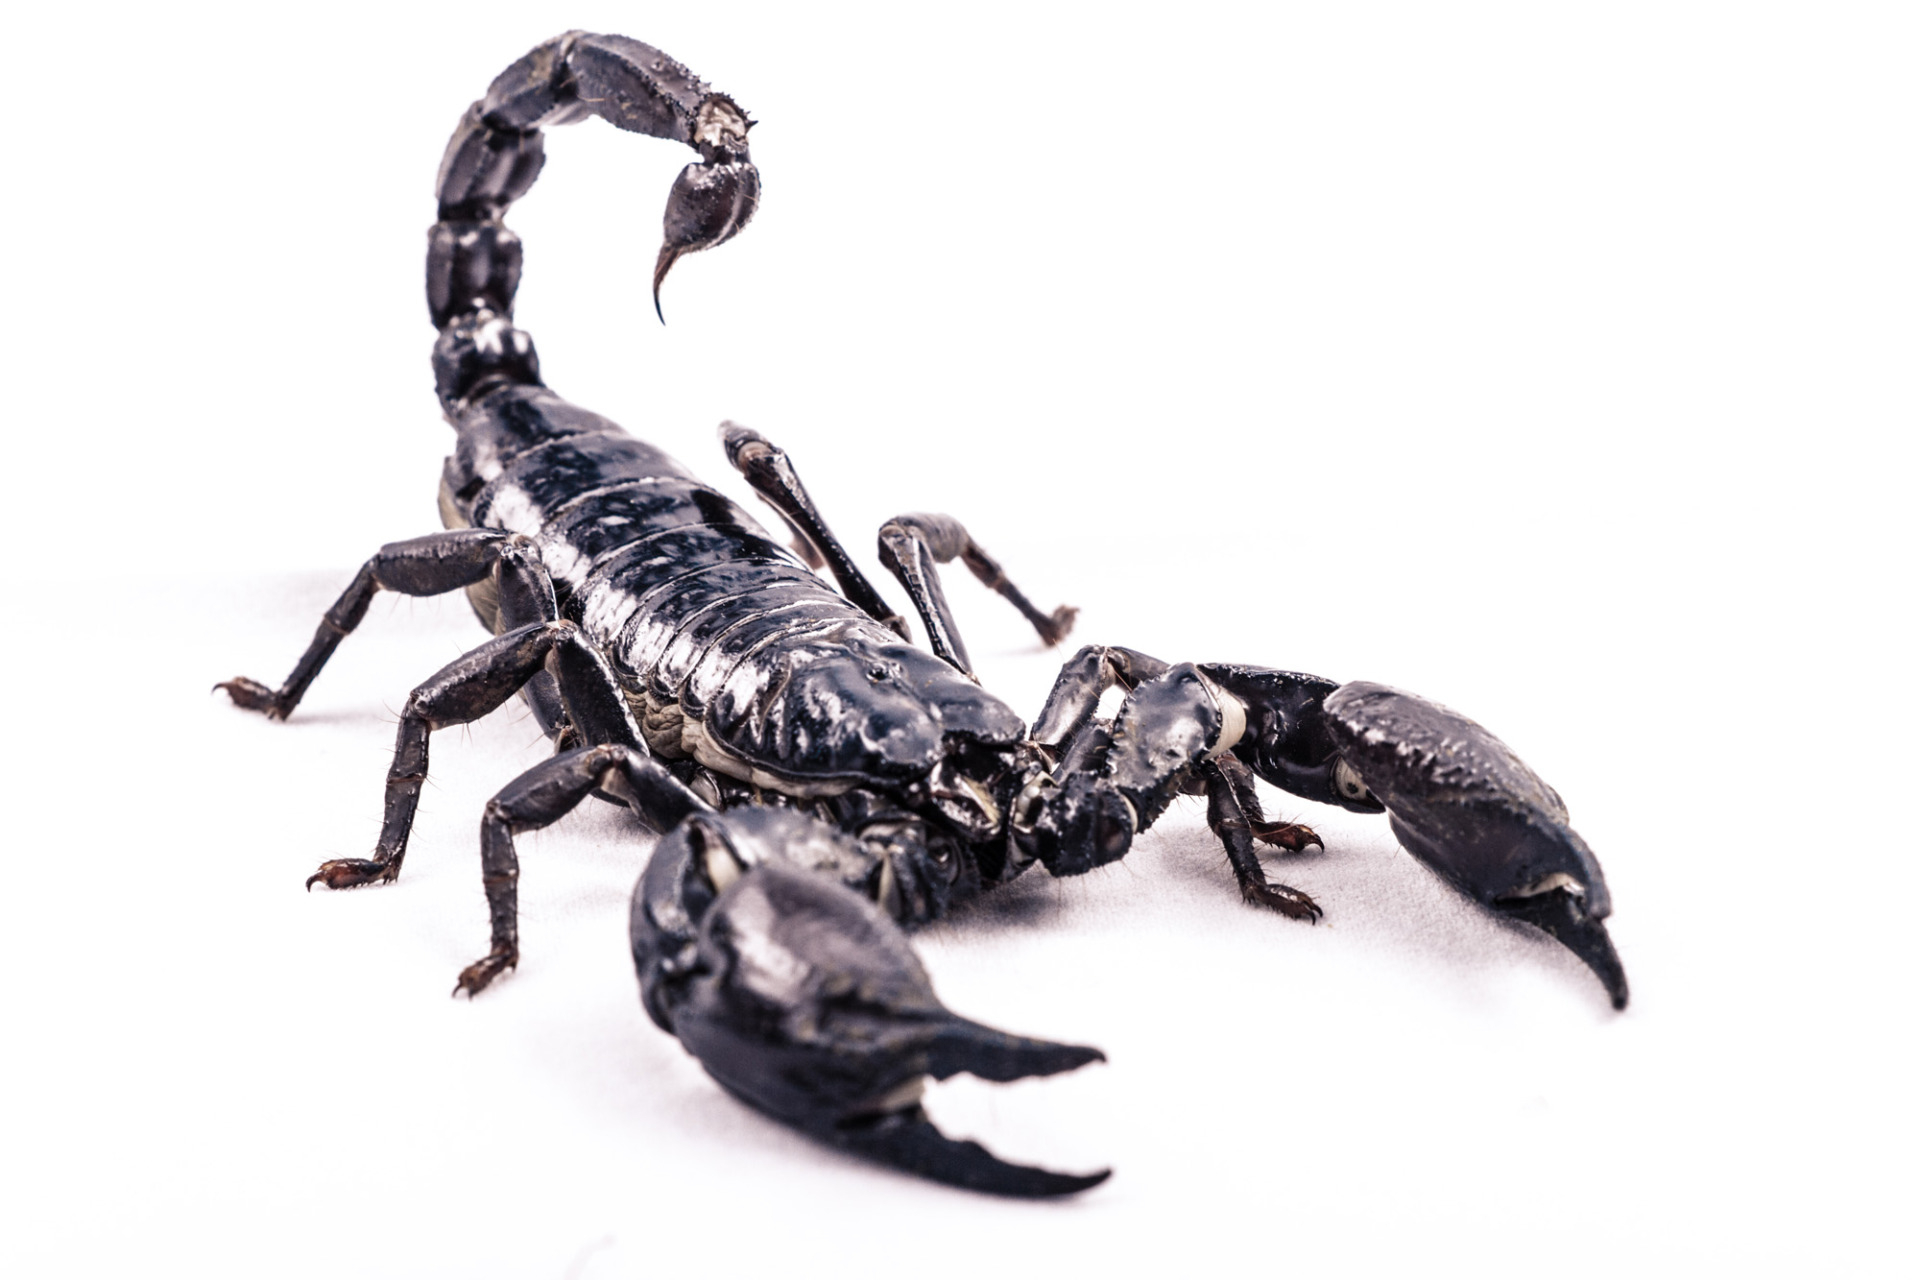
\includegraphics{figures/general/scorpion.jpg}}
    \else
    \fi
}

%---------------------------------------------------
% Equation helpers
\newcommand{\myvec}[1]{\ensuremath{\begin{pmatrix}#1\end{pmatrix}}}

\newcommand{\hl}[1]{{\color{red}#1}}


\newcommand\tenPlots[9]{%
    \def\tempa{#1}%
    \def\tempb{#2}%
    \def\tempc{#3}%
    \def\tempd{#4}%
    \def\tempe{#5}%
    \def\tempf{#6}%
    \def\tempg{#7}%
    \def\temph{#8}%
    \def\tempi{#9}%
    \tenPlotsContinued
}
\newcommand\tenPlotsContinued[3]{%
    %\newcommand{\tenPlots}[12]{
    \begin{figure}[ht]
        \centering
        \subfloat[]{
            \includegraphics[width=0.32\textwidth]{\tempc} \hfill
            \label{\tempb-1}
        }
        \subfloat[]{
            \includegraphics[width=0.32\textwidth]{\tempd} \hfill
            \label{\tempb-2}
        }
        \subfloat[]{
            \includegraphics[width=0.32\textwidth]{\tempd} \hfill
            \label{\tempb-3}
        } \\
        \subfloat[]{
            \includegraphics[width=0.32\textwidth]{\tempf} \hfill
            \label{\tempb-4}
        }
        \subfloat[]{
            \includegraphics[width=0.32\textwidth]{\tempg} \hfill
            \label{\tempb-5}
        }
        \subfloat[]{
            \includegraphics[width=0.32\textwidth]{\temph} \hfill
            \label{\tempb-6}
        } \\
        \subfloat[]{
            \includegraphics[width=0.32\textwidth]{\tempi} \hfill
            \label{\tempb-7}
        }
        \subfloat[]{
            \includegraphics[width=0.32\textwidth]{#1} \hfill
            \label{\tempb-8}
        }
        \subfloat[]{
            \includegraphics[width=0.32\textwidth]{#2} \hfill
            \label{\tempb-9}
        } \\
        \subfloat[]{
            \includegraphics[width=0.32\textwidth]{#3} \hfill
            \label{\tempb-10}
        }
        {\caption{\tempa
                \label{\tempb} }}
    \end{figure}
}

\newcommand\ninePlots[9]{%
    \def\tempa{#1}%
    \def\tempb{#2}%
    \def\tempc{#3}%
    \def\tempd{#4}%
    \def\tempe{#5}%
    \def\tempf{#6}%
    \def\tempg{#7}%
    \def\temph{#8}%
    \def\tempi{#9}%
    \ninePlotsContinued
}
\newcommand\ninePlotsContinued[2]{%
    %\newcommand{\tenPlots}[12]{
    \begin{figure}[ht]
        \centering
        \subfloat[]{
            \includegraphics[width=0.32\textwidth]{\tempc} \hfill
            \label{\tempb-1}
        }
        \subfloat[]{
            \includegraphics[width=0.32\textwidth]{\tempd} \hfill
            \label{\tempb-2}
        }
        \subfloat[]{
            \includegraphics[width=0.32\textwidth]{\tempd} \hfill
            \label{\tempb-3}
        } \\
        \subfloat[]{
            \includegraphics[width=0.32\textwidth]{\tempf} \hfill
            \label{\tempb-4}
        }
        \subfloat[]{
            \includegraphics[width=0.32\textwidth]{\tempg} \hfill
            \label{\tempb-5}
        }
        \subfloat[]{
            \includegraphics[width=0.32\textwidth]{\temph} \hfill
            \label{\tempb-6}
        } \\
        \subfloat[]{
            \includegraphics[width=0.32\textwidth]{\tempi} \hfill
            \label{\tempb-7}
        }
        \subfloat[]{
            \includegraphics[width=0.32\textwidth]{#1} \hfill
            \label{\tempb-8}
        }
        \subfloat[]{
            \includegraphics[width=0.32\textwidth]{#2} \hfill
            \label{\tempb-9}
        } 
        {\caption{\tempa
                \label{\tempb} }}
    \end{figure}
}

\newcommand{\fivePlots}[7]{
    \begin{figure}[ht]
        \centering
        \subfloat[]{
            \includegraphics[width=0.32\textwidth]{#3} \hfill
            \label{#2-1}
        }
        \subfloat[]{
            \includegraphics[width=0.32\textwidth]{#4}
            \label{#2-2}
        }
        \subfloat[]{
            \includegraphics[width=0.32\textwidth]{#5} \hfill
            \label{#2-3}
        } \\
        \subfloat[]{
            \includegraphics[width=0.32\textwidth]{#6} \hfill
            \label{#2-4}
        }
        \subfloat[]{
            \includegraphics[width=0.32\textwidth]{#7} \hfill
            \label{#2-5}
        }
        {\caption{#1
                \label{#2} }}
    \end{figure}
}

\newcommand{\sixPlots}[9]{
    \begin{figure}[t]
        \centering
        \subfloat[]{
            \includegraphics[width=0.32\textwidth]{#3} \hfill
            \label{#2-1}
        }
        \subfloat[]{
            \includegraphics[width=0.32\textwidth]{#4} \hfill
            \label{#2-2}
        }
        \subfloat[]{
            \includegraphics[width=0.32\textwidth]{#5} \hfill
            \label{#2-3}
        } \\
        \subfloat[]{
            \includegraphics[width=0.32\textwidth]{#6} \hfill
            \label{#2-4}
        }
        \subfloat[]{
            \includegraphics[width=0.32\textwidth]{#7} \hfill
            \label{#2-5}
        }
        \subfloat[]{
            \includegraphics[width=0.32\textwidth]{#8} \hfill
            \label{#2-5}
        }
        {\caption[#9]{#1
                \label{#2} }}
    \end{figure}
}

% -----------------------------------------------------------------------
% Short cuts

\newcommand{\myc}[1]{Ref.~\cite{#1}}

\newcommand{\HWW}{\ensuremath{H\rightarrow W^{\pm}W^{\mp^*}}\xspace}
\newcommand{\HWWdet}{\ensuremath{H\,{\rightarrow}\,W^{\pm}W^{\mp^*}\,{\rightarrow}\,\ell^-\bar{\nu} \ell^+\nu}\hspace{0.07em}}
\def\myurl{\hfil\penalty 100 \hfilneg \hbox}
\newcommand{\Zmumu}{\ensuremath{Z \rightarrow \mu\mu}\xspace}
\newcommand{\Jpsimumu}{\ensuremath{J/\psi \rightarrow \mu\mu}\xspace}
\newcommand{\ttH}{\ensuremath{t\bar{t}H}\xspace}

\newcommand{\intLumi}{\ensuremath{L_\text{int}}\xspace}
\newcommand{\instLumi}{\ensuremath{\mathcal{L}}\xspace}
\newcommand{\comEn}{\ensuremath{\sqrt{s}}\xspace}

\newcommand{\ETmiss}{\ensuremath{E_{\text{T}}^{\text{miss}}}\xspace}
\newcommand{\ETmissvec}{\ensuremath{\vec{E}_{\text{T}}^{\text{ miss}}}\xspace}
\newcommand{\pTmiss}{\ensuremath{p_{\text{T}}^{\text{miss}}}\xspace}
\newcommand*{\ETvec}{\ensuremath{\vec{E}_{\text{T}}}\xspace}
\newcommand*{\pTvec}{\ensuremath{\vec{p}_{\text{T}}}\xspace}
\newcommand*{\Ecluster}{\ensuremath{E^{\text{cluster}}}\xspace}
\newcommand*{\Edepavg}{\ensuremath{\left< E_{\text{dep}} \right>}\xspace}
\newcommand*{\ptrack}{\ensuremath{p^{\text{track}}}\xspace}
\newcommand*{\pTtrack}{\ensuremath{p_{\text{T}}^{\text{track}}}\xspace}
\newcommand*{\Eoverpexp}{\ensuremath{\left< E^{\text{cluster}}_{\text{ref}} / p^{\text{track}}_{\text{ref}} \right> }\xspace}

\newcommand{\pTPUsub}{\ensuremath{p_{\text{T}}^{\text{PU subtracted}}}\xspace}
\newcommand{\EPUsub}{\ensuremath{E_{\text{T}}^{\text{PU subtracted}}}\xspace}

\newcommand{\ETmisssimplesign}{\ensuremath{E_{\text{T}}^{\text{miss, simple sign}}}\xspace}
\newcommand{\ETmisssign}{\ensuremath{E_{\text{T}}^{\text{miss, significance}}}\xspace}

\newcommand{\METSigsimple}{\ensuremath{S_{\text{simple}}}\xspace}
\newcommand{\METSigobject}{\ensuremath{S_{\text{object-based}}}\xspace}

\newcommand{\TSTMET}{\ensuremath{\text{TST} E_{\text{T}}^{\text{miss}}}\xspace}
\newcommand{\CSTETmiss}{\ensuremath{\text{CST} E_{\text{T}}^{\text{miss}}}\xspace}

\newcommand{\Npileup}{\ensuremath{N^{\text{pile-up}}}\xspace}
\newcommand{\NpileuppT}{\ensuremath{N^{\text{pile-up}\left(\pT\right)}}\xspace}
\newcommand{\Npileupconstscale}{\ensuremath{N^{\text{pile-up}}_{\text{const scale}}}\xspace}
\newcommand{\Nmuzero}{\ensuremath{N^{\mu=0}}\xspace}
\newcommand{\Nfull}{\ensuremath{N^{\text{full}}}\xspace}
\newcommand{\Rrandomcone}{\ensuremath{R_{\text{RC}}}\xspace}
\newcommand{\RRC}{\ensuremath{R_{\text{RC}}}\xspace}
\newcommand{\sigmaRC}{\ensuremath{\sigma_{\text{RC}}}\xspace}

\newcommand{\pTconeX}{\ensuremath{p_{\text{T}}^{\text{coneX}}}\xspace}
\newcommand{\pTconetwenty}{\ensuremath{p_{\text{T}}^{\text{cone20}}}\xspace}
\newcommand{\pTvarcone}{\ensuremath{p_{\text{T}}^{\text{varcone}}}\xspace}
\newcommand{\ETconeX}{\ensuremath{E_{\text{T}}^{\text{coneX}}}\xspace}
\newcommand{\pTcone}{\ensuremath{p_{\text{T}}^{\text{cone}}}\xspace}
\newcommand{\ETcone}{\ensuremath{E_{\text{T}}^{\text{cone}}}\xspace}
\newcommand{\ETconetwenty}{\ensuremath{E_{\text{T}}^{\text{cone20}}}\xspace}

\newcommand{\pTrandomcone}{\ensuremath{p_{\text{T}}^{\text{Rcone}}}\xspace}

\newcommand{\mT}{\ensuremath{m_{\text T}}\xspace}
\newcommand{\absetadet}{\ensuremath{|\etadet|}\xspace}

\newcommand{\mcjer}{\ensuremath{\sigma_{\text{MCJER}}}\xspace}
\newcommand{\responsejer}{\ensuremath{\sigma_{\text{Response JER}}}\xspace}
\newcommand{\fEM}{\ensuremath{f_{\text{em}}}\xspace}

\newcommand{\Rscan}{\ensuremath{R\text{-scan}}\xspace}

\newcommand{\HWWhalfdet}{\ensuremath{H\,{\rightarrow}\,$~$WW^*\,{\rightarrow}\,$~$\ell\nu\ell\nu}\xspace}
\newcommand*{\ZeroJet}{\ensuremath{N_\text{jet}{=}\,0}\xspace}
\newcommand*{\OneJet}{\ensuremath{N_\text{jet}{=}\,1}\xspace}
\newcommand*{\TwoJet}{\ensuremath{N_\text{jet}{\ge}\,2}\xspace}
%\newcommand{\Ztautau}{\mbox{$Z/\gamma^*\,{\rightarrow}\,\tau\tau$}\,}
\newcommand{\Nbjet}{\ensuremath{N_{\text{$b$-jet}}}}
\newcommand{\Ntrkjet}{\ensuremath{N_{\text{jet}}^{\text{trk jet}}}}
%\newcommand{\Nbjetsub}{\ensuremath{N_{\text{$b$-jet}}}}
\newcommand{\nbJet}{\ensuremath{N_{\text{$b$-jet}}}}
\newcommand{\nbtrkjet}{\ensuremath{N_{\text{$b$-jet}}^{\text{track}}}}
\newcommand{\nbcalojet}{\ensuremath{N_{\text{$b$-jet}}^{\text{calo}}}}
\newcommand{\nbjet}{\ensuremath{N_{\text{$b$-jet}}}}
\newcommand*{\Zpoiss}{\ensuremath{Z_{\text{exp}}^{\text{Poiss}}}}
\newcommand{\Nbjetsub}{\ensuremath{N_{\text{$b$-jet}}^{\pT\,{>}\,20\,\GeV}}}
\newcommand{\Nbjetnom}{\ensuremath{N_{\text{$b$-jet}}^{\pT\,{>}\,30\,\GeV}}}
\newcommand{\Nbjetbetween}{\ensuremath{N_{\text{$b$-jet}}^{20\,\GeV{<}\,\pT\,{<}\,30\,\GeV}}}

\newcommand*{\bcaloveto}{\ensuremath{N^{\pT>20\,\GeV}_{\text{$b$-calo-jet}} = 0}}
\newcommand*{\btrkveto}{\ensuremath{N^{\pT>7\,\GeV, \text{WP77}}_{\text{$b$-track-jet}} = 0}}

\newcommand*{\bcalotag}{\ensuremath{N^{\pT>20\,\GeV)}_{\text{$b$-calo-jet}} \ge 1}}
\newcommand*{\topibcalotag}{\ensuremath{N^{\pT>20\,\GeV)}_{\text{$b$-calo-jet}} = 1}}
\newcommand*{\btrktag}{\ensuremath{N^{\pT>7\,\GeV, \text{WP77}}_{\text{$b$-track-jet}} \ge 1}}
\newcommand*{\topibtrktag}{\ensuremath{N^{\pT>7\,\GeV, \text{WP77}}_{\text{$b$-track-jet}} = 1}}
% Label for alternative working point of 85
\newcommand*{\albtrkveto}{\ensuremath{N^{\pT>7\,\GeV, \text{WP85}}_{\text{$b$-track-jet}} = 0}}
\newcommand*{\albtrktag}{\ensuremath{N^{\pT>7\,\GeV, \text{WP85}}_{\text{$b$-track-jet}} \ge 1}}
\newcommand*{\altopibtrktag}{\ensuremath{N^{\pT>7\,\GeV, \text{WP85}}_{\text{$b$-track-jet}} = 1}}
\newcommand*{\caloandtrkveto}{\ensuremath{N^{\pT>20\,\GeV}_{\text{$b$-calo-jet}} = N^{\pT>7\,\GeV, \text{WP77}}_{\text{$b$-track-jet}} = 0}}
\newcommand*{\caloandaltrkveto}{\ensuremath{N^{\pT>20\,\GeV}_{\text{$b$-calo-jet}} = N^{\pT>7\,\GeV, \text{WP85}}_{\text{$b$-track-jet}} = 0}}
\newcommand*{\caloandtrktag}{\ensuremath{N^{\pT>20\,\GeV}_{\text{$b$-calo-jet}} \ge 1 \,\,\&\,\, N^{\pT>7\,\GeV, \text{WP77}}_{\text{$b$-track-jet}} \ge 1}}
\newcommand*{\caloandaltrktag}{\ensuremath{N^{\pT>20\,\GeV}_{\text{$b$-calo-jet}} \ge 1 \,\,\&\,\, N^{\pT>7\,\GeV, \text{WP85}}_{\text{$b$-track-jet}} \ge 1}}
\newcommand*{\topicaloandtrktag}{\ensuremath{N^{\pT>20\,\GeV}_{\text{$b$-calo-jet}} = 1 \,\,\&\,\, N^{\pT>7\,\GeV, \text{WP77}}_{\text{$b$-track-jet}} \ge 1}}
\newcommand*{\topicaloandaltrktag}{\ensuremath{N^{\pT>20\,\GeV}_{\text{$b$-calo-jet}} = 1 \,\,\&\,\, N^{\pT>7\,\GeV, \text{WP85}}_{\text{$b$-track-jet}} \ge 1}}

\newcommand{\cmark}{\ding{52}}%
\newcommand{\xmark}{\ding{53}}%


\newcommand*{\SRojDFMlliPtSubLeadte}{$N_{\mathrm{jet}}=0,\, m_{\ell\ell}^{10-30},\, p_{\mathrm{T,\ell_2}}^{15-20},\, \mu e$}
\newcommand*{\SRojDFMlliPtSubLeadtm}{$N_{\mathrm{jet}}=0,\, m_{\ell\ell}^{10-30},\, p_{\mathrm{T,\ell_2}}^{15-20},\, e \mu$}
\newcommand*{\SRojDFMlliPtSubLeadthe}{$N_{\mathrm{jet}}=0,\, m_{\ell\ell}^{10-30},\, p_{\mathrm{T,\ell_2}}^{>20},\, \mu e$}
\newcommand*{\SRojDFMlliPtSubLeadthm}{$N_{\mathrm{jet}}=0,\, m_{\ell\ell}^{10-30},\, p_{\mathrm{T,\ell_2}}^{>20},\, e \mu$}
\newcommand*{\SRojDFMlltPtSubLeadte}{$N_{\mathrm{jet}}=0,\, m_{\ell\ell}^{30-55},\, p_{\mathrm{T,\ell_2}}^{15-20},\, \mu e$}
\newcommand*{\SRojDFMlltPtSubLeadtm}{$N_{\mathrm{jet}}=0,\, m_{\ell\ell}^{30-55},\, p_{\mathrm{T,\ell_2}}^{15-20},\, e \mu$}
\newcommand*{\SRojDFMlltPtSubLeadthe}{$N_{\mathrm{jet}}=0,\, m_{\ell\ell}^{30-55},\, p_{\mathrm{T,\ell_2}}^{>20},\, \mu e$}
\newcommand*{\SRojDFMlltPtSubLeadthm}{$N_{\mathrm{jet}}=0,\, m_{\ell\ell}^{30-55},\, p_{\mathrm{T,\ell_2}}^{>20},\, e \mu$}

\newcommand*{\SRijDFMlliPtSubLeadte}{$N_{\mathrm{jet}}=1,\, m_{\ell\ell}^{10-30},\, p_{\mathrm{T,\ell_2}}^{15-20},\, \mu e$}
\newcommand*{\SRijDFMlliPtSubLeadtm}{$N_{\mathrm{jet}}=1,\, m_{\ell\ell}^{10-30},\, p_{\mathrm{T,\ell_2}}^{15-20},\, e \mu$}
\newcommand*{\SRijDFMlliPtSubLeadthe}{$N_{\mathrm{jet}}=1,\, m_{\ell\ell}^{10-30},\, p_{\mathrm{T,\ell_2}}^{>20},\, \mu e$}
\newcommand*{\SRijDFMlliPtSubLeadthm}{$N_{\mathrm{jet}}=1,\, m_{\ell\ell}^{10-30},\, p_{\mathrm{T,\ell_2}}^{>20},\, e \mu$}
\newcommand*{\SRijDFMlltPtSubLeadte}{$N_{\mathrm{jet}}=1,\, m_{\ell\ell}^{30-55},\, p_{\mathrm{T,\ell_2}}^{15-20},\, \mu e$}
\newcommand*{\SRijDFMlltPtSubLeadtm}{$N_{\mathrm{jet}}=1,\, m_{\ell\ell}^{30-55},\, p_{\mathrm{T,\ell_2}}^{15-20},\, e \mu$}
\newcommand*{\SRijDFMlltPtSubLeadthe}{$N_{\mathrm{jet}}=1,\, m_{\ell\ell}^{30-55},\, p_{\mathrm{T,\ell_2}}^{>20},\, \mu e$}
\newcommand*{\SRijDFMlltPtSubLeadthm}{$N_{\mathrm{jet}}=1,\, m_{\ell\ell}^{30-55},\, p_{\mathrm{T,\ell_2}}^{>20},\, e \mu$}

\newcommand*{\CRojDFtop}{\ZeroJet\ top control region}
\newcommand*{\CRojDFWW}{\ZeroJet\ $WW$\ control region}
\newcommand*{\CRojDFZtt}{\ZeroJet\ \Ztautau\ control region}
\newcommand*{\CRijDFtop}{\OneJet\ top control region}
\newcommand*{\CRijDFWW}{\OneJet\ $WW$\ control region}
\newcommand*{\CRijDFZtt}{\OneJet\ \Ztautau\ control region}

\newcommand*{\MlliPtSubLeadte}{$m_{\ell\ell}^{10-30},\, p_{\mathrm{T,\ell_2}}^{15-20},\, \mu e$}
\newcommand*{\MlliPtSubLeadtm}{$m_{\ell\ell}^{10-30},\, p_{\mathrm{T,\ell_2}}^{15-20},\, e \mu$}
\newcommand*{\MlliPtSubLeadthe}{$m_{\ell\ell}^{10-30},\, p_{\mathrm{T,\ell_2}}^{>20},\, \mu e$}
\newcommand*{\MlliPtSubLeadthm}{$m_{\ell\ell}^{10-30},\, p_{\mathrm{T,\ell_2}}^{>20},\, e \mu$}
\newcommand*{\MlltPtSubLeadte}{$m_{\ell\ell}^{30-55},\, p_{\mathrm{T,\ell_2}}^{15-20},\, \mu e$}
\newcommand*{\MlltPtSubLeadtm}{$m_{\ell\ell}^{30-55},\, p_{\mathrm{T,\ell_2}}^{15-20},\, e \mu$}
\newcommand*{\MlltPtSubLeadthe}{$m_{\ell\ell}^{30-55},\, p_{\mathrm{T,\ell_2}}^{>20},\, \mu e$}
\newcommand*{\MlltPtSubLeadthm}{$m_{\ell\ell}^{30-55},\, p_{\mathrm{T,\ell_2}}^{>20},\, e \mu$}


\newcommand*{\electronicnoise}{\ensuremath{\sigma_{\text{noise}}^{\text{electronic}}}\xspace}
\newcommand*{\pileupnoise}{\ensuremath{\sigma_{\text{noise}}^{\text{pileup}}}\xspace}


\author{Benjamin Jäger}
\date{\today}
\title{Thesis Outline and Main Results - v0.2}



%-------------------------------------------------------------------------------
% Content
%-------------------------------------------------------------------------------
\begin{document}

\maketitle




\tableofcontents

% List of to-do notes.
%\listoftodos

\newcommand{\chapterdir}{chapters}
%\addchap*{About This Version}
This version of my thesis shows an outline of the content I intend to include and is meant to be reviewed by the committee.
I included a short paragraph stating my main research contributions below.
The figures that will be the main highlights of this thesis are also included:

\begin{itemize}
    \item My work for the jet/etmiss group culminated in the noise term results shown in \cref{fig:noise-term-results-pflow}, which was input to the JER combination, as shown in \cref{fig:jer-combination-incl-noise-term,fig:jer-combination-results,fig:jer-combination-uncertainties}.
    \item My main research focused on the \HWW analysis. The currently public results are shown in \cref{fig:post-fit-final-discriminatns,fig:avocado-plot,fig:stxs-pois-bar-plot,tab:stxs-xsec-uncertainties} (Note: these results will be updated to the ones included in the upcoming paper).
\end{itemize}


% -------------------------------------------------------------------------------
\chapter{Introduction}
\label{chap:introduction}

%\TDinote{}{Maybe want to use Cambria font}
%\hl{Thesis Introduction To Come}
\TDinote{}{Proper Thesis Introduction To Come}


The urge to continuously learn about the world seems deeply rooted in humanity.
%As children we explore our neighborhood, as adults we learn about different professions and cultures, and as we grow older we learn about the lives of the younger generation. 
The field of \emph{particle physics} has taken on the challenge of learning about the fundamental laws of nature. 
In this quest, the Standard Model of particle physics (SM) provides the best theory to date describing the behavior of all known fundamental particles. 
The SM includes three of the four fundamental forces of nature and has been extremely successful in predicting and describing correctly various experimental measurements. 
The culmination of this success was the discovery of a new particle by the ATLAS and CMS collaborations in 2012~\cite{HIGG-2012-27,CMS-HIG-12-028}.
To date, ten years after this discovery, all experimental measurements show consistency of the observed particle with the properties of the long sought-after Higgs boson predicted by the SM almost 50 years earlier.
%Despite this success, however, the SM cannot explain several observable phenomena, such as the asymmetry of matter and antimatter in the universe, and much remains to be understood about the nature of the Higgs boson.
Despite this success, however, the SM cannot explain several observable phenomena, such as the asymmetry between matter and antimatter in the universe, and theoretical puzzles prevail, such as the unification of the SM and Einstein's theory of gravity.
Many of the open questions can be directly linked to the Higgs boson, whose exact nature remains to be understood: Is the Higgs boson a fundamental particle? Why is the mass of the Higgs boson so small? Are there more particles similar to the Higgs boson? 
% Theories beyond the SM that attempt to address these shortcomings include two major implications: First, they posit the existence of new fundamental particles, which motivates the direct search for experimental signatures of these particles; and second, they predict changes in the Higgs boson phenomenology predicted by the SM, which makes the precise study of the Higgs boson one of the most promising research directions. The latter is particularly interesting since no direct discovery of new particles has been made in recent years. 
Many theories beyond the SM that attempt to address these shortcomings have two main implications: First, they posit the existence of new fundamental particles, and second, they predict changes in the Higgs boson phenomenology predicted by the SM. The latter is one of the most promising research directions, in particular, since no direct discovery of new particles has been made in recent years. 
Specifically, the precise measurement of the Higgs boson's couplings to other fundamental particles is crucial to constrain theories beyond the SM and may also reveal possible deviations from the SM predictions, thereby indirectly paving the way to new, undiscovered phenomena. 

% Especially since no direct discovery of new particles has been made in recent years, the precise study of the Higgs boson becomes crucial, as it may reveal possible deviations from the SM that could indirectly pave the way to new, undiscovered phenomena. 
%The main goal of experimental particle physics is to probe these theories to pave the way to a more complete understanding of nature.
%Despite this success, however, there are several questions the SM cannot answer, and much remains to be understood about the nature of the Higgs boson.
% Especially since no direct discovery of new particles has been made in recent years, the study of the Higgs boson is among the most promising research directions.
% In particular, the precise measurement of the interactions of the Higgs boson with all other fundamental particles becomes crucial. 
% This helps to constrain theories beyond the SM, and may also reveal possible deviations from the SM predictions that could pave the way to new, undiscovered phenomena. 
% This allows theories beyond the SM to be constrained and allows potential deviations from the SM predictions to be measured, possibly paving the way to new, undiscovered phenomena. 

The properties of the Higgs boson can be studied in high energy particle collider experiments. 
The only collider that is currently able to produce enough Higgs bosons for study is the Large Hadron Collider (LHC), colliding protons at center-of-mass energies of up to $\sqrt{s} = 13\,$TeV. 
%\footnote{Even higher energies are planned for the next operating cycle of the LHC, which will begin at the turn of 2022 and 2023.}
The outcome of the proton-proton ($pp$) collision events are measured with large detector facilities built around the interaction points. 
The ATLAS experiment is one such detector, designed as a multipurpose detector but particularly well-suited to measuring the kind of detector signals that Higgs bosons generate after being produced in the $pp$ collisions.

The Higgs boson decays almost instantaneously after being produced. Hence, only its decay products can be measured in the detector. Since the Higgs boson couples to all massive particles, it can be produced in various production processes and has multiple possible decay modes, which leads to a rich phenomenology of Higgs boson physics. 

This thesis presents cross-section measurements of Higgs boson production in its decay to a pair of $W$ bosons.
The analysis of \HWW\ decays enables some of the most sensitive measurements of Higgs boson processes at the LHC, as it is the second most likely decay mode of the Higgs boson, and provides an excellent control over other types of $pp$ collision events considered as backgrounds. The latter is ensured by selecting events with two leptons in the final state to target \HWWdet decays with leptonically decaying $W$ bosons.
The measurements presented analyze the gluon fusion (ggF) and vector boson fusion (VBF) production mode of the Higgs boson, measuring their cross sections inclusively as well as differentially in various kinematic regions.
The VBF, \HWWdet process (\emph{VBF signal}), in particular, enables the most sensitive measurements of the coupling strength of the Higgs boson to vector bosons at the LHC. 
% . In addition, leptons originating from the $W$ boson decays provide an excellent control over other types of $pp$ collision events considered as backgrounds.
% For this reason, the analysis of \HWWdet decays enables some of the most sensitive measurements of Higgs boson production at the LHC.
The analysis presented is conducted with $pp$ collision data recorded during the second period of data taking at the LHC between 2015 and 2018, known as \RunTwo. The dataset corresponds to an integrated luminosity of 139\,\ifb and was recorded at a center-of-mass energy of $\sqrt{s} = 13\,$TeV.
%The ggF and VBF production cross sections are measured inclusively as well as differentially in various kinematic regions, using the framework of Simplified Template Cross Sections. 
The measurements are performed in a way that allows them to be combined with measurements of other Higgs boson processes to ultimately provide the most precise measurements.
%for example, measurements of $H \to ZZ$ and $H \to \gamma\gamma$ decays. 
%Combined measurements like these 
% Furthermore, the Higgs boson measurements are used as baseline for theory-agnostic interpretations of the data for example in the framework of Effective Field Theories.

The success of the \HWWdet analysis is determined by two main factors: 
First, the ability to precisely estimate the expected number of events given a set of event selection criteria; and second, the ability to distinguish collision events with interesting Higgs boson events from other types of events.
In this thesis, studies are presented that work towards both of these goals.
A contribution to the first task is made by measuring the energy resolution of jets as precisely as possible, which allows selecting Higgs boson events more accurately and reduces measurement uncertainties.
The second challenge is addressed in the analysis of the VBF signal that is difficult to distinguish from non-VBF signal events. 
A supervised machine learning algorithm is used to develop a deep neural network that recognizes patterns of the VBF signal to distinguish it from the backgrounds.
% One may argue, by teaching machines how to learn, humans are able to learn more about the fundamental laws of nature. 
%These patterns are too complex and multidimensional for simple analysis strategies to be efficient, so machines are taught to learn them for us.
%separate Higgs events from backgrounds events. 
This contributes significantly to achieving more precise measurements of Higgs boson processes and thus to making progress in learning about the world around us. 

% 1. Epic Intro
% - The drive to learn seems deeply rooted into humanity. 
% - Learning sits at the core of humanity. 
%  Learning the fundamental laws of nature is the challenge elementary particle physics has set itself up for. 
% The quest for learning how nature behaves is driven by curiosity only. 

% 2. Particle physics / SM
% The current best theory to describe the behavior of the fundamental building blocks of matter, called elementary particles, is known as the Standard Model. 
% It has been hugely successful in describing various experimental measurements correctly. 
% The Higgs boson discovery in 2012 can be regarded as the culmination of success the success story. 
% It updated the status of particle physics as a whole and largely influences future research directions. 
% There open problems and much remains to be understood!

% 3. Higgs takes special place
% The Higgs boson sits at the core of the theory, being connected to 10 out of the 19 free parameters that need to be determined by experimental data.  
% This makes it very important to understand all aspects of Higgs boson physics precisely. In particular, the probability of the Higgs boson to be produced, measured in terms of cross sections, or the interactions with other particles.
% A comprehensive study of the Higgs boson and all its interactions with other particles is therefore essential. 

% 4. Experiments (LHC,  ATLAS)
% Large particle colliders allow testing SM predictions and looking for new phenomena. 
% ATLAS detector

% 5. Analysis 
% This thesis presents a measurement of Higgs production cross sections in its decay to a pair of $W$ bosons. 
% The HWW decay is the second most likely one and provides an excellent opportunity to study the kinematics of specifically the gluon fusion as well as the vector boson fusion production mode of the Higgs boson.

% The success of most physics analyses is determined by two main factors: 
% (i) 
% - the ability to cleverly select collision events so the amount of signal events that are to be measured is large compared to the other ``background'' events.  
% - The ability to distinguish interesting Higgs boson signal events from other types of events.
% (ii) the ability to precisely estimate the expected contributions given the selection criteria (query), with as little uncertainty as possible.

% 6. JER and Higgs cross sections
% For the latter, this thesis presents a measurement of the noise term of the jet energy resolution, allowing to select and disentangle events at a finer resolution. 
% For the former, this thesis presents the development of a deep neural network that discriminates Higgs boson events produced via vector boson fusion. A supervised learning algorithm is used for a neural net to learn to recognize patterns from labelled example data and separate Higgs events from backgrounds events. These patterns are too complex and multidimensional for a human to find, so machines are taught to learn them for us. 
% This allows measuring the amount of VBF, HWW events produced at unprecedented precision. 

% 7. deviations, STXS, further interpretations. 
% The precision measurements of HWW decays can be used for further combinations and interpretations. 





% Learning From Experience: Measurement of HWW decays to two W bosons with a "learned" discriminator

% The Standard Model (SM) of particle physics is currently the most comprehensive theoretical basis for the study of the fundamental laws of nature.

% - To produce collision events at the highest energies, circular accelerators are built in order to gradually increase the energy of the particles.

% \Minote{}{Mention previous experiments? Tevatron, ...other?}

% The ATLAS experiment is operated by one of the world's largest scientific collaborations. A community of about 3000 scientific authors from 181 institutions and 41 countries~\cite{AtlasCollab} work towards making the most precise measurements of the Standard Model and potentially finding experimental hints for New Physics with the ATLAS detector.

% All experimental measurements show remarkable consistency with the predictions of the SM. 

%Only with a precise knowledge of Higgs processes and an understanding of what exact role the Higgs boson plays in nature, fundamental physics can come closer to answering some of the open fundamental questions.  

% By now the Higgs is firmly established in the SM. 

% This might be good for the thesis introduction and is also repeated below
% Physics beyond the SM is typically referred to as ``New Physics''.
% The quest to find new physics is usually driven by looking for deviations of the SM predictions.
% Therefore, it is important to understand with high precision the physics of the SM itself, in particular the properties of the particles that are predicted to couple to new physics. 
% The Higgs boson is often seen as a portal to new physics, which motivates measuring its properties precisely. 

% From current limitations of SM
% The Higgs boson takes a special role in the SM because it is the only fundamental scalar. Its nature makes it a suitable candidate in many models beyond the SM to predict couplings between the Higgs boson and particles from new physics~\cite{2019BHeinemann}.
% This highly motivates precision measurements of the Higgs boson to be able to detect small deviations from the SM predictions. 




% Simulated $pp$ collision events are therefore generated to compare the data against what is expected given the current knowledge of particle physics.

% RESOURCES:
% https://www.nature.com/articles/s41567-020-01054-6.pdf

% From gianotti
% The Higgs boson as a starting point
% Recent experimental results, in particular
% from the LHC, have radically transformed
% the status of particle physics and form
% the basis for future research directions.
% The discovery of the Higgs boson has
% been a turning point, unveiling a particle
% with unprecedented characteristics and
% shedding new light on a phenomenon
% that has surprising similarities with 
% the way certain materials behave
% as superconductors below a critical
% temperature.
% It was fascinating to realize that the same
% phenomenon operates at cosmic scales,
% and made the early Universe undergo
% a phase transition that transformed the
% nature of empty space. Nevertheless,
% believing that the Higgs boson discovery
% has completed our understanding of this
% complex phenomenon is too simplistic.
% On the contrary, much remains to be
% understood about this very special particle,
% including whether it is an elementary
% or composite object, how it leads to the
% peculiar pattern of quark and lepton masses
% observed, what determines the stability of
% the vacuum and what triggered the phase
% transition in the early Universe.
% These questions are still largely
% unexplored experimentally and raise deep
% conceptual concerns theoretically. That is
% why the ESPP update has identified the
% detailed study of the Higgs boson as the
% most pressing priority for the field. Since
% the Higgs boson discovery in 2012 the
% general-purpose LHC experiments, ATLAS
% and CMS, have made extraordinary
% progress in pinning down the features
% of this particle and, by the end of LHC
% operation in 2038 — thanks to the
% high-luminosity upgrades of the collider
% and the detectors — they should be able to
% measure the Higgs boson properties with
% greatly improved precision.
% To gain even deeper insights into the
% Higgs boson and its role in fundamental
% physics, the ESPP recommends an electron–
% positron collider as the next facility, followed
% by a high-energy proton–proton collider in
% the longer term.

% NIMA on 100 TeV collider
% https://arxiv.org/abs/1511.06495



% Precise understanding of Higgs processes may also reveal other deviations from the SM predictions that could, for example, shed light on the matter-antimatter asymmetry of the universe. \todo{FIND citation or leave out!}

\section*{Outline of the thesis and contributions by the author}
This thesis presents research that has been conducted with the ATLAS collaboration. 
The different chapters as well as the level of detail reflect the author's contributions to the research.
The following provides an outline of the thesis including a summary of the author's contributions.

\Cref{chap:theory} summarizes the theoretical framework of the Standard Model and introduces the concepts required to describe and measure proton-proton collision events. 
% \Cref{chap:higgs} introduces all relevant aspects of Higgs boson physics. First, the importance of Higgs boson measurements is highlighted, followed by a description of the phenomenology of Higgs boson processes and the current experimental status.

\Cref{chap:higgs} provides motivation for performing Higgs boson measurements and summarizes the phenomenology and recent measurements of Higgs boson processes. This allows placing the research presented in this thesis in a broader context. 

\Cref{chap:experiment} presents the experimental setup used to measure Higgs boson events, first describing the LHC and then detailing the various detector systems of the ATLAS experiment.

\Cref{chap:objects} discusses the various algorithms that are used in the ATLAS collaboration to reconstruct and identify physics objects. 

\Cref{chap:calibration} discusses how the energy of jets is calibrated with the ATLAS experiment, focusing on the measurement of the noise term of the jet energy resolution. 
The author carried out all aspects of the noise term measurement and improved the measurement uncertainties by introducing several new methodologies and strategies. As a result of the author's research, this measurement has been successfully performed for the first time for particle-flow jets (published in \ccite{JETM-2018-05}). The calibrations and uncertainties are used in various analyses, and the author implemented the calibration procedure in one of the common analysis software frameworks.
%and \emph{R-scan} jets (jets with a radius of $R=0.2$ and $R=0.6$, publication currently in ATLAS internal review), as a result of the author's studies and research.

\Cref{chap:statistics} introduces the relevant statistical concepts used in the analysis of Higgs boson events.

\Cref{chap:ml} presents the machine learning techniques used to develop a discriminant that separates Higgs boson events from non-Higgs events.

\Cref{chap:hww} is the main part of this thesis and presents the measurement of VBF and ggF Higgs boson production in the \HWW\ decay channel that is published in \ccite{CouplingsPaper}. The author contributed significantly to many aspects of the analysis, focusing on the measurement of the VBF production mode. 
Most notably, the author trained, validated, and incorporated a deep neural network (DNN) to distinguish VBF, \HWW events from other events, which lead to a substantial reduction in measurement uncertainties.
The DNN was used for both the inclusive cross-section measurement and the measurement within the STXS framework.
% This included the development of new strategies to use the DNN output as final discriminant in the statistical analysis. 
% The author also studied different analysis strategies for the cross-section measurements within the STXS framework.
The author developed and extensively studied the statistical model used for both measurements, and introduced several improvements to the treatment of systematic uncertainties.
Furthermore, the author contributed significantly to the development and improvement of the analysis framework as well as the statistical framework. As a result, several aspects of the overall analysis workflow have been vastly improved, which has proved extremely useful to many analyzers inside and outside the \HWW analysis group.
Besides these main contributions, the author frequently contributed to review meetings, performed several smaller optimization and validation studies, is co-author of the internal supporting documentation, and provided final results for the analyses that are published in \ccite{ATLAS-CONF-2021-014,ATLAS-CONF-2020-045,CouplingsPaper}.
\todo{Also mention SFUsMLKit development and histogram smoothing}

\Cref{chap:summary} concludes this thesis by providing a summary and an outlook.


% \begin{itemize}
%     \item HWW Analysis
%           \begin{itemize}
%               \item Framework, migration to R21, setup for full Run2, significant workflow enhancement
%               \item Optimization studies for ggF regions
%               \item Training, testing, incorporation of Deep Neural Network as VBF analysis final discriminant
%               \begin{itemize}
%                   \item Establish binning choice algorithm
%               \end{itemize}
%               \item Statistics Analysis including major improvements in the workflow
%               \item Derivation of Theoretical Uncertainties
%               \item Developed and implemented new treatment of Theoretical Uncertainties (pruning, smoothing)
%               \item STXS Analysis Optimization (CR and SR merging studies)
%               \item Prospect studies derived in cooperation with students about re-definition of HWW 2-jet analysis
%               \item Contributed to several analysis meetings
%           \end{itemize}
%     \item Jet/Etmiss
%           \begin{itemize}
%               \item Derivation of noise term of JER for small-R jets as well as Rscan jets used by the entire collaboration
%               \begin{itemize}
%                   \item Developed new methods to derive Uncertainties
%                   \item Measurement for PFlow jets for the first time
%                   \item Extended to Rscan jets for the first time
%               \end{itemize}
%               \item Studies and comparison of new minimum bias generators as crucial input for new default pile-up generator in ATLAS
%           \end{itemize}
% \end{itemize}

% LUMINOSITY DEFINITION OF MIKE:
% The luminosity measures the number of particles per unit area and time, and together with the probability of interaction (cross section) determines the collision rate. 
% See https://www.notion.so/Mike-Review-of-Experiment-Chapter-ca62b64490f644f8804bc9c34c6de303



% % -------------------------------------------------------------------------------
\chapter{Theoretical Background}
\label{chap:theory}

\section{The Standard Model of Particle Physics}
\section{The Anatomy of Proton-Proton Collision Events}
\section{Higgs Boson Physics}


% %-------------------------------------------------------------------------------

\chapter{The ATLAS Experiment at the Large Hadron Collider}
\label{chap:experiment}
%To test the theoretical predictions of the Standard Model, huge experimental setups with unprecedented size and complexity are required.
The ATLAS experiment~\cite{PERF-2007-01} is a multipurpose detector that measures the particle-particle collisions produced by the \emph{Large Hadron Collider} (LHC)~\cite{Evans:2008zzb} with extreme precision. It is designed to measure a broad range of physics processes, with a focus on providing more insight into the Higgs boson.
The LHC is the world's most powerful particle accelerator to date. It remains the most recent large-scale upgrade to the accelerator complex at CERN, the \emph{European Organization for Nuclear Research}, and produces collision events at unprecedented energies.
This chapter first provides an overview of the LHC, followed by a detailed description of the various aspects of the ATLAS experiment.

\section{The Large Hadron Collider}
%The two major technical components are \emph{radiofrequency cavities} (RF cavities) with oscillating electromagnetic fields to accelerate the particles as well as organizing them in so-called \emph{bunches}\footnote{RF cavities oscillate at a given frequency. Particles arriving early (late), will be decelerated (accelerated) so that the particles are kept together in discrete packages called bunches.} and magnet systems to bend, steer, and focus the particles' trajectories. The peak particle energy reached by a hadron collider is thereby limited by the maximum field strength of the bending magnets.
The LHC was designed and built for more than two decades starting in the early 1980s by more than $10000$ international researchers, engineers, and technicians from more than $100$ different countries.
The LHC is located in a near-circular tunnel\footnote{The same tunnel was used by the former LEP collider~\cite{LEPDesignReport}.} an average of \SI{100}{\m} below the France-Switzerland border close to Geneva (Switzerland). It has a circumference of \SI{26.7}{\km} and in its main mode of operation collides protons\footnote{The LHC also produces heavy-ion collisions in dedicated running periods} with a centre-of-mass energy of $\comEn = \SI{13}{\TeV}$\footnote{The LHC design centre-of-mass energy is $\comEn = \SI{14}{\TeV}$.}.
The protons are accelerated with 16 \emph{radiofrequency cavities}, that have oscillating electromagnetic fields and group the protons in \emph{bunches}\footnote{The radiofrequency cavities oscillate at a design frequency of \SI{400}{\mega\hertz}. The particles that arrive early (late), are decelerated (accelerated) so that the particles are kept together in discrete packages called bunches.}.
These bunches occupy two separate but nearby rings to form counter-rotating particle beams.
The LHC is designed to contain a maximum of 2808 bunches that are separated by a bunch spacing of \SI{25}{\ns}. Each bunch consists of about \SI{e11}{protons} which results in a design instantaneous luminosity of $\instLumi = \SI{e34}{\per\cm\per\s}$.\footnote{The machine and beam parameters of the LHC can vary between different data-taking cycles. More details can be found in \cref{sec:run-2-data-taking}.}
More than 1200 superconducting dipole magnets are used to force the particle beams on a curved trajectory.
They are designed to reach field strengths of up to \SI{8.33}{\tesla}, enabling the unprecedented collision energies\footnote{The peak particle energy reached by a hadron collider is limited by the maximum field strength of the bending magnets.}. More than 400 quadrupole magnets are used to focus the beams and increase the particle density within each bunch, which is especially important before the beams collide at any of the four main \emph{interaction points} (IPs). Each IP is surrounded by large detector systems that are optimized and designed for different physics objectives.
The ATLAS\footnote{A Toroidal Lhc ApparatuS} and CMS\footnote{Compact Muon Solenoid}~\cite{CMS-TDR-08-001} experiments are multipurpose detectors, designed to measure a large variety of physics processes. The LHCb\footnote{Large Hadron Collider beauty} experiment~\cite{1748-0221-3-08-S08005} is dedicated to measuring processes that involve $b$-quarks and ALICE\footnote{A Large Ion Collider Experiment}~\cite{1748-0221-3-08-S08002} focuses on the analysis of heavy-ion collisions.\footnote{There are other smaller experiments operating at the LHC: the TOTEMd (Total Elastic and Diffractive Cross Section Measurement)~\cite{1748-0221-3-08-S08007} and LHCf (Large Hadron Collider forward)~\cite{1748-0221-3-08-S08006} experiments study scattering processes close to the beam line and the MoEDAL (Monopole and Exotics Detector at the LHC) experiment~\cite{1742-6596-631-1-012014} is dedicated to the search for magnetic monopoles.}

Before the protons enter the LHC, they pass through a series of smaller accelerators. A schematic of the entire accelerator complex is shown in \cref{fig:accelerator-complex}.
The protons are extracted by ionising hydrogen atoms and first accelerated in the linear accelerator \emph{Linac2} (Linear accelerator 2)\footnote{Starting in 2020, Linac2 will be replaced by a new linear accelerator, Linac4 (Linear accelerator 4). More information can be found in \ccite{CERN-AB-2006-084}.}. Three synchrotrons follow: the \emph{BOOSTER} (Proton Synchrotron Booster), the \emph{PS} (Proton Synchrotron), and the \emph{SPS} (Super Proton Synchrotron).
They have an increasingly larger circumference and gradually increase the energy of the proton beams.
The proton beams from the SPS are finally injected into the LHC with an energy of $450\,\GeV$. The filling and ramp-up phases until stable beams are brought to collision at their final energies take around 45 minutes. The experiments at the LHC record the collision events for ideally about 8-10 hours or more, until the intensity of the beams becomes too low, making it more efficient to dump the beam and start a new cycle.

The operation of the LHC is broken down into different runs that last several years with differing running conditions.
\Cref{tab:lhc-lumi-overview-years} shows basic characteristics of the $pp$ collisions produced in so-called \RunOne and \RunTwo of the LHC, that occured between 2011-2012 and 2015-2018, respectively. After a technical shutdown between 2018 and 2022, the LHC is expected to continue to operate with \RunThr at a centre-of-mass energy \TDnote{of}{check again later} $\sqrt{s} = \SI{13.6}{\TeV}$.
Details on the \RunTwo data taking period and the performance of the ATLAS data acquisition are given in \cref{sec:run-2-data-taking}.

\FloatBarrier

\begin{table}[t]
  \centering
  \begin{tabular}{l | c | rr}
    \toprule
                             & Year      & \comEn [\TeV] & \intLumi [\ifb] \\
    \midrule
    \multirow{2}{*}{\RunOne} & 2011      & 7             & 5.5             \\
                             & 2012      & 8             & 22.8            \\
    \midrule
    \multirow{4}{*}{\RunTwo} & 2015      & 13            & 4.2             \\
                             & 2016      & 13            & 38.5            \\
                             & 2017      & 13            & 50.2            \\
                             & 2018      & 13            & 63.3            \\
    \midrule
    Full \RunTwo             & 2015-2018 & 13            & 156.2           \\
    \bottomrule
  \end{tabular}
  \caption{
    Summary of the centre-of-mass energy and integrated luminosity delivered by the LHC in $pp$ collisions during \RunOne and \RunTwo.}
  \label{tab:lhc-lumi-overview-years}
\end{table}

% Taken from \ccite{PublicLumiResults,PublicLumiResultsRun1}.




\begin{figure}
    %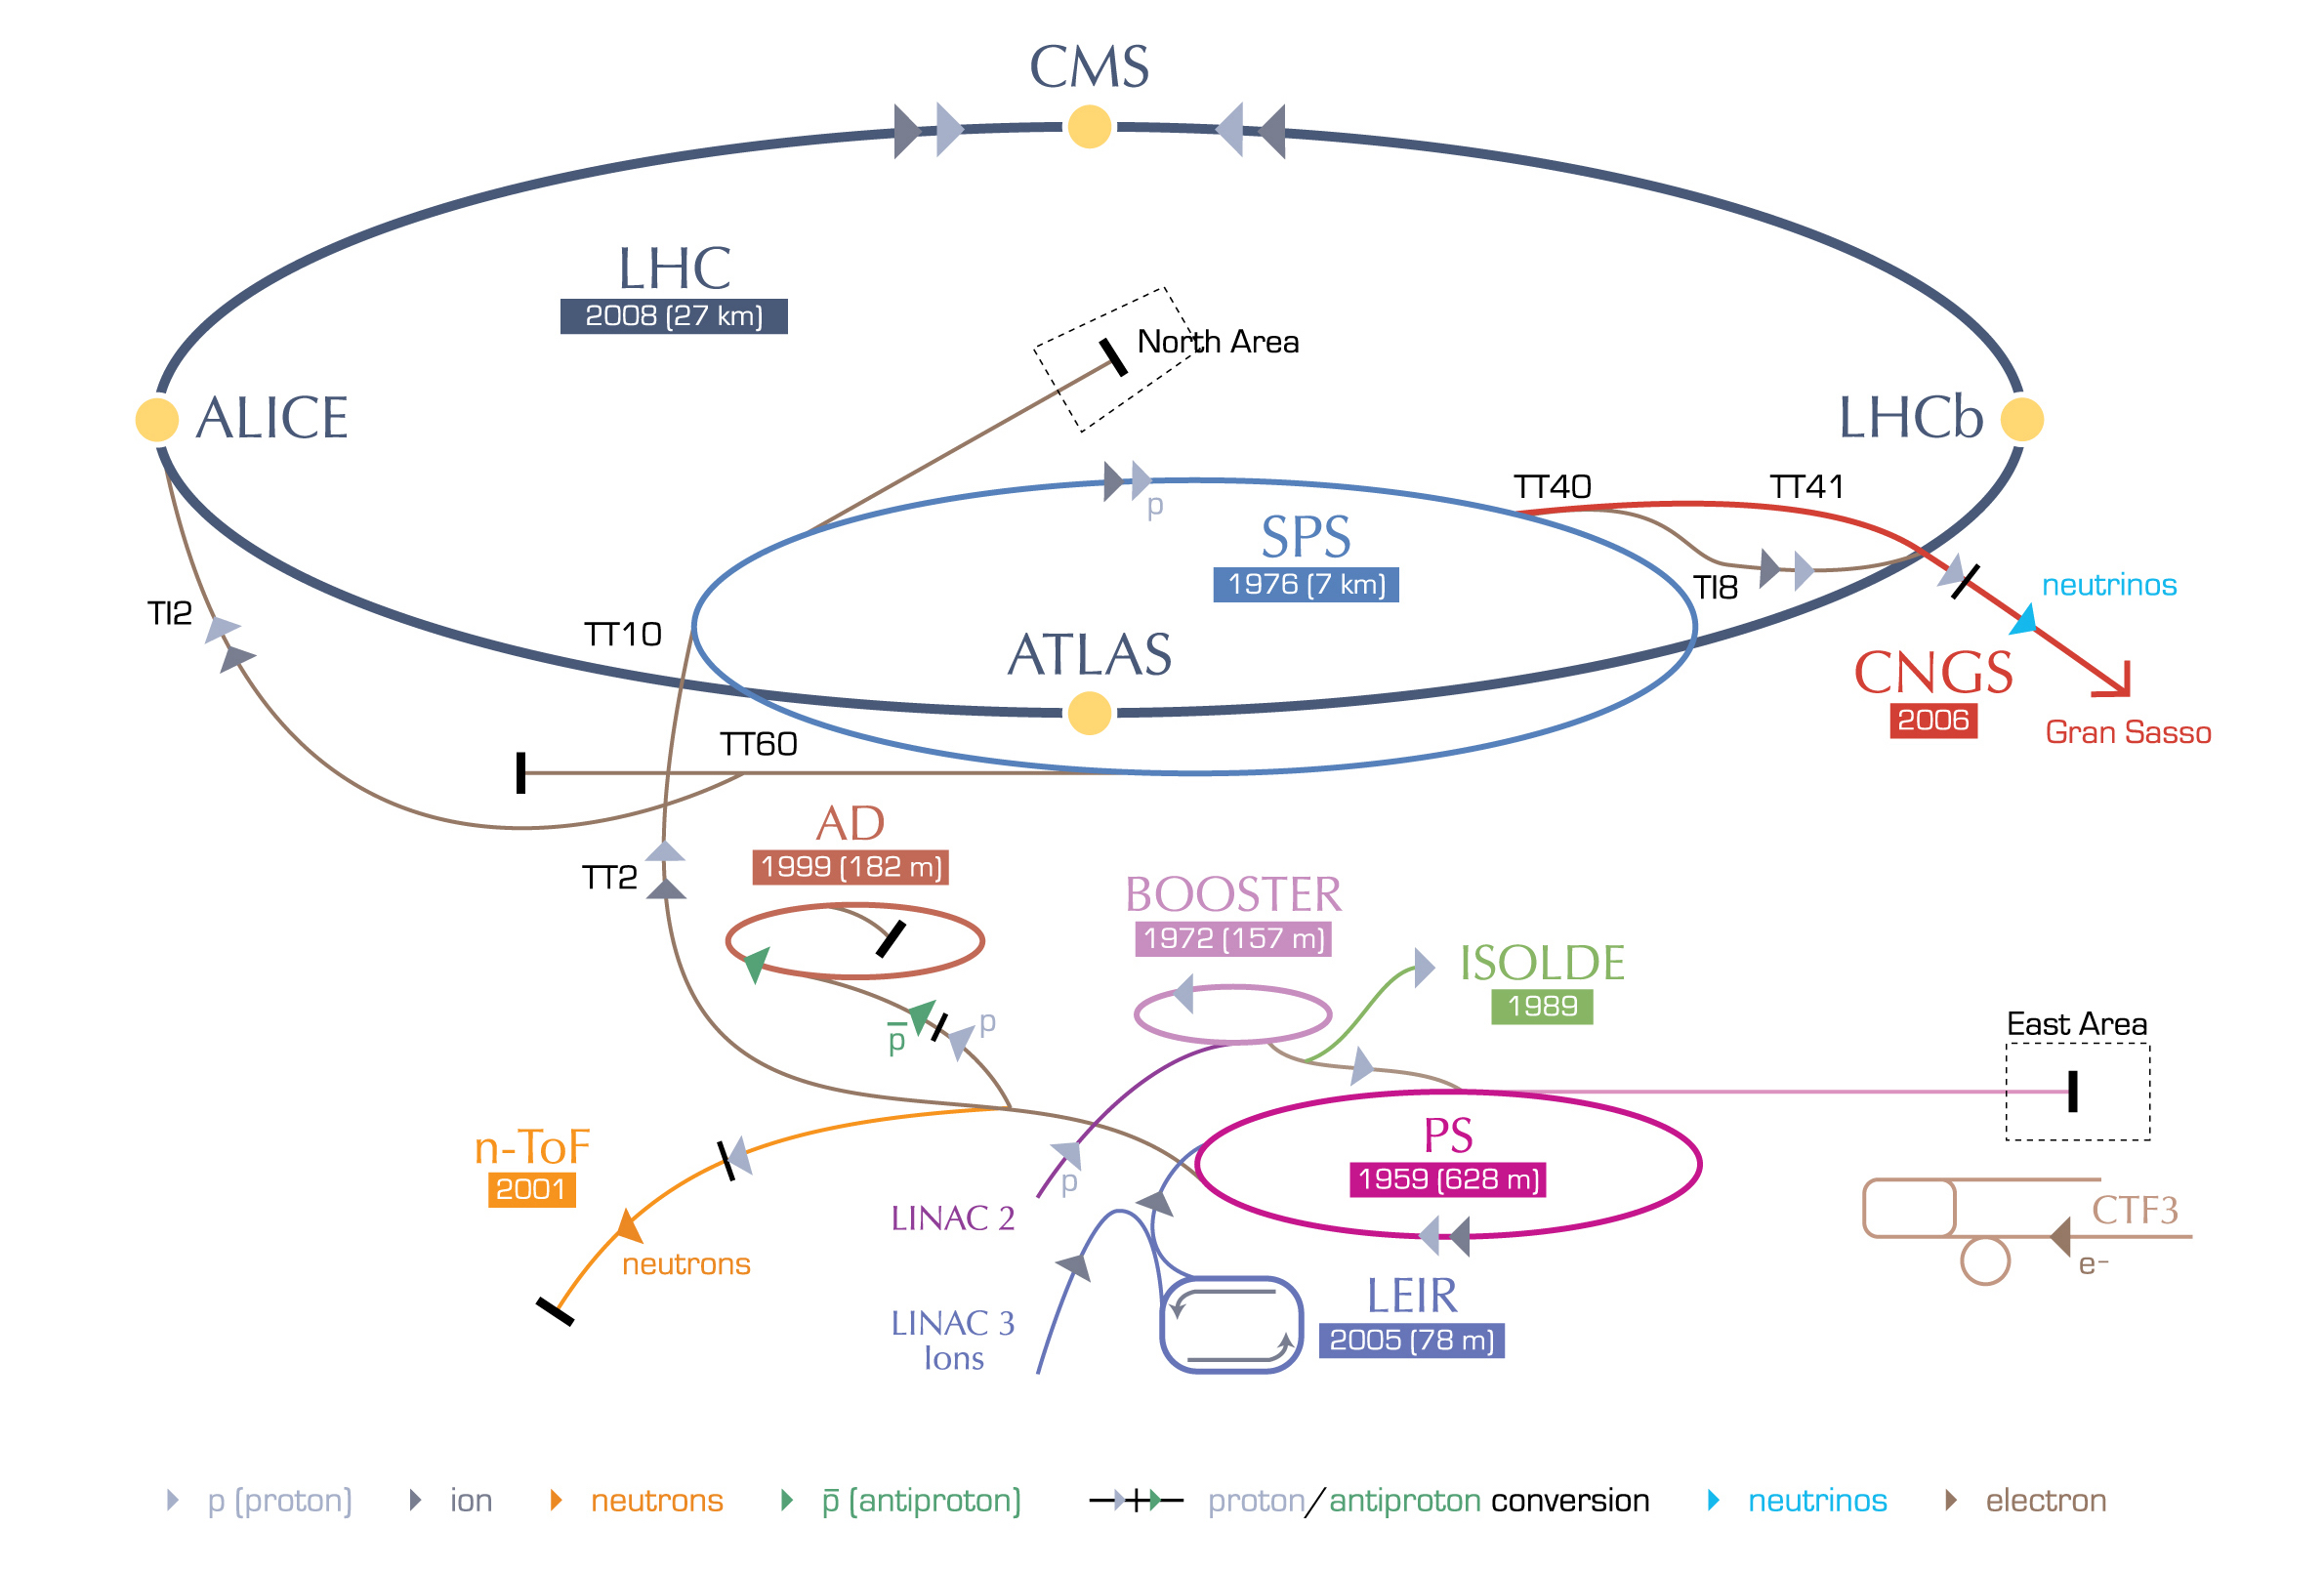
\includegraphics{figures/experiment/accelerator-complex.jpg}
    \newImageResize{figures/experiment/accelerator-complex.jpg}
    \caption{Illustration of the accelerator complex at CERN, including the Linac2, BOOSTER, PS, and SPS that serve as pre-accelerators before the protons are injected into the LHC. Adapted from \ccite{Christiane:1260465}.}
    \label{fig:accelerator-complex}
\end{figure}







\section{The ATLAS Experiment}
The ATLAS experiment is operated by a community of about 3000 scientific authors from 181 institutions and 41 countries~\cite{AtlasCollab}, making it one of the largest scientific collaborations in the world.
This section first provides an overview of the detection principles used to measure the various products of the $pp$ collision events and gives detailed information on the detector setup thereafter.

\subsection{Detection principles}
\label{subsec:measurement-principles}
Different types of particles, such as electrons, muons, or hadrons, originate from the $pp$ collisions and are measured in the ATLAS detector using two main methods: by detecting their trajectories, a method known as \emph{tracking}, and by measuring their energy via total absorption, a principle known as \emph{calorimetry}.

\subsubsection{Tracking}
%To reconstruct the trajectories of charged particles in the ATLAS detector, 
Tracks from charged particles can be reconstructed by measuring discrete space points and recognizing patterns.
The mostly non-destructive space point measurements are provided by detecting the signals (or \emph{hits}) left by traversing charged particles in finely segmented detector layers with known position. Different techniques are used in the ATLAS detector for this purpose:
\paragraph{Silicon semiconductor sensors} detect electron-hole pairs that are created in a p-n junction when a charged particle traverses the material. They can be segmented very finely and thus deliver precise spatial measurements.
\paragraph{Gas filled detectors} measure the current induced after a charged particle ionises a gas via a wire connected at high voltage. The detectors consist of tubes or chambers with different arrangements of electrodes. Their main advantage is a low material cost which makes them useful for covering large areas. \\
% \paragraph{Transition radiation detectors} are based on gaseous ionisation detectors and additionally measure the transition radiation from charged particles that traverse through material with different dielectric constants. The amount of transition radiation is sensitive to the Lorentz factor, which in combination with a momentum measurement provides the ability to measure the mass of a charged particle. This is useful input for particle identification. \\
\newline
To enable momentum measurements of charged particles, the tracking devices are immersed in magnetic fields that force the particles on a curved path. Their momenta can be determined from the radius of curvature of their reconstructed tracks. The resolution of the momentum measurement deteriorates linearly as the particle momentum increases.
%The following types of tracking devices are used in the ATLAS detector:
%The tracking devices are immersed in magnetic fields that force the charged particles on a curved path, allowing their momenta to be measured through the radius of their reconstructed tracks. 
% to bend the charged particles' trajectories. 
% This allows to measure the momentum of charged particles through the radius of their reconstructed track.

\subsubsection{Calorimetry}
%\emph{Calorimetry} can be defined as the detection principle to measure the energy of physics objects by fully absorbing them in blocks of instrumented material, called calorimeters.

Calorimeters measure the energy of particles by fully absorbing them and transferring their energy to electrical signals.
The ATLAS calorimeter is a so-called \emph{sampling calorimeter} where each of these tasks is handled by a dedicated material.
Layers of high-density \emph{passive material} are predominantly responsible for stopping the particles and are alternated with layers of \emph{active material} that focus on measuring the signals induced by the particles.
The total signal measured is proportional to the energy of the incident particle.

% comment from Mike (should be incorporated now!)
% This description is not strictly correct. It implies that the passive material stops the particles, which is true only as a whole. To be precise, there is also energy loss in the active material but of course much less.
% It is better to say that the absorber initiates showers, which are detected in the active layers. I see that you do this below.
% We can talk about how to re-word this if you want but I would rather you do it.


% Layers of \emph{passive material} stop the particles by initiating a process of repeated interactions with the detector material. They are alternated with layers of \emph{active material} that measure the signals deposited by the particles participating in the shower. 
% The ATLAS detector uses so-called \emph{sampling calorimeters} that comprise alternating layers of \emph{active material}, to actively measure the signals of the showering particles, and highly-dense \emph{passive material}, to initiate the showering and stop the particles.
\paragraph{Calorimeter showers}\mbox{}\\
As an incident particle interacts with the passive layers, a cascade of secondary particles forms.
Each secondary particle carries a fraction of the original energy and itself interacts with the calorimeter. This results in the formation of a \emph{calorimeter shower} that consists of particles with gradually decreasing energy as the shower evolves.
A distinction is made between \emph{electromagnetic showers} and \emph{hadronic showers}.

% The incident particles interact with the absorbers through several mechanisms which results in cascades of secondary particles known as \emph{showers}. 
Electromagnetic showers are initiated by electrons, positrons, and photons and are dominated by interactions through \emph{bremsstrahlung} (photon emission) and electron-positron \emph{pair-production}.
%The repeated process of emitting photons (bremsstrahlung) and producing electron-positron pairs (pair-production) forms a cascade of particles with gradually decreasing energy in the detector.
A material can be characterized by its radiation length, $X_0$, which denotes the length over which an electron or positron loses on average all but  $1/e$ of its energy via bremssstrahlung. Since the probability for interacting via bremsstrahlung is proportional to $1 / m^2$, where $m$ is the mass of the particle, muons deposit only a small fraction of their energy in the calorimeters and thus cannot be stopped.\footnote{While muons deposit only a small fraction of their energy in the calorimeters, it is important to consider these energy losses. This becomes more important as the energy of the muon increases, because the amount of energy that is lost due to bremsstrahlung increases with the energy of the muon. See also \cref{sec:muon-reconstruction}.}

Hadronic showers are more complex due to the rich nature of hadronic interactions. An incident hadron initiates showers by inelastic hadronic interactions with nuclei. In the process, several new particles are created, most of which are mesons.
The penetration depth of hadrons in a given material is characterized by their \emph{interaction length}, $\lambda$, which describes the length that a hadron travels on average without interacting.
More details on the characteristics of hadronic showers and their implications for calorimeter energy measurements are left to \cref{chap:calibration}.

\paragraph{Signal detection}\mbox{}\\
% The calorimeter showering as well as the active signal detection is described below.
% Incoming particles interact with the passive material, which initiates a process known as \emph{calorimeter showering}. The active material layers detect the signals of particles inside the showers. When the incoming particle is fully absorbed, the total collected signal is proportional to the initial energy of the particle. 
% \paragraph{Calorimeter showering} occurs when incident particles interact with the passive material through different mechanisms which results in cascades of secondary particles.
The active layers in the ATLAS calorimeter measure the signals from the particles participating in the showers. They consist of either \emph{liquid argon} (LAr) or plastic scintillating tiles.

The LAr-based systems are embedded in cryostats and measure the current induced by ionising particles. Readout electrodes are placed in the liquid and collect the charge within a timeframe of about \SI{450}{\nano\second}. The resulting signal is shown in \cref{fig:LAr-signal-pulse}. The pulse in the detector is first shaped to have a long negative tail in order to reduce the sensitivity to signals caused by $pp$ collisions from neighbouring bunches. The signal is then readout by sampling it four times at \SI{40}{\mega\hertz}. The pulse height is proportional to the energy of the traversing particle and energy calibrations are derived using data from dedicated runs~\cite{Abreu:1303004}.
% so that it can be converted to an energy measurement using calibrations derived from dedicated runs.~\cite{Abreu:1303004}

%In the LAr-based systems, that are embedded in cryostats, the incident charged particles ionise the liquid inducing a current that is measured at electrodes.
In the plastic scintillators, the energy of ionising particles is absorbed by the excitation of atoms and re-emitted in the form of light by the de-excitation of atoms. Also, photons produce light by exciting atoms after undergoing electron-positron pair production, Compton scattering, or photoelectric effect, depending on the energy of the photon.\footnote{Pair production dominates at higher energies larger than several \MeV, Compton scattering in the \MeV-range, and the photoelectric effect at lower energies below 1\,\MeV. The exact energy regime depends on the material.}.
The light is routed with wavelength shifting fibers to two photomultiplier tubes where it is converted to an electric pulse via the photoelectric effect. The pulse can be interpreted as an energy measurement with calibrations derived using data from dedicated runs~\cite{PERF-2007-01}.

\FloatBarrier
\begin{figure}[t]
    \newImageResizeHalf{figures/experiment/LAr-pulse-shape-red-dots.png}
    \caption{Signal pulse measured in the LAr detectors with and without pulse shaping. The large (red) dots indicate the positions at which the signal is ideally read out. Adapted from \ccite{Abreu:1303004}.}
    \label{fig:LAr-signal-pulse}
\end{figure}


\subsection{Overview of the ATLAS detector}
% An illustration of the detector is shown in \cref{fig:ATLASlayout}.
The ATLAS detector, illustrated in \cref{fig:ATLASlayout}, is \SI{44}{\meter} long, \SI{25}{\meter} high, and has a forward-backward symmetric geometry covering almost $4\pi$ in solid angle.
Several layers are arranged in a cylindrical structure around the beam axis.
%The different layers serve different functions and complement each other to form a detector system that is able to measure a wide range of physics processes.
The \emph{inner detector} (ID) is the innermost layer and serves as a tracking device surrounded by a large \emph{solenoid magnet}.
A large \emph{calorimeter system} is placed outside the solenoid and stops almost all electromagnetic and hadronically interacting particles.
The outermost part forms the \emph{muon spectrometer} (MS) which is designed to reconstruct muon tracks using large \emph{muon chambers} with \emph{toroid magnets} placed in between.
% to enable muon momentum measurements.

After introducing the ATLAS coordinate system below, the design and functionality of the different components is described in the remainder of this section.
While most of these sections are kept very brief, more details are provided on the calorimeter system, as it is the crucial component for the calibration measurement presented in the subsequent \cref{chap:calibration}.
More information about the ATLAS detector can be found in \ccite{PERF-2007-01}, which this section heavily relies on.

%Some of the detector components are also used to trigger on interesting physics events which is discussed thereafter.
%After describing the ATLAS coordinate system, a description of the tracking devices, the ID and the MS, followed by details on the calorimeter system.
%A combination of these subsystems is used to trigger on interesting physics events which is discussed thereafter.
%This section concludes with a description of the ATLAS simulation infrastructure. 

\begin{sidewaysfigure}
    \newImageResizeCustom{0.8}{figures/experiment/ATLASdetector.jpg}
    \caption[Schematic of the ATLAS detector showing the various subsystems.]{Schematic of the ATLAS detector showing the various subsystems.
        The innermost layers are used for tracking and consist of the silicon \emph{pixel detector}, the silicon \emph{semiconductor tracker}, and the \emph{transition radiation tracker}.
        They are surrounded by a large \emph{solenoid magnet}.
        The calorimeter system is placed outside the solenoid and includes the \emph{LAr electromagnetic calorimeters}, the hadronic \emph{tile calorimeters}, the \emph{LAr hadronic end-caps}, and the \emph{LAr forward calorimeters}.
        The outermost part forms the muon spectrometer which is designed to reconstruct muon tracks, using large \emph{muon chambers}, and is placed in between \emph{toroid magnets}. Taken from \ccite{PERF-2007-01}.}
    \label{fig:ATLASlayout}
\end{sidewaysfigure}

\subsection{The ATLAS coordinate system}
The ATLAS experiment uses a right-handed cartesian coordinate system to describe the hard-scattering processes. The origin is set at the nominal interaction point, which is at the geometrical centre of the ATLAS detector. The $z$-axis is along the beam direction, the $y$-axis points upwards, and the $x$-axis points to the centre of the LHC. The azimuthal angle $\phi$ is measured against the $x$-axis in the $x$-$y$ plane and the polar angle $\theta$ is the angle taken from the beam axis.
Final-state particles of $pp$ collision events are often Lorentz-boosted along the $z$-axis.
This is why the transverse component of the energy, $\ETvec = \ET \hat{n}$, or momentum, $\pTvec = \pT \hat{n}$, are often considered. They are determined by the projection of the total energy or momentum onto the $x$-$y$ plane.
The position of a particle in the $z$-$y$ plane is typically described with the \emph{pseudorapidity} $\eta$, defined as\footnote{For massive objects the \emph{rapidity} $y = \frac{1}{2} \text{ln} \left( \frac{E + p_Z }{E-p_z} \right)$ is used, where $E$ is the energy and $p_z$ the momentum in $z$-direction. The rapidity is approximated by the pseudorapidity for $m \ll E$, which is typically the case in for physics objects in high energy physics.}
\begin{equation}
    \eta = - \text{ln} \left( \tan \left( \frac{\theta}{2} \right) \right).
\end{equation}
This allows for an angular distance measurement $\Delta R$ between particles,
\begin{equation}
    \label{eq:delta-r}
    \Delta R = \sqrt{ \left( \Delta \eta \right) ^2 + \left( \Delta \phi \right) ^2 },
\end{equation}
that is invariant under Lorentz transformations along the $z$-axis.

% Comment Bernd
% Did you want to mention here are boosts along z are very common in pp colisons (which motivates this choice of coordinates)

\subsection{The inner detector}
\label{subsec:inner-detector}
%Charged-particle tracks stemming from the hard scatter can be reconstructed by recognizing patterns in the hits detected in the ID. 
The ID provides information about the charged-particle positions as close as \SI{27.5}{\milli\meter} to the interaction point.
Tracks reconstructed from ID hits are used for momentum measurements, impact parameter determination, as well as primary and secondary vertexing.
%Hits are detected by layers of different silicon-based semiconductor detectors as well as gaseous ionisation tubes, see \cref{subsec:measurement-principles}. 
A schematic view of the ID is shown in \cref{fig:ATLASinnerdetector}.
In the central (barrel) region the tracking detectors are arranged in cylinders around the beam axis, while in the end-cap regions, the different layers are placed on disks perpendicular to the beam axis.
The ID covers a range \absetaST{2.5} and is immersed in a \SI{2}{\tesla} magnetic field that is provided by a \SI{5.8}{\m} long solenoid magnet.
The first tracking layer in the barrel is the insertable $b$-layer (IBL)~\cite{ATLAS-TDR-19,PIX-2018-001}, that was installed before \RunTwo and is especially important for the reconstruction of the interaction vertices.
Three layers of silicon \emph{pixels} in the barrel and each end-cap typically provide four space points for each charged particle.
Four layers (nine layers) of silicon-microstrip \emph{semiconductor trackers} (SCT) in the barrel (each end-cap) are composed of double layers of strips arranged at an angle of \SI{40}{\milli\radian} relative to each other. Four double layers are crossed by each track to provide additional four space points.
The fine granularity of the pixel and microstrip sensors provide high-precision measurements with resolutions in $R$-$\phi \times z$ ($R$-$\phi \times R$) of $10 \times 115\,\mu\text{m}$ and $17 \times 580\,\mu\text{m}$ for the pixel and microstrip barrels (end-caps), respectively.
The \emph{transition radiation tracker} TRT consists of a large number of straw tubes filled with xenon-based gas that provide on average 36 additional hits. The TRT covers a range \absetaST{2.0} and provides information in only the $R$-$\phi$ plane with a resolution of \SI{130}{\micro\meter}.
Apart from the position measurement, the TRT also generates and detects the amount of transition radiation, that is produced by high-energy charged particles when crossing two media of different dielectric constants. For this purpose, the TRT is interleaved with fibres and foils that provide the transition-radiation photons, which helps to differentiate electrons from charged pions.

% FROM MIKE:
% It would be good to add a couple of sentences to explain what TR is and how it is generated, e.g. there is a radiator in the detector.
% But don’t go overboard and describe the guts of TR generation. It is sufficient to say that it is a relativistic effect that is important only for electrons in ATLAS.

\FloatBarrier
\begin{sidewaysfigure}[t]
    %\resizebox{\textwidth}{!}{
    \subfloat[central region]{
        %\newImageScale{figures/experiment/ATLASinnerdetector.pdf}{.105}
        \newImageScale{figures/experiment/ATLASinnerdetector.pdf}{.155}
    }
    \subfloat[end-cap region]{
        \newImageScale{figures/experiment/ATLASinnerdetectorendcap.png}{.135}
        %\newImageScale{figures/experiment/ATLASinnerdetectorendcap.png}{.095}
    }
    %   }
    \caption{Schematic of the ATLAS inner detector in (a) the central region and (b) the end-cap region, showing the different systems: the IBL (not shown for the end-cap region), the pixel detector, the SCT, and the TRT. Taken from Refs.~\cite{ATL-PHYS-PUB-2015-009} and~\cite{PERF-2007-01}, respectively.}
    \label{fig:ATLASinnerdetector}
\end{sidewaysfigure}




% • They are versatile detectors. Although originally conceived as devices for energy measurement, they can be used to determine the shower position and direction, to identify
% different particles (for instance to distinguish electrons and photons from pions and
% muons on the basis of their different interactions with the detector), and to measure the
% arrival time of the particle. Calorimeters are also commonly used for trigger purposes,
% since they can provide fast signals that are easy to process and to interpret

\subsection{The calorimeter system}
\label{subsec:calorimeter}
The primary task of the ATLAS sampling calorimeter is to measure the energy of particles, but it is also sensitive to the position and direction of incident particles. The latter is enabled by the segmentation of the calorimeter into different cells in the $\eta-\phi$ plane and into several layers in the longitudinal direction.
This also allows quantifying other characteristics of the showers, which is used for particle identification (see \cref{chap:objects}).
The calorimeter signals provide fast information, which makes them also suitable for trigger purposes, which is described further below.

A schematic view of the calorimeter system is shown in \cref{fig:ATLAScalorimeters}.
It can be divided into a \emph{LAr electromagnetic calorimeter} (ECAL), that targets the measurement of electromagnetic showers, and a hadronic calorimeter, that measures and contains hadronic activity. The hadronic calorimeter is further subdivided into the scintillator \emph{tile calorimeter}, the \emph{LAr hadronic end-caps} (HEC), and the \emph{LAr forward calorimeters} (Fcal).
The entire system covers a large angle of \absetaST{4.9} with different materials used in different \abseta regions due to changing conditions.
Depending on the \abseta region, the ECAL and hadronic calorimeter provide a stopping power of $22-38\,X_0$ and $7-10\,\lambda$, respectively.
This limits the level of punch-through to the muon system almost entirely, except for the irreducible level of muons and neutrinos. % remain irreducible. the irreducible level of muons and neutrinos.
A summary of the most important material characteristics of the different segments is shown in \cref{tab:calorimeter-characteristics}.
Details on the detector coverage and granularity are given in \cref{tab:ATLAScalorimeter-parameters}.

\FloatBarrier
\begin{table}[h!]
    \centering
    \begin{tabular}{l | l l l}
        \toprule
                                                 & Active material               & Passive material         & Coverage                \\
        \midrule
        %LAr electromagnetic calorimeter barrel &  liquid argon     & lead             & $\approx 24 X_0$    & \absetaST{1.475}         \\
        %LAr electromagnetic calorimeter end-cap &  liquid argon     & lead             & $\approx 22 X_0$    & \absetaBT{1.375}{3.2}    \\
        LAr electromagnetic                      & \multirow{2}{*}{Liquid argon} & \multirow{2}{*}{Lead}    & \multirow{2}{*}{\absetaST{3.2}} \\
        calorimeter                              &                               &                          &                                 \\
        \midrule
        Tile calorimeter                         & Plastic scintillators                 & Steel                    & \absetaST{1.7}                  \\
        \midrule
        LAr hadronic end-caps                    & Liquid argon                  & Copper                   & \absetaBT{1.5}{3.2}             \\
        \midrule
        \multirow{2}{*}{LAr forward calorimeter} & \multirow{2}{*}{Liquid argon} & Copper (1st layer)       & \multirow{2}{*}{\absetaBT{3.1}{4.9}}             \\
                                                 &                               & Tungsten (2nd/3rd layer) &             \\
        \bottomrule
    \end{tabular}
    \caption[Characteristics of the different calorimeter systems of the ATLAS detector.]{
        Characteristics of the different calorimeter systems of the ATLAS detector, including the active and passive material used, and their \abseta coverage. Taken from \ccite{PERF-2007-01}.}
    \label{tab:calorimeter-characteristics}
\end{table}
%%%%%%%%%%%%%%%%%%%%%%%%%%%%%%%%%%%%%%%%%%%%%%%%%%%%%%%%%%%%%%%%
% Version with stopping power


% \begin{table}
%     \centering
%     \begin{tabular}{l | l l l l}
%         \toprule
%                                                  & Active material               & Passive material      & Stopping power                          & \abseta coverage                     \\
%         \midrule
%         %LAr electromagnetic calorimeter barrel &  liquid argon     & lead             & $\approx 24 X_0$    & \absetaST{1.475}         \\
%         %LAr electromagnetic calorimeter end-cap &  liquid argon     & lead             & $\approx 22 X_0$    & \absetaBT{1.375}{3.2}    \\
%         LAr electromagnetic                      & \multirow{2}{*}{Liquid argon} & \multirow{2}{*}{lead} & \multirow{2}{*}{$\approx 22-38\,X_0$}   & \multirow{2}{*}{\absetaST{3.2}}      \\
%         calorimeter                              &                               &                       &                                         &                                      \\
%         \midrule
%         Tile calorimeter                         & Scintillators                 & Steel                 & $\approx 7-10\,\lambda$               & \absetaST{1.7}                       \\
%         \midrule
%         LAr hadronic end-caps                    & Liquid argon                  & Copper                & $\approx TBD\,\lambda$                 & \absetaBT{1.5}{3.2}                  \\
%         \midrule
%         \multirow{4}{*}{LAr forward calorimeter} & \multirow{4}{*}{Liquid argon} & Copper                & $\approx 28\,X_0$ /                     & \multirow{2}{*}{\absetaBT{3.1}{4.9}} \\
%                                                  &                               & (1st layer)           & $\approx 3\,\lambda$                  &                                      \\
%                                                  &                               & Tungsten              & \multirow{2}{*}{$\approx 7\,\lambda$} & \multirow{2}{*}{\absetaBT{3.1}{4.9}} \\
%                                                  &                               & (2nd/3rd layer)       &                                         &                                      \\
%         \bottomrule
%     \end{tabular}
%     \caption{
%         Characteristics of the different calorimeter systems, including the active and passive material that is used, the approximate stopping power in terms of either the radiation length ($X_0$) or interaction length ($\lambda_0$) depending on whether the system targets electromagnetic or hadronic showers, and the \abseta coverage.
%         The stopping power is given as a range as it strongly depends on the $\eta$ region. \cite{PERF-2007-01}}
%     \label{tab:calorimeter-characteristics}
% \end{table}

\subsubsection{LAr electromagnetic calorimeters}
The ECAL is arranged in an accordion-shaped structure to ensure full coverage in $\phi$.
It is subdivided into a barrel part covering \absetaST{1.475} and an end-cap on each side in the range \absetaBT{1.375}{3.2}.

The barrel consists of two identical segments along the $z$-axis with a small gap of \SI{4}{\milli\meter} in between at $z=0$. A schematic of one of the barrel modules is shown in \cref{fig:ATLASmodules-a}. Each module is segmented in three layers in depth with varying granularity.
The first layer is finely segmented in $\Delta \eta$ which provides essential inputs for photon and neutral pion identification. The second layer is finer in $\Delta \phi$ and larger in depth and measures the bulk of the electromagnetic showers. The third and coarsest layer in $\Delta \eta$ is designed to measure the broad tail of the electromagnetic showers.
%Together, the three segments provide a stopping power of 24 radiation lengths ($X_0$) 
The high granularity provides valuable space point measurements in addition to the data from the ID, reduces the sensitivity to \pileup, and allows handling of large collision rates.

% Comment MIKE: It is also a matter of rate capability and reducing sensitivity to pileup.

% Previously more precise but too many numbers
% The first layer provides high resolution in $\Delta \eta$ with cell sizes of only $0.025 / 8 \times 0.1$ in $\Delta \eta \times \Delta \phi$. This provides essential inputs for photon and pion identification. The second layer measures the bulk of the electromagnetic showers and is finer in $\Delta \phi$ with cell sizes of $0.025 \times 0.025$ in $\Delta \eta \times \Delta \phi$. The third and coarsest layer in $\Delta \eta$ is designed to measuring the broad tail of the electromagnetic showers.
%Together, the three segments provide a stopping power of 24 radiation lengths ($X_0$) 
%The high granularity provides valuable space point measurements in addition to the data from the ID.

% - Accordion-shaped sampling detector (to provide full coverage in eta) with lead as absorber and LAr as active material.
% - EM cal with barrel in eta < 1.475 and end-cap 1.375 < eta < 3.2. 
% - Barrel has small gap of (4 mm) at z = 0. 
% - barrel module Shown in Figure. Three layers with varying granularity very useful for additional position measurement.
In the transition region between the barrel and end-caps (\absetaBT{1.37}{1.52}), also known as the ``crack'', there is a lot of material amounting to several $X_0$ in front of the calorimeter, which renders photon and electron identification difficult.

The end-caps consist of wheels placed on each side of the barrel.
They are composed of three layers in depth for the range \absetaST{2.5} and two layers for \absetaBT{2.5}{3.2} with varying thickness of the lead absorber. Details on the readout granularity is shown in \cref{tab:ATLAScalorimeter-parameters}.

To account for the energy that particles lose upstream of the ECAL, when traversing the ID and solenoid magnet, a presampler consisting of a thin LAr layer is placed in front of the ECAL in the range \absetaST{1.8}.

% - end-caps are two wheels. 
% - Transition region between barrel and endcap known as "crack", rendering photon and electron identification difficult. 
% - "lead thickness optimized has three segments in eta < 2.5 and two section in depth for eta > 2.5."
% - Presampler: "to correct for energy lost by electrons and photons upstream of the calorimeter for eta < 1.8 presampler detector consisting of a thin LAr layer of 1.1cm (0.5cm) thickness in barrel (end-cap)."
% "correct energy losses due to material in inner detector."
% "account for energy lost by electrons and photons traversing the ID and solenoid"
% - high-resolution measurement of electrons, photons.

\subsubsection{Hadronic tile calorimeter}
The hadronic tile calorimeter consists of a \emph{tile barrel}, that is placed directly outside the ECAL and extends to \absetaST{1.0}, and a \emph{tile extended barrel} on each side, covering \absetaBT{0.7}{1.7}.
Their granularity is much coarser than that of the ECAL (see \cref{tab:ATLAScalorimeter-parameters}).
%They provide a stopping power of around 7-10 interaction lengths depending on the $\eta$ region.
%The tile barrel surrounds the barrel of the ECAL and uses steel as absorber with scintillator tiles in between. 

A single module of the tile barrel is shown in \cref{fig:ATLASmodules-b}, depicting the alternating layers of plastic scintillator and steel. The scintillating light induced by traversing particles in the scintillators is collected at photomultipliers mounted on the tile edges via wavelength-shifting fibers. This allows for almost perfect $\phi$ coverage.

\subsubsection{LAr hadronic end-caps}
The HEC provides a coverage of \absetaBT{1.5}{3.2} and is segmented in two layers in depth. It consists of one end-cap wheel on each side of the detector. See Table 3.3 for details of the design.

\subsubsection{LAr forward calorimeter}
At very large angles (\absetaBT{3.1}{4.9}) the calorimeter needs to be especially resistant against radiation. The FCal consists of three thick absorber layers. The first layer targets measurements of electromagnetic showers, the second two provide necessary stopping power for hadrons.

% - LAr forward cals for both EM and HAD up to eta = 4.9. 
% - need to be especially resistant against radiation
% - 10 interaction lengths with three high-density modules per end-cap.
% - first is copper for EM measurements, the other two made out of tungsten for hadrons.



\begin{figure}
    \newImageScale{figures/experiment/ATLAScalorimeters.jpg}{.3}
    \caption[Schematic of the ATLAS calorimeters showing the different subcomponents.]{Schematic of the ATLAS calorimeters showing the different subcomponents. Details on are provided in the text. Taken from \ccite{PERF-2007-01}.}
    \label{fig:ATLAScalorimeters}
\end{figure}

\begin{figure}
    \subfloat[]{
        \newImageResizeCustom{0.53}{figures/experiment/barrel_module.png}
        \label{fig:ATLASmodules-a}
    }
    \subfloat[]{
        \newImageResizeCustom{0.43}{figures/experiment/tile_module_readout.png}
        \label{fig:ATLASmodules-b}
    }
    \caption{(a) Schematic of a single module of the electromagnetic calorimeter illustrating the different layers and their changing granularity as well as an indication of the accordion-like shape. (b) Schematic of a single module of the hadronic tile calorimeter showing the optical readout channels. Taken from \ccite{PERF-2007-01}.}
    \label{fig:ATLASmodules}
\end{figure}

\begin{table}
    \newImageResize{figures/experiment/calorimeter-specs.png}
    \caption{Main parameters of the calorimeter system. Taken from \ccite{PERF-2007-01}.}
    \label{tab:ATLAScalorimeter-parameters}
\end{table}



\subsection{The Muon Spectrometer}
Muons are minimum-ionising particles and escape the calorimeter system.
%Therefore, a large MS forms the outermost part of the ATLAS detector. 
The main purpose of the large MS therefore is to measure muon-track hits for muon reconstruction but also to provide information of a potential muon candidate to the trigger system.
\Cref{fig:ATLASmuonspectrometer} shows the MS including the large superconducting toroid magnets that are located in between several gaseous muon chambers.
The 8 barrel toroid magnets and 16 end-cap magnets cover the range \absetaST{1.4} and \absetaBT{1.6}{2.7}, respectively. They provide magnetic bending power of \numrange{0.5}{1}\,T to measure the muons' momenta. Precision-tracking chambers operate with an argon-based mixture and are arranged in three layers in both the barrel and end-cap regions. They cover a range \absetaST{2.7} and mostly consist of \emph{Monitored drift tubes}, that provide six to eight $\eta$ measurements. Only the innermost layer at \absetaBT{2}{2.7} is made out of multiwire proportional chambers called \emph{Cathode strip chambers} that are more resistant to radiation damage. They provide four space points in the $\eta$-$\phi$ plane. The detector chambers with fast readouts consist of \emph{Resistive-plate chambers} (RPCs) in the central-region within \absetaST{1.05} and \emph{Thin-gap chambers} (TGCs) in the end-cap regions at \absetaBT{1.05}{2.4}.
Their main purpose is to provide information to the Level 1 trigger system (discussed below in \cref{sec:trigger-system}), but also to provide information complementary to the precision trackers to allow for a three-dimensional track reconstruction of the muon candidates.

% They provide information about traversing muons to the L1 trigger system that is discussed below within \numrange{15}{25}\,ns.
%The RPCs are gaseous parallel electrode-plates without a wire and 

\FloatBarrier
\begin{figure}[t]
    \newImageScale{figures/experiment/ATLASmuondetector.png}{.15}
    \caption{Schematic of the ATLAS muon spectrometer. Taken from \ccite{PERF-2007-01}.}
    \label{fig:ATLASmuonspectrometer}
\end{figure}



\subsection{Trigger System}
\label{sec:trigger-system}
It is technically not feasible to store the detector response for each collision event that occurs every \SI{25}{\nano\second}.
A dedicated trigger system therefore makes fast decisions and selects only events for readout which exhibit interesting features.
The selections are based on the available data from various detector subsystems.
% It uses different detector systems and reduces the rate of events selected for readout to \SI{1}{\kilo\hertz}. 
% and selects them for readout. 
%The nominal rate of collision events of produce much more data to be stored than is technically feasible. 
The \RunTwo trigger system consists of a two-stage approach:
The hardware-based \emph{Level-1} (L1) trigger reduces the rate of collision events from \SI{40}{\mega\hertz} to \SI{100}{\kilo\hertz} and provides inputs to the software-based \emph{High-level trigger} (HLT), implemented in a large dedicated computer farm, which makes further selections to reduce the rate to around \SI{1000}{\hertz}.

The L1 trigger uses information from both, the full MS and the entire calorimeter system but with reduced granularity.
The muon trigger chambers (RPCs and TGCs) detect muons with high transverse momenta, while the showering information from the calorimeters is used to search for electrons, photons, jets, hadronically decaying \tauleptons, as well large missing or total transverse energy.\footnote{The definition and reconstruction procedure of these physics objects are described in \cref{chap:objects}.}
By adjusting the identification criteria and thresholds used for the different objects, the trigger rates for different event signatures can be controlled.
Events with certain signatures such as high-\pT jets or large missing transverse energy often occur more frequently than desired for readout. In these cases the related triggers can be \emph{prescaled} by a certain factor to only select one out of many events of that type\footnote{The decision which event is read out is randomized to avoid possible biases}. This enables a controlled data collection as running conditions change.\footnote{All events with at least one identified electron, muon or large missing transverse momentum are \emph{unprescaled}.}
In addition to reducing the event rate, the L1 trigger defines \emph{Regions-of-interest} (ROIs) in the $\eta$-$\phi$ plane to locate the interesting features.
The HLT analyzes the detector signals in the ROIs performing ``offline-like'' full event reconstruction using all detector subsystems with their full granularity. The ROIs typically make up around \SI{2}{\percent} of the total event data.
The events selected by the HLT are subsequently stored to disk.
More information on the ATLAS trigger system can be found in \ccite{ATLAS-TDR-16,ATLAS-TDR-12,PERF-2007-01}.

% Goal:
% - Nominal rate of collisions much higher than the maximum that can be stored
% - Most types of events not interesting
% - Trigger / select the interesting events for read out
% Physics / Technology Exploited:
% - Different detector systems with fast readout at play
% Technical Details:
% - L1 trigger defines ROIs in eta - phi space where it detects interesting features
% - High-level trigger (HLT) analyzes ROIs and makes further selections
% - So-called pre-scaling available
% From ATLAS paper: "The L1 trigger searches for signatures from high-pT muons, electrons/photons, jets, and tau-leptons decaying into hadrons. It also selects events with large missing transverse energy (Emiss)
% and large total transverse energy. The L1 trigger uses reduced-granularity information from a
% subset of detectors: the Resistive Plate Chambers (RPC) and Thin-Gap Chambers (TGC) for high-
% pT muons, and all the calorimeter sub-systems for electromagnetic clusters, jets, tau-leptons, Emiss, T
% and large total transverse energy."
% From Arnold: "
% The L1 trigger decision is based on coarse-granularity measurements provided by a limited set of the detector subsystems, i.e. the EM and hadronic calorimeters as well as the muon trigger chambers, RPC and TGC."
% - HLT further processes inputs from L1 using all detector subsystem with their full granularity. Only the ROIs identified by the L1 trigger are processed.
% - In the HLT only the ROIs identified by the L1 are further analyzed, but using all detector subsystems with their full granularity.


\subsection{Detector simulation}
Simulations of the ATLAS detector are required in order to generate full Monte Carlo events that can be compared to actual experimental data.
The simulations need to consider the response of each individual detector system, the effect of material placed throughout the detector, detector imperfections, as well as data and trigger conditions.
The ATLAS detector simulation is based on \textsc{Geant4}~\cite{Agostinelli:2002hh}.
% From Deep Learning and its applications in physics
%In the language of statistics and machine learning, the full simulation chain would be considered a generative model for the data as they can be used to generate synthetic data of the same complexity and format as the actual collision data.
%Due to the complexity of the experiment a \emph{full simulation} is a very computing-intensive process. The ATLAS simulation infrastructure also allows for \emph{fast simulations} using simplified descriptions of the detector systems. This provides the opportunity for lower processing times with the drawback of decreased accuracies.
The simulations produce data of the same complexity and format as the actual experimental data, so that the same software can be used for further processing of the events.
More information on the ATLAS simulation infrastructure can be found in \ccite{ATLAS-TDR-17,SOFT-2010-01}.
%- full simulation of particle interaction with matter throughout detector 



\section{Data Acquisition during 2015-2018}
\label{sec:run-2-data-taking}

\Minote{}{I should mention the detectors that measure the luminosity}

The operation of the LHC during \RunTwo between April 2015 and December 2018 was a great success and even exceeded the goals set in terms of luminosity production. At a centre-of-mass energy of $\sqrt{s} = 13\,\TeV$, the peak instantaneous luminosity was more than twice as high as its design value reaching up to $\instLumi = \SI{2.1e34}{\per\cm\per\s}$ in 2018.
\Cref{fig:run-2-data-taking-a} shows the integrated luminosity delivered by the LHC (156\ifb), recorded by the ATLAS detector (147\ifb), and certified as being of ``good'' data quality (139\ifb).
The recorded luminosity reflects the small inefficiency of the data acquisition infrastructure as well as the fact that the ATLAS detector is fully activated for readout only after a short ramp-up period in the tracking detectors that is started once the LHC produces stable beam collisions.
The recorded data are further filtered before being considered for physics analyses.
An event is considered ``Good for Physics'' if all reconstructed objects satisfy certain data-quality requirements and if it was recorded at times when all relevant detector components were fully operational.
The integrated luminosity that is analyzed by physics analyses makes up 89\% of the total delivered luminosity.
More information on the data quality monitoring framework can be found in \ccite{DAPR-2018-01}.

Due to changing running conditions, the distribution of the mean number of interactions per bunch crossing varies between the years.
The distributions are shown in \cref{fig:run-2-data-taking-b}.
Noticeable is the double-peak structure of the data recorded in 2017.
An alternative beam production scheme had to be used because of an issue in the beam vacuum for some periods in this year\footnote{In 2017, during the replacement of a dipole magnet seven liters of air entered the beam vacuum. The water vapor froze at the interconnection of cell 16L2 which lead to unstable beams that were dumped early~\cite{Jimenez:2646067,Salvant:2646056}. More information can be found in \ccite{Steerenberg:2696126}.}. This resulted in particularly high pile-up conditions of up to 60-70 interactions per bunch crossing and thus the mentioned double-peak structure.
% In 2017, the LHC performance was hampered by the so-called 16L2 issue: frozen air in an interconnection between magnets in the arc connecting Point 1 (ATLAS) with Point 2 (ALICE)In 2017, the LHC performance was hampered by the so-called 16L2 issue: frozen air in an interconnection between magnets in the arc connecting Point 1 (ATLAS) with Point 2 (ALICE)
More details on the LHC running conditions during \RunTwo can be found in \ccite{Steerenberg:2696126}.

\TDinote{}{Should I make the lumi plots larger? Mike's preference}
\TDinote{}{Make sure pile-up is defined beforehand}

\begin{figure}[t]
    \subfloat[]{
        \newImageScale{figures/reconstruction/run2-lumi.pdf}{.36}
        \label{fig:run-2-data-taking-a}
    }
    \subfloat[]{
        \newImageScale{figures/reconstruction/run2-pileup.pdf}{.36}
        \label{fig:run-2-data-taking-b}
    }
    \caption{(a) Collected luminosity and (b) Mean number of interactions per crossing for $pp$ collisions during \RunTwo of the LHC. More information is provided in the text. Taken from \ccite{PublicLumiResults}.}
    \label{fig:run-2-data-taking}
\end{figure}

% Caption from ATLAS (https://twiki.cern.ch/twiki/bin/view/AtlasPublic/LuminosityPublicResultsRun2#Multiple_Year_Collision_Plots)
% Number of Interactions per Crossing
% Shown is the luminosity-weighted distribution of the mean number of interactions per crossing for the 2018 pp collision data at 13 TeV centre-of-mass energy. All data recorded by ATLAS during stable beams is shown, and the integrated luminosity and the mean mu value are given in the figure. The mean number of interactions per crossing corresponds to the mean of the poisson distribution of the number of interactions per crossing calculated for each bunch. It is calculated from the instantaneous per bunch luminosity as μ=Lbunch x σinel / fr where Lbunch is the per bunch instantaneous luminosity, σinel is the inelastic cross section which we take to be 80 mb for 13 TeV collisions, and fr is the LHC revolution frequency. The luminosity shown represents the preliminary 13 TeV luminosity calibration for 2018, released in February 2019, that is based on van-der-Meer beam-separation scans. Data collected by ATLAS for the entire 2018 run through the end of October are shown.

% Total Integrated Luminosity and Data Quality in 2015-2018
% Cumulative luminosity versus time delivered to ATLAS (green), recorded by ATLAS (yellow), and certified to be good quality data (blue) during stable beams for pp collisions at 13 TeV centre-of-mass energy in 2015-2018. The complete pp data sample in 2018 is shown. The delivered luminosity accounts for the luminosity delivered from the start of stable beams until the LHC requests ATLAS to put the detector in a safe standby mode to allow a beam dump or beam studies. The recorded luminosity reflects the DAQ inefficiency, as well as the inefficiency of the so‐ called "warm start": when the stable beam flag is raised, the tracking detectors undergo a ramp of the high-voltage and, for the pixel system, turning on the preamplifiers. The data quality assessment shown corresponds to the All Good efficiency shown in the 2015-2018 Full Dataset DQ tables here. The All Good Data Quality criteria require all reconstructed physics objects to be of good data quality.


% %-------------------------------------------------------------------------------

\chapter{Physics Object Reconstruction and Identification}
\label{chap:objects}

Due to the complex phenomenology of $pp$ collisions and the high luminosities at the LHC the ATLAS detector is exposed to enormous particle multiplicities. It is therefore challenging to correctly interpret the detector signals recorded for a given bunch crossing and accurately reconstruct the different \emph{physics objects} that are produced.
Reconstructed physics objects represent both elementary particles such as electrons, muons, or photons, and composite particles such as \emph{jets} or quantities derived using the entire event information like the \emph{missing transverse energy}.
The ATLAS experiment uses a variety of sophisticated reconstruction and identification algorithms\footnote{Reconstruction algorithms are implemented within the extensive ATLAS software suite~\cite{ATL-SOFT-PUB-2021-001}.}, that are under constant development, to reconstruct these physics objects, and describes them with four-vectors.
% that are constantly being improved, 
%like jets or quantities derived using the entire event information like missing transverse energy.
This chapter provides details on the algorithms used to reconstruct and identify the physics objects relevant for the work presented in this thesis.

\Minote{}{Maybe I want to explicitely mention the chapters: First two chapters outline basic reconstructions that are used in object reconstructions, jets, electrons and photons, muons, missing et}

% - section tracks and calorimeter clustering describes the procedure that reconstructs the ingredients for further object reconstruction. Then the physics objects are explained, starting with jets, electrons and photons, as well as muons and missing tranverse energy.
%The event reconstruction can be broadly divided into two stages: a reconstruction step which includes energy calibrations, and an identification process, where the reconstructed objects are identified with physics objects as well as an origin, which also includes the resolution of ambiguities present in the reconstruction step.

% - Carsten: "algorithms under constant development as they greatly influence the efficiency and performance of the reconstruction process".
% - Arnold: "This raw data is then processed in several steps by various, sophisticated reconstruction and identification algorithms implemented in the ATHENA framework [170] in order to finally identify the measured signals with physics objects, such as electrons or jets, defined by relatively few parameters."
% - Valente: "These four-vectors are generally known as the physics objects of the collision as they represent the quarks, leptons and gauge bosons resulting from the p-p collisions of the LHC."
% - Ruthmann: "The event and object reconstruction chain is defined and implemented in the Athena software framework [75]."
% - Dickinson talks about final state and the associated particles -> maybe a good idea? Good segway to explain that tau lepton reconstruction is not explained in the thesis


\section{Inner Detector Tracks and Vertex Reconstruction}
The charged-particle hits measured in the ID are used to build tracks that are input to further reconstruction algorithms.
The track reconstruction uses a sequence of pattern recognition algorithms that are described in much more detail in \ccite{Cornelissen:1020106,Cornelissen_2008}. The sequences primarily consist of a so-called \emph{inside-out} algorithm and an \emph{outside-in} algorithm.

%They complement each other in the tasks to find tracks associated to the hard-scatter interaction (inside-out algorithm), and tracks stemming from secondary decay vertices in the ID as well as tracks from photon conversions (outside-in algorithm).
The inside-out algorithm is seeded by three hits in the silicon detectors. An initial track collection is formed based on a window search and a combinatorial Kalman filter~\cite{fruhwirth_application_1987}. Two more steps follow: First, the ambiguities in the initial track collection are resolved, and then the tracks are extended to hits in the TRT without manipulating the original tracks from the silicon detector measurements. Tracks reconstructed with the inside-out algorithm can be considered as the trajectories of charged particles originating from the interaction region.

The outside-in algorithm starts with a global pattern recognition from all TRT hits. The identified segments are then traced back into the silicon detectors, excluding any hits already used in the inside-out stage. The outside-in algorithm is designed to reconstruct tracks stemming from secondary vertices in the ID, for example, from heavy-flavour hadron decays or from photons converting into an electron-positron pair via pair-production.

% The track reconstruction efficiency, defined as the fraction of charged particles with $\pT > 400\,\MeV$ and \absetaST{2.5} that are matched to a reconstructed track, has only a small dependence on the number of pile-up interactions and is well above \SI{70}{\percent} for a range \absetaST{2} and pile-up conditions of $\mu = 41$~\cite{ATLAS-CONF-2012-042}. \Mnote{}{Not sure if I should mention this here. Should I then also mention the PV reco efficiency? Don't know yet. Probably not? Cause of this written in Sommers thesis: "The efficiencies shown in Fig. 3.1b is obtained in simulated events that also contain collisions with low momentum transfer. The efficiency to reconstruct the vertices of the interactions studied in this thesis is close to 100 percent". Also track reconstruction probs not useful as it does not reflect the high pT muons}

The reconstructed tracks are also used to determine the positions of the collision vertices, known as \emph{primary vertices} (PV). To this end, an \emph{iterative vertex finding} approach \cite{PERF-2015-01} starts with selecting tracks that both satisfy certain quality criteria and are compatible with the interaction region. A vertex seed is chosen based on the density of the selected tracks and is input to an \emph{adaptive vertex fitting} algorithm~\cite{0954-3899-34-12-N01}.
This algorithm iteratively (re-)fits tracks and seeds new vertex candidates if a track is incompatible with the currently assigned vertex.
%A new vertex needs to have at least two associated tracks. 
This process continues until either all tracks are associated to a vertex or no further vertex candidates can be built.
All vertices with at least two associated tracks are kept as valid PV candidates.
%This algorithm iteratively (re-)fits tracks including the constraint that they originate from that vertex, and seeds a new vertex candidate if they are incompatible. This is repeated until either all track are associated to a vertex or no further vertex candidates can be built, which requires at least two associated tracks.
Once the PVs are found, the \emph{hard-scatter vertex} is chosen to be the one with the largest sum of squared track transverse momentum. The other PVs are classified as \emph{pile-up vertices}.

To classify whether the tracks originate come from the hard-scatter vertex or from pile-up vertices, two variables are used: the transverse and longitudinal impact parameters, labelled as $d_0$ and $z_0$, respectively. They are defined as the distance of closest approach of the track to the hard-scatter vertex along the transverse plane ($d_0$) and $z$-axis ($z_0$).

% - "reference comes from a reference given in the latest electron reco publication (CERN-EP-2019-145) where a reference is given to the tracking: \ccite{PERF-2015-08}."
% - long reference: \ccite{Cornelissen:1020106}
% - shorter summary in journal: \ccite{Cornelissen_2008}
% - in thesis I used this reference \ccite{ATLAS-CONF-2012-042} that describes the algorithms briefly

% \Minote{}{Think about whether I should mention the reconstruction efficiency. <- current tendency is NO! -> NO!}


\section{Calorimeter Clustering}
\label{sec:calo-clustering}
Each cell of the calorimeter system is read out and interpreted as a massless four-vector. In the first reconstruction step of calorimeter deposits, the cells are grouped together to form so-called \emph{topological clusters} or \emph{topo-clusters}. Topo-clusters are used as input to further reconstruction algorithms to form jets, electrons, or missing transverse energy, as described in later sections.

The main goal of the so-called \emph{topo-clustering algorithm} is to enhance the signal-to-noise ratio, as the calorimeter cells are subject to significant noise contributions. The total noise can be written as
\begin{equation}
    \sigma_{\text{noise}} = \sqrt{ \left( \electronicnoise  \right)^2  + \left( \pileupnoise  \right)^2 },
\end{equation}
where \electronicnoise is the electronic noise and \pileupnoise is the noise from pile-up that varies for different data taking conditions. \Cref{fig:calo-noise} shows the noise as a function of \abseta. While the electronic noise is comparatively constant across \abseta, the pile-up noise increases as \abseta increases. This is a result of the fact that the cell granularity becomes broader for higher values of \abseta (see \cref{subsec:calorimeter}).
% From https://atlas.web.cern.ch/Atlas/GROUPS/PHYSICS/PAPERS/PERF-2014-07/
% Probs get it from here cause other one is 50ns bunch crossing...
% ATL-LARG-PUB-2008-002 -> Should find out what pile-up is expected with design lumi. Design maximum pile-up is 20!

Topo-clusters are formed based on the cell-energy significance, $z_{\text{cell}}$, defined as the level of signal, $E_{\text{cell}}$, above the total noise,
\begin{equation}
    z_{\text{cell}} = \frac{E_{\text{cell}}}{\sigma_{\text{noise}}}.
\end{equation}
The topo-clustering algorithm consists of three steps, each defined by a threshold value~\cite{PERF-2014-07}:
\begin{enumerate}
    \item \textbf{Finding seeds:} A calorimeter cell is taken as a seed if $|z_{\text{cell}}| > S$.
    \item \textbf{Adding neighbours:} All neighbouring cells that have not been used as seed and satisfy $|z_{\text{cell}}|~>~N$ are added to the seed cell.
    \item \textbf{Finalize: } All neighbouring cells with $|z_{\text{cell}}| > P$ are added.
\end{enumerate}
To provide a considerable noise suppression, the standard values used for the ATLAS calorimeters in \RunTwo are $S = 4$, $N = 2$, $P = 0$, such that the algorithm is sometimes referred to as the ``420 topo-clustering'' algorithm. The exact noise thresholds, that is the values assumed for $\sigma_{\text{noise}}$, that are used for each calorimeter system and $\abseta$ region varies and also depend on the data taking conditions, in particular how many pile-up interactions occur. 

The initial set of clusters identified with the algorithm explained above may have large topo-clusters resulting from the merging of energy depositions due to multiple particles very close to each other in the calorimeter.
Therefore, another processing step, known as \emph{cluster splitting}, is performed to split topo-clusters with two or more local maxima. The details of this procedure are described in \ccite{ATL-LARG-PUB-2008-002}.

After the splitting, the topo-clusters represent three-dimensional energy depositions with energies that correspond to the sum of the energies of the included cells.
%- PLOT: add plots of topo-cluster formation as in Valente's thesis? YES!
The cells are calibrated at the electromagnetic scale (\emph{EM scale}) which means that the energy of electromagnetic interacting particles is correctly taken into account\footnote{The calibration of calorimeter cells is derived in dedicated test-beam measurements described for example in \ccite{Abat_2010}.}. The calorimeter does not fully account for the energy deposited by hadrons, which has important consequences for energy calibrations, which is discussed in more detail in \cref{chap:calibration}.

\begin{figure}
    \subfloat[electronic noise]
    {    \newImageResizeHalf{figures/reconstruction/cells-electronic-noise.png}
    }    \subfloat[total noise]
    {    \newImageResizeHalf{figures/reconstruction/cells-total-noise.png}
    }
    \caption{Noise in calorimeter cells from (a) electronic noise at $\mu=0$ and (b) total noise including pile-up noise at instantaneous luminosities of $\mathcal{L} = \SI{e34}{\per\cm\per\s}$ corresponding to peak pile-up conditions of around $\mu\approx20$. The noise is shown per calorimeter layer: the presampler (PS), the three electromagnetic calorimeter layers (EM1-EM3), the layers of the hadronic tiles (Tile1-Tile3) and end-caps (HEC1-HEC4), and the forward calorimeter layers (FCal1-FCal3). Taken from \ccite{ATL-LARG-PUB-2008-002}.}
    \label{fig:calo-noise}
\end{figure}


\section{Jets}
\emph{Jets} are the experimental manifestation of quarks and gluons.
They consist of collimated sprays of particles in the detector and are abundant at the LHC.
%, originating from the hadronisation of quarks and gluons, 
Almost all physics analyses need to consider jets. Jets can be defined at various stages during their evolution in the detector, as illustrated in \Cref{fig:jet-evolution}. First, the quarks and gluons produced in the collision events undergo a process of parton showering (see \cref{sec:anatomy}) and produce a \emph{parton jet}. The partons then hadronise to form a spray of stable particles referred to as \emph{particle jet}. Finally, the hadrons interact with the detector and initiate particle showers that are eventually measured in the calorimeter. At this stage, the object is called \emph{calorimeter jet} or simply \emph{jet}.
The main challenge of jet physics is to define and calibrate the experimentally measured jet in a way that allows for meaningful comparisons between experiment and theory. 
% describes the original particle jet as accurately as possible.
% Only this will allow meaningful comparisons between experiment and theory.

This section describes the most important aspects of jet reconstruction in the ATLAS experiment.
% A useful characteristic of a jet is its origin, in particular, whether the jet is more likely to stem from the hard-scatter vertex or a pile-up vertex. The strategy to identify so-called \emph{pile-up jets} is discussed further below.
% The information about which hadron a jet originates from, specifically whether a $b$-hadron was involved, is another important metric to characterize and classify different experimental signatures. A description of this process known as \emph{flavour tagging} concludes this section.
The description of how the energy of the reconstructed jets are calibrated is left to \cref{chap:calibration}.

\subsection{Jet definition}
% The main challenge of jet physics is to define the experimentally measured jet in a way that describes the original parton as accurately as possible. \Qnote{}{original parton or particle jet?}
% Only this will allow meaningful comparisons between experiment and theory.
%As a jet is the closest signature of a quark or gluon that can be measured experimentally, special care needs to be taken in its definition to facilitate meaningful comparisons between experiment and theory.
To compare experimental results with theoretical predictions, jet counting is often involved. The jet definition therefore needs to be insensitive to two theoretical divergences:
\begin{itemize}
    \item \emph{Collinear divergence}: the probability for a given quark to emit a gluon along the same axis, known as \emph{collinear splitting}, diverges.
    \item \emph{Infrared divergence}: the probability for a given quark to emit a soft gluon with energies reaching zero, known as \emph{soft emissions}, diverges.
\end{itemize}
A jet definition is said to be both \emph{infrared} and \emph{collinear safe}, when the set of hard jets that is found in a given event remains unchanged when modifying the amount of collinear splitting or soft emissions.
% In other words: jet definition is independent on the presence of partons radiated collinearly to the quark and on soft radiation
In practice, a jet is defined by two choices: the \emph{jet constituents}, that is the set of energy measurements to consider, and a \emph{jet algorithm}, that is the set of rules according to which the constituents are grouped together.

% - A jet is entirely defined by the choice of constituents and the algorithm to group them together.
% - Different definitions come with different strategies for calibrations, etc.  and are also constantly improved. 

\FloatBarrier
\begin{figure}
    \newImageResizeCustom{0.7}{figures/reconstruction/jet-evolution-2.png}
    \caption{Sketch of the evolution of a jet in the detector, highlighting the three distinct stages: parton jet, particle jet, and calorimeter jet. Taken from \ccite{jetEvoReference}.}
    \label{fig:jet-evolution}
\end{figure}
\Minote{}{Replace jet evolution figure.}

\subsubsection{Jet algorithm}
\label{subsubsec:jet-algorithm}
The jet algorithm widely adopted in ATLAS is the so-called \emph{anti-$k_T$} algorithm~\cite{Cacciari:2008gp}, that is both infrared and collinear safe.
In a multi-stage procedure the first step is to take a set of input objects and for all their combinations compute two distinct distance metrics.
The first type of metric is defined as the distance between two objects, labelled as $i$ and $j$,
\begin{equation}
    d_{ij} = \text{min}\left(\frac{1}{p_{T_i}^2},\frac{1}{p_{T_j}^2}\right) \frac{\Delta R_{ij}^2}{R^2},
    \label{eq:dij}
\end{equation}
where $\Delta R$ is defined as shown in \cref{eq:delta-r}; the second type is given by the distance between object $i$ and the beam,
\begin{equation}
    d_{iB} = \frac{1}{p_{T_i}^2}.
\end{equation}
% The \antikt algorithm uses a parameter value of $p = -1$.
The algorithm then assesses the minimum of all the computed values and proceeds as follows:
\begin{itemize}
    \item If the smallest distance is of type $d_{ij}$, the objects $i$ and $j$ are combined, and the algorithm begins again with the list of distances including the one for the newly combined object.
    \item If the smallest distance is of type $d_{iB}$, the object $i$ is considered a jet and is removed from the list of objects. The algorithm then proceeds with finding the new minimum.
\end{itemize}
The procedure is repeated until no objects are left and only jets remain.
The parameter $R$ in \cref{eq:dij} controls the radius and entirely defines the algorithm.
Unless otherwise noted, the jets used in the work presented in this thesis use a radius parameter of $R = 0.4$.
% Typically a minimum pT requirement is used.
%In the \HWW analysis presented in \cref{chap:hww}, a radius  is used. 
%The jet calibration measurements presented in \cref{chap:calibration} consider both, jets with $R = 0.4$ and so-called $R$-scan jets with $R = 0.2$ or $R = 0.6$.


\subsubsection{Jet constituents and definitions of jet collections}
%Jet definitions vary not only depending on the radius parameter used, but also on which inputs (or constituents) are used for the \emph{anti-$k_T$} algorithm. 
%The inputs are known as \emph{jet constituents}. 
Different inputs can be used for the \emph{anti-$k_T$} algorithm.
Historically, the majority of physics analyses used jets reconstructed with only calorimeter information in the form of topo-clusters.
Before the topo-clusters are used in the jet algorithm, they undergo a process known as \emph{origin correction}, in which the positions of the topo-clusters are recomputed to take into account the position of the identified hard-scatter vertex rather than the detector origin.
Jets formed with topo-clusters at the EM scale are referred to as \emph{EMTopo} jets.
%- Mention event-by-event origin correction (in JET section!)
% From JER paper
% Only positive-energy topo-clusters are used as inputs to the jet reconstruction. A jet produced in the hard-scatter process is expected to originate from the primary vertex, defined as the reconstructed vertex with at least two associated tracks and the largest sum of squared track momentum.
% Therefore, an event-by-event correction to account for the position of the primary vertex in each event – referred to as an origin correction – is applied to every topo-cluster, based on its depth within the calorimeter and pseudorapidity. This method is to be contrasted with earlier approaches [7] that applied this correction only to the jet four-momentum rather than to its constituents.
During \RunTwo, the ATLAS collaboration introduced a more sophisticated definition of jets, that uses information from both, the calorimeter and the ID, to exploit the superior measurements of the ID at low transverse momenta.
These jets are known as \emph{particle flow jets} (PFlow jets) and consist of two types of constituents: \emph{charged particle flow objects} (CPFOs) and \emph{neutral particle flow objects} (NPFOs) which are together referred to as \emph{PFlow objects}. The CPFOs consist of high-quality ID tracks that are compatible with the hard-scatter vertex by requiring $|z_0 \sin \theta| < 2$\,mm.
%distance of the closest approach of the track to the hard-scatter vertex along the $z$-axis.
The NPFOs comprise origin-corrected topo-clusters in the calorimeters identified as originating from neutral particles. The algorithm that defines the set of PFlow objects is known as \emph{particle flow algorithm} (PFlow algorithm) and is explained in more detail below. PFlow objects are input to the \antikt algorithm with $R = 0.4$ to form the final set of PFlow jets.
PFlow jets have an improved energy and angular resolution, reconstruction efficiency, and pile-up stability compared to EMTopo jets~\cite{PERF-2015-09}.
\Cref{chap:calibration} discusses the improved jet energy resolution of PFlow jets.

%- Mention truth jets / particle jets here? Constituents: Truth jets are reconstructed using stable final-state particles and exclude muons, neutrinos, and particles from pile-up interactions. Truth jets are selected with the same 𝑝T > 7 GeV and |𝜂| < 4.5 thresholds as EMtopo and PFlow jets, and are geometrically matched to those jets using the angular distance Δ𝑅 with the requirement Δ𝑅 < 0.3. -> probably something unique to calibration measurements (Or is it? If we evaluate uncertainties with truth samples they use truth jets I guess!)

In MC simulated $pp$ collisions, another jet definition is often used by using truth information. With this information, jets at particle-level can be reconstructed. These particle-level jets, also referred to as \emph{truth jets}, are defined with the same jet algorithm as the reconstructed jets, but use all stable final-state particles as inputs except muons, neutrinos, and particles coming from pile-up interactions. They are typically compared to the reconstructed jets by matching them geometrically with a minimum requirement on $\Delta R$.
% Ghost association for track 
% Tracks are matched to jets using ghost association [35], a procedure that treats them as four-vectors of infinitesimal magnitude during the jet reconstruction and assigns them to the jet with which they are clustered.

% - The main goal of particle flow jets is to use the detector as optimally as possible.
% - The tracker provides more precise momentum measurements in the range of 20-40 GeV.



\subsection{The particle flow algorithm}
\label{subsec:pflow-algorithm}
The PFlow algorithm is a multi-stage procedure to identify energy deposits in the calorimeter that are likely to be caused by charged particles. The energy of the topo-clusters that can be clearly associated to a track is not considered in the reconstruction of PFlow jets, but their energy is ``\emph{removed}'' (or ``\emph{subtracted}'') from the calorimeter and instead the \pT of the track is used. A flow chart of the different steps of the algorithm is shown in \cref{fig:pflow-algorithm} and the procedure is outlined below. More information can be found in \ccite{PERF-2015-09} and a description of the changes to the PFlow algorithm introduced for \RunTwo is described in \ccite{JETM-2018-05}.

\subsubsection{Selection of tracks} Tracks considered for the energy subtraction must require stringent criteria: at least nine hits in the silicon detectors and no missing pixel hit when such a hit would be expected~\cite{PERF-2015-09}. They must have \absetaST{2.5} and $\pT < 0.5\,\GeV$ and must not be matched to an electron or muon candidate. A parametrised maximum \pTtrack requirement excludes some tracks with $\pTtrack < 100\,\GeV$ from the algorithm. The parametrisation aims at finding the tracks for which the ID measurements can be assumed inferior to the calorimeter measurements. No track above $\pTtrack = 100\,\GeV$ is considered.

\subsubsection{Matching of tracks to topo-clusters} Topo-clusters with $\Ecluster / \ptrack > 0.1$, where \Ecluster is the energy of the topo-cluster and \ptrack the momentum of the track, are considered for the track-to-cluster matching. The matching is based on a distance metric that takes into account the size of the topo-clusters in $\eta$ and $\phi$. If the topo-cluster that is closest to the track position extrapolated to the second layer of the EM calorimeter falls below a certain distance threshold, it is matched to the track and the track is considered for the energy subtraction.

\subsubsection{Determination of \Eoverpexp} To quantify the amount of energy that is to be subtracted from the calorimeter, the average energy must be known that a track with given \pT deposits in the calorimeter. This quantity, labelled as \Eoverpexp, is determined in a single-pion sample and defines the expected energy that is deposited by a track: $\Edepavg = \ptrack \Eoverpexp$.

\subsubsection{Recovery of split showers} Charged particles may deposit their energy in multiple topo-clusters. In order to identify these cases the difference of the matched topo-cluster energy and the expected value, divided by the expected spread of \Edepavg, labelled as $\sigma \left(E_{\text{dep}}\right)$, is computed:
\begin{equation}
    S(\Ecluster) = \frac{ \Ecluster - \Edepavg}{\sigma \left(E_{\text{dep}}\right)}.
\end{equation}
If $S(\Ecluster)  < -1$, which corresponds to cases in which the deposited energy is significantly lower as expected, additional topo-clusters within a cone of $\Delta R = 0.2$ around the track extrapolated to the second EM calorimeter are considered for the energy subtraction.

\subsubsection{Energy subtraction and remnant removal} If \Edepavg exceeds the energy of the matched clusters, the summed energy of the topo-clusters is removed. Otherwise, the energy of the matched topo-clusters is removed on a cell-by-cell basis. The order in which the cells are removed is based on a measure that quantifies the most likely energy density profile in each layer. Cell energies are subtracted subsequently until the total subtracted energy exceeds \Edepavg. The energies of the remaining cells is then further removed, if they can be assumed to originate from shower fluctuations. This is determined by the requirement that the total subtracted energy is still within $\Edepavg \pm 1.5\,\sigma \left(E_{\text{dep}}\right)$ when the remnants are removed.

\subsubsection{The final set of particle flow objects}
The set of remaining topo-clusters after the last step of the energy subtraction are referred to as NPFOs. 
The tracks considered for the energy subtraction constitute the CPFOs.
% The CPFOs are defined as all the tracks that satisfy $|z_0 \sin \theta| < 2$\,mm, where $z_0$ is the distance of the closest approach of the track to the hard-scatter vertex along the $z$-axis.
% They are input to the \antikt algorithm with $R=0.4$ to form the final set of PFlow jets.

\FloatBarrier
\begin{figure}[t]
    \newImageResize{figures/reconstruction/pflow-algorithm.pdf}
    \caption{Flow chart of the particle flow algorithm. More details are given in the text. Taken from \ccite{PERF-2016-06}.}
    \label{fig:pflow-algorithm}
\end{figure}

\subsection{Pile-up jet identification}
Jets that have an origin other than the hard scatter are classified as pile-up jets.
They are a nuisance to physics analyses as they can spoil the measurements when not being identified correctly.
\Cref{fig:pile-up-jets-illustration} illustrates the two categories of pile-up jets:
\emph{stochastic pile-up jets}, reconstructed from energy deposits randomly clustered in certain regions, and \emph{QCD pile-up jets}, originating from genuine pile-up vertices.\footnote{It should be noted, that this distinction, as well as \cref{fig:pile-up-jets-illustration}, is mainly used for the purpose of a convenient description. The actual experiment is subject to many pile-up interactions such that this boundary is blurred, as every jet also has contributions from pile-up.}
To identify these types of jets a multivariate discriminant called \emph{Jet Vertex Tagger} (JVT)~\cite{ATLAS-CONF-2014-018} is used.
The JVT is based on a combination of two track-based variables that allow to separate hard-scatter jets from pile-up jets. The variables are used to construct a two-dimensional likelihood that corresponds to the relative probability for a given jet to stem from the hard scatter.
To suppress pile-up jets, physics analyses typically require a minimum JVT threshold for jets in the central region \absetaST{2.4} and within a certain \pT range.
%In the work presented in this thesis, this value is set to JVT $> 0.59$. 
The JVT achieves a hard-scatter efficiency that is approximately stable as the number of pile-up interactions increases, identifying about \SI{90}{\percent} hard-scatter jets with a pile-up jet rate of about \SI{1}{\percent}.
JVT calibrations are provided by analysing data from $Z (\rightarrow \mu\mu)$ candidate events.
More information can be found in \ccite{ATLAS-CONF-2014-018}.


\subsection{Jet cleaning}
Jets that have an origin other than the $pp$ collisions may be reconstructed in the detector. They can be caused by coherent calorimeter noise or non-collision backgrounds such as cosmic rays or beam-induced backgrounds. To reject these types of jets a procedure known as \emph{jet cleaning} is applied. To this end, several jet quality criteria are considered that are based on three categories of variables: pulse shape variables of the LAr calorimeter, energy ratio variables considering deposits in different layers of the calorimeter as well as \fEM, and track-based variables.
Applying basic selections on these variables yields a high efficiency exceeding \SI{99}{\percent} for selecting the jets from the $pp$ collisions and rejects a significant portion of jets with different origins. More information can be found in \ccite{ATLAS-CONF-2015-029}.


\FloatBarrier
\begin{figure}[t]
    \newImageResize{figures/reconstruction/pile-up-jets-illustration.pdf}
    \caption{Illustration of an event containing a hard-scatter (HS) jet, a QCD pile-up (PU) jet, and a stochastic pile-up jet. The $\Delta \text{R}_{\text{pT}}$ observable allows to distinguish QCD pile-up jets from stochastic pile-up jets, based on the fraction of total jet energy stemming from charged particles in the jet. The figure is taken from \ccite{PERF-2016-06}, where more information on the observable can be found.}
    \label{fig:pile-up-jets-illustration}
\end{figure}


\subsection{Flavour tagging}
\label{subsec:flavour-tagging}
The process of classifying a jet as originating from a certain quark flavour is known as \emph{flavour tagging}, which is a crucial ingredient for many physics analyses. Especially important for the work presented in this thesis is the identification of jets that originate from $b$-quarks, called $b$-\emph{jets}.

Different jet-related properties can be used for $b$-jet identification.
%, called \emph{$b$-tagging},
%about the underlying physics process that occurred.
%provide information about the likelihood that a given jet originates from a certain quark flavour.
%This in turn is crucial input to classify different hard scatter events.
The $b$-jets contain $b$-hadrons that have a relatively long lifetime of about \SI{1.5}{\pico\second} before they decay. This, in addition to the fact that energetic $b$-jets typically experience a large Lorentz boost, leads to the formation of a secondary decay vertex that is far enough away from the hard-scatter vertex for it to be detectable with the track and vertex information from the ID.
Several low-level \emph{$b$-tagging algorithms} primarily exploit this distinct detector signature\footnote{Also other characteristics of the production and decay of $b$-hadrons are considered, such as the high $b$-hadron mass, the (charged) decay multiplicity, or $b$-quark fragmentation properties.}, to identify (or \emph{tag}) jets as $b$-jets. They also make use of other information such as impact-parameter measurements or reconstructed secondary vertices~\cite{ATL-PHYS-PUB-2017-013}.

The outputs of the low-level taggers are used to construct a final discriminant that provides a likelihood that a given jet is a $b$-jet. The work presented in this thesis uses a deep neural network discriminant, denoted as DL1r, that is trained with inputs from four low-level taggers~\cite{ATL-PHYS-PUB-2017-013}.
By requiring jets to have a minimum DL1r output value, different $b$-jet tagging efficiencies can be obtained. The efficiencies are calibrated with simulated \ttbar events~\cite{FTAG-2018-01}.
Because the algorithms rely on ID information, only jets with \absetaST{2.5} can be considered for $b$-jet identification.



\section{Electrons and Photons}
\label{sec:electron-photon-reconstruction}
Electrons and photons are reconstructed from topo-clusters mostly formed in the EM calorimeter\footnote{In the crack between the EM barrel and end-caps also information from the hadronic tile calorimeter and presampler is used.} and tracks from the ID~\cite{EGAM-2018-01}.
In a simplified picture, an electron can be defined as a topo-cluster that is associated to a track and a photon as a topo-cluster without a matched track.
However, photons can convert to an electron pair in the ID by pair production\footnote{About \SI{20}{\percent} of photons convert at low \abseta in the ID, and up to \SI{65}{\percent} at $\abseta \approx 2.3$~\cite{EGAM-2018-01}.} and electrons may radiate photons via bremsstrahlung, which makes distinguishing the two objects more challenging. Electron and photon reconstruction is therefore based on the formation of so-called \emph{superclusters}, that take into account the effects of both pair production and bremsstrahlung. The multi-stage algorithm to form superclusters is explained in the following.

In the first step, tracks that are loosely matched to topo-clusters are refitted accounting for bremsstrahlung. Refitted tracks as well as photon-conversion vertices\footnote{The algorithm to reconstruct conversion vertices is documented in \ccite{PERF-2017-02}. Minor changes were introduced for \RunTwo, which is described in \ccite{EGAM-2018-01}.} are then matched to topo-clusters.
This is input to the supercluster formation algorithm, which is performed independently for electrons and photons.
Electron (photon) superclusters are seeded by topo-clusters with $\pTGT{1}\,\GeV$ ($\pTGT{1.5}\,\GeV$) that are matched to tracks with at least four hits in the silicon detector (without any track requirement).
The seed topo-clusters are extended by secondary topo-clusters that capture the energy that may be deposited by photons from bremsstrahlung or may appear as part of a split topo-cluster due to converted photons.
The final electron and photon superclusters consist of a seed topo-cluster and associated secondary topo-clusters and are then matched to tracks and conversion vertices, respectively.
Because the supercluster formation is performed independently between electrons and photons, potential ambiguities between the track-matched superclusters occur. A procedure to resolve the ambiguities classifies a given track-matched supercluster as an electron candidate only, a photon candidate only, or as either an electron or photon candidate.
Objects falling in the latter category are explicitly marked ambiguous, which provides the freedom for analyses to tailor the classification criteria based on their specific requirements.
The energy of the final electron and photon candidates is calibrated with \Zee events, which is described in more detail in \ccite{EGAM-2018-01}.

Information about the origin of the reconstructed electrons and photons is crucial for physics analyses.
Electrons stemming from the hard scatter are referred to as \emph{prompt} electrons. They need to be distinguished from other signatures with similar energy deposits such as jets or converted photons, as well as from \emph{non-prompt} electrons produced in heavy-flavour hadron decays.
Similarly, prompt photons from the hard scatter are important to separate from jets or photons produced within jets.
To this end, different quantities are defined and grouped into two sets of criteria: \emph{identification criteria}, that characterize the quality of the reconstructed detector signals produced by electrons and photons themselves, and \emph{isolation requirements}, that describe the activity near the reconstructed objects in order to reject non-prompt electrons and photons or signatures falsely identified as such. A brief overview is given below. More details can be found in \ccite{EGAM-2018-01}.

\subsection{Electron and Photon Identification}
A likelihood discriminant is defined to identify electrons~\cite{EGAM-2018-01}. It is based on several quantities characterizing the shower shape in the EM calorimeter, the track conditions, the amount of energy deposited in the hadronic calorimeters, and the track-cluster compatibility. Different so-called operating \emph{working points} for identification are defined and tuned to achieve a certain efficiency for electron reconstruction. The efficiency for each working point is approximately constant across different detector regions and energies of the electron.
Similar identification criteria and working points are defined for photon identification. They are mostly based on shower shape variables.

\subsection{Electron and Photon Isolation}
Quantities describing the activity near electrons and photons provide important information about the event signature. They are based on track information as well as calorimeter information.
The track isolation variable, \pTcone, quantifies the activity around the electron track or assumed photon direction by summing all transverse momenta within a cone centered around the track axis or photon direction, respectively. The cone can be of fixed size, for example $R=0.2$, labelled as \pTconetwenty, or variable size, labelled as \pTvarcone. In the latter case the radius is given by $\Delta R = \text{min} \left( 10 / (\pT \text{[\GeV])}, \Delta R_{\text{max}}  \right)$, with $R_{\text{max}}$ typically set to $R_{\text{max}} = 0.2$.
The calorimeter isolation, \ETconetwenty, sums the transverse energy of topo-clusters found within a cone of typically $R=0.2$ centered around the electron or photon superclusters.
Different working points are defined and calibrated for typically a combination of track-based and calorimeter-based isolation requirements.
%This provides the freedom to choose isolation criteria based on the individual analyses requirements.

% Single sentence in paper:
% Leptons are required to be isolated from other activity in the event using maximum thresholds on both energy (using close-by clusters in the calorimeter) and 𝑝T (using close-by tracks). 

\section{Muons}
\label{sec:muon-reconstruction}
Muons leave traces in the ID and the MS and deposit only a small fraction of their energy in the calorimeters.
Different strategies exist to reconstruct muons that use different detector subsystems and algorithms~\cite{MUON-2018-03}.
In the work presented in this thesis, muons are reconstructed from a global fit of matching ID tracks and separately reconstructed MS tracks and also taking into account the energy losses in the calorimeters.

Standalone MS tracks are reconstructed starting from straight-line track segments identified in the layers of the precision muon chambers (MDTs and CSCs).
These segments are combined by considering additional information from the hard scatter vertex, the magnetic field, and information from the trigger detectors (RPCs and TGCs). The MS tracks are then matched to ID tracks and an iterative global track fitting procedure finds the final set of muon tracks, by also taking into account energy losses in the calorimeter as well as effects due to possible misalignments of the chambers, and resolving track ambiguities.
% The muon momentum scale and resolution are calibrated using \Jpsimumu and \Zmumu events by exploiting the known mass of the $Z$ boson~\cite{PERF-2015-10}.

\subsection{Muon Reconstruction and Isolation}
To select high-quality muon candidates several identification criteria are defined.
Requirements are primarily based on the number of hits in the ID and MS, the compatibility between the ID and MS tracks, and track fit properties~\cite{MUON-2018-03}.

To select muons from the hard scatter (prompt muons) and reject muons originating from hadron decays or pile-up interactions (non-prompt muons), several variables are defined to quantify how isolated a given muon is.
The isolation requirements are similar to the ones defined for electrons and photons and typically use a combination of track-based isolation and calorimeter-based isolation requirements.
Further criteria are posed on the impact parameters of the muon tracks, to ensure that the muon is compatible with stemming from the hard-scatter vertex.
The reconstruction, identification, and isolation efficiencies are derived using \Jpsimumu and \Zmumu candidate events~\cite{MUON-2018-03}.

%( From master thesis)
% To calibrate the momentum scale of muons, dimuon decays of the Z boson or other known mass resonances are exploited. The identification efficiency and the trigger efficiency of the muon trigger system is measured using almost pure Z → μμ or J/Ψ → μμ samples with a tag-and-probe method [70].

% (Rom Master thesis)
% Different muons are categorized in Loose, Medium and Tight with increasing purity, based on the
% 4.4 Lepton Isolation 29
%  quality of reconstruction and identification criteria. Additionally there is a selection especially suited for High-pT muons [70].
% To calibrate the momentum scale of muons, dimuon decays of the Z boson or other resonances, where the mass is known, are considered. The identification efficiency and the trigger efficiency of the muon trigger system is measured using almost pure Z → μμ or J/Ψ → μμ samples with a tag-and-probe method [70].

% From CONF
% For muons, a quality-based identification method [25] is employed, selecting the “Tight” working point with an efficiency of ∼95% so as to maximise the sample purity. The impact parameter requirements are |𝑧0 sin𝜃| < 0.5 mm and |𝑑0|/𝜎𝑑0 < 5 (3) for electrons (muons)2. Leptons are required to be isolated from other activity in the event using maximum thresholds on both energy (using close-by clusters in the calorimeter) and 𝑝T (using close-by tracks). At least one of the offline reconstructed leptons must be matched to an online object that triggered the recording of the event. In the case where the 𝑒–𝜇 trigger is solely responsible for the recording of the event, each lepton must correspond to one of the trigger objects. This trigger matching scheme also requires the 𝑝T of the lepton to be at least 1 GeV above the trigger level threshold.


\section{Missing Transverse Energy}
\label{sec:met}
The colliding protons do not carry a significant amount of transverse energy prior to the collision events.
The vectorial sum of all transverse energy measured in the detector is therefore expected to be approximately zero for a given event, unless particles are present that are invisible to the detector. The computation of missing transverse energy, labelled as \ETmissvec, thus provides an effective mechanism to indirectly measure neutrinos or other non-interacting particles.
The \ETmissvec observable can be written as
\begin{equation}
    \ETmissvec = - \left( \sum_{\text{obj}} \vec{E}_{\text{T}}^\text{ obj} + \vec{E}_{\text{T}}^\text{ soft-term} \right)
    % = - \sqrt{ \left( E_{\text{x}} \right)^2 + \left( E_{\text{y}} \right)^2 } \hat{e}_{E_{\text{T}}} 
    = \ETmiss \hat{u}_{\ETmiss}
    \label{eq:met}
\end{equation}
and consists of two main contributions: The so-called \emph{hard term}, $\vec{E}_{\text{T}}^\text{ obj}$, that takes into account all fully reconstructed and calibrated physics objects such as electrons, photons, $\tau$-letpons, muons, and jets, and the \emph{soft term}, $\vec{E}_{\text{T}}^\text{ soft-term}$, that sums all energy or momentum measurements that cannot be assigned to any physics object.
Since most physics processes are invariant under $\phi$ translations, the magnitude, \ETmiss, is typically referenced instead of the vector quantity \ETmissvec.
In the work presented in this thesis, the soft term is determined by the sum of \pT of all ID tracks that are associated to the hard-scatter vertex.

An alternative definition of \ETmiss referred to as missing transverse momentum or \pTmiss uses tracks for the hard term, replacing the fully reconstructed objects.
For certain physics analyses, the \pTmiss observable shows slightly better discrimination power against certain event signatures that need to be rejected (see for example \cref{chap:hww}). The standard \ETmiss as defined in \cref{eq:met}, however, has a superior resolution and is thus more widely adopted in ATLAS.
The performance of \ETmiss reconstruction is studied with event samples very pure in events with genuine \ETmiss ($W \rightarrow e\nu$) and without genuine \ETmiss (\Zmumu)~\cite{PERF-2016-07}.

% 2. \emph{calorimeter-based soft-term} (CST): sum of calorimeter clusters not assigned to any physics objects.
% - CST MET is used for building signal-sensitive variables such as mT because its lower resolution.
Since \ETmiss measurements are based on the entire detector, it is a complex quantity to determine precisely. Detector inefficiencies and resolution effects can lead to mismeasurements of the true \ETmiss.
Another observable known as \emph{missing transverse energy significance}, $S$, therefore assesses the probability of the \ETmiss to originate from only these irreducible causes.
% Another quantity is therefore defined that assesses the probability of the \ETmiss to originate from only these aforementioned, irreducible causes.
% The observable is called \emph{missing transverse energy significance}, labelled as $S$, and helps to detect events where non-interacting particles are present.
% A large value of S is an indication that a particle escaped the detector without being detected.
A simple definition of $S$ is given by $\METSigsimple = \ETmiss / H_{\text{T}}$, where $H_{\text{T}}$ is the sum of scalar \pT of all objects in the event.
A more sophisticated approach is given by the so called \emph{Object-based Missing transverse energy significance}, \METSigobject, that takes into account the resolution effects of the measured physics objects.
More details about this quantity can be found in \ccite{ATLAS-CONF-2018-038}.


% From MASTER
% The soft-term is either calculated by using charged-particle tracks originating from the primary vertex using the information of the ID and denoted as \emph{track-based soft-term} (TST), or utilizes the non-assigned calorimeter clusters in the \emph{calorimeter-based soft-term} (CST).

% From Paper:
%  The missing transverse momentum Etmiss (with magnitude E miss ) is defined as the negative vector sum of TT
%  the pT of all the selected leptons and jets, together with reconstructed tracks that are not associated with
%  these objects but are consistent with originating from the primary pp collision [32]. A second definition
%  of missing transverse momentum (in this case denoted pmiss) uses tracks also for the hadronic hard term, T
%  replacing the calorimeter-measured jets with their associated tracks instead. The pmiss observable is used T
%  directly in the selection of events because of its ability to discriminate better against the Z/γ∗ → ττ
%  background, while the Emiss observable is used to build signal-sensitive variables such as mT due to its superior 
% resolution.




% % % ---------------------------------------
\chapter{Measurement of the Jet Energy Resolution}
\label{chap:calibration}
\Minote{}{Refer to theory section, see comment in .tex file}
% As seen in the anatomy section, particle interaction probabilities vary by a huge span. This necessitates a precise knowledge of the detector and resolutions of measurements. Things like Pile-up are a nuisance in this endeavor, also seen in the anatomy section, and needs to be properly accounted for.
The SM of particle physics makes predictions about the dynamics of quarks and gluons, yet these particles cannot be directly measured in the detector. Quarks and gluons hadronize to form hadrons which give rise to particle showers in the detector that are reconstructed as jets.
While \cref{chap:experiment} focused on the experimental setup to measure the signals deposited by hadrons, and \cref{chap:objects} described how the signals are reconstructed to form jets, this chapter gives an overview of the procedures that are used in the ATLAS experiment to calibrate the energy of measured jets. Only calibrated jets allow making meaningful comparisons between experimental measurements and theoretical predictions.
The experimentally measured jet is calibrated to the level of the particle jet. The calibration is experimentally challenging due to the rich environment at hadron colliders as well as the complicated nature of hadronic interactions in the detector. The intricacies of how the detector responds to incoming particle showers is therefore first described in \cref{sec:detector-response}. \Cref{sec:jes-calibration} then describes the multi-stage procedure to calibrate the energy of PFlow jets and EMTopo jets to the scale of the particle jet, which is known as the \emph{jet energy scale}, or \emph{JES}.
It is also crucial to measure the \emph{jet energy resolution}, or \emph{JER}, i.e., the precision with which the energy of a jet can be measured. \Cref{sec:jer} introduces how the JER can be parametrized and \cref{sec:jer-measurement} discusses how the ATLAS collaboration measures the JER in data from \RunTwo for PFlow jets and EMTopo jets, respectively. Particular focus is given on the measurement of the noise term of the JER, which arises due to both multiple pile-up interactions and electronic noise. \Cref{sec:jer-in-analysis} concludes this chapter with a description of how the measured JER is used in physics analyses.
%  and \cref{sec:improvements-jer-measurement} gives an outlook on potential future improvements for the JER measurements.

% is crucial in order to be able to correct the JER in MC such that it matches the one found in data.

% This chapter describes how jet calibration is facilitated at the ATLAS experiment. 
% how experimental jets relate to partons.
%As a jet is the closest signature of a quark or gluon that can be measured experimentally, special care needs to be taken in its definition to facilitate meaningful comparisons between experiment and theory.
%how MC simulations need to be calibrated to match the data.

%- Paper: paper presents the strategy used for the determination of the jet energy scale (JES) and resolution (JER) by the ATLAS experiment and its implementation as it pertains to the analysis of data from Run 2 of the LHC.

%- This publication focuses on calibrating jets reconstructed with the anti-𝑘𝑡 [1] algorithm with radius parameter 𝑅 = 0.4.


\section{Detector Response to Jets}
\label{sec:detector-response}
The response of the calorimeter to traversing particles is defined as the fraction of the particle's original energy that can be measured. The so-called \emph{jet response} is thus the average detector response to the showering particles that form the jet.
As mentioned in \cref{chap:objects}, the calorimeter cells are calibrated at the EM scale which means that electromagnetically interacting particles like photons and electrons are measured with a response of $e = 1$. The energy of hadrons cannot be fully captured and some fraction of the energy does not contribute to the calorimeter signals, resulting in a hadron response of $h < 1$. Various physics effects contribute to this behavior, that is known as \emph{non-compensating}.
%The calorimeter is therefore referred to as being  and 
\begin{itemize}
    \item The showering hadrons can transfer energy to atomic nuclei that may be broken up during the interaction or remain in excited states. This energy is lost in the binding energy or the excited states of the nuclei.
    \item The showering hadrons may decay to non-interacting secondaries that escape the detector, for example in pion decays to a muon and a neutrino.
    \item Neutrons may be produced which mostly undergo elastic scattering and thus escape the detector.
\end{itemize}

The particle showers of a jet consist of both an EM component and a non-EM component. The EM component consists of EM sub-showers created by pions that halt the hadronic decay chain by decaying into pairs of photons. The non-EM component includes all hadronic interactions.
The full jet response can be written as
\begin{equation}
    R(E) = e\fEM(E) + h\left(1 - \fEM(E)\right),
\end{equation}
where \fEM is the fraction of the jet that interacts electromagnetically. This fraction increases as the energy of the jet increases, because the number of possibilities to produce neutral pions increases. The calorimeter response is therefore \emph{non-linear} with increasing jet energy.

In addition to the aforementioned effects, that lead to a calorimeter that is non-compensating, other factors related to the experiment and reconstruction contribute to potential energy mismeasurements:
\begin{itemize}
    \item Non-functional (\emph{dead}) detector material.
    \item Inefficiencies in the topo-clustering algorithm.
    \item Energy deposits that are not taken into account due to the finite radius of the jet algorithm.
\end{itemize}

To determine the jet response in the experiment, the reconstructed jet \pT can be compared to the \pT of a well-calibrated or well-known \emph{reference object}. The reference object may constitute a well-measured physics object or system in data, as explained in \cref{subsec:insitu-calibration}, or a particle-level truth jet, that is accessible in MC simulation.
In the latter case, the truth jets are typically matched geometrically to the reconstructed jets by requiring them to be within a certain radius $\Delta R < R_{\text{matched}}$.
The so-called \emph{truth response} can then be defined as the ratio of the reconstructed jet \pT and the \pT of the matched truth jet,
\begin{equation}
    R_{\text{truth}} =  \frac{\pTreco}{\pTtruth},
\end{equation}
which is a useful quantity for calibrating the jet energy, which is explained in the next section.
%When the energy of the reconstructed jet is calibrated so that $\pTreco = \pTcalib$, the mean jet response is what is considered to be the jet energy scale (JES) and the width of the jet response constitutes the jet energy resolution (JER). The mean and width are determined from a Gaussian fit to the core of the response distribution, as shown in \cref{fig:truth-response}. 


\section{Jet Energy Corrections}
\label{sec:jes-calibration}
The goal of the jet energy correction is to correct for the non-linearity as well as the non-compensating nature of the calorimeter and to bring the average jet response to unity.
To this end, a calibration procedure is performed that consists of several stages. The procedure used to calibrate jets reconstructed with the \antikt algorithm with a radius parameter of $R = 0.4$ is illustrated in \cref{tab:jes-calibration} and is discussed in this section. At each stage, the jet is manipulated at the level of the fully reconstructed object which is represented as a massless four-vector. The energy of a jet can therefore be treated as equivalent to its momentum\footnote{The terms energy and momentum are thus often used interchangeably throughout this thesis}. More details on the calibration procedure can be found in \ccite{JETM-2018-05}.

\begin{table}
    \newImageResize{figures/calibration/jes-calibration.pdf}
    \caption{Summary of the different stages of the jet energy calibration. Each correction is applied to the four momentum of the jet. Taken from \ccite{JETM-2018-05}.}
    \label{tab:jes-calibration}
\end{table}

%The different steps use either MC simulation or data and are also applied to either MC or data, depending on the correction.
\subsection{Pile-up correction}
\label{subsec:pile-up-correction}
The reconstructed the jet \pT is first corrected on an event-by-event basis to on average remove the energy coming from pile-up interactions. This is done in two steps: First, a correction is applied based on the \pT density of the pile-up, $\rho$, and the jet area, $A$. Then, a residual correction removes any residual \pT dependence on the number of primary vertices (to correct for in-time pile-up contributions), $N_\text{PV}$, and the average pile-up (to correct for out-of-time pile-up contributions), $\mu$.
The $\rho$ observable is estimated by the median \pT density of jets, calculated with jets reconstructed with the \kt algorithm\footnote{The \kt algorithm works analogously to the \antikt algorithm that is described in \cref{subsubsec:jet-algorithm}, but with different definitions of the distance measures:
    \begin{align*}
        d_{ij} & = \text{min}\left(p_{T_i}^2,p_{T_j}^2\right) \frac{\Delta R_{ij}^2}{R^2}, \\
        d_{iB} & = p_{T_i}^2.
        \label{eq:kt-distances}
    \end{align*}
}
with radius parameter $R = 0.4$ and positive-energy topo-clusters at \absetaST{2} as input. The jet area is determined using a procedure known as ghost association, where particles are treated as four-vectors of infinitesimal magnitude during the jet reconstruction and assigned to the jet with which they are clustered. The area of a jet is then calculated from the fraction of ghost particles associated to that jet.
The residual correction is based on a comparison with geometrically matched truth jets. The energy after all pile-up corrections, can be written as
\begin{equation}
    \label{eq:pTpusub}
    \pTPUsub = \pTreco - \rho \times A - \alpha \times \left( N_{\text{PV}} - 1\right) - \beta \times \mu,
\end{equation}
where $\alpha$ and $\beta$ are derived from fits to the \pT dependence on $N_{\text{PV}}$ and $\mu$, respectively.
The energy scale at this stage can be considered as the \emph{pile-up subtracted (energy) scale} and corresponds to the energy scale of the jet constituents, such that it is also referred to as \emph{constituent scale}.

\subsection{MC-based correction to the particle level}
What follows is a purely MC-based calibration of the entire four-momentum of the jet, derived with simulated dijet events. The energy and direction of the reconstructed jets is corrected to on average match the ones of particle-level jets (truth jets).
To this end, truth jets are matched to reconstructed jets with $\pT > 7\,\GeV$, by requiring them to be within $\Delta R = 0.3$. In addition, no other activity is allowed in the vicinity of the jets, which is ensured by requiring the reconstructed (truth) jets to have no other reconstructed (truth) jet with $\pT > 7\,\GeV$ within $\Delta R = 0.6$ ($\Delta R = 1.0$).
The average jet response is then quantified by the mean of a Gaussian fit to the core of the $\EPUsub / \Etrue$ response distribution and derived in bins of \Etrue.
The jet calibration factor, also denoted \emph{JES factor} throughout this thesis, is taken as the inverse of the average energy response parametrised as a function of \EPUsub.
The exact procedure, referred to as \emph{numerical inversion}, is outlined in \ccite{PERF-2011-03}. The resulting average response is shown in \cref{fig:jes-calibration-jet-response} for different bins of \etadet. A similar procedure is used to correct biases in the reconstructed jet $\etadet$, which is detailed in \ccite{JETM-2018-05}.
Jets calibrated with the MC-based corrections are considered to be at the \emph{JES scale} and referred to as PFlow+JES jets or EM+JES jets in the following.

\begin{figure}
    \newImageResizeHalf{figures/calibration/jes-calibration-jet-response.pdf}
    \caption{The average energy response as a function of reconstructed jet (a) \etadet and (b) energy \Ereco. Each value is obtained from the corresponding parameterized function derived with the Pythia8 MC sample and only jets satisfying $\pT > 20\,GeV$ are shown. Taken from \ccite{JETM-2018-05}.}
    \label{fig:jes-calibration-jet-response}
\end{figure}

\subsection{Global sequential calibration}
The jet response is dependent on many factors related to the shower development in the calorimeter, such as the shower shape, the energy distribution and flavor of the showering particles, and the particle composition.
Differences are especially pronounced between quark-initiated and gluon-initiated jets.
% and leads to an increased JER.
The \emph{Global sequential calibration} (GSC) identifies six (five) observables for PFlow+JES jets (EM+JES jets) that model the mentioned effects. The jet truth response is then parametrized as a function of these observables and a numerical inversion procedure~\cite{PERF-2011-03} is performed for each of them in sequence.
The corrections of the GSC reduce the JER while leaving the mean energy response unchanged.
Jets that have the GSC applied are considered to be \emph{fully calibrated}, and their transverse momentum is labelled as \pTcalib. If not explicitly mentioned otherwise, the GSC is applied to jets that are referred to as PFlow+JES jets or EM+JES jets.
%- GSC scale (only affects resolution, not JES on average! (discuss?))
% From DANDOY: The GSC shifts the energy of individual jets while maintaining the mean energy response derived in the previous jet energy scale calibration.    

\subsection{\textbf{\emph{In~situ}} calibration}
\label{subsec:insitu-calibration}
A final calibration step accounts for the residual differences between the jet response in data and MC, caused by imperfections in both the detector simulations and physics modelling. This calibration, known as \emph{\insitu} calibration, is derived in data and only applied to data.
Different event topologies are exploited that allow to measure the jet response with respect to a well-calibrated reference object. The \insitu response is calculated in data and MC simulation and the final correction factor is given by the following double ratio:
\begin{equation}
    c = \frac{R_{\insitu}^{\text{data}}}{R_{\insitu}^{\text{MC}}} = \frac{ \pTcalibData / \pTrefData}{\pTcalibMC / \pTrefMC}.
\end{equation}
The double ratio is parametrized as a function of \pTref and the final calibration obtained again with a numerical inversion procedure~\cite{PERF-2011-03}.

%- Definition of truth jets reconstructed using stable final-state particles
%Truth jets are reconstructed using stable final-state particles and exclude muons, neutrinos, and particles from pile-up interactions. Truth jets are selected with the same 𝑝T > 7 GeV and |𝜂| < 4.5 thresholds as EMtopo and PFlow jets, and are geometrically matched to those jets using the angular distance Δ𝑅 with the requirement Δ𝑅 < 0.3.



\section{Parametrisation of the Jet Energy Resolution}
\label{sec:jer}
Multiple physics and experimental effects contribute to a sizeable JER. They scale differently with increasing energy of the jet. For calorimeter-based measurements, the effects can be grouped into three categories captured by three parameters: the \emph{noise term} ($N$), the \emph{stochastic term} ($S$), and the \emph{constant term} ($C$).
The relative JER can then be parametrised as
\begin{equation}
    \label{eq:jer-parametrisation}
    \frac{\sigma_{p_{\rm T}}}{p_{\rm T}} = \frac{N}{p_{\rm T}} \oplus \frac{S}{\sqrt{p_{\rm T}}} \oplus C,
\end{equation}
which is referred to as $N, S, C$ parametrisation in the following.
This parametrisation is based on both physics considerations as well as empirical evidence from studies of the JER in MC and data.
The following explains how the three different terms in \cref{eq:jer-parametrisation} can be inferred from physics considerations and what other effects must be considered.

\paragraph{The noise term} captures resolution effects from both energy deposits stemming from pile-up interactions and other noise such as electronic noise.
%The noise at cell level, as discussed in \cref{sec:calo-clustering}, cannot trivially be translated into a noise at jet level, due to several reconstruction threshold effects in the topo-clustering algorithm or the jet algorithm, as well as the non-trivial effect of the jet calibration on the JER.
These contributions are approximately independent of the jet energy and thus scale with $1 / \pT$ in the relative JER. A detailed discussion of the noise term and how it is measured in data is provided in \cref{sec:noise-term-meas}.

\paragraph{The stochastic term} is dominated by fluctuations related to the shower development in the calorimeter. Their impact on the relative JER scales with $1 / \sqrt{\pT}$ and they arise from various sources:
%The measurements of a calorimeter are subject to the following fluctuations:
\begin{itemize}
    %\setlength{\itemsep}{0.0em}
    % \item Shower fluctuations: fluctuations in the number of particles produced in the shower and in the EM fraction, \fEM.
    % \item Sampling fluctuations: fluctuations in the number of ionising particles crossing the active layers of the sampling calorimeter.
    % \item Photo-electron statistics: inefficiencies converting photons to electrical signals in the hadronic tile calorimeter.
    \item Fluctuations in the number of particles produced in the shower and in the EM fraction, \fEM.
    \item Fluctuations in the number of ionising particles crossing the active layers of the sampling calorimeter.
    \item Fluctuations in the inefficiencies converting photons to electrical signals in the hadronic tile calorimeter.
    \item Fluctuations of the amount of invisible energy from neutron production, binding energy losses, and nuclear excitation losses.
    \item Fluctuations in the number of heavily ionising particles, such as alpha particles.
\end{itemize}

\paragraph{The constant term} captures the effect of shower leakage, for example from energy depositions outside the jet radius, and detector inefficiencies. These effects scale with the energy of the jet and thus enter the relative JER as constant.

\paragraph{The physics considerations} outlined above only consider calorimeter-type measurements.
In the case of PFlow jets, additional effects come into play that can have non-trivial effects on the JER.
First it should be noted that some of the aforementioned effects are mitigated with PFlow jets because the calorimeter measurements are partially replaced by more precise track measurements from the ID. 
The impact on the JER from the tracks is expected to be small.
However, an additional contribution to the PFlow JER comes from the sizeable amount of incorrectly subtracted energy in the PFlow algorithm.
This amount is captured in a term known as \emph{confusion term} and fluctuations of it contribute to the JER. Details on the confusion term can be found in \ccite{PERF-2015-09}. It is unfeasible to derive from first principle how this effect scales with increasing energy of the jet and thus empirical studies need to be performed.

\paragraph{Other non-trivial effects} on the JER are introduced by the jet energy calibration, most notably the MC-based correction as well as the GSC.
Due to the non-linearity of the calorimeter, the applied JES factor is dependent on the jet \pT as shown in \cref{fig:jes-calibration-jet-response}. This means that also the energy fluctuations to which a jet is subjected are scaled by a larger factor at low \pT than at high \pT, which can spoil the parametrisation shown in \cref{eq:jer-parametrisation}.
As the energy response varies most at low \pT, the noise term is especially affected by this.
Another complexity is introduced by the GSC, which reduces the JER across the entire \pT range in a way that cannot be derived from first principle. The effect is also important at low \pT and partially compensates for the effects introduced by the MC-based correction.

\paragraph{}
Despite the mentioned limitations, the JER parametrisation shown in \cref{eq:jer-parametrisation} proves to be an adequate formula to represent the PFlow JER as well as the EMTopo JER.
% , which can be rested in MC simulated samples.
%The following describes how the JER can be measured in Monte Carlo and data.
%It is therefore used in the noise term measurement presented in \cref{sec:noise-term-meas}.
% \subsection{Estimation of the jet energy resolution in Monte Carlo simulation}
This can be tested in MC simulated dijet events, where the JER can be derived from the width of the truth response distribution divided by its mean,
\begin{equation}
    \label{eq:response-jer}
    \responsejer = \sigma \left( \frac{\pTcalib}{\pTtruth} \right) / \mu \left( \frac{\pTcalib}{\pTtruth} \right).
\end{equation}
The width and mean are taken from a Gaussian fit to the core of the distribution of the truth response. An example is shown in \cref{fig:truth-response}. The division by the mean in \cref{eq:response-jer} corrects for the residual non-closure of the jet calibration, which is sizeable at low \pT\footnote{For jets at JES scale, the response diverges from unity by a maximum of about $5\%\,(3\%, 1\%)$ at $\pTtrue = 20\,(30, 50)\,\GeV$~\cite{JETM-2018-05}.}. 
The JER estimated with this method is referred to as \emph{Response JER} in the following and can only be derived in MC simulation.

\begin{figure}[t]
    \newImageResizeHalf{figures/calibration/truth-response.pdf}
    \caption{Distribution of the truth response for fully calibrated EM+JES jets within $\abseta < 0.7$ and $30 < \pTtruth < 30\,\GeV$, including a Gaussian fit to extract the mean and standard deviation.}
    \label{fig:truth-response}
\end{figure}

\Cref{fig:jer-parametrisation-a,fig:jer-parametrisation-c} show the Response JER as a function of \pTtruth for PFlow+JES jets and EM+JES jets, respectively, including the fitting function when using the parametrisation shown in \cref{eq:jer-parametrisation}. It can be seen that the fitting function describes the trend of the JER very well for both jet collections.
% It can be seen, that the parametrisation is not optimal but is workable enough!
An illustration of the effect of the different terms as a function of the jet \pT is shown in \cref{fig:jer-parametrisation-b} and \cref{fig:jer-parametrisation-d}, respectively. The values of the three parameters, $N$, $S$, and $C$, correspond to the values found in the fits shown in \cref{fig:jer-parametrisation-a,fig:jer-parametrisation-c}.
It can be observed, that the impact of the noise term is considerably smaller for PFlow jets than for EMTopo jets.
The noise term for PFlow jets stays sub-dominant even at low \pT, while for EMTopo jets it becomes dominant at $\pT \lesssim 30\,\GeV$. The stochastic term for both jet collections is dominant across a large \pT range up to $\pT = 1000\,\GeV$, which is where the constant term becomes important.



\begin{figure}[t]
    \subfloat[] {
        \label{fig:jer-parametrisation-a}
        \newImageResizeHalf{figures/calibration/NoiseTerm_withPileupResolution_EMPFlowJets_mc16d_00eta07_nominalFit.pdf}
    }
    \subfloat[] {
        \label{fig:jer-parametrisation-b}
        \newImageResizeHalf{figures/calibration/Breakdown-of-JER-parameters-MC16dMCJERPFlow.pdf}
    } \\
    \subfloat[] {
        \label{fig:jer-parametrisation-c}
        \newImageResizeHalf{figures/calibration/NoiseTerm_withPileupResolution_EMTopoJets_mc16d_00eta07_nominalFit.pdf}
    }
    \subfloat[] {
        \label{fig:jer-parametrisation-d}
        \newImageResizeHalf{figures/calibration/Breakdown-of-JER-parameters-MC16dMCJER.pdf}
    }
    \caption{Response JER derived for fully calibrated (a) PFlow+JES jets and (c) EM+JES jets, including a fit with the parametrisation shown in \cref{eq:jer-parametrisation}. A breakdown of the effect of the different terms in the fitting function is also shown for the results obtained with (b) PFlow+JES jets and (d) EM+JES jets.}
    \label{fig:jer-parametrisation}
\end{figure}

\FloatBarrier
\begin{figure}[t]
    \newImageResizeCustom{0.9}{figures/calibration/flow-chart-jer.jpg}
    \caption{Overview of the different stages involved in the jet energy resolution measurement. More details are provided in the text.}
    \label{fig:flow-chart-jer}
\end{figure}


\section{Measurement of the Jet Energy Resolution in Data}
\label{sec:jer-measurement}
For \RunTwo, the ATLAS collaboration uses a combination of two types of measurements to determine the JER in data. The measurements involve several steps that are summarized in the flow chart shown in \cref{fig:flow-chart-jer} and are explained in this section.
The first type of measurement is an \insitu method, similar to the \insitu jet energy calibration, and measures the JER over the full \pT range using dijet events, which is explained in \cref{subsec:dijet-balance}. The uncertainties of this method become sizeable at low \pT which is why a second measurement is carried out, that measures the noise term of the JER independently. This reduces the JER uncertainties at low \pT where the noise term is most important. \Cref{sec:noise-term-meas} describes the noise term measurement in great detail, as it was carried out by the author of this thesis.
Both measurements are finally combined in a statistical combination referred to as the \emph{JER combination}, which is described in \cref{subsec:jer-combination}.

\subsection{Jet energy resolution measurement using dijet events}
\label{subsec:dijet-balance}
%The dijet measurements derived in data by considering physics processes with a jet recoiling against a well-measured reference object. 
% The dijet measurement leverages the well-defined dijet systems in a method known as \emph{dijet balance}.
% In events that exhibit a clean $2 \rightarrow 2$ signature with two quarks in the initial- and final state, the transverse momenta of the jets are expected to balance each other, as they enter the detector \emph{back-to-back} in the $\eta$-$\phi$ plane. 
The dijet \insitu JER measurement exploits the clean $2 \rightarrow 2$ signature of dijet events, with two quarks in the initial state and two quarks in the final state. In well-defined systems like these, the transverse momenta of the jets are expected to balance each other, as they enter the detector \emph{back-to-back} in the $\eta$-$\phi$ plane. Any deviation from an exact balance can therefore be attributed to resolution effects, which is exploited in the method referred to as \emph{dijet balance} method. The resulting JER is referred to as \emph{Balance JER} in the following.
% and can be derived in data as well as in MC simulation.

The Balance JER is derived with selected dijet events that exhibit a clean back-to-back topology and contain at least one jet in a well-calibrated reference region ($0.2 \leq \absetadet \leq 0.7$).
An asymmetry is defined that compares the \pT of the well-measured jet in the reference region, \pTref, to the \pT of a \emph{probe jet}, for which the resolution is to be measured. The probe jet is allowed to be anywhere in the detector within \absetadetST{4.5}.
The JER is then extracted in different bins of \pTref and \absetadet using an iterative fitting procedure. For more details on how the asymmetry is defined, and the JER extracted, the interested reader is referred to \ccite{JETM-2018-05}.

The resulting Balance JER derived in dijet data and MC simulation is shown in \cref{fig:insitu-jer-dijet-only}.
As can be seen, the uncertainties become large at low \pT\footnote{Uncertainties on the dijet JER measurement mostly stem from the presence of additional radiation in the events which spoil the perfect back-to-back signature, biases due to the event selection, and uncertainties from the JES.}, and the dijet JER measurement is not able to probe the JER to values much lower than $\pT = 50\,\GeV$, which is the regime at which the noise term becomes important.\footnote{JER measurements that use different event topologies such as \Zjets events are able to provide more precise results also at lower \pT. For the JER measurement presented in this thesis, they were not included due to other complexities. A detailed discussion about this goes beyond the scope of this thesis. However, the independent derivation of the noise term as presented in \cref{sec:noise-term-meas} is still useful, even if other JER measurements are included.}
The noise term is therefore derived independently, as described below.

\FloatBarrier
\begin{figure}[t]
    \newImageResizeHalf{figures/calibration/insitu-jer-dijet-only.pdf}
    \caption{Relative Balance JER as a function of \pT for PFlow+JES jets in the central region of the detector, measured in dijet events and MC simulation using Pythia8. Previously published in \ccite{JETM-2018-05}.}
    \label{fig:insitu-jer-dijet-only}
\end{figure}


\subsection{Measurement of the Noise Term}
\label{sec:noise-term-meas}
%The goal of the noise term measurement is to isolate and measure the impact of different noise contributions to the JER. 
%The noise present at calorimeter-cell level was discussed in \cref{sec:calo-clustering}. 

The goal of the noise term measurement is to quantify how much the fluctuations of noise contribute to the JER.
This requires to isolate the noise effects from other contributions to the JER which is challenging, especially when considering reconstruction threshold effects for example in the topo-clustering algorithm:
The energy of a calorimeter cell may be raised above the threshold to be included in the 420 topo-clustering algorithm (see \cref{sec:calo-clustering}) only because of an interplay of noise and other effects. The measurement of the noise term therefore relies on certain assumptions, that are mentioned in the relevant sections below.
%, which results in sizeable systematic uncertainties on the measurement.
%In the JER combination, the noise term measurement still reduces the JER uncertainties at low \pT.

The full noise term of the JER can be decomposed into two terms,
\begin{equation}
    \Nfull = \sqrt{ \left(\Npileup \right) +  \left( \Nmuzero \right) },
\end{equation}
where \Npileup is the noise due to pile-up and \Nmuzero the residual noise that is present without any collision events.
The latter contribution is expected to be largely dominated by \emph{electronic noise} and is therefore denoted as electronic noise throughout this thesis.
Both terms are derived independently of each other,  using a multi-stage procedure as summarized on the left-hand side of \cref{fig:flow-chart-jer}.

The pile-up noise term is derived in \emph{zero-bias data} recorded in 2017. ``Zero-bias data'' are a collection of $pp$ collision events triggered on random bunch crossings, i.e., with zero bias on the selection of the events. Loosely described this dataset corresponds to events with ``pile-up only''. To validate the derivation in data a \emph{minimum-bias} MC sample with simulated dijet processes is used.
%``Minimum bias'' refers to the selection of events with the minimum possible requirements necessary to ensure that an inelastic collision occurred.
\footnote{Because simulated samples have to be actively produced and thus require at least some minimum requirements a zero-bias MC sample is not defined.}
% @From https://indico.desy.de/event/4176/contributions/69707/attachments/45757/56182/1.pdf
%‘Minimum bias’ is an experimentally defined term, referring to the selection of inelastic events
%with the minimum possible requirements necessary to ensure that an inelastic collision occurred.
%Minimum bias events can include both non-diffractive and diffractive processes, although the
%precise definition and relative contributions vary among experiments and analyses. Typically,
%minimum bias events are dominated by soft interactions, with low transverse momentum and
%low particle multiplicity.

% and is typically used to measure the pile-up activity in the detector that is present in any $pp$ collision event. 
The electronic noise is estimated in a dedicated MC sample that consists of simulated dijet events with no pile-up overlaid.

All dijet MC samples are simulated with \PYTHIA 8.230~\cite{Sjostrand:2007gs} using the {\textsc NNPDF2.3LO}~\cite{Ball:2012cx} set of PDFs and the A3~\cite{ATL-PHYS-PUB-2014-021} tune. 
%The difference between the samples used for the noise term measurement lies in the amount of pile-up that is overlaid and the event selection, that is, whether a hard scatter event must be present.


% In order to estimate systematic uncertainties on the noise term meausrement, two more datasets are used: A minimum bias MC sample and a dijet MC sample with pile-up corresponding to the 2017 data taking conditions.
%tab:calibration-data-mcsamples

% \subsection{Dataset and Monte Carlo samples}
% - Ingredients (put this in table):
% - zero-bias data sample with 2017 pile-up (for random cones)
% - zero-bias MC sample with 2017 pile-up -> for randon-cones non-closure uncertainty
% - standard dijet sample with 2017 pile-up (-> for JES scaling)
% - dijet sample without pile-up overlaid  (-> for electronic noise AND JES scaling)

% - Mininum bias sample: ATLAS will use the Minimum Bias Trigger Scintillators (MBTS)
% - described in page 136 of ATLAS experiment. BUT we don't use minbias data! We use zero bias data! and min bias MC!
% From a proceeding: https://cds.cern.ch/record/1639610/files/ATL-PHYS-PROC-2013-346.pdf
%We trigger the minimum bias events with dedicated scintillators called minimum bias trigger
%scintillators (MBTS) and we reconstruct the tracks with the inner detector only. The trigger
%scintillation counters are mounted on LAr endcap cryostats covering the radial dimension of
%the inner detector. 
% - Zero bias sample: A random trigger at Level-1 accepts all types of inelastic events zero bias.
% - Dijet sample
% - from random reddit thread: simulated minbias events would be events where something visible ends up inside the detector and zero bias would be where a bunch crossing happened but there was no requirement for something to be in the detector.

%% \begin{table}[t]
%     \centering
%     \begin{tabular}{l l l }
%         \toprule
%         Dataset / MC Sample & Pile-up condition             & Usage                                      \\
%         \midrule
%         Zero-bias data      & Recorded in 2017              & random cones                               \\
%         Mininum-bias MC     & corresponding to 2017 pile-up & random cones uncertainty                   \\
%         Dijet MC            & corresponding to 2017 pile-up & random cones uncertainty, JES scaling      \\
%         Dijet MC            & without pile-up               & noise at $\mu=0$, uncertainty, JES scaling \\
%         \bottomrule
%     \end{tabular}
%     \caption{
%         Samples considered in the JER noise term measurement.}
%     \label{tab:noise-term-samples}
% \end{table}

\begin{table}[b!]
    \centering
    {\small
        \begin{tabular}{ccccc}
            \toprule
            Process             & Generator                                                              & Tune                             & PDF set                                   & Cross section \\
                                & + fragmentation/hadronisation                                          &                                  &                                           & order         \\
            \midrule
            Dijet  & \PYTHIA 8.230~\cite{Sjostrand:2007gs}                                  & A14~\cite{ATL-PHYS-PUB-2014-021} & {\textsc NNPDF2.3LO}~\cite{Ball:2012cx}   & LO            \\
            Dijet no pile-up     & \PYTHIA 8.230 & A14                              & {\textsc NNPDF2.3LO}                      & LO            \\
            Dijet low pile-up     & \PYTHIA 8.230 & A14                              & {\textsc NNPDF2.3LO}                      & LO            \\
            \midrule
            Dijet minimum-bias     & \PYTHIA 8.186 & A14                              & {\textsc NNPDF2.3LO}                      & LO            \\
            \midrule
            \midrule
            Zero-bias data & & & & \\
            \bottomrule
        \end{tabular}
    }
    \caption{List of samples used for the noise term measurement. Information is given regarding the underlying-event tunes, the PDF parameter sets, and the perturbative QCD highest-order accuracy used for the normalization of the different samples. Abbreviations in the PDF names and cross sections are LO (leading order), NLO (next-to-leading order), and NNLO (next-to-next-to-leading order).}
    \label{tab:noise-term-samples}
\end{table}



\subsubsection{Estimation of the pile-up noise in zero-bias data}
\label{subsec:pile-up-noise}
The pile-up noise is measured by first determining the noise at the scale of the jet constituents, with a method known as \emph{random cones method}, and then extrapolating the constituent-scale noise to the JES scale. It is assumed that the pile-up noise is independent of the jet energy and the hard scatter, which is validated by a closure test in MC.

% - As can be seen in the previous section, the measurement of the JER at low \pT has large uncertainties.
% - Therefore, an independent measurement of the noise term is important to reduce the uncertainties at low \pT.
%In a method referred to as \emph{random cones method}, the energy fluctuations expected due to pile-up are estimated.
%the energy found within two cones of radius \Rrandomcone is summed and compared to each other. This provides a measure of the fluctuations due to pile-up.


%the energy found within two cones of radius \Rrandomcone is summed and compared to each other. This provides a measure of the fluctuations due to pile-up.
\paragraph{The random cones method} can be used to measure the energy fluctuations expected from pile-up within a cone of radius \Rrandomcone. The momentum distribution of particle flow objects of a single zero-bias data event is shown in \cref{fig:random-cones-balance-a}.
%The method is based on the assumption that the pile-up activity is spherically symmetric and independent of the hard scatter.
For each zero-bias event, the energies of all jet constituents (either PFlow objects or topo-clusters) found within two non-overlapping circular cones of radius \Rrandomcone are summed.
The random cones are placed at random $\phi$ and at random \abseta within a selected range.
The distribution of the difference of the energy within the cones, $\Delta \pTrandomcone = p_{\text{T}}^{\text{Rcone1}} - p_{\text{T}}^\text{Rcone2}$, when sampled over many events, provides a measure of the expected energy fluctuations to which a jet with $R = \Rrandomcone$ is subjected.
% The width of the resulting distribution of the \pTrandomcone difference, $\Delta \pTrandomcone$, when performing this for many events, 
The distribution is shown in \cref{fig:random-cones-balance-b} for random cones with radius $\Rrandomcone = 0.4$ within the central region of the detector (\absetaST{0.7}). The width of the distribution, labelled as $\sigmaRC$, is quantified by taking the \SI{68}{\percent} \emph{confidence interval} (CI), due to the non-Gaussian behavior\footnote{The non-Gaussian behavior is expected to be predominantly caused by topo-clustering threshold effects, that can lead to outliers in the $\Delta \pTrandomcone$ observable.}.
The noise term due to pile-up at constituent scale, \Npileupconstscale, is determined by
\begin{equation}
    \Npileupconstscale = \frac{\sigmaRC}{2\sqrt{2}},
\end{equation}
where \sigmaRC is divided by 2 to obtain the half-width and by $\sqrt{2}$ to obtain the fluctuations corresponding to just a single random cone~\cite{JETM-2018-05}.
The constituent-scale noise as measured in data and MC is shown in \cref{fig:const-scale-noise-results} as a function of \abseta and $\mu$.
The $\abseta$ bins are chosen such that they align with the granularity changes of the calorimeter (see \cref{subsec:calorimeter}). 
The difference between data and MC is observed to be significant ($\approx 20\,\%$). This discrepancy is confirmed in other studies of data recorded by the ATLAS experiment. The author of this thesis contributed various studies to further understand this behavior, which is summarized in \cref{app:constituents-mismodelling}.
Since the effect is constant with pile-up and independent of the energy of the jet, the jet calibration can greatly mitigate the impact of this mismodelling.

%As \pTrandomcone corresponds to the sum of energies at the scale of the jet constituents, \Npileup corresponds to the noise at the scale of the constituents.

\begin{figure}[t]
    \subfloat[] {
        \newImageResizeHalf{figures/calibration/zero-bias-event-deposits.pdf}
        \label{fig:random-cones-balance-a}
    }
    \subfloat[] {
        \newImageResizeHalf{figures/calibration/random-cones-difference.pdf}
        \label{fig:random-cones-balance-b}
    }
    \caption{(a) Sum of transverse momenta of neutral and selected charged particle flow objects in an area of $\Delta \eta \times \Delta \phi = 0.2 \times 0.2$ from a zero-bias event from the 2017 dataset. (b) Difference of the transverse momentum within two random cones with radius $R = 0.4$ using neutral and selected charged particle flow objects for the zero-bias dataset recorded in 2017.
        Previously published in \ccite{SinglePublicPlotZeroBiasDeposits,PublicPlotsJER}.}
    \label{fig:random-cones-balance}
\end{figure}

\paragraph{The constituent scale} noise derived in the previous step needs to be scaled to the JES scale.
%, which requires the same calibration factor to be applied as in the MC-based jet calibration to the particle level (see \cref{sec:jes-calibration}).
%Due to technical reasons\footnote{The JES scale factor is not available in bins of \pTtruth which is required for the random cones method}, 
This scaling is obtained from an MC sample with simulated dijet events and 2017 pile-up conditions. The scale factors applied to \Npileupconstscale are determined by taking the mean of the distribution of the ratio $\pTcalib / \pTPUsub$ in bins of \pTtruth, where \pTcalib corresponds to the \pT of fully calibrated jets and \pTPUsub is defined as shown in \cref{eq:pTpusub}. Truth jets with $\pT > 7\,\GeV$ are matched geometrically ($\Delta R < 0.3$) to the reconstructed jets for this purpose, and no other reconstructed (truth) jet with $\pT > 7\,\GeV$ is allowed to be within $\Delta R < 0.6$ ($\Delta R < 1$) of the reconstructed (truth) jet.
The pile-up noise at JES scale divided by \pTtruth can be interpreted as the contribution to the relative JER from pile-up. This is presented in \cref{fig:pile-up-jer-vs-pt} for the central region of the detector.
The pile-up contribution is significantly lower for PFlow jets than EMTopo jets, reflecting the superior resolution of track-based measurement at low \pT compared to calorimeter-based measurements.
% Different considerations need to be made when quantifying the pile-up noise at JES scale, \Npileup. A straightforward approach is to fit $N/\pT$ to the distribution shown in \cref{fig:pile-up-jer-vs-pt}. 
%However, due to the \pT dependence of the JES scaling this does not provide the most accurate fit results. 
%Another option is to extract the pile-up noise in a given \pTtruth bin. 
The pile-up noise, \Npileup, is finally quantified by fitting $N/\pT$ to this distribution and extracting $N$. The results are shown in \cref{tab:prelim-jer-2018-noise-term-inputs}.


% TODO: Add discussion of binning. See Dag email from 2018-07-10
% Hi all,

% This is based on the discussion from today's JES/JER meeting.
% https://indico.cern.ch/event/734005/

% "Fine" |eta_det| bins based on response dependent calorimeter features (+less stats in forward region)
% 0 - 0.2 - 0.7 - 1.0 - 1.3 - 1.8 - 2.5 - 2.8 - 3.2 - 3.5 - 4.5

% Suggested "course" eta bins for JER combination + noise measurments
% 0-0.7
% 0.7-1.3
% 1.3-1.8
% 1.8-2.5
% 2.5-3.2
% 3.2-3.5 <= by far worst part of detector
% 3.5-4.5

% => 7 bins

% Some results from Tae Hyoun (Matthew) Park's JER measurements for jets with pT in 110-150 GeV
% Gray+black = data in-situ, green = MC truth
% Note how well the in-situ capture the truth JER (!)
% EM+JES:

% - Scaling of const scale to JES
% - Different options to do that
% - Fits N / pT 
% - Pile-up dependent noise term 
% - GSC complication

%This, however, assumes that the JES scaling is independent of the \pT of the jet, which is not the case due to the non-linearity of the calorimeter. The JES scale factor is about XX for jets with $\pT = 20\,\GeV$ and XX for jets with $\pT = 40\,\GeV$.
%This means that the pile-up noise is amplified more at lower \pT by multiplying the jet \pT with a larger JES factor. If this were to be considered, the noise term needs to be extended by a \pT-dependent term, $\Npileup = \NpileuppT$.

%- Studies of Response JER showed that the pT dependence of the noise term is mitigated by the GSC calibration. The GSC uses on global jet properties that cannot be defined on a constituent level as would be needed for the random cones method. 
%- Disadvantage of deriving something at constituent scale that is manipulated at the global level.


\paragraph{A closure test in MC} can be performed for the random cones method by comparing the Response JER extracted from two dijet MC samples, one with pile-up and one without pile-up. \Cref{fig:non-closure} shows a comparison of the Reponse JER extracted in the two samples, their quadratic difference, as well as the pile-up noise derived with the random cones method in MC simulation. 
The quadratic difference of the Response JER measurements in these samples is expected to be dominated by contributions from pile-up.
Comparing it to the noise extracted from MC simulation thus provides an estimate of the closure of the random cones method.
A non-closure uncertainty is quantified by comparing \Npileup as extracted from MC, to the parameter $N$ extracted from a fit of the functional form $N/\pT \oplus S/\sqrt{\pT}$ to the quadratic difference. The stochastic term is included here because it was found to be non-negligible in the quadratic difference, which is attributed mainly to the fact that the energy deposits from pile-up are also subject to stochastic fluctuations.

\paragraph{A variety of uncertainty sources} need to be considered for the measurement of \Npileup. The dominant uncertainty comes from the method itself and is derived from the closure test described above. Two more uncertainty sources are considered:
The first is related to the extraction of the constituent-scale noise and estimated by varying the definition of \sigmaRC: Instead of the 68\% CI, the 87\% CI divided by 1.5 is used as up variation and the 50\% CI multiplied 1.5 as down variation. This provides an estimate on the level of non-Gaussian behavior of the $\Delta \pTrandomcone$ observable. The second additional uncertainty source is related to the JES scaling and estimated by varying the JES scale factor. The mean of a Gaussian fit to $\pTcalib / \pTPUsub$ is therefore taken alternatively to the mean of the distribution itself. This uncertainty has only a small contribution to the overall uncertainty.

Additional uncertainties on \Npileup were tested and found to be negligible. These include uncertainties from varying the fit ranges used in the fits to the truth response distributions as well as JER fits, and the errors on the parameters from the fits itself.

% \begin{itemize}
%     % \item \Npileup non-closure:
%     %       The noise extracted from the quadratic difference between the Response JER derived in a sample with and without pile-up is compared to the noise from the random cones method in MC simulation, as shown in \cref{fig:non-closure}. The difference is taken as an uncertainty.
%     \item Definition of \sigmaRC:
%           The definition of \sigmaRC is varied by using the 87\% CI divided by 1.5 and 50\% CI multiplied 1.5 instead of the 68\% CI. This provides an estimate on the level of non-Gaussian behavior of the $\Delta \pTrandomcone$ observable.
%     \item JES scale factor: the JES conversion factor is varied by using the mean of a Gaussian fit to $\pTcalib / \pTPUsub$ instead of its mean.
% \end{itemize}


\begin{figure}[t]
    \subfloat[] {
        \newImageResizeHalf{figures/calibration/const-noise-vs-eta.pdf}
    }
    \subfloat[] {
        \newImageResizeHalf{figures/calibration/const-noise-vs-mu.pdf}
    }
    \caption{Constituent-scale pile-up noise in \antikt $R=0.4$ jets (a) as a function of \absetadet and (b) as a function of $\mu$. Results are derived using the random cones method with either neutral and selected charged particle flow objects or topo-clusters at the electromagnetic scale as inputs. (a)
        Previously published in \ccite{PublicPlotsJER}.}
    \label{fig:const-scale-noise-results}
\end{figure}

% \begin{figure}[t]
%     \newImageResizeCustom{0.5}{figures/calibration/RandomCones_noise_over_eta_mc16d_MuDependenceStudy.pdf}
%     % from /Users/bj/offline_cernbox/AuthorshipQualification/Figures/180901/results/random-cones/RandomCones_noise_over_eta_mc16d_MuDependenceStudy.pdf
%     \caption{Constituent-scale pile-up noise in \antikt $R=0.4$ jets as a function of \absetadet for low pile-up ($\mu < 35$) and high pile-up ($\mu > 35$). Results are derived using the random cones method with either neutral and selected charged particle flow objects or topo-clusters at the electromagnetic scale as inputs.}
%     \label{fig:const-scale-noise-pileup-dependence}
% \end{figure}


\begin{figure}[t]
    \newImageResizeHalf{figures/calibration/pile-up-jer-vs-pt.pdf}
    \caption{The expected contribution to the jet energy resolution from pile-up extracted from 2017 data as a function of particle-jet \pT for \antikt jets with $R = 0.4$ in the central region of the detector $\absetadet < 0.7$. Previously published in \ccite{PublicPlotsJER}.}
    \label{fig:pile-up-jer-vs-pt}
\end{figure}



\begin{figure}[t]
    \newImageResizeCustom{0.5}{figures/calibration/random-cones-non-closure.pdf}
    \caption{Comparison between the pile-up noise term \Npileup determined using the random cone method (black solid circles) and the expectation from MC simulation (orange squares) as extracted from the difference in quadrature of MC simulation with (red downward triangles) and without (blue upward triangles) pile-up. Results are shown at the PFlow+JES energy scale for jets in the central region of the detector $\absetadet < 0.7$. Previously published in \ccite{JETM-2018-05}.}
    \label{fig:non-closure}
\end{figure}



\subsubsection{Estimation of the electronic noise from Monte Carlo}
\label{subsec:electronic-noise-extraction}
%Certain assumptions therefore need to be made to measure the noise term:
% - noise at mu=0 separately measured from MC (with uncertainties)
%The electronic noise needs to be estimated separately from the pile-up noise.
The electronic noise is estimated separately from the pile-up noise, as the random cones method does not capture contributions to the JER from effects other than pile-up, mainly because of the effective noise reduction in the 420 topo-clustering algorithm.
A finite \Nmuzero is still expected in the presence of a hard scatter event.
For example, when considering a cell that contains signals that are just not enough to exceed the necessary energy thresholds for it to be included in the topo-clustering algorithm, additional electronic noise may lift the signals above the reconstruction threshold such that it is eventually considered in the jet reconstruction.
The amount of noise expected due to this is estimated by extracting the parameter $N$ from a fit with the $N, S, C$ parametrisation to the Response JER derived in a dedicated MC sample that has no pile-up overlaid.
The results are shown in \cref{tab:prelim-jer-2018-noise-term-inputs}.

Two systematic uncertainties on the extraction of \Nmuzero are considered. The first captures the differences in the JER between data and MC simulation as found in the ATLAS JER measurement in 2010 without pile-up~\cite{PERF-2011-04} and is considered by applying a 20\% relative uncertainty on \Nmuzero. The second and larger uncertainty compares the nominal value of \Nmuzero to the one found using an alternative method. In this alternative method the dijet MC sample with pile-up is first split into several bins of pile-up ($\mu$) and the Response JER then derived in each of those bins. The parameter $N$ is extracted in each $\mu$ bin from a fit to the Response JER with the $N, S, C$ parametrisation. To estimate \Nmuzero, the values of $N$ are extrapolated with both a linear and a quadratic fit to $\mu=0$. The maximum of the differences between the two extrapolated values and the nominal value of \Nmuzero is taken as a conservative systematic uncertainty.
Similar to the uncertainties on \Npileup, additional uncertainties on \Nmuzero due to fit range variations or errors from the fit parameters themselves were found to be negligible.


\subsubsection{Results}
% The uncertainties of the assumptions included in the method need to be propagated to the final results. To this end, a variety of uncertainty sources need to be considered by varying different quantities. 
% A variety of uncertainty sources need to be considered in the noise term measurement.
% The dominant uncertainty on \Npileup is the uncertainty of the method itself, derived from the closure test described in \cref{subsec:pile-up-noise}. The following is the complete list of uncertainties considered for the measurement of \Npileup:
% \begin{itemize}
%     \item \Npileup non-closure:
%           The noise extracted from the quadratic difference between the Response JER derived in a sample with and without pile-up is compared to the noise from the random cones method in MC simulation, as shown in \cref{fig:non-closure}. The difference is taken as an uncertainty.
%     \item Definition of \sigmaRC:
%           The definition of \sigmaRC is varied by using the 87\% CI divided by 1.5 and 50\% CI multiplied 1.5 instead of the 68\% CI. This provides an estimate on the level of non-Gaussian behavior of the $\Delta \pTrandomcone$ observable.
%     \item JES scale factor: the JES conversion factor is varied by using the mean of a Gaussian fit to $\pTcalib / \pTPUsub$ instead of its simple mean.
% \end{itemize}
% Systematics on the electronic noise, \Nmuzero, include the following:
% \begin{itemize}
%     \item MC vs data: ATLAS JER measurements in 2010 without pile-up~\cite{PERF-2011-04} showed that the noise term between data and MC is known to the level of 20\% uncertainty. This uncertainty is applied to \Nmuzero.
%           % \item Fit extraction uncertainty: the value of \Nmuzero is extracted from a fit to the Response JER with the $N, S, C$ parametrisation. This parametrisation is known to be sub-optimal. As well, the three parameters are highly correlated which adds additional uncertainty on the extracted value, $N$. 
%           % TODO: REVIEW THIS!!!!!!!!!!!!!!!!!!
%     \item Method uncertainty (fit instability): An alternative method to extract the noise at $\mu=0$ is performed. To this end, the dijet sample with pile-up is split into several bins of pile-up ($\mu$) and the Response JER is derived in each of those bins. The parameter $N$ is extracted in each bin from a fit with the $N, S, C$ parametrisation. The value of $N$ is then extrapolated with both a linear and a quadratic fit to $\mu=0$. The maximum of the differences between the two extrapolated values and the nominal value is taken as a systematic uncertainty.
% \end{itemize}

The measured values of the full noise term for both PFlow jets and EMTopo jets, as well as the breakdown into \Npileup and \Nmuzero, are presented in \cref{tab:prelim-jer-2018-noise-term-inputs}.
The uncertainties that were described in the sections above are propagated to \Nfull by varying them separately and observing the changes in \Nfull. Uncertainties that were estimated with only one variation are symmetrized.
The results vary considerably between different $\eta$ regions which is caused by the granularity changes of the calorimeter (see \cref{subsec:calorimeter}). For PFlow jets, it must also be taken into account that tracks can only be used within \absetaST{2.5}, which renders PFlow and EMTopo jets above $\abseta = 2.5$ very similar. This is also reflected in the results shown. While the noise term is considerably smaller for PFlow jets than for EMTopo jets within \absetaST{2.5}, the results become comparable at \absetaGT{2.5}. The uncertainties on the noise term are comparable, with small differences observed between different $\abseta$ regions.

The results of the noise term measurement for PFlow jets, including a breakdown of uncertainties, is visualized in \cref{fig:noise-term-results-pflow}.
% From Paper: The systematic uncertainties enter the combined JER fit unsymmetrized in 𝜂 but are symmetrized during the statistical combination, and so the one-sided components are symmetrized in Figure 28 to illustrate their final contribution to the total uncertainty.
%\begin{table}[t]
    \centering
    \begin{tabular}{p{0.08\textwidth} | p{0.3\textwidth} | p{0.6\textwidth} }
        \toprule
                                  & Uncertainty                & Estimation                                                                     \\
        \midrule
        \multirow{2}{*}{\Npileup} & Non-closure                & Quadratic difference between MC JER derived in sample with and without pile-up \\
                                  & Const scale noise          & corresponding to 2017 pile-up                                                  \\
        \midrule
        \multirow{2}{*}{\Nmuzero} & Variations of fit function & varying fit function by                                                        \\
                                  & Fit error                  & Error from fit                                                                 \\
        \bottomrule
    \end{tabular}
    \caption{
        Uncertainties underlying the noise term measurement.}
    \label{tab:noise-term-uncertainties}
\end{table}

It can be seen, that the uncertainties on \Npileup, in particular the non-closure uncertainty, are dominant and become very large at \absetaGT{2.5}. This is where the detector granularity becomes significantly coarser and the calorimeter-cell noise thresholds have an increased impact on the JER. This causes the assumptions in the random cones method to become less valid, which is captured by a large non-closure uncertainty.
Also, the uncertainty from comparing \Nmuzero with the alternative estimation ($\mu=0$ fit instability) becomes sizeable.


%that the contribution of pile-up to the JER is independent of the presence of a hard scatter becomes less valid. The closure uncertainty covers this effect.

%- electronic noise also more important at high eta
% - Add EMTopo jets comparison
% The noise term measurement was similarly performed for a different jet collection, known as \Rscan jets. 
% The procedure to derive the noise term is analog to what was presented here. The results are shown in \cref{app:noise-term-rscan}.

% \begin{table}[t]
    \centering
    \subfloat[]{
    \label{tab:improved-noise-term-inputs-a}
    \begin{tabular}{ l | c  c  c }
                             & \multicolumn{3}{|c}{MC16d, EMTopoJets}\tabularnewline
        \hline
                             & $N_{\text{pile-up}}$                                  & $N_{\mu = 0}$   & $N_{\text{full}}$\tabularnewline
        \hline
        $0.0 < |\eta| < 0.7$ & 3.86 $\pm$ 0.43                                       & 2.51 $\pm$ 0.52 & 4.61 $\pm$ 0.46\tabularnewline
        \hline
        $0.7 < |\eta| < 1.3$ & 4.16 $\pm$ 0.51                                       & 2.94 $\pm$ 0.62 & 5.09 $\pm$ 0.55\tabularnewline
        \hline
        $1.3 < |\eta| < 1.8$ & 3.83 $\pm$ 0.66                                       & 3.88 $\pm$ 0.84 & 5.46 $\pm$ 0.75\tabularnewline
        \hline
        $1.8 < |\eta| < 2.5$ & 2.69 $\pm$ 0.76                                       & 2.76 $\pm$ 0.57 & 3.85 $\pm$ 0.67\tabularnewline
        \hline
        $2.5 < |\eta| < 3.2$ & 2.52 $\pm$ 2.67                                       & 2.22 $\pm$ 0.45 & 3.36 $\pm$ 2.03\tabularnewline
        \hline
        $3.2 < |\eta| < 3.5$ & 3.41 $\pm$ 1.94                                       & 4.38 $\pm$ 1.04 & 5.55 $\pm$ 1.45\tabularnewline
        \hline
        $3.5 < |\eta| < 4.5$ & 3.68 $\pm$ 1.17                                       & 1.51 $\pm$ 0.44 & 3.98 $\pm$ 1.10
    \end{tabular}} \\
    
    \subfloat[] {
        \label{tab:improved-noise-term-inputs-b}

        \begin{tabular}{ l | c  c  c }
                                 & \multicolumn{3}{|c}{MC16d, EMPFlowJets}\tabularnewline
            \hline
                                 & $N_{\text{pile-up}}$                                   & $N_{\mu = 0}$   & $N_{\text{full}}$\tabularnewline
            \hline
            $0.0 < |\eta| < 0.7$ & 2.29 $\pm$ 0.54                                        & 0.00 $\pm$ 0.06 & 2.29 $\pm$ 0.54\tabularnewline
            \hline
            $0.7 < |\eta| < 1.3$ & 2.46 $\pm$ 0.78                                        & 0.00 $\pm$ 0.09 & 2.46 $\pm$ 0.78\tabularnewline
            \hline
            $1.3 < |\eta| < 1.8$ & 2.36 $\pm$ 1.13                                        & 0.85 $\pm$ 0.58 & 2.51 $\pm$ 1.08\tabularnewline
            \hline
            $1.8 < |\eta| < 2.5$ & 1.94 $\pm$ 1.55                                        & 1.26 $\pm$ 0.57 & 2.32 $\pm$ 1.34\tabularnewline
            \hline
            $2.5 < |\eta| < 3.2$ & 2.47 $\pm$ 2.88                                        & 1.96 $\pm$ 0.49 & 3.15 $\pm$ 2.28\tabularnewline
            \hline
            $3.2 < |\eta| < 3.5$ & 3.57 $\pm$ 2.33                                        & 3.16 $\pm$ 0.97 & 4.77 $\pm$ 1.86\tabularnewline
            \hline
            $3.5 < |\eta| < 4.5$ & 3.81 $\pm$ 1.25                                        & 0.00 $\pm$ 1.94 & 3.81 $\pm$ 1.25
        \end{tabular}
    }    
    \caption{
        Improved noise term inputs with a single \pT independent noise term.}
    \label{tab:improved-noise-term-inputs}
\end{table}
% \begin{table}[t]
    \centering
    \subfloat[]{
    \label{tab:pT-dependent-noise-term-inputs-a}
    \begin{tabular}{ l | c  c  c }
        & \multicolumn{3}{|c}{MC16d, EMTopoJets}\tabularnewline
       \hline
        & $N_{\text{pile-up}}$ & $N_{\mu = 0}$ & $N_{\text{full}}$\tabularnewline
       \hline
       $0.0 < |\eta| < 0.7$ & 4.75 $\pm$ 1.13 & 2.51 $\pm$ 0.52 & 5.38 $\pm$ 1.03\tabularnewline
       \hline
       $0.7 < |\eta| < 1.3$ & 5.42 $\pm$ 1.42 & 2.94 $\pm$ 0.62 & 6.17 $\pm$ 1.28\tabularnewline
       \hline
       $1.3 < |\eta| < 1.8$ & 5.17 $\pm$ 1.19 & 3.89 $\pm$ 0.84 & 6.47 $\pm$ 1.07\tabularnewline
       \hline
       $1.8 < |\eta| < 2.5$ & 3.31 $\pm$ 0.49 & 2.76 $\pm$ 0.57 & 4.31 $\pm$ 0.53\tabularnewline
       \hline
       $2.5 < |\eta| < 3.2$ & 3.03 $\pm$ 2.34 & 2.22 $\pm$ 0.45 & 3.76 $\pm$ 1.90\tabularnewline
       \hline
       $3.2 < |\eta| < 3.5$ & 4.10 $\pm$ 1.50 & 4.21 $\pm$ 0.90 & 5.88 $\pm$ 1.23\tabularnewline
       \hline
       $3.5 < |\eta| < 4.5$ & 4.18 $\pm$ 0.92 & 1.15 $\pm$ 1.20 & 4.33 $\pm$ 0.94
       \end{tabular}} \\
    \subfloat[] {
        \label{tab:pT-dependent-noise-term-inputs-b}
        \begin{tabular}{ l | c  c  c }
            & \multicolumn{3}{|c}{MC16d, EMPFlowJets}\tabularnewline
           \hline
            & $N_{\text{pile-up}}$ & $N_{\mu = 0}$ & $N_{\text{full}}$\tabularnewline
           \hline
           $0.0 < |\eta| < 0.7$ & 2.50 $\pm$ 0.40 & 0.00 $\pm$ 0.04 & 2.50 $\pm$ 0.40\tabularnewline
           \hline
           $0.7 < |\eta| < 1.3$ & 2.73 $\pm$ 0.59 & 0.00 $\pm$ 0.09 & 2.73 $\pm$ 0.59\tabularnewline
           \hline
           $1.3 < |\eta| < 1.8$ & 2.66 $\pm$ 0.93 & 0.92 $\pm$ 0.42 & 2.82 $\pm$ 0.89\tabularnewline
           \hline
           $1.8 < |\eta| < 2.5$ & 2.25 $\pm$ 1.31 & 1.26 $\pm$ 0.57 & 2.58 $\pm$ 1.17\tabularnewline
           \hline
           $2.5 < |\eta| < 3.2$ & 3.05 $\pm$ 2.47 & 1.98 $\pm$ 0.44 & 3.63 $\pm$ 2.08\tabularnewline
           \hline
           $3.2 < |\eta| < 3.5$ & 4.46 $\pm$ 1.68 & 2.65 $\pm$ 0.66 & 5.19 $\pm$ 1.48\tabularnewline
           \hline
           $3.5 < |\eta| < 4.5$ & 4.47 $\pm$ 0.92 & 0.00 $\pm$ 1.66 & 4.47 $\pm$ 0.92
           \end{tabular}
    }
    \caption{
        Noise term results extracted with a \pT dependent noise term and evaluated at $\pT = 30\,\GeV$.}
    \label{tab:pT-dependent-noise-term-inputs}
\end{table}

\begin{table}[t]
    \centering
    \subfloat[PFlow+JES jets] {
        \label{tab:prelim-jer-2018-noise-term-inputs-a}
        \begin{tabular}{ l | c  c  c }
            %                                    & \multicolumn{3}{|c}{MC16d, EMPFlowJets}\tabularnewline
            \toprule
                                    & $N_{\text{pile-up}}$ & $N_{\mu = 0}$    & $N_{\text{full}}$\tabularnewline
            \midrule
            $0.0 < |\etadet| < 0.7$ & 2.29 $\pm$ 0.38      & -0.00 $\pm$ 0.15 & 2.29 $\pm$ 0.38\tabularnewline
            \hline
            $0.7 < |\etadet| < 1.3$ & 2.42 $\pm$ 0.51      & 0.00 $\pm$ 0.21  & 2.42 $\pm$ 0.51\tabularnewline
            \hline
            $1.3 < |\etadet| < 1.8$ & 2.34 $\pm$ 1.22      & 0.61 $\pm$ 1.03  & 2.42 $\pm$ 1.21\tabularnewline
            \hline
            $1.8 < |\etadet| < 2.5$ & 2.01 $\pm$ 1.31      & 1.48 $\pm$ 1.51  & 2.49 $\pm$ 1.38\tabularnewline
            \hline
            $2.5 < |\etadet| < 3.2$ & 2.56 $\pm$ 2.99      & 2.02 $\pm$ 1.33  & 3.26 $\pm$ 2.49\tabularnewline
            \hline
            $3.2 < |\etadet| < 3.5$ & 3.64 $\pm$ 2.26      & 3.52 $\pm$ 1.59  & 5.07 $\pm$ 1.97\tabularnewline
            \hline
            $3.5 < |\etadet| < 4.5$ & 3.86 $\pm$ 1.27      & -0.00 $\pm$ 2.37 & 3.86 $\pm$ 1.27\tabularnewline
            \bottomrule
        \end{tabular}
    } \\
    \subfloat[EM+JES jets]{
        \label{tab:prelim-jer-2018-noise-term-inputs-b}
        \begin{tabular}{ l | c  c  c }
            \toprule
                                    & $N_{\text{pile-up}}$ & $N_{\mu = 0}$   & $N_{\text{full}}$\tabularnewline
            \midrule
            $0.0 < |\etadet| < 0.7$ & 3.86 $\pm$ 0.43      & 2.58 $\pm$ 1.07 & 4.64 $\pm$ 0.70\tabularnewline
            \hline
            $0.7 < |\etadet| < 1.3$ & 4.12 $\pm$ 0.63      & 2.98 $\pm$ 0.86 & 5.09 $\pm$ 0.72\tabularnewline
            \hline
            $1.3 < |\etadet| < 1.8$ & 3.76 $\pm$ 0.56      & 3.87 $\pm$ 0.96 & 5.40 $\pm$ 0.79\tabularnewline
            \hline
            $1.8 < |\etadet| < 2.5$ & 2.69 $\pm$ 0.41      & 2.85 $\pm$ 0.83 & 3.91 $\pm$ 0.66\tabularnewline
            \hline
            $2.5 < |\etadet| < 3.2$ & 2.55 $\pm$ 2.61      & 2.33 $\pm$ 0.71 & 3.46 $\pm$ 1.99\tabularnewline
            \hline
            $3.2 < |\etadet| < 3.5$ & 3.48 $\pm$ 1.93      & 4.70 $\pm$ 1.14 & 5.85 $\pm$ 1.47\tabularnewline
            \hline
            $3.5 < |\etadet| < 4.5$ & 3.76 $\pm$ 1.25      & 1.64 $\pm$ 1.67 & 4.10 $\pm$ 1.32\tabularnewline
            \bottomrule
        \end{tabular}}
    \caption[Results of the JER noise term measurement.]{Results of the noise term measurement for (a) PFlow+JES jets and (b) EM+JES jets, including a breakdown of the full noise term into the pile-up noise, \Npileup, and the electronic noise, \Nmuzero. The uncertainties correspond to the quadrature sum of the individual uncertainty sources described in the text. These results were used in the ATLAS JER combination for \RunTwo performed in 2018. }
    \label{tab:prelim-jer-2018-noise-term-inputs}
\end{table}

\begin{figure}
    \newImageResizeCustom{0.6}{figures/calibration/noise-term-results-pflow.pdf}
    \caption{Noise term of the jet energy resolution (JER) and its uncertainties as a function of \abseta. Previously published in \ccite{JETM-2018-05}.}
    \label{fig:noise-term-results-pflow}
\end{figure}


\subsection{Jet Energy Resolution Combination}
\label{subsec:jer-combination}
The JER combination is performed by fitting the dijet \insitu measurements (see \cref{subsec:dijet-balance}) with the functional form shown in \cref{eq:jer-parametrisation} with the noise term fixed to the values found in the noise term measurement (see \cref{sec:noise-term-meas}).

The resulting JER for PFlow jets is shown in \cref{fig:jer-combination-incl-noise-term-a}. The effect of the noise term is illustrated by displaying the nominally measured value $N / \pT$ including its uncertainties.
%The Balance JER taken from MC simulation can be compared to
The combined \insitu measurement shows significantly smaller uncertainties than the results of either the dijet balance method or the noise term measurement separately, which shows the benefit of the combination procedure.
%\TDnote{This is due to the fact that the combined measurement performs a simultaneous fit to all $\eta$ regions which leads to some uncertainties in the fit being constraint which is not reflected in the single measurements.}{Double-check this hypothesis.}

The final JER uncertainties are presented in \cref{fig:jer-combination-incl-noise-term-b}.
The uncertainties from the noise term measurement are propagated to the final results by varying the value of $N$ corresponding to each uncertainty source and repeating the fit. %The varied $N$ corresponds to the result that is obtained from the noise term measurement when the respective uncertainty is varied by one standard deviation.
The same procedure is applied to the uncertainties from the dijet \insitu measurement.
The uncertainties on the noise term have a sizeable contribution at low \pT, but remain sub-dominant compared to the uncertainties from the dijet measurement.
% Mention correlation scheme? Therefore I have to explain the combination a bit more!
% An eigenvalue decomposition is performed to reduce the final number of nuisance parameters. This is done analogously to the eigenvalue decomposition used in the JES calibration for which a more detailed explanation can be found in \ccite{JETM-2018-05}.

A comparison of the JER between PFlow and EMTopo jets is shown in \cref{fig:jer-combination-results} for the central region of the detector.
At low \pT, PFlow jets outperform EMTopo jets and have a considerably lower JER as well as smaller JER uncertainties.
%This is also the case for other $\eta$ regions below $\etadet < 2.5$, which is shown in the figure.
%, as shown in \cref{fig:jer-combination-results-b}.
Above $\pT=100\,\GeV$ and beyond detector regions of $\etadet = 2.5$ (not shown), the JER of PFlow jets and EMTopo jets become similar, because the two jet collections themselves become very comparable, as less or no tracks are used as inputs to the \antikt algorithm in these regions of phase space. However, one difference remains between PFlow and EMTopo jets, which is the pile-up subtraction step in the jet calibration procedure (see \cref{subsec:pile-up-correction}). This explains the small differences that are still observed between the two jet collections.

\FloatBarrier
\begin{figure}[t]
    \subfloat[] {
        \newImageResizeHalf{figures/calibration/combination-incl-noise-term-contribution.pdf}
        \label{fig:jer-combination-incl-noise-term-a}
    }
    \subfloat[] {
        \newImageResizeHalf{figures/calibration/combination-unc-incl-noise-term-contribution.pdf}
        \label{fig:jer-combination-incl-noise-term-b}
    }
    \caption{(a) The relative jet energy resolution as a function of \pT for fully calibrated PFlow+JES jets. The error bars on points indicate the total uncertainties on the derivation of the relative resolution in dijet events, adding in quadrature statistical and systematic components. The expectation from Monte Carlo simulation is compared with the relative resolution as evaluated in data through the combination of the dijet balance and random cone techniques. (b) Absolute uncertainty on the relative jet energy resolution as a function of \pTjet. Uncertainties from the two \insitu measurements and from the data/MC simulation difference are shown separately. Figure and caption taken from \ccite{JETM-2018-05}.}
    \label{fig:jer-combination-incl-noise-term}
\end{figure}
\begin{figure}[t]
    \subfloat[] {
        \newImageResizeHalf{figures/calibration/jer-combination-vs-pt.pdf}
        \label{fig:jer-combination-results-a}
    }
    \subfloat[] {
        \newImageResizeHalf{figures/calibration/jer-unc-vs-pt.pdf}
        \label{fig:jer-combination-results-b}
    }
    \caption{The relative jet energy resolution for fully calibrated PFlow+JES jets (blue curve) and EM+JES jets (green curve) (a) as a function of \pTjet and (b) as a function of $\eta$. Figure and caption taken from \ccite{JETM-2018-05}.}
    \label{fig:jer-combination-results}
\end{figure}

% \FloatBarrier
% \begin{figure}[t]
%     \subfloat[] {
%         \newImageResizeHalf{figures/calibration/jer-unc-vs-pt.pdf}
%     }
%     \subfloat[] {
%         \newImageResizeHalf{figures/calibration/jer-unc-vs-eta.pdf}
%     }
%     \caption{Fractional jet energy resolution systematic uncertainty summed across all components for \antikt $R = 0.4$ jets (a) as a function of jet \pTjet at $\eta = 0.2$ and (b) as a function of $\eta$ at $\pTjet = 30\,\GeV$. The total JER uncertainty is shown for both EM+JES and PFlow+JES jets. Taken from \ccite{JETM-2018-05}.}
%     \label{fig:jer-combination-uncertainties}
% \end{figure}

\section{Application of the Measured Jet Energy Resolution in Physics Analyses}
\label{sec:jer-in-analysis}
The measured JER is used to improve comparisons between MC simulations and data by both, correcting the nominal JER of the MC simulations to on average match the one found in data, and propagating systematic uncertainties of the JER measurements to the final event selection of physics analyses.
To this end, a procedure known as \emph{smearing} is applied in which the transverse momenta of the jets are randomly varied according to a Gaussian function with a certain width, labelled as $\sigma_{\text{smear}}$.

The nominal correction to the JER is only applied in regions of \pT and $\eta$ where the resolution in MC simulation is smaller than in data. In regions where the resolution in MC simulation is larger than in data, no nominal smearing is applied, but the full JER difference is taken as an additional systematic uncertainty.\footnote{Ideally, the JER in the MC simulation should be decreased (``unsmeared'') when it is larger than the one found in data. This, however, is technically challenging and computing intensive, as it requires the comparison with truth information that is not always accessible in the MC simulation samples. Therefore, a conservative uncertainty is applied instead. This is planned to be revisited for future analyses.}

The systematic uncertainties are propagated by applying a Gaussian smearing with width
\begin{equation}
    \sigma_{\text{smear}} =  \left( \sigma_{\text{nom}} - |\sigma_{\text{variation}}|   \right)^2  - \sigma_{\text{nom}},
\end{equation}
where $\sigma_{\text{nom}}$ is the nominal value of the JER and $\sigma_{\text{variation}}$ corresponds to the JER that results when a certain systematic uncertainty is varied by one standard deviation.
% after one-standard-deviation variation of a certain systematic uncertainty.

In total 34 different uncertainty sources from the noise term and dijet measurements are considered in the JER combination across all $\abseta$ bins. To reduce the number of uncertainties that must be applied in physics analyses, an uncertainty reduction procedure is performed based on an eigenvalue decomposition. 
Different uncertainty reduction schemes can be used for this purpose, that result in a different number of uncertainties to be applied.
The scheme most widely adopted in \RunTwo ATLAS analyses comprises a set of 13 uncertainty sources.
Details of the uncertainty reduction procedure can be found in \ccite{JETM-2018-05}.

% From paper
% Also JER systematic uncertainties are propagated through physics analyses by smearing jets according to a Gaussian function with width 𝜎smear.


% \section{Future Improvements of the JER measurements}
% \label{sec:improvements-jer-measurement}
% - include Zjets balance
% - noise term measurement to split in mu bins

% - might not be relevant anymore -> PFlow jets

% - what to consider with higher pile-up in the future?

% - split in mu bins!!!
% - Factoring in GSC (hmm...I have to think about that again!)
% - Different JER parametrisation for PFlow

% - Maybe put that in an appendix.


% % %-------------------------------------------------------------------------------
\chapter{Statistical Analysis Techniques}
\label{chap:statistics}

Collider experiments such as the ATLAS detector at the LHC, simply put, are counting experiments. 
Sophisticated statistical methods are used to express the counting measurements in terms of physics parameters such as cross sections and to allow for a full consideration of the underlying uncertainties. 

This chapter briefly outlines the concepts used in the \HWWhalfdet\ analysis presented \cref{chap:hww}.
The number of events measured in data is typically compared to the corresponding expectation value taken from MC simulations. The expectation value is a complex quantity and depends on many parameters, which is discussed in \cref{sec:exp-value}.
\Cref{sec:likelihood} then describes how the MC simulations are used to construct a statistical template that is fit to the actual data using a maximum likelihood estimation. This allows to extract physics parameters from the fitted MC template.
The procedure to test different signal hypothesis with frequentist methods, for example to claim the discovery of a new signal, is explained in \cref{sec:hypothesis-testing}.
This section is based to a large extent on \ccite{Cowan:2010js}.

% The counting is of the number of collision events in different phase space regions. 
% The number of events as measured in data can be compared with the value predicted by theory.
% Given the total amount of collision events that were produced, as measured by the integrated luminosity, the probabilities of the occurrence of different physics processes can be measured, known as cross-sections.
% To measure the cross sections, as well as make other statistical inferences, sophisticated statistical analyses are required. 
% The following explains the statistical setup used for the work presented in this thesis.

%%%%%%%%%%%%%%%%%%%%%%%%%%%%%%%%%%%%
% Expectation value
\section{Expectation Value}
\label{sec:exp-value}
While in data, no information of the actual underlying physics process that give rise to certain detector signals is available, MC simulations can be used to infer the expected contributions of different processes.
% per measurement region.  
%The measurement regions typically constitute different bins of a distribution of an observable, but can also include  different phase space regions to measure certain properties from the data. 
%The measurement regions can be different bins of a distribution as well as different phase space regions selected according to kinematic and topological requirements.
The physics processes are commonly divided into signal processes and background processes, with the exact distinction depending on the goals of the statistical analysis.
Given a binned data distribution with $n_i$ data events per bin $i$, the corresponding expectation value can be written as
\begin{equation}
    \text{E}[n_i] = \sum_{\sigma \in \pmb{\sigma}} \mu_\sigma s_{\sigma,i}(\pmb{\theta}_s, \pmb{\gamma}) + \sum_{\beta \in \pmb{\beta}} \nu_\beta b_{\beta,i}(\pmb{\theta}_b, \pmb{\gamma}),
\end{equation}
where the first sum is over all signal categories $\sigma \in \pmb{\sigma}$, each with an expected number of events of $s_{\sigma, i}$. The second sum is over all background categories $\beta \in \pmb{\beta}$ with expected number of background events of $b_{\beta,i}$.
%The multipliers $\mu_\sigma$ ($\nu_\beta$) scale the amount of signal (background) and are called \emph{signal strengths} (\emph{normalisation factors}). 
The multipliers $\mu_\sigma$ scale the amount of signal events of category $\sigma$ and are known as \emph{signal strengths}. Typically, these are the \emph{parameters of interest} (POIs) in the statistical analysis. The number of signal categories depends on the specifics of the measurement. The multipliers $\nu_\beta$ have the same effect, statistically speaking, and scale the amount of background events of background category $\beta$. They are referred to as \emph{normalisation factors} (NFs). For the background categories that can be measured well in a region that is pure in events of that category, the NFs are typically freely floating in the statistical analysis. For the other background categories the values are fixed to $\nu_\beta = 1$. 
The expected number of events, $s$ and $b$, depend on a set of so-called \emph{nuisance parameters}, $\pmb{\theta}_s$, $\pmb{\theta}_b$, and $\pmb{\gamma}$. These parameters encode the effects of systematic uncertainties ($\pmb{\theta}_s$ and $\pmb{\theta}_b$) as well as statistical uncertainties ($\pmb{\gamma}$). Below, all nuisance parameters, including the NFs, are collectively denoted as $\pmb{\theta} = \{\pmb{\theta}_s, \pmb{\theta}_b, \pmb{\gamma}, \pmb{\nu}\}$. 
% and are fit simultaneously with the signal strengths and NFs. 

% Check out master thesis

%%%%%%%%%%%%%%%%%%%%%%%%%%%%%%%%%
% Maximum Likelihood Method
\section{The Likelihood Function}
\label{sec:likelihood}
%in order to find the values of the POIs that make the observed data most likely under the assumed statistical model. 
%To this end, the MC simulations serve to construct a template that is fit to data so that the observed data is most likely under the assumed statistical model. \Mnote{}{Maybe rephrase cause this is close to wikipedia}
The statistical model is based on a likelihood function, or simply \emph{likelihood}, that consists of products of probability density functions (PDFs). The full likelihood can be written in terms of three distinct terms:
% The statistical model is based on a template constructed with MC simulations that is fit to the data. 
% The full likelihood can be written as
\begin{equation}
    \Likelihood = \Lmeas \times \Lsyst \times \Lstat.
\end{equation}

The first term, \Lmeas, measures the probability of measuring $n_i$ data events when $E[n_i]$ are expected with Poisson probabilities, 
\begin{equation}
    \Lmeas = \prod_{i \in \text{bins}} \text{Pois}(n_i | E[n_i] ),
\end{equation}
The product goes over all regions included in the measurement, referred to as \emph{bins} below. The bins typically include a binned distribution of an observable in a signal-sensitive phase space region that discriminates well between signal and background, and phase space regions selected according to kinematic and topological requirements and pure in a certain background category. The latter regions are denoted as \emph{control regions} and allow determining the normalisation of certain background categories in the data.

The second term, \Lsyst, encodes the effect of the systematic uncertainties in the likelihood. Most commonly standard Gaussian functions are used,
\begin{equation}
    \Lsyst = \prod_{\theta \in \{ \pmb{\theta}_s,\pmb{\theta}_b \}} \text{Gauss}(0 | \theta, 1),
\end{equation}
where the NPs are normalized and scaled, such that they have a mean of zero and a unit standard deviation. 
The effect on $\text{E}[n_i]$ when varying the values of the NPs by $\pm 1$ are derived per bin, either by propagating the effect of a previously measured uncertainty through the analysis -- as is typically the case for uncertainties related to the experiment -- or -- for uncertainties related to theory -- by comparing different theoretical models with each other and defining from the space of the theoretical models one standard deviation ad-hoc.
There are different statistical techniques to describe the effect of each NP for NP values other than zero or unity.
%A continuous description of the effect of each NP is required.
In the work presented in this thesis, piece-wise linear interpolation is used \TDnote{REF}{REF}.


The third and last term in the likelihood function, \Lstat, 
accounts for the finite statistical precision on the MC template. For each bin, one uncertainty component is considered for the MC template, following the light version of the Barlow and Beeston procedure \TDnote{REF}{REF}. The nuisance parameters associated to the statistical uncertainties are typically labelled as $\pmb{\gamma} \in \pmb{\theta}$ and enter the likelihood as
\begin{equation}
    \Lstat = \prod_{i \in \text{bins}} \text{Gauss}(\beta_i | \gamma_i, \sqrt{\gamma_i \beta_i}),    
\end{equation}
where $\beta_i$ corresponds to $1 / \sigma_{\text{rel}, i}$, with $\sigma_{\text{rel}, i}$ being the relative statistical uncertainty in bin $i$. 

\TDinote{Check whether this is indeed a Gaussian}

% - Explain three terms: 
%     1. Extended Maximum Likelihood (see paper: https://www.sciencedirect.com/science/article/abs/pii/0168900290913348?via%3Dihub)
%         - Signal regions
%         - subsidiary measurements
%     2. Syst Likelihood with Gaussian constraints
%     3. Stats likelihood 

%The best-fit values of the parameters $\pmb{\theta}$, $\mu$, $\nu$ in the likelihood, that is the values that make the observed data most likely under the assumed statistical model, 

The parameters of the likelihood, $\{\pmb{\mu}, \pmb{\theta} \}$, are fit simultaneously using a maximum likelihood method. 
%This cannot be computed
%The values of the parameters $\{\pmb{\theta}, \mu, \nu\}$, that make the observed data most likely under the assumed statistical model are known as \emph{best-fit values} and labelled as $ \{\hat{\pmb{\theta}}, \hat{\pmb{\mu}}, \hat{\pmb{\nu}} \}$.
In practice, the so-called \emph{best-fit values}, $\{\hat{\pmb{\mu}}, \hat{\pmb{\theta}} \}$, are found by minimizing the negative logarithm of the likelihood:
\begin{equation}
    \label{eq:best-fit-values}
    \{\hat{\pmb{\mu}}, \hat{\pmb{\theta}} \} = \text{arg} \min_{\{\pmb{\mu}, \pmb{\theta}\}} \left( - \ln (\Likelihood) \right),
\end{equation}
as it is numerically more stable.
%using numeric procedures. 
The fitted $\hat{\mu}$ can be directly translated into a physics measurement, for example into a cross-section. 

% In practice, it is convenient to minimize the negative log likelihood
%  of the POIs can then be extracted and translated into a physics quantity.
%The likelihood typically cannot be maximized analytically, hence, numeric procedures are used.


%%%%%%%%%%%%%%%%%%%%%%%%%%%%%%%%%%%%
% Hypothesis testing
\section{Hypothesis testing}
\label{sec:hypothesis-testing}
To test the compatibility of the data with a hypothesized value of $\mu$ for a single signal category, the following test statistic is considered,
\begin{equation}
    t_\mu = -2 \ln \lambda(\mu),
\end{equation}
which is based on the \emph{likelihood ratio},
\begin{equation}
    \label{eq:likelihoodratio}
    \lambda(\mu) = \frac{ \Likelihood \left( \mu, \hat{\hat{\pmb{\theta}}} \right) } { \Likelihood \left( \hat{\mu} , \hat{\pmb{\theta}} \right) },
\end{equation}
where the values $\hat{\hat{\pmb{\theta}}}$ correspond to the values that maximize the likelihood for a given value of the signal strength $\mu$, and $\hat{\pmb{\theta}}$ are defined as shown in \cref{eq:eq:best-fit-values}. 

To establish the discovery of a signal, the null hypothesis is defined as the background-only hypothesis $\mu = 0$.
%the ones that maximize the likelihood when simultaneously fitting the signal strength $\hat{\mu}$.
The test statistic used in these cases is constructed as 
\begin{equation}
    q_0 =
     \begin{cases}
       \lambda(0) & \text{for } \hat{\mu} \ge 0, \\
       0 & \text{for } \hat{\mu} < 0,  \\
     \end{cases}
     \label{eq:q0}
  \end{equation}
where the test statistic is set to zero for negative values of $\mu$, as they are considered unphysical.
The agreement between data and the hypothesized $\mu$ is quantified with the $p$-value, which indicates the probability of finding data that is less compatible than the observed data, assuming that the null hypothesis is correct.
The $p$-value can be computed as
\begin{equation}
    \label{eq:p-value-discovery}
    p_0 = \int_{q_0, \text{obs}}^{\infty} f \left( q_0 | \mu = 0 \right) dq_0,
\end{equation}
where $f \left( q_0 | \mu = 0 \right)$ is the PDF of the test statistic assuming the null hypothesis.
The PDF is typically unknown but can be sampled from MC simulations. 
In the large sample limit, it follows a $\chi^2$ distribution and the $p$-value can be written as~\cite{Cowan:2010js}
\begin{equation}
    \label{eq:p-value-approx}
    p_0 = 1 - \Phi( \sqrt{q_0}),
\end{equation}
where $\Phi$ is the Gaussian cumulative distribution function. 
In high energy physics, the $p$-value is often converted to Gaussian standard deviations, labelled as $Z$, by using the relation
\begin{equation}
    \label{eq:Z0}
    Z = \Phi^{-1} ( 1 - p_0) \overset{\ref{eq:p-value-approx}}{=} \sqrt{q_0},
\end{equation}
where $\Phi^{-1}$ is the inverse of the Gaussian cumulative distribution function. 

Considering a simple counting experiment with one measurement region and disregarding all uncertainties, the likelihood function can be written as
\begin{equation}
  \Likelihood(\mu) = \frac{(\mu s +b)^n}{n!} e^{-(\mu s+b)},
\end{equation}
where the expected number of signal and total background events, $s$ and $b$, respectively, are assumed to be known without uncertainty.
Using \cref{eq:Z0}, a simple approximation for the discovery significance $Z$ can be found,
% Assuming the nominal signal hypothesis with $\mu = 1$ one can replace the value $n$ by its Asimov value $s+b$ and can approximate the median significance, by using the definition of $q_0$ from \cref{eq:q0}, to obtain
%By asimov data set the value $n$ can be replaces by $s+b$
%% \begin{equation}
%%   Z = \sqrt{q_0} = \sqrt{-2 \text{ln} \frac {L(0)}{L(\hat{\mu})}} = \sqrt{2 \left( n \text{ln}\left( \frac{n}{b} \right) + b - n \right)} = \sqrt{2 \left( \left(s + b\right) \text{ln}\left(1 + \frac{s}{b}\right) - s\right)}.
%% \end{equation}
\begin{equation}
  Z = \sqrt{2 \left( \left(s + b\right) \text{ln}\left(1 + \frac{s}{b}\right) - s\right)},
\end{equation}
which is valid for large enough $b$.
A more sophisticated approximation, that also accounts for uncertainties on the expected number of background events is given by
\begin{equation}
    Z = 
    \begin{cases}
    + \sqrt{ 2 \left( n \ln \left[ \frac{n \left( b + \sigma^2 \right)}{b^2 + n \sigma^2} \right] - \frac{b^2}{\sigma^2} \ln \left[ 1 + \frac{\sigma^2 \left(n - b \right) }{b \left( b + \sigma ^2 \right) } \right] \right)   } & \text{if } n \geq b, \\
    - \sqrt{ 2 \left( n \ln \left[ \frac{n \left( b + \sigma^2 \right)}{b^2 + n \sigma^2} \right] - \frac{b^2}{\sigma^2} \ln \left[ 1 + \frac{\sigma^2 \left(n - b \right) }{b \left( b + \sigma ^2 \right) } \right] \right)   } & \text{if } n < b, \\
\end{cases}
\end{equation}
where $\sigma$ is the uncertainty on the expected number of background events, $b$, and $n$ corresponds to the sum of the expected number of signal and background events, $n = s+b$.
More information on how this formula is derived can be found in \ccite{ATL-PHYS-PUB-2020-025}.

\TDinote{}{Mention how to calculate p-value for measurement vs SM?}

% From master thesis
% The common re-quirement for a signal to claim discovery is a minimum significance of Z = 5, which corresponds to p = 2.87 · 10−7.


% % %-------------------------------------------------------------------------------
%% Resources

% For training and stuff: http://neuralnetworksanddeeplearning.com/chap3.html

% Could summarize this under a bigger chapter:
% DATA ANALYSIS STRATEGIES 

% Intro: Describe dimensionality reduction.

% Machine Learning
% Statistical data analysis (binned likelihood function)

% %---------------------------------------------------------------------
\chapter{Machine Learning in High Energy Physics}
\label{chap:ml}

% for example in the Higgs boson analysis presented in \cref{chap:hww}. 
% , new calibration techniques such as general jet calibration \cite{}, or jet origin identification techniques such as $W$ or $Z$ boson tagging~\cite{ATL-PHYS-PUB-2021-029}. 
% check here for references: https://arxiv.org/pdf/2103.12226.pdf
% - Add examples in one/two sentences here?
% - mention classification task: 
% FROM PHD: "and an event-level classifier using the 4-momenta of a particle collision to determine which process gave rise to the collision."
% - mention supervised learning
% - mention neural networks
% A formal definition of ML was provided in the book ``Machine Learning''~\ccite{mitchell1997machine}:
% ``A computer program is said to learn from experience E with respect to some class of tasks T and performance measure P if its performance at tasks in T, as measured by P, improves with experience E.''
% This definition can be interpreted from the perspective of supervised learning techniques, that are particularly common in HEP physics analyses. 
% Supervised learning relies on labelled sample data which in HEP is provided by MC simulated samples that have ground-truth labels and thus provide the inputs - or ``experience'' - for a computer program to ``learn''.
% The ``tasks T'' in HEP often correspond to classification tasks, the ``performance P'' of which can be measured with a metric that compares the true label with the label predicted by the model. 
% The iterative updating of the model that is being learned by the ``computer program'', so that the metric is optimized, can be thought of as the ``learning'' process, also known as ``training''. 


% Classifying the Standard Model events is a challenging task, as it
% consists of many complicated physics processes. Multi-class machine learning algorithms are well-suited for
% this classification problem. Once an event is classified as likely to be from a known physics process, it can be
% filtered out, and remaining events can be further analyzed for hints of new physics.

The success of Higgs boson measurements depends on the ability to distinguish $pp$ collision events with Higgs boson processes from other types of events, which are typically produced at much higher rates. Given a set of experimentally measured observables, this task can be framed as a classification problem for which modern machine learning (ML) algorithms are particularly well-suited.\footnote{In recent years, ML has become ubiquitous and drives much of human decision-making in many areas of life. This development was facilitated by the growing amount of both computing resources and data, as well as software advancements in the beginning of the 21$^{\text{th}}$ century.}
The main advantage of ML tools is that they can analyze high-dimensional data simultaneously, which in many cases makes them superior to traditional analysis strategies that often rely on a series of boolean selections on a sequence of observables. 
For this reason, more and more traditional HEP analysis techniques are being replaced by modern ML tools, and this trend is expected to continue.\footnote{A complete overview of ML applications in HEP can be found in the literature, for example in \ccite{MLinHEPReview,Guest_2018,MLforNewPhysics}.}
% In recent years, machine learning (ML) has become ubiquitous and drives much of human decision making in many areas of life. 
% The advent of deep neural networks in the beginning of the 21$^{\text{th}}$ century was facilitated by the growing amount of both computing resources and data, as well as software advancements.
% The various ML applications in HEP are detailed in the literature \cite{MLinHEPReview,Guest_2018,MLforNewPhysics}.
% Some examples where ML tools already find adoption in the ATLAS collaboration include hit reconstruction tasks and track finding~\cite{PERF-2012-05}, object identification such as flavor-tagging \cite{ATL-PHYS-PUB-2017-013}, or classification of entire events as performed by various physics analyses of the ATLAS collaboration.
This chapter introduces the concepts necessary to develop a binary classifier by using \emph{supervised learning} techniques with \emph{neural networks}\footnote{Neural networks are the most widely used machine learning models to date, due to their great flexibility and ability to approximate arbitrary, nonlinear functions~\cite{HORNIK1989359}. The latter is known as the universal approximation theorem.}.
This technique is used in the analysis of \HWW decays presented in \cref{chap:hww}, where a \emph{deep neural network} (DNN)\footnote{A deep neural network is conceptually equivalent to a neural network, but is commonly used to denote models with many parameters.} is trained to distinguish VBF, \HWW events from other types of events that are orders of magnitude more likely to occur.

\Cref{sec:core-concepts} introduces the core concepts and relevant terminology used in ML.
\Cref{sec:intro-neural-nets} describes the structure of neural networks, before \cref{sec:nn-training} explains the learning procedure with which the networks are trained. \Cref{sec:hyperpar-opt} provides details on how a neural network model is optimized and deployed in practice.

% This chapter first discusses the core concepts of ML, before introducing neural networks and the details of the learning procedure are described.

%\footnote{The advent of deep neural networks in the beginning of the 21$^{\text{th}}$ century was facilitated by the growing amount of both computing resources and data, as well as software advancements.} 

% This chapter provides an overview of the ML technique of \emph{supervised learning} with \emph{neural networks}, that is relevant for the work presented in this thesis. 

% \Cref{chap:hww} of this thesis describes, how an ML model is optimized to perform binary classification between signal-like and background-like $pp$ collision events. 

% This chapter first provides an overview of the various applications of ML in HEP that exist to date and then discusses the core concepts behind it. Thereafter, the details of ML that are relevant for the work presented in this thesis are discussed, in particular the specifics behind the concept of neural networks, and the details of the learning procedure.

% Description of cut-based analysis
% Traditional data analysis techniques in HEP use a sequence of boolean deci- sions followed by statistical analysis on the selected data. Typically, both the individual decisions and the subsequent statistical analysis are based on the distribution of a single ob- served quantity motivated by physics considerations, which is not easily extended to higher dimensions.
% Within HEP this approach is often referred to as multivariate analysis (MVA); however, outside of physics these techniques would be considered examples of machine learning.

% \section{Applications of Machine Learning in HEP}
% - ML is a fast moving field and more and more applications are being tested and adopted in HEP. The following provides only a very small selection of potential applications in HEP and aims at highlighting the different areas in HEP where ML models can be leveraged. 
% \Minote{}{Put the above in a footnote in the introduction!}
% \TDinote{}{Think whether this is really needed! Leave out for now! Maybe change introduction}

%%%%%%%%%%%%%%%%%%%%%%%%%%%%%%%%%%%%%
% Nice description in the following
%%%%%%%%%%%%%%%%%%%%%%%%%%%%%%%%%%%%%

% From ML paper: Section 3.7 in https://arxiv.org/pdf/1807.02876.pdf
% New physics may manifest itself as unusual or rare events. One approach is to accurately identify the Standard
% Model processes and search for anomalies. Classifying the Standard Model events is a challenging task, as it
% consists of many complicated physics processes. Multi-class machine learning algorithms are well-suited for
% this classification problem. Once an event is classified as likely to be from a known physics process, it can be
% filtered out, and remaining events can be further analyzed for hints of new physics.


\section{Core Concepts of Machine Learning}
\label{sec:core-concepts}
The basic task of a machine learning algorithm is to find a function $f: X \rightarrow Y$, that maps some higher-dimensional data $X$ onto some target label $Y$, while optimizing a metric of choosing.
This metric is known as a \emph{loss function} (also called \emph{cost function}).
The function that optimizes the loss function is found in a process referred to as \emph{training}, in which a learning algorithm is applied to a set of sample data, known as \emph{training data}.
In the case of supervised learning, the training data is labelled and the loss function, $L(t_n, f(x))$, quantifies the difference between the true target values of the labelled training data, $t_n$, and the values predicted by the function $f(x)$.
In HEP, the training data consists of MC simulated samples, using their truth information as labels.
% The training data therefore must be labelled which in HEP is easily achieved by using MC simulated samples and their truth information. 
The training proceeds over several cycles through the entire training data, which are known as \emph{epochs}. 
The space of functions to choose from in the training is constrained by a \emph{model} with adjustable parameters that are optimized during the training.
While in the past, many HEP applications were based on \emph{boosted decision trees} (BDTs), the most widely adopted models today are based on (deep) neural networks, which are more powerful discriminators because of their ability to approximate any nonlinear function~\cite{HORNIK1989359}.

% Neural networks, especially deep neural networks (DNNs), are the most widely used machine learning models today and ubiquitous in HEP and many other technology-related fields due to their great flexibility and ability to approximate more complex, nonlinear functions. 
%Details on DNNs are given below, as they are used in the work presented in this thesis.
% % From [1] see above:
% - Search for function f : X -> Y, that maps the higher-dimensional observed data X on some target label Y of lower dimension, while optimizing a metric of choosing. 
% - The metric is known as loss function and labelled as L(y, f(x)). 
% - In a process known as \emph{training}, a learning algorithm is applied to find the function that optimizes the loss function.
% - The space of functions to choose from is constrained by a model that can come in various forms such as BDTs, support vector machines, or neural networks (see the following chapter).

A major goal in machine learning is \emph{generalization}, i.e., the ability of a trained model to perform well on previously unseen data.
The opposite is the case if the model parameters are chosen based on signatures unique to the training data. This is known as \emph{overtraining} (or \emph{overfitting}). To prevent a model from being overfitted, various so-called \emph{regularization} techniques can be used during the training.
Regularization methods are typically tuned during the training procedure explained further below.
%based on how well a trained model generalizes, which can be tested with data not used in the training.


\section{Introduction to Neural Networks}
\label{sec:intro-neural-nets}
Neural networks can be visualized as interconnected layers of artificial neurons\footnote{NNs are therefore also called artificial neural networks (ANNs), which is more descriptive but usually used synonymously with the simple form ``neural networks''.}. \Cref{fig:neural-net} illustrates a fully-connected neural network, where each layer receives inputs only from the previous layer. These types of NNs are known as \emph{feedforward} NNs.
\begin{figure}[ht]
    \newImageResizeCustom{0.9}{figures/data-analysis/neural-network-architecture.pdf}
    \caption[Illustration of a fully-connected neural network.]{Example illustration of a fully-connected neural network. The three dots indicate that neural networks can be defined with an arbitrary number of neurons and hidden layers.}
    \label{fig:neural-net}
\end{figure}
The first layer is called the \emph{input layer} and takes the input vector $\pmb{x}$, the last layer is the \emph{output layer} with output $\pmb{y}$, and the layers in between are known as \emph{hidden layers}. 
Each layer performs a transformation of the data from the respective previous layer based on an \emph{activation function}, labelled as $h^{(l)}(\cdot)$ for the $l^\text{th}$ layer, and weights that connect the artificial neurons to each other. The weights connecting the $(l-1)^{\text{th}}$ layer with the $l^{\text{th}}$ layer can be written as a matrix, $W^{(l)} = \left(w^{(l)}_{jk} \right)$\footnote{In this notation, the weight labelled as $w^{(l)}_{jk}$ connects the $k^\text{th}$ neuron in the $(l-1)^\text{th}$ layer to the $j^\text{th}$ neuron in $(l)^\text{th}$ layer.}. In addition, each neuron except the ones in the input layer has a so-called \emph{bias} weight, described by the bias vector $\pmb{w}^{(l)}_0$.
% . Hence, the activation function of the input layer can be considered as the identity function, $h^{(0)}(\pmb{x}) \equiv \pmb{x}$. 
% The result of the transformation is denoted as $\pmb{z}^{(l)} = h^{(l)}(\cdot)$, which means the output of the neural network corresponds to $ \pmb{z}^{(L)} \equiv \pmb{y}$.
% The artificial neurons are connected via \emph{links} that have weights associated, which are described with the weight matrix $W^{(l)} = \left(w^{(l)}_{jk} \right)$\footnote{In this notation, the weight labelled as $w^{(l)}_{jk}$ connects the $k^\text{th}$ neuron in the $(l-1)^\text{th}$ layer to the $j^\text{th}$ neuron in $(l)^\text{th}$ layer.}, that holds the weights connecting the $(l-1)^{\text{th}}$ layer with the $l^{\text{th}}$ layer.
% In addition, each neuron except the ones in the input layer has a so-called \emph{bias} weight, described with the bias vector $\pmb{w}^{(l)}_0$ for the $l^\text{th}$ layer.
The transformation that the $l^{\text{th}}$ layer performs can then be expressed recursively as,
\begin{equation}
    \label{eq:recursive-neuron-activation}
    \pmb{z}^{(l)} =  h^{(l)} \left( W^{(l)} \pmb{z}^{(l-1)}  + \pmb{w}^{(l)}_{0} \right),
\end{equation}
which implies that the activation function of the input layer can be considered as the identity function, $h^{(0)}(\pmb{x}) \equiv \pmb{x}$, and the output of the neural network is $ \pmb{z}^{(L)} \equiv \pmb{y}$.

The full function that a simple neural network with only one hidden layer and a single output neuron encodes can consequently be written as,
\begin{equation}
    y(\pmb{x}, \pmb{w}) = h^{(2)} \left( W^{(2)} h^{(1)} \left(  W^{(1)} \pmb{x} + \pmb{w}^{(1)}_{0}    \right) + w^{(2)}_{0} \right),
\end{equation}
where the label $\pmb{w}$ in $y(\pmb{x}, \pmb{w})$ is introduced to denote collectively the weights linking the neurons and bias weights.
This function corresponds to a nonlinear function, controlled by a set of adjustable parameters. Here, the weight matrix $W^{(2)}$ is a simple vector and the activation function $h^{(2)}(\cdot)$ is the activation of the output neuron.
% In order to understand this transformation, a single artificial neuron is depicted in \cref{fig:single-neuron}. 
There are different forms of activation functions that can be used.
Feedforward NNs generally use the same function in all hidden layers.
A common choice is the so-called \emph{Rectified Linear Unit} (ReLU) function, defined as
\begin{equation}
    {h(x)= R(x) = \max(0,x)}.    
\end{equation}
A dedicated activation function is typically used for the output node, depending on the problem.
A natural choice for binary classification is a logistic sigmoid,
\begin{equation}
    \label{eq:logistic-sigmoid}
    h(x)= \sigma(x) = {\frac {1}{1+e^{-x}}},
\end{equation}
which restricts the output to values between zero and one and can thus be interpreted probabilistically.
Both functions are shown in \cref{fig:sigmoid-relu}.

\begin{figure}[ht]
    \subfloat[Logistic sigmoid] {
        \newImageResizeCustom{0.45}{figures/plots/sigmoid.pdf}
    }
    \subfloat[ReLU] {
        \newImageResizeCustom{0.45}{figures/plots/relu.pdf}
    }
    \caption[Neural network activation functions]{Plots of two typical activation functions used in neural networks.}
    \label{fig:sigmoid-relu}
\end{figure}

% The choice of activation functions as well as the number of layers and neurons is known as the \emph{network architecture} in a feedforward NN. 
%The weights $\pmb{w}$ of the NN are the free parameters that are to be optimized during the training process.

% Quote from: http://neuralnetworksanddeeplearning.com/chap1.html
%- Up to now, we've been discussing neural networks where the output from one layer is used as input to the next layer. Such networks are called feedforward neural networks.
% \begin{figure}[t]
%     \newImageResizeCustom{0.7}{figures/data-analysis/single-neuron-illustration.png}
%     \caption{Illustration of a single artificial neuron, including the inputs, $\pmb{x}$ and $\pmb{w}$, the bias, $b$, and the activation function $a(\cdot)$ as well as output weight.}
%     \label{fig:single-neuron}
% \end{figure}

% \definecolor{mygreen}{HTML}{66AA53}
% \definecolor{myyellow}{HTML}{B8AA1E}
\section{Neural Network Training}
\label{sec:nn-training}
% Read also here: http://neuralnetworksanddeeplearning.com/chap1.html#learning_with_gradient_descent
\begin{figure}[ht]
    \subfloat[Illustration of a simple neural network.] {
        \newImageResizeCustom{0.7}{figures/data-analysis/simple-nn.pdf}
    }
    \vspace{2em}
    \begin{align*}
        %\stackrel{\text{(1)}}{=}
        \frac{\partial L}{{\color{cyan}\partial  w_2}} &=  {\color{red}\frac{\partial L}{\partial y}} \frac{\partial y}{{\color{cyan}\partial w_2}} \\
        \frac{\partial L}{{\color{blue} \partial w_1}} &=   {\color{red}\frac{\partial L}{\partial y}} \frac{\partial y}{{\color{blue}\partial w_1}} = {\color{red}\frac{\partial L}{\partial y}} \frac{\partial y}{\partial z_1} \frac{\partial z_1}{{\color{blue}\partial w_1}}
    \end{align*}
    \subfloat[Example gradient calculations]{
        \qquad \qquad \qquad \qquad \qquad \qquad \qquad \qquad \qquad \qquad
        }
    \caption[Illustration of a simple neural network.]{Example of a simple neural network used to illustrate the backpropagation algorithm. More information can be found in the text.}
    \label{fig:simple-nn}
\end{figure}
% The work presented in this thesis uses supervised learning techniques to train a binary classifier that distinguishes between signal-like and background-like events. 
% Therefore, only a single output node is required, that uses a logistic sigmoid as activation function such that $y = \sigma(x)$, where $\sigma(x)$ is defined as in \cref{eq:logistic-sigmoid}.
% The network is trained with MC simulated $pp$ collision events that have ground-truth labels called \emph{target values} in the following. The target value, $t_n$, for a given event $n$ has a value of $t_n = 1$, if the event is a simulated signal event, and $t_n = 0$ otherwise.
% \Minote{}{The above can potentially go into the HWW chapter, as it is specific! Would need to define target values}

The training process is an iterative numerical procedure, during which the free parameters of the network, $\pmb{w}$, are updated so that the loss function, $L(\pmb{w})$, is minimized. 
First, the initial weights, $\pmb{w}^{(0)}$, are chosen randomly. Then, the weights are updated according to gradient-based optimization algorithms that update the weights based on the gradient of the loss function with respect to these weights, 
\begin{equation}
    \label{eq:gradient-descent}
    \pmb{w}^{(\tau+1)} = \pmb{w}^\tau - \eta \nabla_{\pmb{w}^{(\tau)}} L(\pmb{w}^{(\tau)}),
\end{equation}
where $\pmb{w}^{(\tau)}$ denotes the weights at iteration $\tau$ corresponding to one weight update cycle.
The size of the update is controlled by the parameter $\eta$, known as the \emph{learning rate}, which is multiplied with the gradient of the loss function, $\nabla_{\pmb{w}^{(\tau)}} L(\pmb{w}^{(\tau)})$.
The loss function quantifies the difference between the true values (also called \emph{target values}) of the labelled sample data, $t_n$, and the values predicted by the current NN model, $y_n \equiv y(\pmb{x}_n, \pmb{w})$. 
% A typical choice is the sum-of-squares loss function,
% \begin{equation}
%     \label{eq:mean-squared-loss}
%    L^{\text{SOS}}(\pmb{w}) = \sum _{n=1}^{N}L_n^{\text{SOS}}(\pmb{w})= \sum _{n=1}^{N}\left( y(\pmb{x}_n, \pmb{w})-t_n \right)^{2},
% \end{equation}
% where $N$ is the size of the batch, denoted as \emph{batch size}. 
The function commonly used for binary classification tasks is the so-called \emph{cross-entropy loss} defined as
\begin{equation}
    \label{eq:cross-entropy-loss}
    L^{\text{CE}}(\pmb{w}) = \sum _{n=1}^{N}L_n^{\text{CE}}(\pmb{w}) = \sum _{n=1}^{N}\left( t_n \ln y_n + ( 1 - t_n) \ln (1 - y_n) \right),
\end{equation}
where $N$ is the size of the batch (known as \emph{batch size}) for which the loss is typically calculated\footnote{The gradient descent algorithm that uses batches of data is sometimes referred to as \emph{mini-batch gradient descent}. Other algorithms are frequently used, such as the \emph{stochastic gradient descent} algorithm, that updates the weights after each training sample, or the \emph{gradient descent} algorithm, which evaluates the gradients based on the loss evaluated for the entire training data.}, and the target values are set to $t_n = 1$ for simulated signal events and $t_n = 0$ otherwise.
For each event in the training data, a weight, $\omega$, can be applied as a multiplicative factor in the loss function, 
\begin{equation}
    L_{\text{weighted}}^{\text{CE}}(\pmb{w}) = \sum _{n=1}^{N} \omega_n L_n^{\text{CE}}(\pmb{w}).
\end{equation}
%where $L_n(\pmb{w})$ is the non-weighted loss as shown in \cref{eq:cross-entropy-loss}.
This allows controlling the relative penalty for incorrect predictions at the level of individual training samples, which is particularly useful for HEP, where different processes in the training data have different effects on the final analysis measurement making it useful to treat them differently.
% A common choice in HEP is to apply weights so that for each type of physics process the relative contribution in the training data corresponds to their cross-section normalizations.
A common choice in HEP is to apply weights so that the contribution of each physics process is normalized to its theoretical cross-section prediction.
The weights may also be used to correct for class imbalances in the training data, for example signal versus background, or to encode some prior knowledge of the importance of different physics processes that goes beyond a flat normalization factor. The latter is useful for example if a particular background process has a low overall normalization but mainly populates the signal sensitive region, or if the expected contribution of a background process involves large uncertainties.
In such cases, assigning a larger weight for a particular background process may improve the classification accuracy and thus improve the measurement.

The gradients of the loss with respect to each weight are computed with a method known as \emph{backpropagation}~\cite{Rumelhart_1986}. Backpropagation computes the gradients one layer at a time by applying the chain rule of differentiation, starting from the output layer and iterating backwards.
It is instructive to explain the algorithm using the example of a simple NN with three layers and only one node each. Such a network is visualized in \cref{fig:simple-nn}, including example calculations of the gradients of the loss with respect to the first and second weight.
As can be seen, the chain rule is applied once (twice) for calculating the gradient $\frac{\partial L}{\partial w_2}$ $\left( \frac{\partial L}{\partial w_1}\right)$. 
This illustrates the key feature of backpropagation, which is that gradients calculated in a previous step can be reused, making the algorithm computationally efficient.
This simple case can be easily extended to more complex scenarios with more layers and nodes.
It is important to note that the backpropagation algorithm relies on the activation functions and loss functions being continuously differentiable, so that the NN output is fully differentiable with respect to each weight. This limits the space of functions to choose from.
% A common approach is to update the weights after a set of training samples, known as \emph{batches}, were passed through the network\footnote{The gradient descent algorithm that uses batches of data is sometimes referred to as \emph{mini-batch gradient descent}. Other algorithms are frequently used, such as the \emph{stochastic gradient descent} algorithm, that updates the weights after each training sample, and \emph{gradient descent} algorithm, which evaluates the gradients of the loss of the entire training data.}. 
% , by first passing the data through the network and computing the loss, and then 
% After each batch of data, the loss is computed and the weights are adjusted according to \cref{eq:gradient-descent}. 
% This requires the computation of the gradient of the loss function, which is a non-trivial task \TD{and cannot be solved analytically}{Think/read about that one}. 
%The computation of the gradients is done with a method called \emph{back propagation}~\ccite{Rumelhart_1986}.
% is therefore used, that derives the gradient of the loss function with respect to each weight, by applying chain-rule differentiation.

\section{Hyperparameter Optimization and Training Procedure} 
\label{sec:hyperpar-opt}
In practice, when developing a neural network, significant effort needs to be put into finding a suitable set of network parameters and training parameters (collectively known as \emph{hyperparameters}) so that the chosen \emph{performance metric} is optimized and the network converges to a minimum both rapidly and reliably. 
While some parameters are crucial for a successful training and suboptimal settings can be detected quite easily, such as the case for the learning rate, other parameters are more difficult to optimize and their optimization typically requires an iterative workflow in which different values are tested. 
Several useful training techniques and learning algorithms exist, that make finding a suitable training configuration easier.

\subsubsection{Performance metrics}
% The metric that is optimized direclty during the training is the loss function, which is used to assess the convergent behavior of the training. 
% The final performance metric, that is used to select the model, is problem dependent and can range from simple estimators, such as the classification accuracy in the case of classification tasks, to more complex assessments, as is typically the case in HEP physics analysis.
% In HEP, the performance metric should estimate as close as possible the performance of the final physics measurement. This, however, is complex because the measurement is usually performed with a sophisticated statistical procedure. 
% A common approach is therefore to evaluate the performance with simplified estimators extracted from the distribution of the network output, such as the expected discovery significance (as explained in \cref{sec:hypothesis-testing}).
% Several useful training techniques and learning algorithms exist, that make finding a suitable training configuration easier.

%%%%%%%%%%%%%%%%%%%%%%%%%% Take the following in consideration and write a separate "optimization/performance metrics" subsection (copied from hww section)
The performance metric used to select the model is problem dependent.
In typical ML applications, the performance of a binary classifier is often estimated with measures such as the \emph{accuracy}, the percentage of correct positive and negative assignments, or the area under the receiver operating characteristic (ROC) curve~\cite{BRADLEY19971145}. 
For HEP applications, other metrics are more meaningful. In the case of a physics search, the discovery significance of the signal process over the background process directly determines the sensitivity and thus performance of an analysis. 
For a physics measurement, the uncertainty on the final measurement quantity may be used to assess the performance of a neural network model.
% \footnote{Ideally in HEP, the full statistical analysis that is performed to produce the final measurement results should be considered as a final performance metric of a model. This, however, is typically extremely computing intensive and often there are simple alternatives that approximate the final results very well.}

It would be natural to directly apply the aforementioned performance metrics as a loss function and optimize based on them when training the neural network.
However, this is not possible for most metrics because the loss function must be differentiable with respect to the parameters of the network in order to perform backpropagation. The discovery significance, for example, is a discrete function of the number of signal and background events and not differentiable in its simple form.\footnote{New studies explore the possibility to redefine the discovery significance to make it differentiable and directly use it in the training~\cite{ELWOODZ0INML}.}
% They are instead used as a performance metric to select the best performing model and have no impact on the training itself.

To validate the methodology, it is therefore meaningful to show that the loss function optimized during the training is correlated with the performance metric. 
\Cref{fig:loss-vs-sign} shows the anti-correlating behavior between the cross-entropy loss, as defined in \cref{eq:cross-entropy-loss}, and the discovery significance, as defined in \cref{eq:discovery-significance}.

\begin{figure}[ht]
    \newImageResizeCustom{0.6}{figures/data-analysis/loss_v_significance_thesis.pdf}
    \caption[Loss and significance as a function of training epochs.]{Cross-entropy loss and discovery significance as a function of training epochs, averaged over three separate trainings. The shaded band corresponds to the standard deviation of the three trainings. The discovery significance is calculated based on a histogram with 20 bins of the DNN output distribution by taking the square root of the sum of the significance calculated in each of the bins according to \cref{eq:discovery-significance}.}
    \label{fig:loss-vs-sign}
\end{figure}
%For binary classification, the cross-entropy loss is most commonly chosen. 
% The metric used during the training must be differentiable with respect to the parameters of the model in order to perform backpropagation. 
% The training itself is based on yet another metric that must be differentiable with respect to the parameters of the model in order to perform backpropagation. 
% The parameters of the model are learned by minimizing the cross-entropy loss. 
% The loss function must be fully differentiable with respect to the parameters of the model
% Add differentiable loss function here?

\subsubsection{Learning rate}
The learning rate is one of the most crucial hyperparameters that must be tuned for the training algorithm to succeed. Choosing a learning rate that is too large can prevent convergence and cause the loss function to fluctuate around the minimum. Too low a learning rate can lead to extremely slow or no convergence. 
One method to mitigate this problem is using a \emph{learning rate schedule} that adjusts the learning rate based on some evaluation metrics computed during the training. A larger learning rate that gets smaller over time can hence be used in the beginning of the training. 
Other more sophisticated approaches use so-called \emph{optimizers} during the training that typically adjust the learning rate at the level of each parameter.
% Typically, the final learning rate is chosen by testing different values and observing the behavior of the loss function as a function of the training progress.

% @see: https://ruder.io/optimizing-gradient-descent/

\subsubsection{Optimizers}
There are many variations of optimizers that can improve the convergence of the gradient descent algorithm. An overview of different methods is given for example in \ccite{ruder2017overview}. The \emph{AdaGrad}~\cite{adagrad-duchi} algorithm is one such example and used in the work presented in this thesis. It adapts the learning rate individually for each parameter by introducing a matrix, $\pmb{G}_{\tau} = \sum_{t=0}^{\tau} \left( \nabla_{\pmb{w}^{(t)}} L(\pmb{w}^{(t)}) \right)^2$, that holds the sum of squares of the past gradients for each parameter. 
The weight updates are then given as,
\begin{equation}
    \pmb{w}^{(\tau+1)} = \pmb{w}^\tau - \frac{\eta}{\sqrt{\pmb{G}_\tau + \epsilon}}  \nabla_{\pmb{w}^{(\tau)}} L(\pmb{w}^{(\tau)}), 
\end{equation}
where $\epsilon$ is a small, non-zero floating-point number used to avoid numerical instability.
Introducing this parameter-specific learning rate largely reduces the dependence on the choice of the initial learning rate, as rare features in the training data are automatically given more importance than frequently occurring ones, which helps to make the training converge faster and more reliable.

% The intuition behind the algorithm: From https://towardsdatascience.com/learning-parameters-part-5-65a2f3583f7d
% AdaGrad decays the learning rate very aggressively (as the denominator grows). As a result, after a while, the frequent parameters will start receiving very small updates because of the decayed learning rate.
% Decay the learning rate for parameters in proportion to their update history (more updates means more decay).

\subsubsection{Regularization}
There are several regularization methods to avoid overfitting and ensure generalization. 
In the work presented in this thesis, so-called \emph{dropout}~\cite{srivastava_dropout_2014,DBLP:journals/corr/abs-1207-0580} is used for regularization. In this method, a chosen percentage of neurons along with their connections are randomly disabled (or ``dropped'') for each iteration of the training. This means that during each training iteration a different ``thinned'' version of the original network is used effectively, which reduces the risk of overfitting. 
Other forms of regularization are the so-called $L_2$ regularization, that applies a penalty to the loss function based on the overall size of the weights, or the more practical approach of early stopping, in which the training is stopped as soon as signs of overfitting are observed. 
Another key factor is the size of the training data itself. The more training samples are available, the less likely it is for the network to be able to adjust to unique features of a particular training dataset and thus suffer from overfitting.


\subsubsection{Dataset split and cross-validation}
\label{subsec:par:kfold-crossval}
The available dataset for training is generally split into multiple subsets to allow testing the generalizability of the network as well as to avoid model selection bias.
The following three subsets are typically defined, each fulfilling a particular task:
\begin{itemize}
    \item Training set: the subset used to fit the model parameters.
    \item Validation set: the subset used to tune the set of hyperparameters and test the generalization of the model. As well, it is evaluated alongside the training set during the training to ``monitor'' the progress with an unbiased evaluation without affecting the training itself. This is useful for identifying signs of overtraining.
    \item Test set: the subset used to deploy the model. 
\end{itemize}

A naive approach is to split the dataset once, train the model with the training set, tune the hyperparameters by evaluating the performance on the validation set, and test how well the model performs on the fully independent test set. 
This, however, comes at the cost of loosing statistical precision in each of the sets. 
To overcome this, a method known as \emph{cross validation} can be used that trains multiple models that are later used in combination. Each model has a different definition of the training, validation, and test set.
There are multiple forms of cross validation. The one used in the work presented in this thesis is referred to as \emph{mixed k-fold cross validation}, in which $k$ models are trained. A schematic of the dataset split for $k=5$ is shown in \cref{fig:k-fold-method}. 
\begin{figure}[ht]
    \newImageResizeCustom{0.7}{figures/data-analysis/k-fold-illustration.pdf}
    \caption[Schematic of the different sets in a 5-fold cross-validation procedure.]{Schematic showing the split of the training data into a training (train), validation (val), and test set in a 5-fold cross-validation with interleaved validation and test sets.}
    \label{fig:k-fold-method}
\end{figure}
While cross validation comes with a significant increase in computing time, it allows exploiting more of the available statistical power in the training and the evaluation of the performance metrics.
% - Two purposes in HEP: maximize training statistics, ability to use full MC set, that is have an unbiased estimator for each MC event.
% - cross validation to avoid any bias from using the prediction of an event that was also learned using the same event.
% - k-fold cross validation to prevent any bias but still exploit significant portion of available dataset for training \cref{fig:k-fold-method}.
Another major advantage of cross validation is particularly important for HEP physics analyses. 
Here, the dataset used for the training is usually required for further statistical interpretations. In such cases, the test set must be used for further analysis to remove potential biases that may occur if the training set or the validation set were used.\footnote{If the training set was used in the inference step, a bias is potentially introduced because the samples are evaluated with a model that was trained with the same sample. If the validation set is used, the model was specifically chosen based on a hyperparameter optimization procedure, which also introduces a potential bias.}
When cross validation is used each data sample falls in one of the test sets, such that the entire dataset can be used for further analysis while avoiding potential biases.
% best practice to avoid using the model output of a data sample if the model was trained with the same data sample. The


% % %-------------------------------------------------------------------------------
\chapter{Precision Measurements of $H\rightarrow W^{\pm}W^{\mp^*}$ Cross sections}
\label{chap:hww}
% From Master
% Many different analyses were contributing to the big achievement of the experimental discovery of the Higgs boson in the year 2012 [5, 6]. The analysis of H → W±W∓∗ → `−  ̄ ν`+ν decays was an essential part of this success and nowadays still plays a major role in the Higgs boson physics programme at the LHC. This channel is so attractive because the Higgs boson decay into a pair of W bosons1 is the second most probable decay channel of the Higgs boson, with a branching fraction of 21.5%. By selecting leptons in the final state, additionally a good rejection power against background contributions is achieved.
Multiple physics analyses contributed to the great success of the experimental discovery of the Higgs boson in the year 2012. The analysis of \HWW decays was an essential part of this achievement. 
Ten years after this discovery, the Higgs boson can be studied at much higher precision using the data collected during \RunTwo of the LHC. 
This chapter presents precision cross-section measurements of \HWW decays, with the Higgs boson produced via the ggF and VBF production mode, using the 139\,\ifb\ $pp$ collision data at a center-of-mass energy $\sqrt{s} = 13\,$TeV collected by the ATLAS experiment.
The cross sections are measured inclusively as well as differentially in different kinematic regions, following the STXS framework.
The analysis is published in \ccite{HWWPaper} and yields the most precise ggF and VBF Higgs boson cross-section measurements reported by the ATLAS collaboration to date.
The results are also used as input to a combined Higgs boson measurement of the ATLAS collaboration where they make an essential contribution~\cite{NaturePaper}.

% This chapter starts with briefly reviewing previous measurements of \HWW decays conducted with smaller datasets and outlining the objectives of the updated measurements presented in this chapter. 
This chapter begins with a brief motivation for conducting \HWW analyses and summarizes previous results.
\Cref{sec:analysis-overview} then provides an overview of the analysis.
The relevant signal and background processes are characterized in detail in \cref{sec:signal-bkg-characteristics}. 
\Cref{sec:data-mc-samples} summarizes the data set and simulated samples used.
\Cref{sec:object-selection} discusses the criteria used to select the physics objects in the final state, and \cref{sec:event-categorization} elaborates on how the events are selected and categorized. 
The background estimation techniques are explained in \cref{sec:bkg-estimation}. 
\Cref{sec:dnn} provides details on the development of the DNN deployed in the VBF, \HWW analysis. 
\Cref{sec:systematics} discusses the derivation of all systematic uncertainties. 
\Cref{sec:stats-analysis} explains the statistical analysis used to extract the VBF and ggF signals, and \cref{sec:hww-results} presents the final results of the measurements.
\Cref{sec:hww:summary} concludes with a summary and an outlook on possible future improvements.

It is worth noting that the author's biggest contribution was to the analysis of \HWW events produced via VBF. In what follows, more details are therefore provided on the aspects related to the analysis of the VBF signal.

% to cancel the $WW$ scattering divergencies. 
%This makes the \HWW\ decay of the Higgs boson particularly interesting to study. 
% This chapter presents the analysis of \HWWdet decays produced via the ggF and VBF production mode with data from \RunTwo of the LHC.
% The VBF, \HWW\ channel is particularly interesting, as it is the most sensitive channel to measure the $HWW$ couplings at the LHC. 

% - different flavor decays: introduce labelling: \HWWdet 
% - This chapter describes the details of the HWW measurement that went into the 10 year combination

\section{Motivation and Previous Results}
\label{sec:motivation}
The \HWW\ analysis is part of the Higgs precision program that aims at establishing a precise experimental map of both Higgs boson production and decay processes and the couplings of the Higgs boson to other particles.
The \HWW decay is the second most probable Higgs boson decay channel, with a branching fraction of 21.5\%~\cite{PDG2020}, and if final states with two leptons are selected, good suppression of background contributions can be achieved.
This provides excellent opportunities for measurements of Higgs boson production cross sections.
Furthermore, the coupling of the Higgs boson to $W$ bosons ($\kappa_W$) must be exactly as predicted, otherwise unitarity would be violated in the $W_LW_L \to W_LW_L$ scattering cross sections at high energies.
This provides extra motivation to study \HWW\ decays, in particular the VBF production mode, since it is the most sensitive channel to measure $\kappa_W$ at the LHC.

% as it is the most sensitive channel to measure the $HW$ couplings at the LHC.
% The Higgs boson is mostly recognized as a result of the Higgs mechanism that provides masses to the $W$ and $Z$ bosons. 
% It also solves another theoretical issue in the context of $WW$ scattering.
% The cross section of the scattering of longitudinally polarized $W$ bosons ($W_LW_L \to W_LW_L$) diverges at high energies in the absence of the Higgs boson. In fact, the $WW$ scattering divergencies only cancel if the coupling of the Higgs boson to the $W$ bosons is exactly as predicted by the SM. Any observation of a different $HW$ coupling would therefore require new physics to be introduced to keep the longitudinal $W$ boson scattering cross section finite. 

Prior measurements of the \HWW decay process were performed by the ATLAS collaboration.
The \HWW decay was first observed with an excess of more than $5\,\sigma$\footnote{A significance of at least $5\,\sigma$ above the background expectation is commonly considered an observation in particle physics and used as a threshold to establish physical processes experimentally.} above the background expectation using data from \RunOne of the LHC~\cite{HIGG-2013-13}. An analysis of a partial \RunTwo dataset corresponding to 36.1\,\ifb\ reported the most recent ggF and VBF \HWW measurements~\cite{HIGG-2013-13}, resulting in observed cross sections of
\begin{align}
    \label{eq:xsec:prev-run2-results}
    \sigma_{\mathrm{ggF}} \cdot \mathcal{B}_{H \to WW^{\ast}} & = 11.4^{+1.2}_{-1.1}\;(\mathrm{stat.}) ^{+1.2}_{-1.1}\;(\mathrm{theo~ syst.}) ^{+1.4}_{-1.3}\;(\mathrm{exp~ syst.})\;\mathrm{pb}  \\
                                                              & = 11.4 ^{+2.2}_{-2.1}\;\mathrm{pb}, \\
    \sigma_{\mathrm{VBF}} \cdot \mathcal{B}_{H \to WW^{\ast}} & = 0.50 ^{+0.24}_{-0.22}\;(\mathrm{stat.}) \pm 0.10\;(\mathrm{theo~ syst.}) ^{+0.12}_{-0.13}\;(\mathrm{exp~ syst.})\;\mathrm{pb} \\
                                                              & = 0.50 ^{+0.29}_{-0.28}\;\mathrm{pb}.
\end{align}
The VBF and ggF signal were observed with discovery significances of $6.0\,\sigma$ and $1.8\,\sigma$, respectively, where $5.3\,\sigma$ and $2.6\,\sigma$ were expected assuming the SM.

In the analysis presented here, several improvements compared to the above-mentioned results using a partial \RunTwo dataset are implemented. Most noteworthy, the discrimination of the VBF signal is performed using a deep neural network (DNN) instead of a boosted decision tree, ggF signal events with two or more jets in the final state are included in the measurement, and measurements of differential cross sections in kinematic regions defined by the STXS framework (\emph{STXS measurement}) are reported for the first time for this process.
%\footnote{The corresponding measurements based on the full \RunTwo dataset have been reported by the CMS collaboration in \ccite{Sirunyan_2021}.}

It should be noted that the measurements presented here supersede similar measurements performed with the same full \RunTwo dataset that were based on a previous version of the analysis, which is published in \ccite{ATLAS-CONF-2021-014}.
The main differences between the analyses are changes in the simulated samples used, improved treatment of systematic uncertainties, and an improved DNN discriminant in the VBF category.
An analysis targeting similar signal processes and based on the full \RunTwo dataset of the LHC was published by the CMS collaboration in \ccite{Sirunyan_2021}.

\section{Analysis Overview}
\label{sec:analysis-overview}
The \HWW events that can be best separated from backgrounds at the LHC are the ones where one $W$ boson decays into an electron and the other $W$ boson into a muon.
This analysis therefore selects events with two different-flavor leptons in the final state targeting the \HWWdet decay.
By requiring the leptons to be of different flavor the otherwise overwhelming background from Drell-Yan processes can be reduced. 
The most relevant background contributions come events with top quarks, non-resonant $WW$ production, $W$ production in association with jets where a jet is misidentified as a lepton, other diboson processes, and mentioned Drell-Yan (\Zgamma) processes.
% \begin{itemize}
%     \item Top-quarks, both pair production ($t\bar{t}$) and single-top production with a $W$ boson ($Wt$);
%     \item Non-resonant $WW$ production;
%     \item Single $W$ production in association with a jet where a jet is misidentified as a lepton (Mis-Id);
%     \item Other diboson and triboson processes (Other $VV$($V$)) including $VZ$, $V\gamma$ (with $V=W,Z$), and $W\gamma^*$;
%     \item Drell-Yan ($Z/\gamma^*$) mostly from $Z$ decays to two $\tau$ leptons;
% \end{itemize}
Given the features of the signal and background processes, that are discussed in detail below, the analysis is divided into four \emph{signal categories} separated by jet multiplicity and production mode.
Three categories target the ggF production mode, separately treating events with \ZeroJet, \OneJet, and \TwoJet in the final state. One category targets the VBF production mode, also requiring \TwoJet. 
This categorization is illustrated in \cref{fig:signal-categorization}. 
\begin{figure}
    \newImageResizeCustom{0.7}{figures/hww/introduction/analysis-categorization.png}
    \caption{Schematic view of the signal categories defined in the \HWW analysis.}
    \label{fig:signal-categorization}
\end{figure}
Additional event selection criteria are applied in each of the categories to define the regions in which the measurements are performed.
The categories targeting the ggF signal use simple event selections to increase the purity of signal events and use the \mT observable as final discriminant. 
The VBF \TwoJet category is made orthogonal to the ggF \TwoJet region and uses a DNN that distinguishes VBF signal from non-VBF events as final discriminant.
To extract the signal yields and measure their cross sections, MC simulated event templates are fit to the data in a binned likelihood fit performed simultaneously in all measurement regions (also denoted \emph{signal regions}, SRs).
The STXS measurement uses more SRs than the inclusive cross-section measurement to specifically target the signals divided into different kinematic bins. 

The descriptions and results presented in this chapter supersede similar measurements performed with the same dataset but based on a previous version of the analysis~\cite{ATLAS-CONF-2021-014}.
The main differences between the analyses are changes in the simulated samples used, improved treatment of systematic uncertainties, and an improved DNN discriminant in the VBF category. 
It should be noted that during the optimization of the analysis, all categories have been first optimized and validated separately before being combined in the statistical analysis.


% \section{Previous Results and Objectives of Measurement}
% \label{sec:prev-results}


\section{Characteristics of the Signal and Background Processes}
\label{sec:signal-bkg-characteristics}
%The different production and decay modes of the Higgs boson were discussed in \cref{subsec:higgschannels}.
This section first discusses the characteristics of the signal processes and then details the background processes that mimic the signal signatures.

\subsection{The Signal Processes}
\label{subsec:signal-bkg-characterisation}
The Feynman diagrams of the ggF and VBF signal processes are shown in \cref{fig:feyn:sig-wwprod}.
The features of both the \HWWdet decay and the production mechanisms provide the basis for the event categorization discussed in \cref{sec:event-categorization}. 

\begin{figure}[t]
    \subfloat[VBF signal] {
        \newImageResizeCustom{0.4}{figures/feynman-graphs/Higgs/HWW/VBF.pdf}
    }
    \subfloat[ggF signal] {
        \newImageResizeCustom{0.4}{figures/feynman-graphs/Higgs/HWW/ggF.pdf}
    }
    \caption{Representative leading order Feynman diagrams for (a) the VBF signal and (b) the ggF signal process. The coupling of the Higgs boson to vector bosons ($VH$) and quarks ($qH$) are represented, respectively, with shaded and open circles. The $V$ denotes a $W$ or $Z$ boson.} 
    \label{fig:feyn:sig-wwprod}
\end{figure}


\subsubsection{The \HWWdet decay}
The Higgs boson couples to a pair of oppositely charged $W$ bosons.
Because of the high mass of the $W$ boson ($m_W = 80.354 \pm 0.007\,\GeV$ \cite{PDG2020}), one of the vector bosons is produced on shell, the respective other is virtual.
Because the $W$ bosons are short-lived ($\tau \approx \mathcal{O}(10^{-25}\,\text{s})\,\text{\cite{PDG2020}}$), only their decay products can be measured. 
The decay modes of the Higgs boson including the final states possible for the subsequent decay of the two $W$ bosons are shown in \cref{fig:h-branching-ratios}. 
\begin{figure}
    \newImageResizeCustom{0.65}{figures/theory/h-decay-pie/h-decay-pie.pdf}
    \caption{The different decay modes of the Higgs boson corresponding to their branching fractions predicted by the SM. The branching fraction of the \HWW decay is 21.5\%, the fraction of $e\nu\mu\nu$ final states with respect to the \HWW contribution is approximately 2.3\%. Values are taken from \ccite{PDG2020}.}
    \label{fig:h-branching-ratios}
\end{figure}
%It can be assumed that the Higgs boson is produced at rest, so that the two \Wboson bosons are emitted in opposite directions in the transverse plane. 
%For this reason, and because of the property of the electroweak interaction to couple only to left-handed neutrinos as well as angular momentum conservation, the \HWWdet process exhibits a distinct kinematic feature that can be exploited in the event selection.
%It arises as a direct consequence of angular momentum conservation and the property of the electroweak interactions to only couple to left-handed neutrinos. 

The \HWWdet decays make up only about 0.5\% of the total Higgs decays, but has a distinct kinematic feature that can be exploited to select these decays efficiently.
The spin projections of the \Wboson bosons must sum to zero, because the Higgs boson has a spin of zero and angular momentum must be conserved.
Similarly, the leptons from the \Wboson decays must have spin projections that are aligned. Because the \Wboson boson couples only to left-handed neutrinos, this ultimately leads to an enhanced fraction of \HWWdet events in which the two leptons are emitted in the same direction, i.e. at small angle \dphill.
\Cref{fig:spin-correlations} illustrates this by showing the different spin configurations possible, including the resulting final state kinematics.\footnote{This provides a slightly simplified picture that disregards interference effects between different \Wboson boson polarisation states. When they are considered, however, similar conclusions can be drawn~\cite{Maina_2021}.}
As a consequence, several observables that are sensitive to the angular separation between the leptons and neutrinos can be exploited to distinguish between \HWWdet decays and background events. 
For example, the magnitude of the vectorial sum of the \pT of both leptons,
\begin{equation}
    \vpTll = |\pmb{p}_\text{T}^{\ell_1} + \pmb{p}_\text{T}^{\ell_2}|,
\end{equation}
is expected to take larger values and the invariant mass of the dilepton system,
\begin{equation}
    \Mll = \sqrt{\left( E_{\mathrm{T}}^{\ell\ell} \right)^2 - \left| \vpTll \right|^2},
\end{equation}
where $E_{\mathrm{T}}^{\ell\ell}$ is the transverse energy of the lepton system, is more likely to take smaller values due to the angular correlations. 

The presence of the neutrinos in the final state has two important consequences:
First, they lead to events with significant missing transverse energy. This is amplified by the angular correlations described above, as the neutrinos are more likely to be emitted in the same direction. This feature can be especially well exploited by the \METSig observable.
Second, not enough information is available about the longitudinal momentum of the Higgs boson in order to reconstruct its full mass. The mass of the Higgs boson can therefore be reconstructed only in the transverse plane, which is calculated as
\begin{equation}
  \Mt = \sqrt{ \left( E_{\mathrm{T}}^{\ell\ell}+\MET \right)^2 - \left| \vpTll + \pmb{E}_{\text{T}}^{\text{miss}} \right|^2 }.
\end{equation}

\begin{figure}
    \newImageResizeCustom{0.65}{figures/hww/introduction/HWW_angular_correlation.png}
    \caption[Angular correlations in the \HWWdet\ decay.]{Illustration of the angular correlations in the \HWWdet\ decay. The narrow arrows indicate the flight direction of the particles and the double arrows visualize their spin. The spin projections of the $W$ bosons must sum to zero, and they decay into leptons with spin projections aligned. This results in an enhanced fraction of events that exhibit leptons with a small opening angle and two neutrinos emitted in the respective opposite directions. Taken from Ref.~\cite{HIGG-2013-13}.}
    \label{fig:spin-correlations}
\end{figure}

\subsubsection{The VBF and ggF production modes}
The signature of the final state also depends on the production mode of the Higgs boson.
In the VBF production mode, two energetic jets (\emph{tagging jets}) are expected in the final state that are predominantly emitted in the forward direction and thus have a large invariant mass \mjj. 
The difference between the two jet rapidities, \dyjj, is expected to be large and because the mediating weak bosons from the \HWW decay do not exchange gluons, the hadronic activity between the jets is expected to be small. 
The leptons are more likely to be emitted at smaller pseudorapidities than the tagging jets. This can be quantified by the \emph{lepton centrality} variable, $C_\ell$, that compares the $\eta$ positions of the leptons, $\eta_\ell$, with the corresponding values for the tagging jets like
\begin{equation}
    C_\ell = |2\eta_\ell - \sum \eta_j| / \Delta \eta_{jj},
\end{equation}
where $\Delta \eta_{jj}$ is the difference in $\eta$ of the jets. 
The variable is constructed such that it is $C_\ell < 1$ if the leptons lie within the rapidity gap spanned by the two jets, and $C_\ell > 1$ otherwise. An illustration is provided in \cref{sec:event-categorization}, \cref{fig:cjv-olv-illustration}. 
It is expected that VBF, \HWW events cause smaller $C_\ell$ values than other processes.
These prominent features can also be seen in the event display of a VBF, \HWW candidate event shown in \cref{fig:vbf-event-display}. 
They clearly distinguish VBF events from events produced via the ggF production mode, where no additional jets are expected at leading order. 
Additional jets may, however, still arise (for both production modes) due to ISR and FSR. 

\begin{figure}
    \ifthenelse{\boolean{draft}}
    {\newImageResizeCustom{1}{SCORPIO}}
    {\newImageResizeCustom{1}{figures/hww/introduction/JiveXML_VBF_6_359541_2089686122-YX-RZ-LegoPlot-EventInfo-2021-03-18-02-54-14_edit.png}}
    \caption{Event display of a candidate event for a Higgs boson produced via the VBF production mode and a subsequent \HWWdet decay. The DNN output value of the event is 0.93 where the signal-to-background ratio is estimated to be about 6. 
    The red and green cones represent reconstructed jets; the yellow and blue filled lines represent reconstructed electrons and muons, respectively; and the white arrow indicates the direction of the missing transverse energy. 
    Taken from Ref.~\cite{HWWPaper}.}
    \label{fig:vbf-event-display}
\end{figure}

\subsection{The Background Processes}
Example Feynman diagrams for the most important backgrounds are shown in \cref{fig:hww:feyn-bkgs}.
Their impact in the different signal categories varies, depending on the final state particles, their kinematics, and their production cross section. 
\begin{figure}[ht]
    \subfloat[\ttbar] {
        \newImageResizeCustom{0.3}{figures/hww/feynman/ttbar.png}
        \label{fig:hww:feyn-bkgs-ttbar}
    } \hspace{5em}
    \subfloat[$Wt$] {
        \newImageResizeCustom{0.3}{figures/hww/feynman/Wt.png}
        \label{fig:hww:feyn-bkgs-wt}
    } \\
    \subfloat[quark-induced $WW$] {
        \newImageResizeCustom{0.3}{figures/hww/feynman/WW.png}
        \label{fig:hww:feyn-bkgs-qqWW}
    } \hspace{5em}
    \subfloat[EW $WW$] {
        \newImageResizeCustom{0.3}{figures/hww/feynman/EWWW.png}
        \label{fig:hww:feyn-bkgs-EWWW}
    } \\
    \subfloat[\Ztt] {
        \newImageResizeCustom{0.3}{figures/hww/feynman/Ztt.png}
        \label{fig:hww:feyn-bkgs-Ztautau}
    } \hspace{5em}
    \subfloat[$W$+jets] {
        \newImageResizeCustom{0.3}{figures/hww/feynman/Wjetslvlv.png}
        \label{fig:hww:feyn-bkgs-wjets}
    }
    \caption{Representative leading order Feynman diagrams for the major backgrounds in the \HWW analysis.} 
    \label{fig:hww:feyn-bkgs}
\end{figure}

\subsubsection{Top-quark backgrounds}
Collision events involving top quarks are abundant at $pp$ colliders because of their large production cross section, making them a major background in this analysis.
Processes with top quarks, collectively denoted as top-quark background, can be separated into $t\bar{t}$ processes (shown in \cref{fig:hww:feyn-bkgs-ttbar}), involving two top quarks, or processes with only a single top quark (\cref{fig:hww:feyn-bkgs-wt}). 
The single-top process relevant to this analysis is characterized by a $W$ boson radiated off a single top quark (labelled as $Wt$). 
The top quark decays into a $b$-quark and a $W$ boson in more than 99\% of cases~\cite{PDG2020}, producing two $W$ bosons in the final that can mimic the signal signature. 
%This gives rise to two $W$ bosons in the final state, mimicking the signal processes. 
The $b$-jets present in top-quark events can be used to reject this background efficiently.
% Since the $b$-jet identification is not perfect and the production cross section of top processes is large, top processes represents a major background. 

\subsubsection{Non-resonant $WW$ background}
The non-resonant $WW$ background is dominated by quark-initiated $WW$ processes ($qq \to WW$; shown in \cref{fig:hww:feyn-bkgs-qqWW}) with only a small contribution from gluon-initiated processes ($gg \to WW$; collectively labelled $WW$ (Strong)).
These processes are particularly difficult to distinguish from the ggF signal process.
They also contaminate the VBF \TwoJet category when additional jets are present due to radiation. 
A suppression of the $WW$ background can be achieved by exploiting the distinct lepton kinematics expected for the signal. For example, the $\mll$ observable tends to have a broader distribution for non-resonant $WW$ processes compared to the signal. 
Furthermore, since both $W$ bosons are produced on-shell the \pT of the lower-\pT lepton is on average larger for non-resonant $WW$ processes than for the signal processes. 

\subsubsection{Electroweak $WW$ background}
The contribution from $WW$ bosons produced via electroweak interactions (EW $qq \to qqWW$; labelled $WW$ (EW); shown in \cref{fig:hww:feyn-bkgs-EWWW}) is generally small, due to small production cross sections. However, the EW $WW$ production has a very similar signature as the VBF signal process, resulting in a significant impact in the VBF category, especially at large \mjj where other backgrounds are small. 
It therefore constitutes a major background in the measurement of the VBF signal. 
%at large $m_{jj}$ the contribution can be significant relative to other background processes that fall much more steeply with increasing $m_{jj}$. 

\subsubsection{\Ztautau\ background}
$Z$ bosons are produced with large cross sections at the LHC. The processes relevant for this analysis are Drell-Yan (DY) processes and $Z$ production in association with jets (together labelled \Zgamma).
The $Z$ boson decays with equal probabilities ($\approx$ 3.4\%~\cite{PDG2020}) into a pair of electrons, muons, or taus. 
This analysis specifically selects events with two leptons of different flavor, to minimize the otherwise large contamination from $\Zgamma \to ee$ and $\Zgamma \to \mu\mu$ processes. 
% Only in rare cases does the event signature of these decays resemble the signal, for example, if one of the two leptons of the same flavor cannot be identified and a jet is misidentified as a lepton.
The \Ztautau\ process, in contrast, constitutes a substantial background as the $\tau$~leptons further decay into electrons or muons and associated neutrinos, giving rise to final states similar to the ones of the signal processes (see \cref{fig:hww:feyn-bkgs-Ztautau}). 
To separate the \Ztautau background from the SRs, the invariant mass of the hypothetical $\tau\tau$ system, $m_{\tau\tau}$, is reconstructed.
The $m_{\tau\tau}$ observable is constructed based on the collinear approximation~\cite{Plehn:1999xi} that uses the direction and magnitude of the measured missing transverse momentum and projects it along the directions defined by the two reconstructed charged leptons~\cite{HWWPaper}.
\Zgamma processes, other than the signal processes, have \mtt values close to the mass of the $Z$ boson.

If the $Z$ bosons are produced at rest, which is a good approximation for events with \ZeroJet, the neutrinos from the $\tau$~decays are more likely to be emitted in opposite directions, and for the same reason, the leptons are expected to have a large opening angle. This is contrary to the signal signature and can be used to additionally suppress the \Ztautau\ background.
On the other hand, if the $Z$ boson is produced with a significant transverse momentum, for example in cases where the $Z$ boson recoils against a jet, the \MET observable may be sizeable and the opening angle of the leptons is not necessarily large. 
Suppressing the \Ztautau\ background thus becomes more difficult in the \OneJet and \TwoJet categories. 

\subsubsection{$W$+jets and multijet background}
Processes with $W$ bosons in association with a jet (\Wjets; shown in \cref{fig:hww:feyn-bkgs-wjets}) as well as multijet processes do not contain the same final state particles as the signal processes. However, they can contaminate the analysis regions if one or more of the reconstructed physics objects is misidentified as an isolated prompt lepton (labelled as Mis-Id). 
Although such misidentifications are very rare, the $W$+jets and multijet production are sizeable backgrounds in this analysis due to their large production cross sections.
%The $W$+jets process, shown in \cref{FIGURE}, is especially important because it requires only one physics object to be misidentified for it to mimic the final state of the signal process.
%\todo{Write the above a bit more clearly. If the jet from the W+jets process is misidentified as a lepton that's it!}
The misidentifications come from two main sources: jets misidentified as leptons and non-prompt leptons from heavy hadron decays within jets. 
%The contributions due to these misidentifications are estimated from data, as discussed in \cref{subsec:misid-bkg}.
%  For this reason, a dedicated data-driven method known as \emph{fake factor method} is used to estimate the background with misidentified leptons. Details are given in 
% The detector signature of such events can be extremely similar to the signal process, making it difficult to reduce this background via selections on event observables.

\subsubsection{Other diboson and multi-boson backgrounds}
Aside from $WW$ production, other diboson processes (together denoted Other $VV$) can contaminate the analysis regions. 
The $WZ$, $ZZ$, and $W\gamma^*$ processes can mimic the signal, if leptons or jets are lost in the reconstruction procedure. 
$W\gamma$ and $Z\gamma$ processes (together $V\gamma$) can mimic the signature of the signal processes, for example, if the photon converts to an electron-positron pair that is falsely reconstructed as a single isolated electron. 
Since the reconstruction and identification efficiencies are reasonably high, the Other $VV$ background is small in this analysis.
The same is true for processes involving three bosons (called \emph{triboson} processes), which contribute only marginally to the analysis regions because of their additional final state particles as well as their overall small production cross section. Their contribution is accounted for together with the other diboson processes, collectively called Other $VV$($V$). 

\subsubsection{Other Higgs boson processes}
The contributions of \HWW events from other Higgs boson production modes, such as $VH$ or $ttH$, are marginal because of both their small cross sections and the fact that for the majority of events there are additional particles in the final state based on which their contributions are suppressed in this analysis.
% events can be efficiently rejected.
Events where the Higgs boson decays into a pair of $\tau$ leptons have similar final states as the \HWWdet\ decays when the $\tau$ leptons decay leptonically. 
Because of the low branching fractions of both the $H \to \tau\tau$ decays and $\tau$ decays into muons or electrons ($\approx$ 17-18 \% \cite{PDG2020}), as well as the different lepton kinematics in contract to the signal processes, contributions from $H \to \tau\tau$ processes are also small in this analysis. 
The analysis presented is therefore sensitive only to the ggF and VBF production modes and the \HWWdet\ decay. 
Despite being small, the contributions from above-mentioned other Higgs boson processes are included in the analysis and treated like backgrounds.




\section{Data and Monte Carlo Samples}
\label{sec:data-mc-samples}
%
\begin{table}[h]
    \centering
    \caption{
      Overview of simulation tools used to generate signal and background processes, as well as to model the UEPS. The PDF sets are also summarised.
      Alternative event generators or quantities varied to estimate systematic uncertainties are shown in parentheses.}
    \label{tab:mcsamples}
  \scalebox{0.66}{
    \begin{tabular}{l l l l l}
    \hline\hline
    %%% Info mostly from https://gitlab.cern.ch/atlas-physics/pmg/documents/references/-/tree/master
    Process              & Matrix element                                              & PDF set                 & UEPS model                                           & Prediction order\\
                         & (alternative)                                               &                         & (alternative model)                                  &  for total cross section\\
    \hline
    ggF $H$              & \POWHEGBOXV{v2}~\cite{Hamilton:2013fea,Hamilton:2015nsa,Alioli:2010xd,Nason:2004rx,Frixione:2007vw}
    & \multirow{2}{*}{\texttt{PDF4LHC15 NNLO}~\cite{Butterworth:2015oua}} &\multirow{2}{*}{\PYTHIAV{8}~\cite{Sjostrand:2014zea}} & \multirow{2}{*}{N$^{3}$LO QCD + NLO EW~\cite{deFlorian:2016spz,Anastasiou:2016cez,Anastasiou:2015vya,Dulat:2018rbf,Harlander:2009mq,Harlander:2009bw,Harlander:2009my,Pak:2009dg,Actis:2008ug,Actis:2008ts,Bonetti:2018ukf,Bonetti:2018ukf}} \\
                         & NNLOPS~\cite{Nason:2009ai,Hamilton:2013fea,Campbell:2012am} &                         &    & \\
                         & (\MGFiveNLO)~\cite{Alwall:2014hca,Frederix:2012ps}          &                         & (\HerwigV{7})~\cite{Bellm:2015jjp} & \\
    VBF $H$              & \POWHEGBOXV{v2}~\cite{Nason:2009ai,Alioli:2010xd,Nason:2004rx,Frixione:2007vw}
                         & \texttt{PDF4LHC15 NLO}  & \PYTHIAV{8}        & NNLO QCD + NLO EW~\cite{Ciccolini:2007jr,Ciccolini:2007ec,Bolzoni:2010xr} \\
                         & (\MGFiveNLO)                                                &                         & (\HerwigV{7})                                        & \\
    $VH$ excl. $gg\to ZH$ & \POWHEGBOXV{v2}                                            & \texttt{PDF4LHC15 NLO}  & \PYTHIAV{8}  & NNLO QCD + NLO EW~\cite{Ciccolini:2003jy,Brein:2003wg,Brein:2011vx,Denner:2014cla,Brein:2012ne} \\
    \ttH                 & \POWHEGBOXV{v2}                                             & \texttt{NNPDF3.0NLO}    & \PYTHIAV{8}               & NLO~\cite{deFlorian:2016spz} \\
    $gg\to ZH$           & \POWHEGBOXV{v2}                                             & \texttt{PDF4LHC15 NLO}  & \PYTHIAV{8}               & NNLL~\cite{Altenkamp:2012sx,Harlander:2014wda} \\
  
    $qq \to WW$          & \SHERPAV{2.2.2}~\cite{Bothmann:2019yzt}                     & \texttt{NNPDF3.0NNLO}~\cite{Ball:2014uwa} & \SHERPAV{2.2.2}~\cite{Gleisberg:2008fv,Schumann:2007mg,Hoeche:2011fd,Hoeche:2012yf,Catani:2001cc,Hoeche:2009rj} & NLO~\cite{Buccioni:2019sur,Cascioli:2011va,Denner:2016kdg} \\
                         & ($Q_\text{cut}$)                                            &                         & (\SHERPAV{2.2.2}~\cite{Schumann:2007mg,Hoeche:2009xc}; $\mu_\text{q}$)  \\
  %% not used              & (\POWHEGBOXV{v2},                                           &                         & \multirow{2}{*}{(\Herwigpp~\cite{Bellm:2015jjp})}  \\
  %% not used              & \MGFiveNLO)                                                 &                         &  \\
  % used                 & (CKKW)                                                      &                         & (QSF/CSSKIN)  \\
    $qq \to WWqq$        & \MGFiveNLO~\cite{Alwall:2014hca}                             & \texttt{NNPDF3.0NLO}    & \PYTHIAV{8}                                      & LO \\
                         &                                                             &                         & (\HerwigV{7})                                        & \\
  $gg \to WW/ZZ$         & \SHERPAV{2.2.2}                                             & \texttt{NNPDF3.0NNLO}   & \SHERPAV{2.2.2}                                      & LO~\cite{Caola:2015rqy}  \\
  %$WZ/V\gamma^{\ast}/ZZ \to \ell\ell\ell\ell/\ell\ell\ell\nu$ & \SHERPAV{2.2.2}        & \texttt{NNPDF3.0NNLO}   & \SHERPAV{2.2.2}                                      & NLO~\cite{Cascioli:2013gfa} \\
  %Other $WZ/V\gamma^{\ast}/ZZ$ & \POWHEGBOXV{v2}                                       & CT10                    & \PYTHIAV{8}                                          & NLO~\cite{Cascioli:2013gfa} \\
  $WZ/V\gamma^{\ast}/ZZ$ & \SHERPAV{2.2.2}                                             & \texttt{NNPDF3.0NNLO}   & \SHERPAV{2.2.2}                                      & NLO~\cite{Cascioli:2013gfa} \\
  %% not used            & (CKKW)                                                      &                         & (CSS variation~\cite{Schumann:2007mg})\\
    $V\gamma$            & \SHERPAV{2.2.8}~\cite{Bothmann:2019yzt}                     & \texttt{NNPDF3.0NNLO}   &\SHERPAV{2.2.8}                                       & NLO~\cite{Cascioli:2013gfa} \\
  $VVV$                  & \SHERPAV{2.2.2}                                             & \texttt{NNPDF3.0NNLO}   &\SHERPAV{2.2.2}                                       & LO  \\
  %% not used            & (\MGFiveNLO)                                                &                         & (CSS variation~\cite{Schumann:2007mg,Hoeche:2009xc}) & \\
    $t\bar{t}$           & \POWHEGBOXV{v2}                                             & \texttt{NNPDF3.0NLO}    & \PYTHIAV{8}                                          & NNLO+NNLL~\cite{Beneke:2011mq,Cacciari:2011hy,Baernreuther:2012ws,Czakon:2012zr,Czakon:2012pz,Czakon:2013goa,Czakon:2011xx} \\  %~\cite{Frixione:2007nw}-~\cite{ATL-PHYS-PUB-2014-021}] \\
                         & (\MGFiveNLO)                                                &                         & (\HerwigV{7})                                        & \\
   $Wt$                  &\POWHEGBOXV{v2}                                              & \texttt{NNPDF3.0NLO}    & \PYTHIAV{8}                         & NNLO~\cite{Kidonakis:2010ux,Kidonakis:2013zqa} \\
                         & (\MGFiveNLO)                                                &                         & (\HerwigV{7})                                          & \\
    $Z/\gamma^{\ast}$    & \SHERPAV{2.2.1}                                             & \texttt{NNPDF3.0NNLO}   & \SHERPAV{2.2.1}                                      & NNLO~\cite{Anastasiou:2003ds} \\
                         & (\MGFiveNLO)                                                & \\
  \hline\hline
    \end{tabular}
  }
  \end{table}
  
% \newcommand{\quotebox}[1]{\fcolorbox{white}{blue!8!gray!8}{\begin{minipage}{1\linewidth}\vspace{10pt}\center\begin{minipage}{1\linewidth}{\space\huge``}{#1}{\hspace{1.5em}\break\null\huge\hfill''}\end{minipage}\smallbreak\end{minipage}}}

%\newcommand{\quotebox}[1]{{\space\huge``}{#1}{\huge''}~\cite{HWWPaper}}

\newcommand{\quotebox}[1]{
\begin{mdframed}[backgroundcolor=blue!8!gray!8,rightline=false,leftline=false,topline=false,bottomline=false]
{\LARGE``}{#1}{{\LARGE''}}~\cite{HWWPaper}
\end{mdframed}
}

This section first characterizes the data that are analyzed and then discusses the simulation infrastructure used for the simulated event samples.

\subsection{Data samples}
\label{subsec:data-samples}
The $pp$ collision data analyzed were recorded by the ATLAS experiment during \RunTwo of the LHC between 2015 and 2018, and correspond to an integrated luminosity of 139\,\ifb\ at a center-of-mass energy $\sqrt{s} = 13\,\TeV$.
The events were recorded when all relevant detector components were fully operational, and are considered as being of ``good'' data quality (see \cref{sec:run-2-data-taking}).

Given the targeted final state featuring one electron and one muon, unprescaled single-lepton triggers and a $e$--$\mu$ dilepton trigger~\cite{TRIG-2018-05,TRIG-2018-01} are combined with a logical OR to select the data samples. 
The minimum \pT threshold for single-lepton triggers is 24\,GeV for electrons and 20\,GeV for muons for data from the first year of data taking, and 26~GeV for both lepton flavors for the remainder of \RunTwo.
The $e$--$\mu$ dilepton trigger uses a \pT threshold of 17\,GeV for electrons and 14\,GeV for muons. This allows lowering the \pT thresholds for the leptons and thus increases the efficiency at low \pT.

\subsection{Simulated event samples}
\label{subsec:simulated-event-samples}
%%%%%%%%%%%%%%%%%%%%%%%%%%%%%
% THIS IS COPIED SO FAR FROM 
% https://gitlab.cern.ch/atlas-physics-office/HIGG/ANA-HIGG-2018-47/ANA-HIGG-2018-47-PAPER/-/blob/master/sections/DataAndSimSamples.tex
%%%%%%%%%%%%%%%%%%%%%%%%%%

This analysis heavily relies on MC simulated $pp$ collision events to validate and optimize the analysis strategy and to extract the final signal contributions after a fit to the data (as discussed in \cref{sec:stats-analysis}).

The signal and background processes are simulated using a combination of MC generators that calculate the hard scatter, and programs that model the parton shower, hadronization, and underlying event (together denoted UEPS).
\Cref{tab:mcsamples} summarizes the simulation infrastructure for each process, also listing alternative setups used to estimate systematic uncertainties.
All MC simulated events are processed with the ATLAS detector simulation infrastructure~\cite{SOFT-2010-01} that is based on \textsc{Geant4}~\cite{Agostinelli:2002hh}.
The effect of pile-up is modelled by overlaying over the original event minimum-bias events generated with \PYTHIAV{8.186}~\cite{Sjostrand:2007gs} using the \nnpdftwo set of PDFs and the A3 tune~\cite{ATL-PHYS-PUB-2016-017}.

Each simulated event gets assigned a generator weight (\emph{MC weight}), which allows populating different phase space regions efficiently.
The statistical uncertainties, $\sigma_\mathrm{stat}$, on the MC predictions are given by the sum of the event weights squared, i.e $\sigma_\mathrm{stat} = \sqrt{\sum_i^N w_i^2}$, where $N$ is the total number of generated events (sometimes referred to as \emph{raw events}). Typically, the number of simulated raw events is significantly larger than the number of events expected in data, in order to ensure high statistical precision.
The normalization of most processes is determined by the luminosity of the data sample and the corresponding theoretical cross-section predictions.
The following provides details on the MC generators and the accuracies of the available cross-section calculations for each process. 
Since the simulation infrastructure is described in great detail in the original publication \cite{HWWPaper}, the remainder of this section is quoted from \ccite{HWWPaper} directly\footnote{The author of this thesis is a co-author of this publication.}.
\FloatBarrier
\begin{table}[h]
  \centering
  \caption[Overview of the simulation tools used to generate all relevant processes.]{
    Overview of simulation tools used to generate signal and background processes, as well as to model the UEPS. The PDF sets are also summarized.
    Alternative event generators or quantities varied to estimate systematic uncertainties are shown in parentheses. Table and caption taken from \ccite{HWWPaper}.}
    \label{tab:mcsamples}
    \resizebox{\textwidth}{!}{
      
\begin{table}[h]
    \centering
    \caption{
      Overview of simulation tools used to generate signal and background processes, as well as to model the UEPS. The PDF sets are also summarised.
      Alternative event generators or quantities varied to estimate systematic uncertainties are shown in parentheses.}
    \label{tab:mcsamples}
  \scalebox{0.66}{
    \begin{tabular}{l l l l l}
    \hline\hline
    %%% Info mostly from https://gitlab.cern.ch/atlas-physics/pmg/documents/references/-/tree/master
    Process              & Matrix element                                              & PDF set                 & UEPS model                                           & Prediction order\\
                         & (alternative)                                               &                         & (alternative model)                                  &  for total cross section\\
    \hline
    ggF $H$              & \POWHEGBOXV{v2}~\cite{Hamilton:2013fea,Hamilton:2015nsa,Alioli:2010xd,Nason:2004rx,Frixione:2007vw}
    & \multirow{2}{*}{\texttt{PDF4LHC15 NNLO}~\cite{Butterworth:2015oua}} &\multirow{2}{*}{\PYTHIAV{8}~\cite{Sjostrand:2014zea}} & \multirow{2}{*}{N$^{3}$LO QCD + NLO EW~\cite{deFlorian:2016spz,Anastasiou:2016cez,Anastasiou:2015vya,Dulat:2018rbf,Harlander:2009mq,Harlander:2009bw,Harlander:2009my,Pak:2009dg,Actis:2008ug,Actis:2008ts,Bonetti:2018ukf,Bonetti:2018ukf}} \\
                         & NNLOPS~\cite{Nason:2009ai,Hamilton:2013fea,Campbell:2012am} &                         &    & \\
                         & (\MGFiveNLO)~\cite{Alwall:2014hca,Frederix:2012ps}          &                         & (\HerwigV{7})~\cite{Bellm:2015jjp} & \\
    VBF $H$              & \POWHEGBOXV{v2}~\cite{Nason:2009ai,Alioli:2010xd,Nason:2004rx,Frixione:2007vw}
                         & \texttt{PDF4LHC15 NLO}  & \PYTHIAV{8}        & NNLO QCD + NLO EW~\cite{Ciccolini:2007jr,Ciccolini:2007ec,Bolzoni:2010xr} \\
                         & (\MGFiveNLO)                                                &                         & (\HerwigV{7})                                        & \\
    $VH$ excl. $gg\to ZH$ & \POWHEGBOXV{v2}                                            & \texttt{PDF4LHC15 NLO}  & \PYTHIAV{8}  & NNLO QCD + NLO EW~\cite{Ciccolini:2003jy,Brein:2003wg,Brein:2011vx,Denner:2014cla,Brein:2012ne} \\
    \ttH                 & \POWHEGBOXV{v2}                                             & \texttt{NNPDF3.0NLO}    & \PYTHIAV{8}               & NLO~\cite{deFlorian:2016spz} \\
    $gg\to ZH$           & \POWHEGBOXV{v2}                                             & \texttt{PDF4LHC15 NLO}  & \PYTHIAV{8}               & NNLL~\cite{Altenkamp:2012sx,Harlander:2014wda} \\
  
    $qq \to WW$          & \SHERPAV{2.2.2}~\cite{Bothmann:2019yzt}                     & \texttt{NNPDF3.0NNLO}~\cite{Ball:2014uwa} & \SHERPAV{2.2.2}~\cite{Gleisberg:2008fv,Schumann:2007mg,Hoeche:2011fd,Hoeche:2012yf,Catani:2001cc,Hoeche:2009rj} & NLO~\cite{Buccioni:2019sur,Cascioli:2011va,Denner:2016kdg} \\
                         & ($Q_\text{cut}$)                                            &                         & (\SHERPAV{2.2.2}~\cite{Schumann:2007mg,Hoeche:2009xc}; $\mu_\text{q}$)  \\
  %% not used              & (\POWHEGBOXV{v2},                                           &                         & \multirow{2}{*}{(\Herwigpp~\cite{Bellm:2015jjp})}  \\
  %% not used              & \MGFiveNLO)                                                 &                         &  \\
  % used                 & (CKKW)                                                      &                         & (QSF/CSSKIN)  \\
    $qq \to WWqq$        & \MGFiveNLO~\cite{Alwall:2014hca}                             & \texttt{NNPDF3.0NLO}    & \PYTHIAV{8}                                      & LO \\
                         &                                                             &                         & (\HerwigV{7})                                        & \\
  $gg \to WW/ZZ$         & \SHERPAV{2.2.2}                                             & \texttt{NNPDF3.0NNLO}   & \SHERPAV{2.2.2}                                      & LO~\cite{Caola:2015rqy}  \\
  %$WZ/V\gamma^{\ast}/ZZ \to \ell\ell\ell\ell/\ell\ell\ell\nu$ & \SHERPAV{2.2.2}        & \texttt{NNPDF3.0NNLO}   & \SHERPAV{2.2.2}                                      & NLO~\cite{Cascioli:2013gfa} \\
  %Other $WZ/V\gamma^{\ast}/ZZ$ & \POWHEGBOXV{v2}                                       & CT10                    & \PYTHIAV{8}                                          & NLO~\cite{Cascioli:2013gfa} \\
  $WZ/V\gamma^{\ast}/ZZ$ & \SHERPAV{2.2.2}                                             & \texttt{NNPDF3.0NNLO}   & \SHERPAV{2.2.2}                                      & NLO~\cite{Cascioli:2013gfa} \\
  %% not used            & (CKKW)                                                      &                         & (CSS variation~\cite{Schumann:2007mg})\\
    $V\gamma$            & \SHERPAV{2.2.8}~\cite{Bothmann:2019yzt}                     & \texttt{NNPDF3.0NNLO}   &\SHERPAV{2.2.8}                                       & NLO~\cite{Cascioli:2013gfa} \\
  $VVV$                  & \SHERPAV{2.2.2}                                             & \texttt{NNPDF3.0NNLO}   &\SHERPAV{2.2.2}                                       & LO  \\
  %% not used            & (\MGFiveNLO)                                                &                         & (CSS variation~\cite{Schumann:2007mg,Hoeche:2009xc}) & \\
    $t\bar{t}$           & \POWHEGBOXV{v2}                                             & \texttt{NNPDF3.0NLO}    & \PYTHIAV{8}                                          & NNLO+NNLL~\cite{Beneke:2011mq,Cacciari:2011hy,Baernreuther:2012ws,Czakon:2012zr,Czakon:2012pz,Czakon:2013goa,Czakon:2011xx} \\  %~\cite{Frixione:2007nw}-~\cite{ATL-PHYS-PUB-2014-021}] \\
                         & (\MGFiveNLO)                                                &                         & (\HerwigV{7})                                        & \\
   $Wt$                  &\POWHEGBOXV{v2}                                              & \texttt{NNPDF3.0NLO}    & \PYTHIAV{8}                         & NNLO~\cite{Kidonakis:2010ux,Kidonakis:2013zqa} \\
                         & (\MGFiveNLO)                                                &                         & (\HerwigV{7})                                          & \\
    $Z/\gamma^{\ast}$    & \SHERPAV{2.2.1}                                             & \texttt{NNPDF3.0NNLO}   & \SHERPAV{2.2.1}                                      & NNLO~\cite{Anastasiou:2003ds} \\
                         & (\MGFiveNLO)                                                & \\
  \hline\hline
    \end{tabular}
  }
  \end{table}
  
%   \begin{tabular}{l l l l l}
%   \hline\hline
%   %%% Info mostly from https://gitlab.cern.ch/atlas-physics/pmg/documents/references/-/tree/master
%   Process              & Matrix element                                              & PDF set                 & UEPS model                                           & Prediction order\\
%                        & (alternative)                                               &                         & (alternative model)                                  &  for total cross section\\
%   \hline
%   ggF $H$              & \POWHEGBOX[v2]~\cite{Hamilton:2013fea,Hamilton:2015nsa,Alioli:2010xd,Nason:2004rx,Frixione:2007vw}
%   & \multirow{2}{*}{\PDFforLHC[15nnlo]~\cite{Butterworth:2015oua}} &\multirow{2}{*}{\PYTHIA[8]~\cite{Sjostrand:2014zea}} & \multirow{2}{*}{N$^{3}$LO QCD + NLO EW~\cite{deFlorian:2016spz,Anastasiou:2016cez,Anastasiou:2015vya,Dulat:2018rbf,Harlander:2009mq,Harlander:2009bw,Harlander:2009my,Pak:2009dg,Actis:2008ug,Actis:2008ts,Bonetti:2018ukf}} \\
%                        & NNLOPS~\cite{Nason:2009ai,Hamilton:2013fea,Campbell:2012am} &                         &    & \\
%                        & (\MGFiveNLO)~\cite{Alwall:2014hca,Frederix:2012ps}          &                         & (\HERWIG[7])~\cite{Bellm:2015jjp} & \\
%   VBF $H$              & \POWHEGBOX[v2]~\cite{Nason:2009ai,Alioli:2010xd,Nason:2004rx,Frixione:2007vw}
%                        & \PDFforLHC[15nlo]  & \PYTHIA[8]        & NNLO QCD + NLO EW~\cite{Ciccolini:2007jr,Ciccolini:2007ec,Bolzoni:2010xr} \\
%                        & (\MGFiveNLO)                                                &                         & (\HERWIG[7])                                        & \\
%   $VH$ excl.\ $gg\to ZH$ & \POWHEGBOX[v2]                                            & \PDFforLHC[15nlo]  & \PYTHIA[8]  & NNLO QCD + NLO EW~\cite{Ciccolini:2003jy,Brein:2003wg,Brein:2011vx,Denner:2014cla,Brein:2012ne} \\
%   \ttH                 & \POWHEGBOX[v2]                                             & \NNPDF[3.0nlo]    & \PYTHIA[8]               & NLO~\cite{deFlorian:2016spz} \\
%   $gg\to ZH$           & \POWHEGBOX[v2]                                             & \PDFforLHC[15nlo]  & \PYTHIA[8]               & NNLO QCD + NLO EW~\cite{Altenkamp:2012sx,Harlander:2014wda} \\

%   $qq \to WW$          & \SHERPA[2.2.2]~\cite{Bothmann:2019yzt}                     & \NNPDF[3.0nnlo]~\cite{Ball:2014uwa} & \SHERPA[2.2.2]~\cite{Gleisberg:2008fv,Schumann:2007mg,Hoeche:2011fd,Hoeche:2012yf,Catani:2001cc,Hoeche:2009rj} & NLO~\cite{Buccioni:2019sur,Cascioli:2011va,Denner:2016kdg} \\
%                        & ($Q_\text{cut}$)                                            &                         & (\SHERPA[2.2.2]~\cite{Schumann:2007mg,Hoeche:2009xc}; $\mu_\text{q}$)  \\
% %% not used              & (\POWHEGBOXV{v2},                                           &                         & \multirow{2}{*}{(\Herwigpp~\cite{Bellm:2015jjp})}  \\
% %% not used              & \MGFiveNLO)                                                 &                         &  \\
% % used                 & (CKKW)                                                      &                         & (QSF/CSSKIN)  \\
%   $qq \to WWqq$        & \MGFiveNLO~\cite{Alwall:2014hca}                             & \NNPDF[3.0nlo]    & \PYTHIA[8]                                      & LO \\
%                        &                                                             &                         & (\HERWIG[7])                                        & \\
% $gg \to WW/ZZ$         & \SHERPA[2.2.2]                                             & \NNPDF[3.0nnlo]   & \SHERPA[2.2.2]                                      & LO~\cite{Caola:2015rqy}  \\
% %$WZ/V\gamma^{\ast}/ZZ \to \ell\ell\ell\ell/\ell\ell\ell\nu$ & \SHERPAV{2.2.2}        & \texttt{NNPDF3.0NNLO}   & \SHERPAV{2.2.2}                                      & NLO~\cite{Cascioli:2013gfa} \\
% %Other $WZ/V\gamma^{\ast}/ZZ$ & \POWHEGBOXV{v2}                                       & CT10                    & \PYTHIA[8]                                          & NLO~\cite{Cascioli:2013gfa} \\
% $WZ/V\gamma^{\ast}/ZZ$ & \SHERPA[2.2.2]                                             & \NNPDF[3.0nnlo]   & \SHERPA[2.2.2]                                      & NLO~\cite{Cascioli:2013gfa} \\
% %% not used            & (CKKW)                                                      &                         & (CSS variation~\cite{Schumann:2007mg})\\
%   $V\gamma$            & \SHERPA[2.2.8]~\cite{Bothmann:2019yzt}                     & \NNPDF[3.0nnlo]   &\SHERPA[2.2.8]                                       & NLO~\cite{Cascioli:2013gfa} \\
% $VVV$                  & \SHERPA[2.2.2]                                             & \NNPDF[3.0nnlo]   &\SHERPA[2.2.2]                                       & NLO  \\
% %% not used            & (\MGFiveNLO)                                                &                         & (CSS variation~\cite{Schumann:2007mg,Hoeche:2009xc}) & \\
%   $t\bar{t}$           & \POWHEGBOX[v2]                                             & \NNPDF[3.0nlo]    & \PYTHIA[8]                                          & NNLO+NNLL~\cite{Beneke:2011mq,Cacciari:2011hy,Baernreuther:2012ws,Czakon:2012zr,Czakon:2012pz,Czakon:2013goa,Czakon:2011xx} \\  %~\cite{Frixione:2007nw}-~\cite{ATL-PHYS-PUB-2014-021}] \\
%                        & (\MGFiveNLO)                                                &                         & (\HERWIG[7])                                        & \\
%  $Wt$                  &\POWHEGBOX[v2]                                              & \NNPDF[3.0nlo]    & \PYTHIA[8]                         & NNLO~\cite{Kidonakis:2010ux,Kidonakis:2013zqa} \\
%                        & (\MGFiveNLO)                                                &                         & (\HERWIG[7])                                          & \\
%   $Z/\gamma^{\ast}$    & \SHERPA[2.2.1]                                             & \NNPDF[3.0nnlo]   & \SHERPA[2.2.1]                                      & NNLO~\cite{Anastasiou:2003ds} \\
%                        & (\MGFiveNLO)                                                & \\
% \hline\hline
%   \end{tabular}
}
\end{table}

\subsubsection{Higgs boson samples}
\quotebox{Higgs boson production and decay into pairs of $W$ bosons or leptonically decaying $\tau$ leptons are simulated for each of the four main production modes: ggF, VBF, $WH$ and $ZH$.
%The Higgs boson cross sections, branching fractions, and uncertainties of the LHC Higgs Working group cross section are used~\cite{DjouadiKalinowski,Bredenstein,Handbook1,Handbook2}. 

The ggF production is simulated at next-to-next-to-leading order (NNLO) accuracy in QCD\footnote{When higher orders (NLO, NNLO) are specified, QCD is implied if not explicitly stated.} using the \POWHEG~NNLOPS program~\cite{Nason:2004rx, Frixione:2007vw, Alioli:2010xd, Hamilton:2013fea, Hamilton:2015nsa}, interfaced with \PYTHIAV{8.212}~\cite{Sjostrand:2014zea} for parton shower and non-perturbative effects.
The simulation achieves NNLO accuracy for arbitrary inclusive $gg\to H$ observables by reweighting the Higgs boson rapidity\footnote{The rapidity is defined in terms of a particle's energy $E$ and momentum in the direction of the beam pipe $p_z$ as $y = \frac{1}{2}\ln\frac{E+p_z}{E-p_z}$.} spectrum in Hj-MiNLO~\cite{Hamilton:2012np, Campbell:2012am, Hamilton:2012rf} to that of HNNLO~\cite{Catani:2007vq}.
%The PDF4LHC15 parton distribution function (PDF) set and the AZNLO tune of \PYTHIAV{8} are used. 
The gluon fusion prediction from the MC samples is normalized to the N$^3$LO cross section in QCD plus electroweak corrections at next-to-leading order (NLO)~\cite{deFlorian:2016spz, Anastasiou:2016cez, Anastasiou:2015vya, Dulat:2018rbf, Harlander:2009mq, Harlander:2009bw, Harlander:2009my, Pak:2009dg, Actis:2008ug, Actis:2008ts, Bonetti:2018ukf}.

VBF events are generated with \POWHEG~\cite{Nason:2004rx, Frixione:2007vw, Alioli:2010xd, Nason:2009ai}, interfaced with \PYTHIAV{8.230}~\cite{Sjostrand:2014zea} with the dipole recoil option enabled to model the parton shower, hadronization and underlying event.
The \POWHEG\ prediction is accurate to NLO in QCD corrections and tuned to match calculations with effects due to finite heavy-quark masses and soft-gluon resummations up to next-to-next-to-leading-logarithm (NNLL).
%The PDF4LHC15~\cite{PDF4LHC15} parton distribution function (PDF) set and the AZNLO tune~\cite{Aad:2014xaa} of \PYTHIAV{8} are used. 
The MC prediction is normalized to an approximate-NNLO QCD cross section with NLO electroweak corrections~\cite{PhysRevLett.99.161803, Ciccolini:2007ec, PhysRevLett.105.011801}.

The uncertainties due to the parton shower and hadronization model for the ggF and VBF Higgs boson signal samples are evaluated using the events in the nominal sample generated with \POWHEG\ but interfaced to an alternative showering program
\HERWIGV{7}~\cite{Bahr:2008pv,Bellm:2015jjp} instead of \PYTHIAV{8}. To estimate the uncertainty related to the matching between the matrix element and the parton shower for ggF and VBF production, MC events produced with the \MGFiveNLO~\cite{Alwall:2014hca} generator and interfaced to \HERWIGV{7} are used. They are accurate to NLO in QCD corrections and utilize the \texttt{NNPDF30\_nlo\_as\_0118}~\cite{Ball:2014uwa} parton distribution function (PDF) set.
In both cases, the H7UE set of tuned parameters~\cite{Bellm:2015jjp} and the \texttt{MMHT2014LO} PDF set~\cite{Harland-Lang:2014zoa} are used for the underlying event.

Higgs boson production in association with a vector boson ($WH$ and $ZH$, collectively referred to as $VH$) is simulated using \powhegbox~v2~\cite{Nason:2009ai,Alioli:2010xd,Nason:2004rx,Frixione:2007vw} and interfaced with \PYTHIAV{8.212}~\cite{Sjostrand:2014zea} for parton shower and non-perturbative effects.
The \POWHEG\ prediction is accurate to NLO for the production of $VH$ boson plus one jet. Samples for the loop-induced process $gg \to ZH$ are generated with \powhegbox~v2 interfaced to \PYTHIAV{8.235}.
%The PDF4LHC15 parton distribution function (PDF) set and the AZNLO tune of \PYTHIAV{8} are used.
The MC prediction is normalized to cross sections calculated at NNLO in QCD with NLO electroweak corrections~\cite{Ciccolini:2003jy, Brein:2003wg, Brein:2011vx, Denner:2014cla, Brein:2012ne} which includes the $gg \to ZH$ contribution at NNLO.

The ggF, VBF, and $VH$ Higgs boson samples use the \texttt{PDF4LHC15}~\cite{Butterworth:2015oua} PDF set and the AZNLO tune~\cite{STDM-2012-23} of \PYTHIAV{8}. The sample normalizations account for the decay branching fractions calculated with \textsc{HDECAY}~\cite{Djouadi:1997yw, Spira:1997dg, Djouadi:2006bz} and \textsc{PROPHECY4F}~\cite{Bredenstein:2006ha, Bredenstein:2006rh, Bredenstein:2006nk} assuming a Higgs boson mass of $\SI{125.09}{\GeV}$~\cite{HIGG-2014-14}. An uncertainty of 2.16\%~\cite{deFlorian:2016spz} is assigned to the \hww branching fraction, which includes the uncertainty on the Higgs boson mass. All Higgs boson samples are generated with a Higgs boson mass of 125 GeV, with the uncertainty on the Higgs boson mass being negligible for kinematic distributions.

The production of \ttH\ events is modelled using the \powhegbox~v2~\cite{Frixione:2007nw,Nason:2004rx,Frixione:2007vw,Alioli:2010xd,Hartanto:2015uka} generator at NLO with the \nnpdfnlo~\cite{Ball:2014uwa} PDF set.
The events are interfaced to \PYTHIAV{8.230}~\cite{Sjostrand:2014zea}~using the A14 tune~\cite{ATL-PHYS-PUB-2014-021}.
The prediction is normalized to the cross section computed at NLO QCD and NLO EW accuracy~\cite{deFlorian:2016spz}.
% The decays of bottom and charm hadrons are performed by \evtgen~v1.6.0~\cite{EvtGen}.
The sample is inclusive in Higgs decay modes and the cross section is computed assuming a Higgs boson mass of $\SI{125.09}{\GeV}$.}
%% Now mentioned before ttH
%All Higgs boson sample normalizations account for the decay branching fractions calculated with \textsc{HDECAY}~\cite{Djouadi:1997yw, Spira:1997dg, Djouadi:2006bz} and \textsc{PROPHECY4F}~\cite{Bredenstein:2006ha, Bredenstein:2006rh, Bredenstein:2006nk}.

\subsubsection{Top-quark samples}
\quotebox{The production of \ttbar\ events is modelled using the \powhegbox~v2 generator at NLO with the \nnpdfnlo PDF set and the \hdamp\ parameter\footnote{The \hdamp\ parameter is a resummation damping factor and one of the parameters that controls the matching of \Powheg\ matrix elements to the parton shower and thus effectively regulates the high-\pt\ radiation against which the \ttbar\ system recoils.} set to $1.5\times$\mtop~\cite{ATL-PHYS-PUB-2016-020}.
In order to correct for a known mismodelling of the leading lepton \pt due to missing higher-order corrections, an NNLO reweighting is applied to the sample~\cite{NNLOReweighting}.
The events are interfaced to \PYTHIAV{8.230} to model the parton shower, hadronization, and underlying event, with parameters set according to the A14 tune and using the \nnpdftwo set of PDFs~\cite{Ball:2012cx}.
% \input{top_isrfsr_powpy_short} describes the estimation of systematic uncertainties for ttbar and single top, to be used later? JONAS 

The associated production of top quarks with $W$ bosons (mainly $Wt$) is modelled using the \powhegbox~v2 generator at NLO in QCD using the five-flavor scheme and the \nnpdfnlo set of PDFs.
The diagram removal scheme~\cite{Frixione:2008yi} is used to remove interference and overlap with \ttbar\ production.
The events are interfaced to \PYTHIAV{8.230} using the A14 tune and the \nnpdftwo set of PDFs.
The decays of bottom and charm hadrons are performed by \evtgen~v1.6.0.
For all samples generated with \powhegbox~v2, the decays of bottom and charm hadrons are performed by \evtgen~v1.6.0.}
%''~\cite{HWWPaper}

\subsubsection{Diboson and multi-boson samples}
\quotebox{To model the SM background, quark-initiated production of $WW$, $WZ$, $V\gamma^{\ast}$, and $ZZ$ involving the strong interaction are simulated with the \SHERPAV{2.2.2}~\cite{Bothmann:2019yzt} generator.
Fully leptonic final states are generated using matrix elements at NLO accuracy in QCD for up to one additional parton and at LO accuracy for up to three additional parton emissions.
For $V\gamma^{\ast}$, the $\gamma^{\ast}$ mass is generated with a lower bound of 4~\GeV.
Samples for the loop-induced processes $gg \to WW$ and $ZZ$ are generated using LO-accurate matrix elements for up to one additional parton emission.

For the quark-initiated $WW$ background, systematic uncerainties are evaluated
via samples simulated with alternative settings for the \SHERPAV{2.2.2}
generator. The uncertainty in the matching procedure [denoted \emph{CKKW} uncertainty] is assessed by varying the
parameter $Q_\text{cut}$, which determines the transition between the matrix-element
and parton-shower domain~\cite{Hoeche:2009rj}. Specifically, alternative
samples with $Q_\text{cut}=15$ and $\SI{30}{\GeV}$ instead of the nominal value of
$Q_\text{cut}=\SI{20}{\GeV}$ are considered. The uncertainties in the shower
model are estimated via samples, in which either the resummation scale,
$\mu_\text{q}$, is increased or decreased by a factor of 2 [denoted \emph{QSF} uncertainty], or the alternative
recoil scheme described in Refs.~\cite{Schumann:2007mg,Hoeche:2009xc} is used [denoted \emph{CSSKIN} uncertainty].

The production of $V\gamma$ final states is simulated with the \SHERPAV{2.2.8}~\cite{Bothmann:2019yzt} generator.
Matrix elements are at NLO QCD accuracy for up to one additional parton and at LO accuracy for up to three additional parton emissions.

Triboson production ($VVV$) is simulated with the
\SHERPAV{2.2.2}~\cite{Bothmann:2019yzt} generator using factorised gauge-boson
decays. The matrix elements are accurate to NLO for the inclusive process and
to LO for up to two additional parton emissions.

For all nominal multi-boson samples generated with \SHERPA, the matrix element calculations are matched and merged with the \SHERPA parton shower based on Catani-Seymour dipole factorization~\cite{Gleisberg:2008fv,Schumann:2007mg} using the MEPS@NLO prescription~\cite{Hoeche:2011fd,Hoeche:2012yf,Catani:2001cc,Hoeche:2009rj}.
The virtual QCD corrections are provided by the \openloops\ library~\cite{Cascioli:2011va,Denner:2016kdg}.
The \nnpdfnnlo set of PDFs is used, along with the dedicated set of tuned parton-shower parameters developed by the \SHERPA authors.}

\subsubsection{Electroweak $WW$ samples}
\quotebox{Electroweak $WW$ production in association with two jets ($WWjj$) is
generated using \MGFiveNLO~\cite{Alwall:2014hca} with LO matrix elements using the \texttt{NNPDF2.3LO} PDF set.
For the nominal sample, \MGFiveNLO\ is interfaced with \PYTHIAV{8.244} using the
A14 tune to model the parton shower, hadronization, and underlying event. An
alternative sample is utilized to evaluate the shower model uncertainty, for
which \MGFiveNLO\ is instead interfaced with \HERWIGV{7}.

Electroweak production of $\ell\ell jj$ final states are generated with \SHERPAV{2.2.1}, but using leading
order (LO) matrix elements with up to two additional parton emissions.}

\subsubsection{\Zgamma samples}
\quotebox{The quark- or gluon-initiated production of \Zjets is simulated with the \SHERPAV{2.2.1}~\cite{Bothmann:2019yzt} generator using NLO matrix elements for up to two partons, and LO matrix elements for up to four partons calculated with the Comix and \openloops libraries.
They are matched with the \SHERPA parton shower~\cite{Schumann:2007mg} using the MEPS@NLO prescription.
The \nnpdfnnlo set of PDFs is used and the samples are normalized to an NNLO prediction~\cite{Anastasiou:2003ds}.

An additional sample of \Zjets events is made with the
\MGFiveNLO~\cite{Alwall:2014hca} generator to evaluate the matching
uncertainty. The accuracy of the matrix elements is at LO for up to four
final-state partons. The \texttt{NNPDF2.3LO} PDF set~\cite{Ball:2012cx} is
used. Events are interfaced to \PYTHIAV{8.186}~\cite{Sjostrand:2007gs} with the
A14 tune~\cite{ATL-PHYS-PUB-2014-021} to model the parton shower,
hadronization, and underlying event.}
%The overlap between matrix element and parton shower emissions was removed using the CKKW-L merging procedure~\cite{Lonnblad:2001iq,Lonnblad:2011xx}. The A14 tune~\cite{ATL-PHYS-PUB-2014-021} of \PYTHIA[8] was used with the \NNPDF[2.3lo] PDF set~\cite{Ball:2012cx}. The decays of bottom and charm hadrons were performed by \EVTGEN[1.2.0]~\cite{Lange:2001uf}. The $V$+jets samples were normalized to a next-to-next-to-leading-order (NNLO) prediction~\cite{Anastasiou:2003ds}.

\subsubsection{\Wjets and multijet processes}
\quotebox{The \Wjets and multijet backgrounds are estimated from data. Generated samples of \Wjets and $Z$+jets events are used to validate the estimate and to determine the flavor composition uncertainties. These MC samples are generated using \POWHEG interfaced with \PYTHIAV{8.186}, with \SHERPAV{2.2.1}~\cite{Bothmann:2019yzt}, and with \MGFiveNLO~\cite{Alwall:2014hca,Frederix:2012ps} interfaced with \PYTHIAV{8.186}.}

%A summary of the simulated signal and background samples is shown in Table~\ref{tab:mcsamples}.




\section{Object Selection}
\label{sec:object-selection}
- The physics objects relevant to reconstruct \HWWdet candidate events and to suppress background contributions are: muons, electrons, jets -- including $b$-jet identification --, missing transverse energy.
- Details on the reconstruction and identification of these objects are given in \cref{chap:objects}.
- Further quality criteria are imposed on the objects to facilitate a high selection efficiency of signal event candidates while minimizing the contamination of background events.
- All the selection criteria are applied to both data and simulated events and summarized in \cref{tab:objectselectionleptons}.

Highly based on \ccite{PLACEHODLER:FOR:PAPER}.

\subsection{Scale factors and pile-up weights}
In order to guarantee fair comparisons between simulated events and data, all known differences between the samples need to be accounted for.
To this end, weights are assigned to either the full event or individual physics objects. This corrects for differences in global sample distributions, such as the number of pile-up interactions, or differences in the outcome of the reconstruction algorithms.
Uncertainties on these corrections are propagated to the final statistical analysis by variations of the weights.
\todo{maybe this intro is too much blah blah!}

\subsubsection{Scale factors}
The simulated events are processed through a complex detector simulation in order to be directly comparable to data events. This procedure cannot be performed with arbitrary accuracy, hence differences between data and simulation are expected.
They are accounted for at the level of the fully reconstructed event by applying data-to-simulation \emph{scale factors} (SFs). The SFs are derived in dedicated analyses and generally given as
\begin{equation}
    SF = \frac{\epsilon_\text{data}}{\epsilon_{\text{MC}}},
\end{equation}
where $\epsilon_\text{data}$ and $\epsilon_\text{MC}$ are efficiencies measured in data and simulation, respectively.
The SFs are either applied to the full event (\emph{efficiency SF}) or only to the four-momentum of individual objects (\emph{four-momentum SF}). Only the latter SFs can alter the shape of distributions, which has important consequences for the statistical analysis.

\subsubsection{Pile-up reweighting}
The exact data taking conditions are typically not known at the time the simulated events are generated.
Therefore, it is important to correct for potential differences in the underlying pile-up conditions that is assumed in the simulated events and found in data.
% In order to compare Monte Carlo simulated events with actual data, the amount of pile-up underlying the hard scatter needs to be account for.
To this end, a method known as \emph{pile-up reweighting} is performed that assigns a dedicated \emph{pile-up weight} to each event so that the distribution of the number of pile-up interactions in the simulated event sample is, on average, the same as that found in data. Due to different running conditions, the reweighting procedure is performed separately for the data recorded in the years 2015 and 2016, 2017, and 2018.


\subsection{Vertex selection}
The primary vertices (PV) are reconstructed using tracks from the ID with \ptGT{500}\MeV. Each event is required to have at least one reconstructed PV with at least two associated tracks. The hard scatter is chosen to be the PV with the largest sum of squared track transverse momenta.


\subsection{Lepton selection}
In order to maximise the purity of events with prompt leptons and reject background contributions from particle misidentifications, several identification, isolation, impact parameter, and other criteria are imposed on the leptons.

\subsubsection{Electron and muon common selections}
Lepton candidates must be compatible with originating from the hard scatter vertex, ensured by requiring the impact parameters to be $|z_0\sin\theta|<0.5$ and $|d_0| / \sigma_{d_0} < 5 (3)$ for electrons (muons).

The leptons that triggered the recording of the event (\emph{online} leptons) are matched to the fully reconstructed leptons (\emph{offline} leptons) to reduce the contamination of events with misidentifications.
To this end, at least one offline lepton must be matched to an online object.
If the event was recorded only based on the dilepton trigger, both offline leptons much be matched to the online ones.
In addition, the matched offline leptons must have a \pT that is at least 1\GeV\ above the respective trigger threshold.

Leptons are required to be isolated, which is ensured using maximum thresholds on both the \emph{track} isolation variable \pTvarcone (with $R_{\text{max}} = 0.2$ ($R_{\text{max}} = 0.3$) for electrons (muons))) and the \emph{calorimeter} isolation variables \ETconetwenty.
\todo{Find details on isolation}

\subsubsection{Electron selections}
Electron candidates are considered in a range of $|\eta| \,{<}\, 2.47$, excluding $1.37\,{<}\,|\eta|\,{<}\,1.52$, which corresponds to the transition region between the barrel and the end-caps of the electromagnetic calorimeter.
The choice of electron identification criteria is dependent on the \pT\ of the lepton: electrons with $\pT \,{<}\,25\,\GeV$ ($\pT\,{>}\,25\,\GeV$) must satisfy the ``Tight'' likelihood working point (``Medium'' likelihood working point\footnote{A looser selection is applied for electrons with larger \pT because the background contamination from misidentifications become less important.}) that has an efficiency of about 70\% (85\%) for these electrons (muons).~\cite{EGAM-2018-01}
% NOT SURE ABOUT THAT!?
% Furthermore, only those electrons are selected that are exclusively reconstructed as electrons and not as both electrons and photons.

\subsubsection{Muon selections}
Muon candidates are reconstructed using information from the ID as well as the muon system and are required to satisfy \absetaST{2.5}.
The identification is based on a cut-based approach~\cite{MUON-2018-03}, using the ``Tight'' working point that has an efficiency of about 95\% to select actual muons.
% so as to maximise the sample purity.

\subsection{Jet selection}
Jets used in this analysis are reconstructed with the \antikt algorithm with a radius parameter $R = 0.4$ and using particle flow objects as inputs.
They are fully calibrated corresponding to the descriptions given in \cref{sec:jes-calibration} and must satisfy \absetaST{4.5} and \ptGT{20}GeV.
Jets that are used for jet counting, that is, to categorise the events in different analysis regions, are required to have \ptGT{30}GeV.
In order to identify $b$-jets, the DL1r neural network discriminant is employed (see \cref{subsec:flavour-tagging}), using a working point that has an average of 85\% $b$-jet tagging efficiency for jets with \ptGT{20}GeV and \absetaST{2.5}~\cite{FTAG-2018-01}.
Furthermore, the Jet Vertex Tagger is used to reject jets stemming from pile-up interactions by requiring a minimum value of JVT $> 0.59$ for jets with \ptBT{20}{60}GeV and \absetaST{2.4}.
\TDinote{}{Checkout JVT extension to 120 GeV???}


\subsection{Missing transverse energy}
The amount of energy invisible to the detector is quantified with three different observables in this analysis that are all discussed in \cref{sec:met}.
The missing transverse energy, \ETmiss, is used to construct all other observables dependent on \ETmiss such as the transverse momentum \mT.
The missing transverse momentum, \pTmiss, is used in the selection of events because it has a better discrimination power especially against the \Zjets background.
Finally, the \METSig observable is used in the DNN that is employed in the VBF analysis regions, because
it provides additional discrimination power between signal and background events.


\subsection{Overlap removal}
\label{subsec:overlap-removal}

The event reconstruction can lead to ambiguous definitions of the reconstructed objects.\footnote{This is mostly due to the fact that the same sets of lower-level reconstructed objects such as tracks or calorimeter clusters are used in multiple reconstruction algorithms for example for electrons, photons, or jets.}
To resolve these ambiguities and avoid double consideration of detector signals, a dedicated \emph{overlap removal} procedure is performed for each event, which works as follows~\cite{PLACEHOLDER:PAPER}:
\begin{itemize}
    \item If two electrons share an ID track, the electron with lower \ET is removed.
          %\item An electron is removed that shares an ID track with a muon.
    \item If a muon shares an ID track with an electron, the electron is removed.
    \item A jet is removed if it is in the vicinity of an electron defined by $\DeltaR(\text{jet}, e) < 0.2$ and the jet is not identified as a $b$-jet.
    \item For any surviving jets, the electron is removed if $\DeltaR(\text{jet}, e) < 0.4$.
    \item A jet is removed if it is in the vicinity of a muon defined by $\DeltaR(\text{jet}, \mu) < 0.2$, has less than three associated tracks with \ptGT{500}\,MeV, and is not identified as a $b$-jet.
    \item For any surviving jets, the muon is removed if $\DeltaR(\text{jet}, \mu) < 0.4$.
\end{itemize}

% The inputs to the \emph{anti-$k_T$} algorithm are typically used also in other object reconstruction algorithms such as in the reconstruction of electrons and photons (see \cref{sec:electron-photon-reconstruction}).

% To avoid double consideration of detector signals in the event reconstruction a dedicated procedure known as \emph{overlap removal} is performed in physics analyses that resolves these ambiguities. The procedure used for the work presented in this thesis is described in the relevant analysis chapter in \cref{subsec:overlap-removal}.
% \Rinote{}{Not sure where exactly this belongs. Also need to make sure that this reflects the correct understanding of overlap removal}







\begin{table}
    \centering
    \begin{tabular}{l@{\hskip 0.5in} l}
        \toprule
        Electrons                &                                                              \\
        \midrule
        Transverse momentum      & UPDATE                                                       \\
        Detector acceptance      & $|\eta| < 2.47$, excluding $1.37 < |\eta| < 1.52$            \\
        Impact parameter         & $|z_0\sin\theta| < 0.5$,\quad $|d_0|/\sigma_{d_0} < 5$       \\

        Identification           & $\left\{\begin{tabular}{@{\ }l@{} l}
                ``Tight'',  & \hspace{0.5em} for $\pT < 25\,\GeV$ \\
                ``Medium'', & \hspace{0.5em} for $\pT > 25\,\GeV$
            \end{tabular}\right.$                    \\
        Isolation                & UPDATE                                                       \\
        \midrule
        Muons                    &                                                              \\
        \midrule
        Reconstruction algorithm & Global fit including ID tracks and MS tracks                 \\
        Transverse momentum      & UPDATE                                                       \\
        Detector acceptance      & $|\eta| < 2.5$                                               \\
        Impact parameter         & $|z_0\sin\theta| < 0.5$, \quad $|d_0|/\sigma_{d_0} < 3$      \\
        Identification           & ``Tight''                                                    \\
        Isolation                & UPDATe                                                       \\
        \midrule
        Jets                     &                                                              \\
        \midrule
        Reconstruction algorithm & anti-$k_T$ ($R = 0.4$) using particle flow objects           \\
        Transverse momentum      & $\left\{\begin{tabular}{@{\ }l@{} l}
                $\pT > 30\,\GeV$, & \hspace{0.5em} for jet counting \\
                $\pT > 20\,\GeV$, & \hspace{0.5em} else
            \end{tabular}\right.$                    \\
        Detector acceptance      & \absetaST{4.5}                                               \\
        Pile-up rejection        & $\text{JVT} > 0.59$ (for $\pT < 60\,\GeV$ and $|\eta| <2.4$) \\
        $b$-tagging algorithm        & DL1r with 85\% efficient working point                       \\
        $b$-tagging acceptance       & \ptjetGT{20}\,GeV and \absetaST{2.5}                         \\
        \bottomrule
    \end{tabular}
    \caption{List of object selection criteria, acceptances, and algorithms used in the \HWWdet\ analysis.}
    \label{tab:objectselectionleptons}
\end{table}


\section{Event Categorization}
\label{sec:event-categorization}

% In order to specifically target the ggF and VBF process, separate analysis categories are defined. The ggF process is analysed in three different regions separated by the number of jets, the VBF process is analysed in one region with at least two jets.  

% Before the specific selections are made in the four individual analysis categories, a common selection is applied to all of them. 

% - Define ``vocabulary'' for regions, bins, categories, processes, ...


Selections are made on event observables to reject as many background events as possible while retaining the majority of the signal events.
A common event preselection is applied before the events are divided into separate analysis \emph{signal regions} (SRs) targeting different signal categories.
All selection criteria are summarized in \cref{tab:HWWselection}. 

\begin{table}[!ht]
    \centering
    \caption{
    Event selection criteria used to define the SRs in the \hwwenmn\ analysis. The definitions of the variables can be found in the text.
    % For the $\TwoJet$ VBF signal region, the input variables used for the DNN training are also reported.
    \label{tab:HWWselection}
    }
    \scalebox{0.76}{
    \renewcommand{\arraystretch}{1.4}
  \begin{tabular}{c|| c| c| c| c}
 \dbline
%  Category          & $\ZeroJet30$ & $\OneJet30$ & $\TwoJet30$, VBF \\
  Category          & \ZeroJet ggF SR & \OneJet ggF SR & \TwoJet ggF SR & \TwoJet VBF SR \\

  \hline\hline
  \multirow{2}{*}{ Preselection}     &
  \multicolumn{4}{c}{
  \begin{tabular}{c}
  Two isolated, different-flavor leptons ($\ell\,{=}\,e, \mu$) with opposite charge\\
  $\pTlead\,{>}\,22~\GeV$ , $\pTsublead\,{>}\,15~\GeV$ \\
  $\mll\,{>}\,10~\GeV$ \\
  \end{tabular}
  }\\
  \cline{2-5}
  & \multicolumn{3}{c|}{$\pTmiss\,{>}\,20~\GeV$}  & \\
 \hline\hline
%  Background rejection  & $\Nbjetbetween=0$                    & \multicolumn{2}{c}{$\Nbjetsub=0$}       \\
  \multirow{3}{*}{Background rejection}  & \multicolumn{4}{c}{$\Nbjetsub=0$}       \\
  \cline{2-5}
                        & $\dphillMET > \pi/2$  &  \multicolumn{3}{c}{$\mtt\,{<}\,m_Z - 25~\GeV$} \\\cline{3-5}
 	                & $\pTll\,{>}\,30~\GeV$                 &  $\maxmtlep\,{>}\,50~\GeV$  & \multicolumn{2}{c}{ }    \\
  \hline\hline
  \multirow{6}{*}{\!\!\!\!\!
    \begin{tabular}{c}
   $\hwwenmn$  \\  topology
\end{tabular}
}                          & \multicolumn{3}{c|}{$\mll\,{<}\,55~\GeV$}    &  \\
                           & \multicolumn{3}{c|}{$\dphill\,{<}\,1.8$}    & \\\cline{2-4}
                           & \multicolumn{2}{c|}{ } & fail central jet veto  & \\
                           & \multicolumn{2}{c|}{ } & or & central jet veto \\
                           & \multicolumn{2}{c|}{ } & fail outside lepton veto & outside lepton veto\\\cline{4-4}
                           & \multicolumn{2}{c|}{ } & $| \mjj - 85 | > 15\ \GeV$ & $\mjj > 120\ \GeV$ \\
                           & \multicolumn{2}{c|}{ } & or & \\
                           & \multicolumn{2}{c|}{ } & $\dyjj > 1.2$ & \\
%                   & \multicolumn{2}{c}{$85~\GeV\,{<}\,\mT\,{<}\,125~\GeV$} \\
 \hline\hline
Discriminating fit variable   & \multicolumn{3}{c|}{$\mt$}    & DNN   \\
% DNN input variables     &  \multicolumn{3}{c|}{ }       & $\dyjj$, $\mjj$, $\lepetacent$, $\mlonejone$, $\mlonejtwo$, $\mltwojone$, $\mltwojtwo$\\
%                         &  \multicolumn{3}{c|}{ }       & $\pTjone$, $\pTjtwo$, $\pTjthree$, $\dphill$, $\mll$, $\mt$ \\
%                         &  \multicolumn{3}{c|}{ }       & $\pttot$, $\METSig$ \\
  \dbline
  \end{tabular}

    }
\end{table}

\subsection{Preselection}
\label{subsec:preselection}
As discussed in the previous sections, this analysis selects events with exactly two leptons with different flavor and opposite charge as well as satisfying trigger matching criteria.
The transverse momenta of the leptons must satisfy \ptGT{22}\,GeV and \ptGT{15}\,GeV for the higher-\pT (\emph{leading}) and lower-\pT (\emph{subleading}) lepton, respectively.
To minimise the contamination from both low mass meson resonances as well as di-tau backgrounds from low-mass Dell-Yan production, the invariant mass of the dilepton system is required to be $\mll > 10\,\GeV$.
The distribution of the number of jets in the event at the preselection level is shown in \cref{fig:njet-dist}.
The background composition varies significantly across jet bins, which motivates splitting the data sample into separate \Njet categories and further applying specific selection criteria.
In total four mutually exclusive regions are defined.
One region targets the VBF production mode and must satisfy \TwoJet.
Three categories are defined targeting the ggF production mode: \ZeroJet, \OneJet, and \TwoJet.
To exploit the presence of neutrinos in the signal, a minimum threshold criterion of $\pTmiss > 20\,\GeV$ is required for the ggF categories.
To reduce the background contribution from top processes, events are vetoed in all analysis categories if they contain a $b$-jet with \ptGT{20}\,GeV.

% \Cref{subsec:vbf-category,subsec:ggf-zero-jet-category,subsec:ggf-one-jet-category,subsec:ggf-two-jet-category} provide details on the remaining selections used to define the four analysis SRs that are used to measure the ggF and VBF production cross section. A summary of all selections is given in \cref{tab:event-selection}.\todo{Add table}

% The four analysis regions are further split into several kinematic bins according to the Stage-1.2 STXS categorization scheme, which is described in \cref{subsec:STXS-categorization}.

% cross sections in kinematic fiducial regions defined in the Simplified Template 40 Cross Section (STXS) framework
% that take into account the different event topologies as well as the different background composition.

\subsection{VBF-enriched \TwoJet category}
\label{subsec:vbf-category}
The distinct VBF topology is exploited by rejecting events that contain either an additional jet with \ptGT{30}\,GeV between the two leading jets in pseudorapity (known as \emph{central jet veto} (CJV)) or a lepton at larger pseudorapidities than both of the jets (known as \emph{outside lepton veto} (OLV)).
In addition, a selection is made on the invariant mass of the jets $\mjj > 120\,\GeV$, which mainly serves to separate other physics analyses targeting the $V(\to qq)H$ Higgs production mode.
The VBF signal process is then distinguished from the background processes by using a deep neural network model (DNN) that is trained to classify VBF signal and other non-VBF signal events.
The output of the DNN is used as a final discriminant because it reflects the compatibility of an event having VBF signal-like kinematics. Details about the development of the VBF DNN analysis are provided in \cref{sec:dnn}.

\todo{Make plot for CJV and OLV}

\subsection{ggF \ZeroJet category}
\label{subsec:ggf-zero-jet-category}
The distinct signal topology arising from the angular momentum correlations explained in \cref{sec:signal-bkg-characteristics} can be best exploited in events with no additional jet.
The opening angle between the missing transverse energy and the dilepton system is required to be $\DPhillMET \,{>}\, 1.57 \approx \frac{\pi}{2}$ and the transverse momentum of the dilepton system is required to have $\Ptll \,{>}\, 30\,\GeV$.
This drastically reduces the amount of background events from DY processes, while retaining a large fraction of signal events.
In addition, the continuum $WW$ production process can be separated from the signal with a requirement of $\mll < 55$\,\GeV\ and the remaining DY background can be further reduced by requiring $\DPhill < 1.8$.
In the statistical analysis, the \ZeroJet SR is further split into four mutually exclusive subregions defined by requiring $\mll \le 30$\,GeV and $\mll > 30$\,GeV, as well as $\pTsublead \le 20$\,GeV and $\pTsublead > 20$\,GeV, where \pTsublead is the \pT of the subleading lepton.
% This $b$-jet veto (or short $b$-veto) in the \ZeroJet\ analysis exploits the energy range below the nominal jet \pT\ threshold of $30\,\GeV$ and reaches down to $\pT = 20\,\GeV$.
% \todo{Reference to the possibility to use track jets?}
\todo{PLOTS}

\subsection{ggF \OneJet category}
\label{subsec:ggf-one-jet-category}
The additional jet in the \OneJet category provides improved rejection against \Ztautau\ processes.
Further reduction of the DY as well as multijet events is achieved with the maximum lepton transverse mass, max($m_{\text{T}}^\ell$), defined as the maximum value of 
\begin{equation}
    m_{\text{T}}^{\ell_i} = \sqrt{ 2 p_\text{T}^{\ell_i} \MET \cdot \left( 1 - \text{cos} \Delta \phi \left( \ell_i, \MET \right) \right) }.
\end{equation}
The max($m_{\text{T}}^\ell$) observable is expected to be smaller for DY and multijet production than for the signal process which motivates a requirement of max($m_{\text{T}}^\ell$)$ > 50\,$GeV.
Another selection is made on the invariant mass of the hypothetical $\tau\tau$ system, $m_{\tau\tau}$.
The $m_{\tau\tau}$ observable is constructed based on the so-called collinear approximation~\cite{PhysRevD.61.093005} that uses the direction and magnitude of the measured missing transverse momentum and projects it along the directions defined by the two reconstructed charged leptons~\cite{PLACEHOLDER:PAPER:CITATION}.
A requirement of $m_{\tau\tau} < m_Z - 25\,\GeV$\footnote{The mass of the $Z$ boson, $m_Z$, is set to the value found in current experimental measurements, 91.1876\,GeV~\cite{PDG2020}.} is applied, which further reduces the contamination of DY processes that tend to have values close to $m_{\tau\tau} = m_Z$.
The same \mll\ and \DPhill\ selections as in the \ZeroJet category are applied in the \OneJet category. As well, the same split into four subregions that is performed in the \ZeroJet category is done in the \OneJet category.
\todo{PLOTS}

\subsection{ggF-enriched \TwoJet category}
\label{subsec:ggf-two-jet-category}
The \TwoJet category targeting the ggF process is made mutually exclusive to the VBF-enriched \TwoJet category by requiring events to fail either the CJV or OLV. 
In addition, events from $V(\to qq) H$ production are highly suppressed by a requirement $|\mjj  - 85| \le 15\,\GeV$ and $\Delta y_{jj} \le 1.2$. 
The same \mll\ and \DPhill\ selections as in the \ZeroJet category are also applied in the ggF-enriched \TwoJet category, and two subregions are defined by a boundary at $\mll = 30\,\GeV$.

\begin{figure}
    \newImageResizeCustom{0.5}{figures/hww/presel/fig_01.pdf}
    \caption{Jet multiplicity distribution for jets with \ptGT{30}\,GeV and \absetaST{4.5}, after applying the preselection criteria including pre-fit normalization. The various background components are discussed in more detail in the text. Previously published in \ccite{ATLAS-CONF-2021-014}.}
    \label{fig:njet-dist}
\end{figure}


\subsection{STXS categorization}
\label{subsec:STXS-categorization}

-> ggF is written as ggH
-> VBF is denoted as EW qqH that is more inclusive than VBF as it also includes V(->qq)H.

- STXS categorization plot
- Expected event yields in each stxs region (or maybe later!?)


%%%%% From PAPER

\todo{ALL 1to1 COPIED FROM PAPER FOR NOW. Add citation or re-phrase (vote for citation)}

In order to optimize the measurements in bins aligned with those of the Stage-1.2 STXS framework, several STXS kinematic fiducial regions are merged and the separation of the selected events into SRs differs slightly from the description above.
The STXS bin merging strategy, referred to as Reduced Stage-1.2, and the reconstructed SRs are illustrated in Figure~\ref{fig:STXS_Diagram}.
% \begin{figure}[!h]
%   \centering
%     \includegraphics[width=0.99\textwidth]{figures/hww/}
%   \caption{
%     Two sets (Production Mode Stage and Reduced Stage 1.2) of exclusive phase-space regions (production bins) defined at parton level for the measurement of the Higgs boson production cross sections (left and middle-left shaded panels), and the corresponding reconstructed signal regions (right panel).
%     The description of the production bins as well as the corresponding reconstructed signal regions is given in Section~\ref{sec:STXS-Categorization}.
%     The colors of each reconstructed signal region box indicate the STXS bin which provides the largest relative contribution.
%     \label{fig:STXS_Diagram}
%   }
% \end{figure}
For the exclusive \ZeroJet $ggH$ category, only a single STXS cross section is measured, with the same SR splitting as defined in Section~\ref{sec:ZeroJetCategory} and applying a $\pTH < 200~\GeV$ selection.
For the exclusive \OneJet $ggH$ category, all three Stage-1.2 measurements are retained, with the SR split along the same \pTH bin boundaries.
For the exclusive \TwoJet $ggH$ category with $\pTH < 200~\GeV$, only a single STXS cross section is measured, with the same SR splitting as defined in Section~\ref{sec:ggF-TwoJetCategory} but also including a $\pTH < 200~\GeV$ selection.
For the \Njets inclusive $ggH$ category with $\pTH \ge200~\GeV$, only a single STXS cross section is measured, using both the \OneJet SR with an added $\pTH \ge200~\GeV$ selection and the same ggF-enriched \TwoJet SR with splitting as defined in Section~\ref{sec:ggF-TwoJetCategory} but also including a $\pTH \ge200~\GeV$ selection. No events with \ZeroJet at the event-generation level are reconstructed in the region with $\pTH \ge200~\GeV$.
For the exclusive \TwoJet EW $qqH$ categories targeting VBF production, the bins separated by \pTHjj value\footnote{\pTHjj is defined at the reconstruction level as the transverse momentum of the system composed of the two leptons + \met + two leading jets in the event.} are merged and so are the bins separated by \mjj for $\pTH \ge200~\GeV$, resulting in a total of five measured cross sections.
The same SR described in Section~\ref{sec:VBF-TwoJetCategory} is used, but split into five subregions with the same boundaries that define the measured EW $qqH$ STXS cross sections. In addition, the same DNN and training is used for the final fit's discriminating variable.
The exclusive \TwoJet EW $qqH$ category with $\mjj < 350~\GeV$ that targets $V(\rightarrow q\bar{q})H$ production, and also the $V(\to \textrm{leptons})H$ and $t\bar{t}H$ categories to which this analysis is not sensitive, are fixed to their expected yields in the fit.
Figure~\ref{fig:STXS_Composition} shows the relative contributions of the different merged STXS bins in all reconstructed SRs.
In each case, the target categories provide the largest contribution in the corresponding SRs which aim to select them.

% at the reconstruction level -> using reconstructed objects?

% \begin{figure}[!h]
%   \centering
%     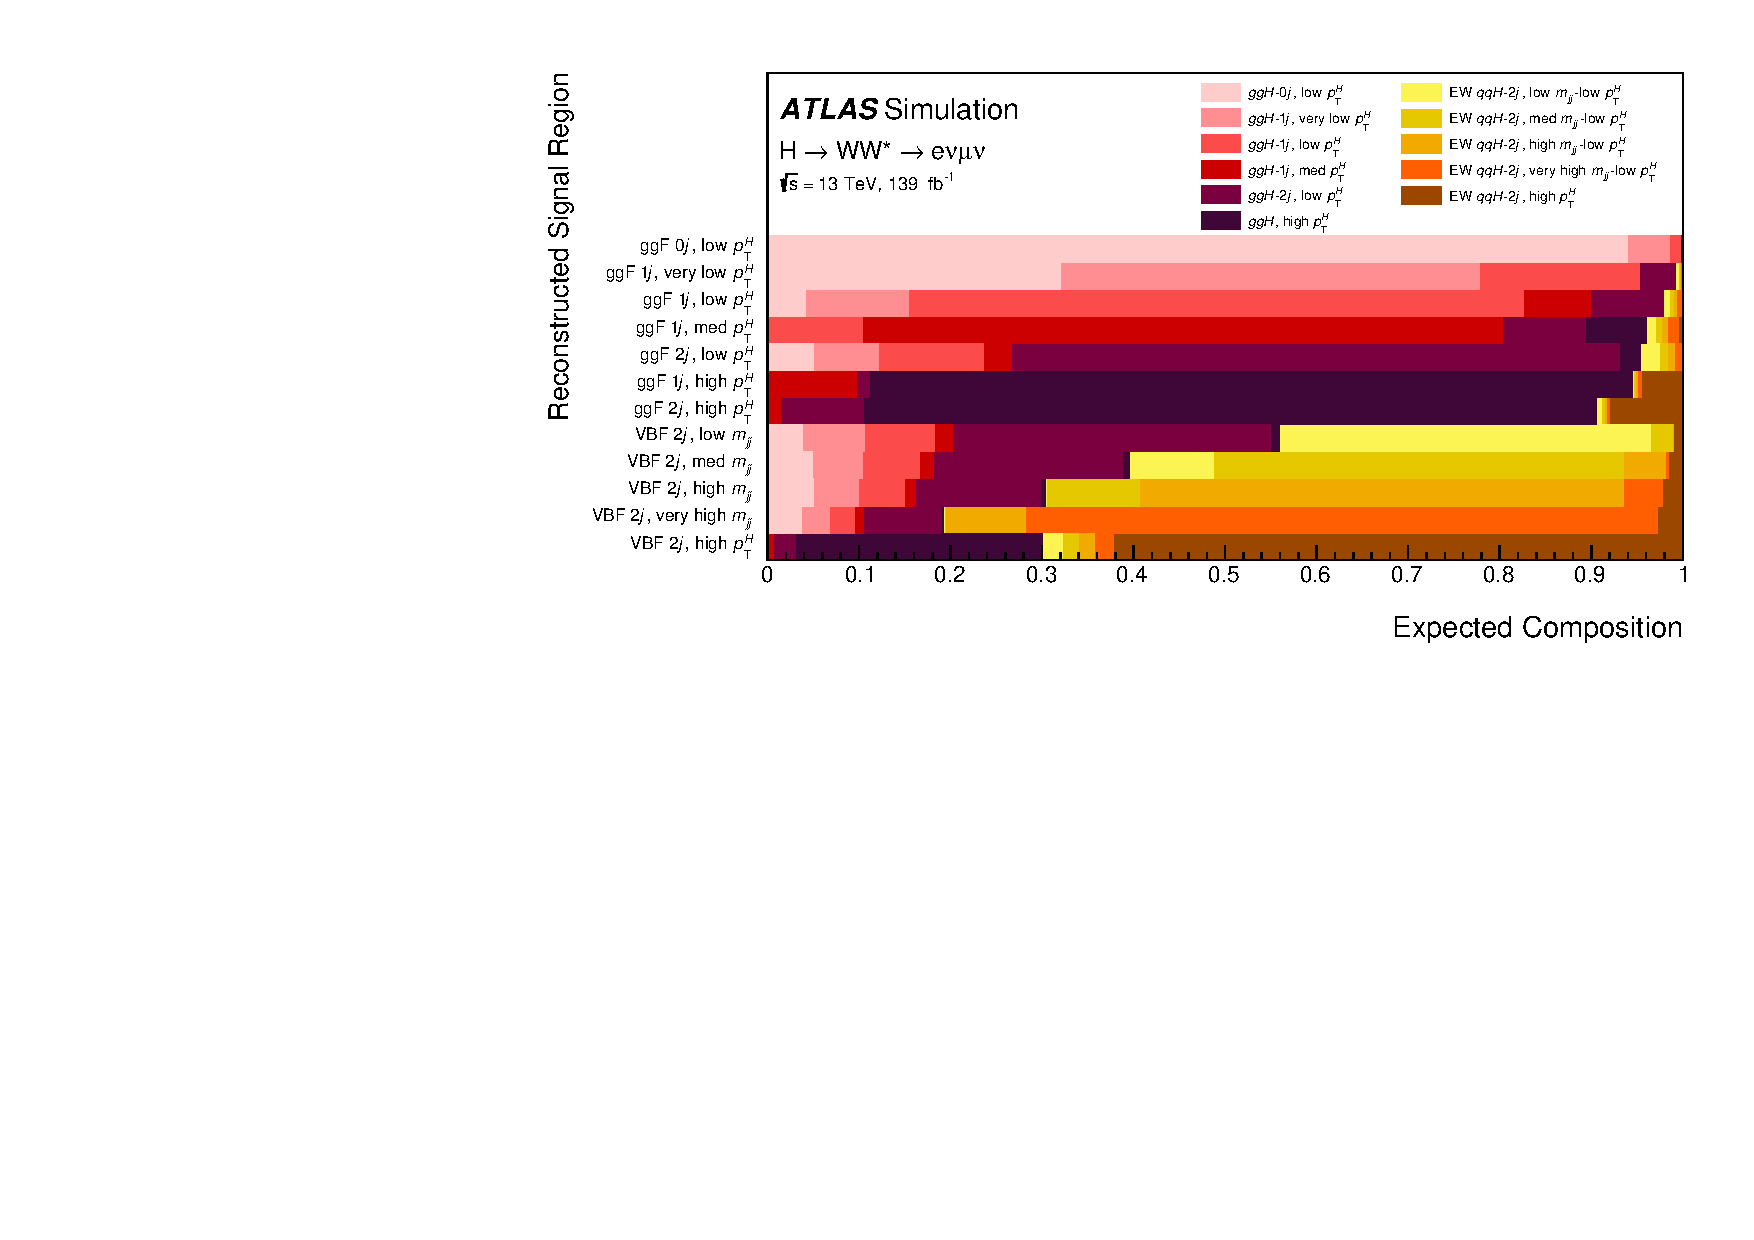
\includegraphics[width=0.90\textwidth]{figures/11-POI/STXS_CompositionMap}
%   \caption{
%     Relative SM signal composition in terms of the measured STXS bin for each reconstructed signal region.
%     \label{fig:STXS_Composition}
%   }
% \end{figure}



\section{Background Estimation}
\label{sec:bkg-estimation}
\todo{Provide table with backgrounds and characteristics...see S Gadatsch thesis Table 5.1 page 126???}

One of the crucial tasks of a physics analysis is to estimate the different background contributions in the SR as accurately as possible.
In this thesis, three different methods are applied for this purpose: 
The top quark, \Zjets, and continuum $WW$ background (not for the VBF category) are estimated using subsidiary measurements in so-called control regions (CRs), processes with misidentified leptons are estimated using a data-driven method known as the \emph{fake factor method}, and all other background contributions are estimated solely based on simulated samples normalised to the theoretical cross sections for the specific processes.
The following provides an overview of the different estimates.

\subsection{Backgrounds estimated with control regions}

- Explain NF method (I guess a formula would be great?)
- Reference table with all selection criteria

\subsubsection{WW}

- Mention mostly selections

\subsubsection{Top}
- Mention mostly selections
\subsubsection{Zjets}
- Mention mostly selections

\subsection{Backgrounds with misidentified leptons}
- Explain fake factor method!

\subsection{Backgrounds estimated with simulated samples}
- Mention validation region
- List xsecs?

\section{Discrimination of the VBF Signal with a Deep Neural Network}
\label{sec:dnn}
%%%%%%%%%%%%%%%%%%%%%%%%%%%%%%%%%%%%%%%%%%%%%%%%%%%%%%%
% Copied from previous \section{Neural Network Training}
The work presented in this thesis uses supervised learning techniques to train a binary classifier that distinguishes between signal-like and background-like events. 
For such a purpose, only a single output node is required, that uses a logistic sigmoid as activation function such that $y = \sigma(x)$, where $\sigma(x)$ is defined as in \cref{eq:logistic-sigmoid}.
The network is trained with simulated $pp$ collision events that have ground-truth labels called \emph{target values} in the following. The target value, $t_n$, for a given event $n$ has a value of $t_n = 1$, if the simulated event is a signal event, and $t_n = 0$ otherwise.

% From PAPER
% DNN that is implemented through Keras [116] and 341 TensorFlow [117],

\subsection{Optimization and performance metrics}
The task at hand is to construct a function that separates the VBF signal process as well as possible from the background processes.
To this end, the cross entropy loss is used as a measure of the separation and the parameters of the neural network model are learned using backpropagation.
In this analysis, the more meaningful measure of the separation is the expected discovery significance (see \cref{chap:statistics}) of the VBF signal process over the background processes. 
It would therefore be natural to directly optimise the discovery significance when training the neural network. 
However, this is not trivial because the loss function must be differentiable with respect to the parameters of the network\footnote{There are attempts to achieve exactly this, as shown in \ccite{ELWOODZ0INML}.} which is not the case for the discovery significance as it is a discrete function of the number of signal and background events. 
In practice, the cross entropy loss is highly anti-correlated with the discovery significance, which is shown in \cref{FIG}.
The training is therefore performed based on the cross entropy loss and the discovery significance is used only to evaluate the trained model. The significance is computed based on the distribution of the output of the neural network. 
% \begin{itemize}
%     \item The cross entropy loss is used during the training to learn the parameters of the neural network. 
%     \item The discovery significance shown in \cref{eq:discovery-significance} is used as an evaluation metric of a trained model.
%     \item Information about systematic uncertainties is included in the discovery significance to perform the final optimisation and choose the neural network. 
% \end{itemize}

% The training of the neural network itself, however, uses the cross entropy loss function to learn the optimal parameters. This function must be differentiable with respect to the parameters of the model in order to use backpropagation. 
% Therefore, it is not trivial to use the discovery significance in the training of the neural network itself.
% The parameters of the neural network are learned by using backpropagation to minimize the cross entropy loss. 

% The task at hand is to construct a function that separates signal processes as well as possible from background processes, based on the statistical significance of the signal process over the background processes.

% During the training of the neural network, a differentiable loss function is required in order to perform backpropagation.
% The loss function must be fully differentiable with respect to the parameters of the model in order to perform gradient descent optimisation.
% This requires the definition of a metric that can be optimised to achieve exactly this. 
% For binary classification, the cross entropy loss is the most common choice and also used in this analysis during the training.
% FROM ARTICLE
% parameters learned by the model are determined by minimizing a chosen loss function.
% - optimization during training: needs to be differentiable w.r.t. network parameters  -> loss function
% - ultimate figure of merit: likelihood fit
% - technically unfeasible
% - simple significance can be used
% - simple significance with added uncertainties!
% -> show that it is highly correlated with the loss function of the network
% - Plot with loss vs significance

\subsection{Training optimization}

multidimensional optimization problem:
ML related
- network architecture
- learning rate (batch size)
- optimizer
- regularization technique
- choice of k-fold method
Physics related
- set of input features (observables)
- weights corresponding to different processes in training data set



- Historical developments, features freezes, limitations of computing resources/turnaround time

- Flow chart for historical strategy:

Fixed: batchsize, reLU activation, sigmoid as output activation, cross-entropy loss

STAGE 1 OPTIMIZATION (FOM: simple significance, 80/20 split)
Temporary: regularisation, adagrad (adaptive learning rate! (no need to overoptimize it)), architecture
-> Choose input variables. 

Fixed: batchsize, input features

STAGE 2 OPTIMIZATION (FOM: simple significance, 80/20 split)
-> Test optimizer -> Adagrad is good
-> Test different architectures -> A larger one was better
-> Double-check regularisation -> adjust dropout

Fixed: batchsize, input features, optimizer, architecture, regularisation

STAGE 3 OPTIMIZATION (FOM: simple significance including systematics!, k-fold)
-> Choice of k-fold: try to go higher than 5-fold. No favorable results and more bookkeeping, keep 5-fold
-> Physics weights optimization (always scanning learning rate) -> choose weights!

Fixed: Everything


Model choice: Choose model with highest significance in validation set!
Model validation: Validate model comparing against test set!


% \subsubsection{Neural network hyperparameter optimization}
% %\subsection{Prospect Studies for Common VBF and ggF HWW 2-jet Analysis with Multiclass Classification}
% ML related
% - network architecture
% - learning rate (batch size)
% - optimizer
% - regularization technique
% - choice of k-fold method
% \subsubsection{Physics input optimization}
% Physics related
% - set of input features (observables)
% - weights corresponding to different processes in training data set


\subsection{Final model validation}
- compare distribution of different subsets to double-check for overtraining


\FloatBarrier
\section{Systematic Uncertainties}
\label{sec:systematics}
This analysis is affected by several sources of systematic uncertainties.
They can be grouped into \emph{experimental uncertainties} and \emph{theoretical uncertainties}.
The experimental uncertainties are related to the detector performance and associated to the identification, reconstruction, and trigger efficiencies, as well as the limited knowledge of the scale and resolution of energy and momentum measurements.
The theoretical uncertainties for both the signal and background processes arise from the assumptions made in the MC simulations as well as theoretical cross-section calculations. 
% In a multi-category analysis, the sign and magnitude of these experimental uncertainties are calculated separately in each category.
All uncertainties are taken into account by constructing respective varied MC templates of the statistical model and using them to define the corresponding nuisance parameters, as described in \cref{chap:statistics}.

\subsection{Experimental uncertainties}
Experimental uncertainties are typically derived in separate calibration measurements, each of which provides a set of sometimes many sources of uncertainty to be considered in physical analyses.
For example, the uncertainties related to the jet energy resolution arise from different sources such as pile-up conditions, method non-closures, etc., which is explained in detail in \cref{chap:calibration}.
% More details on the uncertainties related to jets, in particular the jet energy resolution, are provided in \cref{chap:calibration}. 
In the statistical analysis, the experimental uncertainties are constraint in the likelihood by Gaussians with widths corresponding to the derived nominal uncertainties.
The experimental uncertainties can be further divided into uncertainties affecting the entire event, referred to as \emph{scale-factor} (SF) uncertainties, and uncertainties specific to individual physics objects, referred to as \emph{four-vector} (P4) uncertainties.
While the former is applied to the events as a flat scale factor and thus cannot change the shape of the final discriminant, the latter can cause events to migrate between different histogram bins and thus induce a shape difference between the nominal and the varied template.
A complete list of experimental uncertainties considered is provided in \cref{tab:exp-uncertainties}, including references to the relevant calibration measurements. 

% From MASTER thesis:
% Experimental uncertainties are usually derived externally by dedicated calibration measurements, based on actual data measurements. The constraint terms for the introduced nuisance parameters are represented by Gaussians with a width of the provided nominal uncertainty. Since the subsidiary measurements are generally based on many events, this assumption is supported by the central limit theorem.
Additionally, the uncertainties associated to the background with misidentified leptons are considered as experimental uncertainties. They enter via the uncertainties derived for the fake factors, as explained in \cref{subsec:misid-bkg}, and thus only impact the normalisation of the statistical templates. They are discussed in \cref{subsec:misid-bkg}.
\TDinote{}{Maybe provide more info to exp uncertainties}
\TDinote{}{At least do one thing and refer to JER uncertainties!}
% NOT SURE IF I SHOULD DO THE FOLLOWING! START WITHOUT, maybe reconsider
% - Discuss some of the largest SHAPE uncertainties in VBF? 
%     -> I studied it quite a bit so could definitely add some content. 
%     -> In results section?
% A review of all the values of the uncertainties would go beyond the scope of this thesis and luckily many of them are negligible for the final results. The following highlights the most important experimental uncertainties for the VBF analysis, to which the author of this thesis contributed. 
% QUESTIONS:
% - Mention NP names!?
% Ralf's thesis: Nope
% Carsten's thesis: Yep
% Hannah Arnold: Yep
% Dickinson: Nope and very short. Includes 'constraint type' when mentioning systematics
% From paper:
% The largest sources of experimental uncertainties affecting the ggF measurement are from the 푏-jet 517 identification, the pile-up modelling, the jet energy resolution, and the Mis-Id background estimate. For the 518 VBF measurement, the largest source of experimental uncertainty comes from the 퐸miss T reconstruction.
\begin{table}[ht]
    \begin{center}
        \begin{tabular}{l c c}
    \toprule
    Source & Number of NPs & Type \\
    \midrule
    \textbf{Event} & & \\
    \midrule
    Luminosity \cite{ATLAS-CONF-2019-021} & 1 & SF \\
    Pileup reweighting & 1 & SF \\
    \midrule
    \textbf{Electrons} \cite{EGAM-2018-01} & & \\
    \midrule
    Trigger \cite{TRIG-2018-05} & 1 & SF \\
    Reconstruction & 1 & SF \\
    Identification & 35 & SF \\
    Isolation & 1 & SF \\
    Energy scale & 1 & P4 \\
    Energy resolution & 1 & P4 \\
    \midrule
    \textbf{Muons} \cite{MUON-2018-03} & &  \\
    \midrule
    Trigger \cite{TRIG-2018-01} & 2 & SF \\
    Reconstruction & 2 & SF \\
    %Identification & 2 \\
    Track-to-vertex association & 2 & SF \\
    Isolation & 2 & SF \\
    Energy scale & 3 & P4 \\
    Energy resolution & 2 & P4 \\
    \midrule
    \textbf{Jets} \cite{JETM-2018-05} & & \\
    \midrule
    Energy scale (JES) & 28 & P4 \\
    Energy resolution (JER) & 13 & P4\\
    JVT efficiency \cite{ATLAS-CONF-2014-018} & 1 & SF \\
    $b$-tagging \cite{FTAG-2018-01} & 12 & SF \\
    \midrule
    \pmb{$E_{\rm T}^{\mathrm{miss}}$} \cite{PERF-2016-07} & & \\
    \midrule
    Energy scale of soft term & 2 & P4 \\
    Energy resolution of soft term & 2 & P4 \\
    \bottomrule
\end{tabular}

    \end{center}
    \caption{Summary of experimental uncertainties considered, including their total number of nuisance parameters (NPs) and a specification whether they represent scale-factor (SF) uncertainties or four-vector (P4) uncertainties.
    }
    \label{tab:exp-uncertainties}
\end{table}



\subsection{Theoretical uncertainties}
The nominal MC simulations for both the signal and background processes rely on a set of assumptions that must be made because of the imprecise knowledge of various effects. Assumptions include the choice of renormalisation and factorisation scale, the choice of PDFs, the value of experimentally measured parameters like $\alpha_s$, or assumptions about non-perturbative effects such as the parton showering, hadronisation, and underlying event model. 
The uncertainties arising from such assumptions are determined either by directly varying parameters within the nominal MC simulation and comparing the predictions, or by comparing the nominal predictions with alternative simulations. 
The uncertainties can affect both the overall normalisation of the signal and background processes and the shape of the final discriminant.  
% Imprecise knowledge of the parton showering process and underlying event, missing higher order calculations, and uncertainties in the strong coupling constant $\alpha_s$ as well as the PDFs. In some cases, further process-specific uncertainties are taken into account.
% - Derived by 
% - Affect normalisation and shape of final discriminant

\subsubsection{Signal uncertainties}
Uncertainties affecting the signal processes can be separated into two types: uncertainties that only affect the predicted SM cross section and thus only impact the overall normalisation of the process, and uncertainties arising from the acceptance effects due to the limited detector coverage or analysis selections. The latter can also impact the shape of the final discriminants. 
In the case of cross-section measurements, the first type of uncertainties are factored out and not included in the statistical model. For signal strength measurement both uncertainty components are included. 

For both the ggF and VBF signal process, the uncertainties are estimated that arise from the choice of PDF, including the uncertainties on $\alpha_s$, the choice of parton shower model, and matrix element matching.
The PDF uncertainty is estimated by taken the standard deviation of in total 30 independent Hessian-reduced error sets corresponding to the PDFLHC15 set \cite{Butterworth:2015oua}. 
The parton shower and matrix element matching uncertainty is derived from the sample comparisons indicated in \cref{tab:mcsamples}.
Cross-section uncertainties arising from both missing higher-order contributions in the cross-section calculations and migration effects on the ggF cross sections in different \Njets categories are estimated according to the descriptions provided in \ccite{deFlorian:2016spz,Stewart:2011cf,Stewart:2013faa,Liu:2013hba,Boughezal:2013oha,Gangal:2013nxa}.
This includes uncertainties from the choice of factorization and renormalization scales, the choice of resummation scales, and the ggF migrations between the \ZeroJet and \OneJet regions or between the $N_{\text{jet}} \ge 1$  and \TwoJet categories.
For the ggF migration uncertainties in the \TwoJet categories the so-called Steward Tackmann procedure is used, where the inclusive cross sections in categories $N_{\text{jet}} \ge N$ and $N_{\text{jet}} \ge N+1$ are assumed to be independent and therefore the uncertainty on the exclusive cross section in the $N_{\text{jet}} = N$ can be estimated by the sum in quadrature of the uncertainties of the inclusive cross sections.
%OR THIS: where uncertainties in exclusive jet bins are estimated based on scale variations in inclusive bins.



\paragraph{STXS signal uncertainties}
% Same uncertainties but for each truth bin:
% ONLY cross-section uncertainties, from INT NOTE: As such, the samples or weight variations used to evaluate the signal uncertainties 2509 must be normalized to the same cross-section at truth-level in each STXS bin, prior to examining their 2510 effects on the yield in signal region. 
\TDinote{}{To be included}


% From paper
%For signal processes, the approach described in Refs. [11, 124] is used for estimating the variations due 528 to the impact of higher-order contributions not included in the calculations and migration effects on the 529 푁jet ggF cross sections. In particular, the uncertainty from the choice of factorization and renormalization 530 scales, the choice of resummation scales, and the ggF migrations between the 0-jet and 1-jet phase-space 531 bins or between the 1-jet and ≥ 2-jet bins are considered [11, 125–128].
%from renormalization and factorization scale choices (known as \emph{QCD scale} uncertainties),

% Dickinson
% Uncertainties on the predicted Standard Model cross section of process p are not included on the measurement of cross section p. However, these uncertainties are included on measurements of the signal strength μp, since this result parameterizes the cross section in terms of the SM prediction. In addition, if a process q 6= p is not measured simultaneously, but is fixed to the SM expectation, then theory uncertainties on the inclusive SM q are included on the measurement of both p and μp.Migrationuncertaintiesareincludedonmeasurements of both p and μp.
\subsubsection{Background uncertainties}
%The following provides an overview of the estimation of the theoretical uncertainties underlying the background predictions. 
% \paragraph{Common uncertainty estimates between background processes}
%The method used to estimate some background uncertainties are common for different processes. 

The uncertainties related to the various background estimates are derived in a similar way as the uncertainties for the signals.  

\paragraph{Common methods} The same methods are used for different processes to derive some of the background uncertainties. 
%Some background uncertainties are estimated with the same methods for different processes. 
%They are referenced in the paragraphs below, that provide specifics on the uncertainties of different processes, and include:
\begin{itemize}
    \item Uncertainties arising from the choice of the nominal renormalisation ($\mu_R^\text{nom}$) and factorisation scales ($\mu_F^\text{nom}$), together denoted \emph{QCD scales}, are estimated using both coherent and incoherent variations $\{\mu^{\text{var}}_R , \mu^{\text{var}}_F \} = \{v_R, v_F \} \times \{\mu^{\text{nom}}_R , \mu^{\text{nom}}_F \}$ with $v_R, v_F = 0.5, 1, 2$ excluding the combinations $\{v_R, v_F \} = \{0.5, 2\}, \{2, 0.5\}$. 
    The maximum of these 7 different variations are taken as the total scale uncertainty.
    %his uncertainty is referred to as \emph{7-point QCD scale} uncertainty.
    \item The uncertainty associated to the choice of using the \nnpdfnnlo (or \nnpdfnlo) ~\cite{Ball:2014uwa} set of PDFs is estimated by the standard deviation of the predictions of 100 \nnpdfnnlo (or \nnpdfnlo) replicas.
    % \begin{equation}
    %     \sigma_{\text{PDF}} = \sqrt{ \frac{1}{99} \sum_{i=1}^{100} \left(  n^\text{var}_i - \mu \right) }
    % % \text{Error}^{R}_{J}(PDF)=\sqrt{\frac{1}{99}\sum_{i=1}^{100}\left(\left.\frac{NSR^R_J}{NCR_J}\right|_i-\left\langle\frac{NSR^R_J}{NCR_J}\right\rangle\right)^2}.
    % \end{equation}
    \item The uncertainty associated to the strong coupling constant, $\alpha_s$, is estimated by taking the symmetrized average of the expected event count when varying $\alpha_s$ up and down, 
     \begin{equation}
        \sigma_{\alpha_s}^\text{up/down} = 1 \pm 0.5 \frac{ \text{max}(N^\text{up},N^\text{down}) - \text{min}(N^\text{up},N^\text{down})}{N^\text{nom}}
        % \text{Error}^{R}_{J}(\alpha_s)=\frac{1}{2}\left[\frac{NSR^R_J(\alpha_s^{\text{high}})}{NCR_J(\alpha_s^{\text{high}})}-\frac{NSR^R_J(\alpha_s^{\text{low}})}{NCR_J(\alpha_s^{\text{low}})}\right].
    \end{equation}
    where $N^\text{nom}$ are the nominally expected yields and $N^\text{up}$ and $N^\text{down}$ are the expected yields when $\alpha_s$ is varied up and down, respectively.
    \item The uncertainty due the choice of the parton shower model is estimated by comparing the nominal MC simulations with an alternative simulation setup as indicated in \cref{tab:mcsamples}. 
    % \item The uncertainty due to the choice of the matching procedure between the matrix element and parton shower is also estimated by comparing the nominal MC simulations with an alternative simulation setup as indicated in \cref{tab:mcsamples}.  
    % \item Shower uncertainty based on comparison between alternative shower models (usually \textsc{Pythia8} vs \textsc{Herwig7}) indicated in \cref{tab:mcsamples}.
    % \item Matching uncertainty based on comparison between different matrix element generators as indicated in \cref{tab:mcsamples}.
\end{itemize}

\noindent The following provides details on the specific uncertainties considered for each background process. 
\paragraph{$qq \to WW$} 
The uncertainties due to the QCD scale choices, the choice of PDF, and $\alpha_s$ are estimated as discussed above.
% Uncertainties due to scale choices are estimated with the 7-point QCD scale uncertainty and the PDF uncertainty with the set of 100 NNPDF3.0NLO replicas as explained above. 
% PDF uncertainties:
% The PDF and $alpha_s$ uncertainties are evaluated from the standard deviation of 100 NNPDF3.0NLO replicas. 
% The PDF replicas and alphahigh,low s are included as alternative weights in the nominal \Sherpa samples.
The uncertainty due to the choice of parton shower model is covered by two separate comparisons based on generator-level samples.
The first accounts for the uncertainty due to the resummation scale choice in the nominal sample that determines the matching of the NLO matrix elements with the parton shower. 
To assess the uncertainty, the resummation scale is varied by a factor of two up and down.
The second comparison varies how the momentum recoil is evaluated in the parton shower provided by the \Sherpa generator. The strategy used in the nominal MC simulation is described in \cite{Hoeche:2009rj}, the alternative approach is detailed in \cite{Schumann:2007mg}. 
The nominal \Sherpa sample uses a cut at $Q=20\,$GeV to separate the phase spaces covered by the matrix element calculations and the parton shower. This scale is arbitrary and the associated uncertainty due to that choice is estimated by varying it up and down such that $Q = 15\,\GeV$ and $Q = 30\,\GeV$. The uncertainty is estimated based on generator-level sample comparisons.
% \todo{Not sure if this is maybe too much detail?}
% \todo{What's the difference between resummation and matching/merging uncertainty?}
% \todo{Introduce abbreviations, QSF, CSSKIN, CKKW?}

% QSF
% - Resummation scale (QSF)
% -> Take larger variation
% % CSSKIN
% - Parton shower recoil scheme

% CKKW
% - Merging scale (CKKW)
% -> Take larger variation
%The QSF, CSSKIN, and CKKW uncertainty are all estimated using generator-level samples.

\paragraph{$gg \to WW$} 
The $gg \to WW$ process contributes around 10\% to the total $WW$ background in most signal regions. The \Sherpa sample used is generated only at leading order precision. For the ggF and VBF \TwoJet categories, a conservative uncertainty of $+100/-50$\% is therefore used. For the ggF \OneJet and \TwoJet categories, the NLO scale uncertainties using the latest theoretical predictions as shown in \ccite{Grazzini_2020} are used.

\paragraph{EW $qq \to WWqq$}
%Uses MadGraph+Pythia8 at reco level with the following uncertainties derived.
The uncertainties from the choice of QCD scales, choice of PDF, and $\alpha_s$ are estimated as described above.
% QCD scale:
%For this LO sample, varying the μR (renormalization) scale has no effect because the ME does not include 2342 any powers of αs, but varying the factorization scale μF is expected to give a conservative uncertainty 2343 band that covers differences between the LO and NLO predictions (see, for example, Figure 3 of [121])
The shower uncertainty is estimated by comparing the nominal \MADGRAPH+\PythiaEight sample with a sample that interfaces \MADGRAPH and \HerwigV{7}.
% Shower
% MadGraph+Pythia8 vs MadGraph+Herwig7 
An additional uncertainty due to the choice of electroweak scale and the missing higher orders are estimated based on the leading-log approximation \cite{Denner_2019}, yielding an additional normalisation uncertainty of $\pm 15$\%. 

% EW scale (alpha)
% Int note: The main effect of missing EW scales is expected to come from the NLO EW correction.
% Paper: he EW 푊푊 process, which contributes most significantly in the highest VBF DNN bin, 538 is assigned an additional normalization uncertainty of 15% due to NLO EW corrections, as calculated 539 using the leading-log approximation [129].

% PDF+alpha_s 
% SAME AS qqWW!
% IntNote: 100 NNPDF replicas around 2335 the nominal. Similarly, the effect of αs was evaluated using three replicas with different settings of αs.


\paragraph{Background with top quarks}
The uncertainties arising from the choice of parton shower model, the choice of QCD scales, and choice of PDF, is estimated as described above. 
% Shower uncertainty
% Powheg+Pythia8 and Powheg+Herwig7
% QCD scale with 7-point envelope
% LIKE qqWW!
% PDF uncertainty with 100 NNPDF3.0 replicas (MISSES ALPHA S!?)
The uncertainty due to the matching procedure between matrix element calculations and the parton shower are estimated by comparing the predictions of MC simulations based on \Powheg+\PythiaEight and \aMCATNLO+\PythiaEight.
% Matching uncertainty
% Int Note: The difference between the prediction of Powheg+Pythia8 and the aMCAtNlo+Pythia8 sample is taken as a matching uncertainty between 
In addition, uncertainties are considered due to additional initial state (ISR) or final state radiation (FSR). The parameters determining the amount of ISR and FSR are varied up and down.
% Initial State Radiation (ISR) and Final State Radiation (FSR)
% -> missing hpdamp factor!?
For the $Wt$ process only, an additional uncertainty is considered due to interference effects between processes with single top quarks and $t\bar{t}$ processes. This uncertainty uses an alternative diagram removal scheme \cite{Frixione:2008yi}. %(DR instead of DS scheme) . 
% Single Top Interference (Wt only)


\paragraph{\Ztautau background}
% QCD scale: 7-point envelope
% LIKE qqWW
The uncertainty due to the choice of QCD scales, the choice of PDF, and  $\alpha_s$ is estimated as described above. 
% PDF: NNPDF3.0 100 NNPDF replicas
% alpha_s: two NNPDF3.0nnlo αs variations.
The nominal \SHERPAV{2.2.1} generator handles the simulation of the matrix element and parton shower with a custom tune. To estimate the uncertainty arising from that choice the nominal sample is compared to a sample generated with \textsc{MadGraph5\_aMC@NLO+Pythia8} and the A14 tune. 

% GENERATOR:
% INT NOTE: \Sherpa 2.2.1 handles simulation of the matrix element and parton shower with a custom tune. Uncertainty 2447 associated with this choice of generator is evaluated by comparing with MadGraph5_aMC@NLO, which 2448 is interfaced to Pythia8 with the A14 tune for modelling of the parton shower and underlying event.

\paragraph{Other backgrounds}
The overall normalisation of the $V\gamma$ sample is assigned an uncertainty of $+100/-50\%$ to account for potential mismodelling of this background. For Other $VV$ and triboson processes, a 12\% uncertainty is applied for similar reasons. 
% Int note: A flat -50%/+100% uncertainty on the overall normalization of V γ processes is applied to account for 2494 potential mismodelling of this background. For Non-WW diboson processes, a 12% normalization 2495 uncertainty is applied. This uncertainty was evaluated for the Z+jets fake factor estimate (section 7.2) 2496 and includes contributions from QCD scale, PDF and αS. This uncertainty is also applied for triboson 2497 processes.



% \subsection{Discussion of most impactful uncertainties}

% - THINK ABOUT ADDING THIS SECTION!
% - MIGHT INDEED BE RELEVANT 
% - COULD ALSO ADD THIS TO THE END OF RESULTS SECTION or an IMPROVEMENTS SECTION



\section{The Statistical Model}
\label{sec:stats-analysis}
% From Hannah Arnold Thesis
% - using the HistFactory tool [326] and the RooStats/ RooFit framework [327, 328].

The VBF and ggF signals are measured using a binned likelihood fit of the MC template to data in the SRs and CRs. The uncertainties are incorporated as NPs in the likelihood. The procedure is explained in detail in \cref{chap:statistics}. 
This section first provides details on the statistical model, including the treatment of uncertainties, and discusses the expected performance and validation of the likelihood fit.

% From nature diff for mu and xsec fit:
% Theory uncertainties on the signal acceptance, i.e.
% 163 fractions of signal events in a detectable kinematic range, are taken into account in the measurements of
% 164 production and decay processes, while uncertainties on signal cross sections and branching fractions are
% 165 additionally taken into account for all other measurements

\subsection{Background templates}
All background processes discussed in \cref{sec:bkg-estimation} are included in the likelihood via the expectation value. 
The normalization of processes for which CRs are defined is controlled by freely floating NFs in the fit. All other processes are normalized to their respective theoretical cross sections including their uncertainties, except the background from misidentified leptons that is estimated in a data-driven method.
In summary, the MC fit template is constructed using the following contributions:
\begin{itemize}
    \item VBF signals, inclusive ($H_{\mathrm{VBF}}$) or split in STXS bins ($H_{\mathrm{EW\,} qqH\mathrm{, i}}$), scaled with signal strengths.
    \item ggF signals, inclusive ($H_{\mathrm{ggF}}$) or split in STXS bins ($H_{ggH\mathrm{, i}}$), scaled with signal strengths.
    \item Other Higgs boson processes (Other $H$).
    \item \ttbar and $Wt$, separately treating uncertainties but using the same NF.
    \item $qq \to WW$ and $gg \to WW$ (together $WW$ (Strong)), separately treating uncertainties and using NFs for the $qq \to WW$ process in the ggF categories.
    \item Electroweak production of $WW$ ($WW$ (EW)).
    \item \Zgamma using NFs.
    \item Misidentified leptons background (Mis-Id).
    \item $V\gamma$, other diboson processes ($W\gamma^*$, $WZ$, $ZZ$), and triboson processes, separately treating uncertainties (collectively denoted \OtherVVV).
\end{itemize}

\subsection{Fit types and inputs}
The signal yields are parametrized as signal strengths in the likelihood, 
\begin{equation}
    \label{eq:incl-ggF-VBF-signal-strengths}
    \mu_{\text{signal}} = \frac{ [ \sigma_{\text{signal}}  \times \BR(H \to WW^*) ]_\text{meas} } { [ \sigma_{\text{signal}} \times \BR(H \to WW^*) ]_\text{SM}}, 
\end{equation}
with the signal definition depending on the type of measurement performed.
The results presented are based on three types of fits:
\begin{itemize}
    \item 2-PoI fit: Measurement of the inclusive VBF and ggF production cross sections by extracting two signal strengths $\mu_{\text{VBF}}$ and $\mu_{\text{ggF}}$ as the \emph{parameter of interests} (PoIs).
    \item 1-PoI fit: Measurement of the combined VBF and ggF production cross section, treating the VBF and ggF signal with a common signal strength $\mu_{\text{VBF+ggF}}$.
    \item 11-PoI fit: Measurement of signal cross sections separated in kinematic regions following the STXS framework. In total 11 signal strengths are measured targeting $ggH$ and EW~$qqH$ production.
\end{itemize}
For all cross-section measurements, only signal acceptance uncertainties are considered in the statistical model. 
To quantify the excess of the VBF signal over the background expectation two 2-PoI fits are performed that also include signal cross-section uncertainties in the signal templates. 
The test statistic shown in \cref{sec:hypothesis-testing} is used for this purpose.

The same fit inputs are used for the 2-PoI fit and 1-PoI. They correspond to the nominal SRs and CRs for the \ZeroJet, \OneJet, and \TwoJet categories as defined in \cref{sec:event-categorization,sec:bkg-estimation} and amount to a total number of 22 regions, 11 SRs and 11 CRs.
For the 11-PoI fit, all STXS SRs and CRs are used as defined in \cref{subsec:STXS-categorization,subsubsec:stxs-crs}, which amounts to a total number of 44 regions, 17 SRs and 27 CRs. 

The final fit discriminant in the ggF SRs is the \mT distribution. The same 6 bins are used in all regions: [0-90, 90-100, 100-110, 110-120, 120-130, 130-$\infty$]. 
All VBF SRs use the DNN observable as final discriminant with 7 bins in the nominal VBF SR and 4 bins in the STXS SRs.
The bin boundaries are found based on the procedure explained in \cref{subsec:performance-metrics} and in the nominal VBF SR are: [0-0.25, 0.25-0.52, 0.52-0.68, 0.68-0.77, 0.77-0.83, 0.83-0.87, 0.87-1.00].
For the STXS measurement, the statistical precision in the SRs is smaller. The binning criteria are therefore relaxed and only require at least 10 (5) signal (background) events. The requirement of the relative statistical uncertainty stays the same and must be smaller than 20\%. In addition, the binning is harmonized between all 5 VBF STXS SRs, yielding bin boundaries: [0-0.5, 0.5, 0.74, 0.74-0.87, 0.87, 1.0]. 
The CRs are encoded as one bin each in the likelihood. 
%The signal cross sections are parametrized as signal strengths in the likelihood and extracted from a simultaneous fit to the data in multiple regions.
%depending on the target of the fit, for example,
% \begin{equation}
%     \label{eq:incl-ggF-VBF-signal-strengths}
%     \mu_{\text{ggF/VBF}} = \frac{ [ \sigma_{\text{ggF/VBF}}  \times \BR(H \to WW^*) ]_\text{meas} } { [ \sigma_{\text{ggF/VBF}} \times \BR(H \to WW^*) ]_\text{SM}},
% \end{equation}
% For the measurement of the inclusive ggF and VBF production cross sections a fit is performed to all nominal SRs and CRs in the \ZeroJet, \OneJet, and \TwoJet categories, as defined in \cref{sec:event-categorization,sec:bkg-estimation}. 
% The ggF and VBF cross sections are parametrized as shown in \cref{eq:incl-ggF-VBF-signal-strengths} and treated as the two unconstrained PoIs $\mu_{\text{VBF}}$ and $\mu_{\text{ggF}}$. 
% The same regions are used for the measurement of the combined ggF and VBF cross section, using a single PoI, $\mu_{\text{VBF+ggF}}$, to scale the ggF and VBF yields. 
% For the measurement of 11 STXS cross sections, all STXS SRs and CRs are used as defined in \cref{subsec:STXS-categorization,subsubsec:stxs-crs}. The total number of regions amounts to 44 regions, 17 SRs and 27 CRs. 
% From Paper
%The cross sections for the ggF and VBF production modes are determined in a simultaneous fit to all 574 nominal SRs and CRs in the 푁jet = 0, 푁jet = 1, and 푁jet ≥ 2 categories. The ggF and VBF cross sections are 575 the two unconstrained POIs in this fit. 
%A second fit is performed using these same regions, but measuring a 576 single POI for the combined ggF and VBF yield.
%In both fits, the other Higgs production modes are fixed 577 to their expected yields. 
%A third fit is made to all the STXS regions, where the 11 cross sections measured 578 are POIs. No nuisance parameters are significantly pulled or constrained in any of the fits.

\subsection{Treatment of uncertainties}
The sources of systematic uncertainties are discussed in \cref{sec:stats-analysis}. 
Most uncertainties are fully correlated between the SRs and CRs in all analysis categories. Only the theoretical uncertainties affecting the backgrounds are uncorrelated between the four different categories. The same is true for the NFs. This is a conservative approach and ensures that potential mismodellings observed in one of the categories do not impact other categories. 
Different uncertainties are treated differently in the fit, and before the fit is performed, the uncertainties are scrutinized and possibly preprocessed depending on their type and size using the techniques explained below.

\paragraph{Transfer of uncertainties}
% From INT note
In some regions the available statistical power is not sufficient to correctly estimate the uncertainties. 
In these cases, the uncertainty is evaluated in a more inclusive selection and then applied to the individual smaller regions. This is useful especially for the regions used in the STXS measurement. The specific inclusive region is chosen and only used if the uncertainty derived in the inclusive region is statistically compatible with the uncertainties in the individual regions. 

\paragraph{Pruning and symmetrizing of uncertainties}
Only a few of the systematic uncertainties derived have a significant variation with respect to the nominal MC template. To increase the numerical stability of the fit and reduce the time it takes for the fit to converge, uncertainties are pruned from the likelihood if they do not satisfy certain threshold conditions.
For each NP, the normalization and shape components are pruned independently of each other.
The following cases result in an uncertainty for a given sample being pruned from a region:
\begin{itemize}
    \item A normalization uncertainty is smaller than 0.5\%.
    \item A four-vector normalization uncertainty is smaller than 20\% of the statistical uncertainty. 
    \item A shape uncertainty has no significant slope ($p$-value $< 0.05$).
\end{itemize}
The nominal or alternative samples that have only small yields often lead to large, unphysical variations, due to statistical fluctuations. 
Therefore, a normalization uncertainty is also pruned if it is larger than 80\%. 
This criterion is carefully monitored to ensure that no meaningful uncertainty is pruned.
In addition, some experimental four-momentum uncertainties and uncertainties on STXS signal samples are pruned manually if they are not identified by the above criteria but are clearly dominated by statistical fluctuations and thus deemed unphysical.
Furthermore, the shape component of uncertainties of minor backgrounds ($V\gamma$, \Zgamma) are pruned, mainly because meaningful shape uncertainties cannot be estimated with the available MC samples. 

Statistical fluctuations can also cause the up and down variations to be asymmetric around the nominal value. 
For normalization uncertainties whose up and down variations differ by a factor of two or have the same sign, the larger variation is fixed and also used as ``opposite'' variation by symmetrizing it with respect to nominal.
Similarly, for shape uncertainties that have at least one bin where the up and down variations have the same sign, the full shape uncertainty is symmetrized by fixing the larger variation and symmetrizing it with respect to nominal.

\paragraph{Smoothing of shape uncertainties}
For the DNN discriminant, a smoothing procedure is applied to background shape uncertainties whose estimates are subject to large statistical fluctuations. 
The smoothing procedure is based on a bin merging strategy together with the 353QH running median algorithm~\cite{Friedman353QH}. 
An example of an uncertainty processed in such a way is shown in \cref{fig:dnn:smoothing}.

\begin{figure}[h!]
    \centering
    % \subfloat[]
    %     {
        \newImageResizeCustom{0.6}{figures/plots/shape-uncertainty/ttbar-matching-smoothed.pdf}
        % }
        % \subfloat[]
        % {
        %     \newImageResizeCustom{0.48}{figures/plots/CKKW-smooth.pdf}
        % }
    {\caption[DNN output distribution for the nominal and an alternative \ttbar sample.]{DNN output distribution for the nominal \ttbar sample (\Powheg+\PYTHIA[8]), an alternative sample (\aMCATNLO+\PYTHIA[8]) including the symmetrized distribution with respect to the nominal, and smoothed distributions based on the difference between the nominal and the alternative sample. The alternative sample is used to estimate the uncertainty due to the choice of matching procedure between matrix element calculations and the parton shower. The smoothed distribution is used in the statistical analysis to define the nuisance parameter. More information on the smoothing procedure can be found in the text.
    \label{fig:dnn:smoothing} }}
\end{figure}

\subsection{Expected performance and validation of the likelihood fit}
\label{subsec:expected-performannce}
The analysis strategy is optimized on MC simulated samples, and signal-like data events are only analyzed after the statistical model is validated.
An \emph{Asimov} dataset~\cite{Cowan:2010js} can be used to evaluate the expected performance of the likelihood fit. It is generated under the SM assumption, i.e., assuming the expected values for the backgrounds and signals ($\mu=1$). 
This implies that the values of all fit parameters obtained from a fit (\emph{post-fit} values) to the Asimov dataset correspond to their expected values. 
The Asimov dataset is used to extract the expected uncertainties on the cross-section measurements and to assess the impact of different sources of uncertainties on the final results. 
\Cref{fig:fit:breakdown} shows a representative list of NPs and their influence on the VBF cross section, \sigmaVBF. 

The uncertainties that include ``ATLAS'' in their names correspond to experimental uncertainties, all other uncertainties are related to theory. 
% The NPs are ordered in terms of their contribution to the total uncertainty (\emph{breakdown}) on the cross section \sigmaVBF. 
%The impact is calculated by taking the square root of the difference in quadrature of the uncertainty on $\mu_{\mathrm{VBF}}$ resulting from a fit performed with all parameters floating and a fit where the NP under investigation is fixed to its nominal value. 
It becomes apparent that theoretical uncertainties dominate, in particular the signal modelling uncertainties from the choice of both the parton shower model and the matching procedure between the matrix element and parton shower. 
The largest background uncertainty is from the choice of \ttbar matching procedure and the leading experimental uncertainties come from the effect of the \MET soft term on the resolution of the \MET observable.  
%, resulting from large shape differences in the DNN discriminant when the \MET soft term is varied. 
All said uncertainties are mainly caused by shape differences in the DNN discriminant when the respective source of uncertainty is varied.
The post-fit uncertainties of the NPs relative to their nominal ones are also shown. The \emph{constraints}, i.e., the extent to which the post-fit uncertainty is smaller than the nominal uncertainty, are reasonably small.
This shows that the uncertainties are represented adequately in the statistical model. 
%The expected total uncertainty on the cross-section measurement corresponds to $\Delta \sigmaVBF = \pm  $. 
The expected signal strength is extracted to be $\muVBF = 1^{+0.24}_{-0.21}$.
The expected discovery significance of the VBF signal is $6.2\,\sigma$. 

\Cref{fig:fit:breakdown} also includes the NPs obtained from a fit to the full \RunTwo dataset of the LHC. 
The \emph{pulls} of the NPs, defined as the difference of the post-fit central values and their corresponding nominal ones, $(\hat{\theta} - \theta_0 ) / \Delta \theta_0$, are relatively small. 
Furthermore, the constraints and the breakdown of uncertainties are comparable for the results obtained from a fit to Asimov data and actual data. 
Because of these findings, the statistical model is deemed appropriate for the measurement performed. 
Similar validation studies have been conducted for the ggF cross-section measurement as well as the STXS measurement and lead to the same conclusions. 

\begin{figure}[t]
    \centering
        \newImageResizeCustom{0.65}{figures/plots/breakdown/breakdown_muVBF.pdf}
    {\caption[Contribution of individual NPs to the total uncertainty of $\sigma_{\mathrm{VBF}}$ as well as NP pulls and constraints.]{Contribution of individual NPs to the total uncertainty of the cross section $\sigma_{\mathrm{VBF}}$ relative to the measured value, shown for (green hashed area) the fit to observed data and (orange solid area) the Asimov dataset in the measurement of the inclusive \muVBF and \muGGF cross sections. The leading 20 NPs are shown in decreasing order of their impact (top x-axis).
    The uncertainty due to a single NP is computed by taking the square root of the difference in quadrature of the uncertainties on $\sigma_{\mathrm{VBF}}$ resulting from a fit performed with all parameters free-floating and a fit where the respective NP is fixed to its nominal value. 
    %The impact of a given NP is derived by comparing the uncertainty on $\mu$ resulting from a fully unconditional fit and a fit with the respective NP fixed to its nominal value. The comparison is based on the square root of the difference in quadrature of the two post-fit uncertainties on $\mu$. 
    The dots indicate the pull (bottom x-axis), i.e. the post-fit values of the NPs, $\hat{\theta}$, relative to their nominal values, $\theta_0$. 
    The associated error bars show the post-fit uncertainties of the NPs relative to their nominal uncertainties. 
    The pull is zero by definition for the fit to the Asimov dataset.
% (b): Breakdown
% of the contribution of groups of NPs to the uncertainty on the V H
% PoI. The sum in quadrature of the individual contributions differs
% from the total uncertainty due to correlations between the NPs. Both
% Figures are obtained from a (1+1)-PoI fit. Published in Ref. [5].
    \label{fig:fit:breakdown} }}
\end{figure}
\clearpage
% A listing of the results for the individual parameters obtained in the fit is shown in Fig. 4.25. The total uncertainty has been broken down to the impacts of each individual nuisance parameter (and for certain groups of nuisance parameters). Shown are the breakdowns for the fit to the observed data, as well as for a control fit to an Asimov data set generated with the assumption of μ = 1. The postfit values and uncertainties of the individual nuisance parameters are shown as well, where the constrained nuisance parameters have been normalized to their respective constraints.

% Combination:
% From nature:
% The statistical analysis of the data relies on a likelihood formalism, where the likelihood functions describing each of the input measurements are multiplied to obtain a combined likelihood. The observed yield in each category of reconstructed events follows a Poisson distribution whose parameter is the sum of the predicted signal and background contributions. The predicted signal yield is split into the different production and decay processes, so it can be parameterized as a function of dedicated parameters of interest depending on the tested model.




\FloatBarrier
\section{Results}
\label{sec:hww-results}
This section presents the results of the \HWW\ analysis obtained from fits to data. 

\subsection{Inclusive cross-section measurements}
The ggF and VBF production cross sections times branching fraction are simultaneously measured to be
% Observed XSec
%{\mediumsize
\begin{gather}
\scalebox{0.96}{$
\begin{align*}
  %the 12.0 is a 19.98
  \sigma_{\mathrm{ggF}} \cdot \mathcal{B}_{H \to WW^{\ast}} &= 12.0 \pm 1.4~\mathrm{pb} \\
  &= 12.0 \pm 0.6\;(\mathrm{stat.}) ^{+0.9}_{-0.8}\;(\mathrm{exp.~syst.})\;^{+0.6}_{-0.5}\;(\mathrm{sig.~theo.})\; \pm 0.8~(\mathrm{bkg.~theo.})~\mathrm{pb} \\
  \sigma_{\mathrm{VBF}} \cdot \mathcal{B}_{H \to WW^{\ast}} &= 0.75\;^{+0.19}_{-0.16}~\mathrm{pb} \\
  &= 0.75 \pm 0.11\;(\mathrm{stat.})\;^{+0.07}_{-0.06}\;(\mathrm{exp.~syst.})\;^{+0.12}_{-0.08}\;(\mathrm{sig.~theo.})\;^{+0.07}_{-0.06}\;(\mathrm{bkg.~theo.})~\mathrm{pb},
\end{align*}
$}
\end{gather}
%}
which is consistent with the SM prediction of $10.4\pm 0.5$~pb and $0.81\pm 0.02$~pb for ggF and VBF~\cite{deFlorian:2016spz}, respectively.
\Cref{fig:LL2D} shows the two-dimensional likelihood contour obtained from performing the 2-PoI fit with different fixed values of \muGGF and \muVBF.
\begin{figure}[ht]
  \centering
  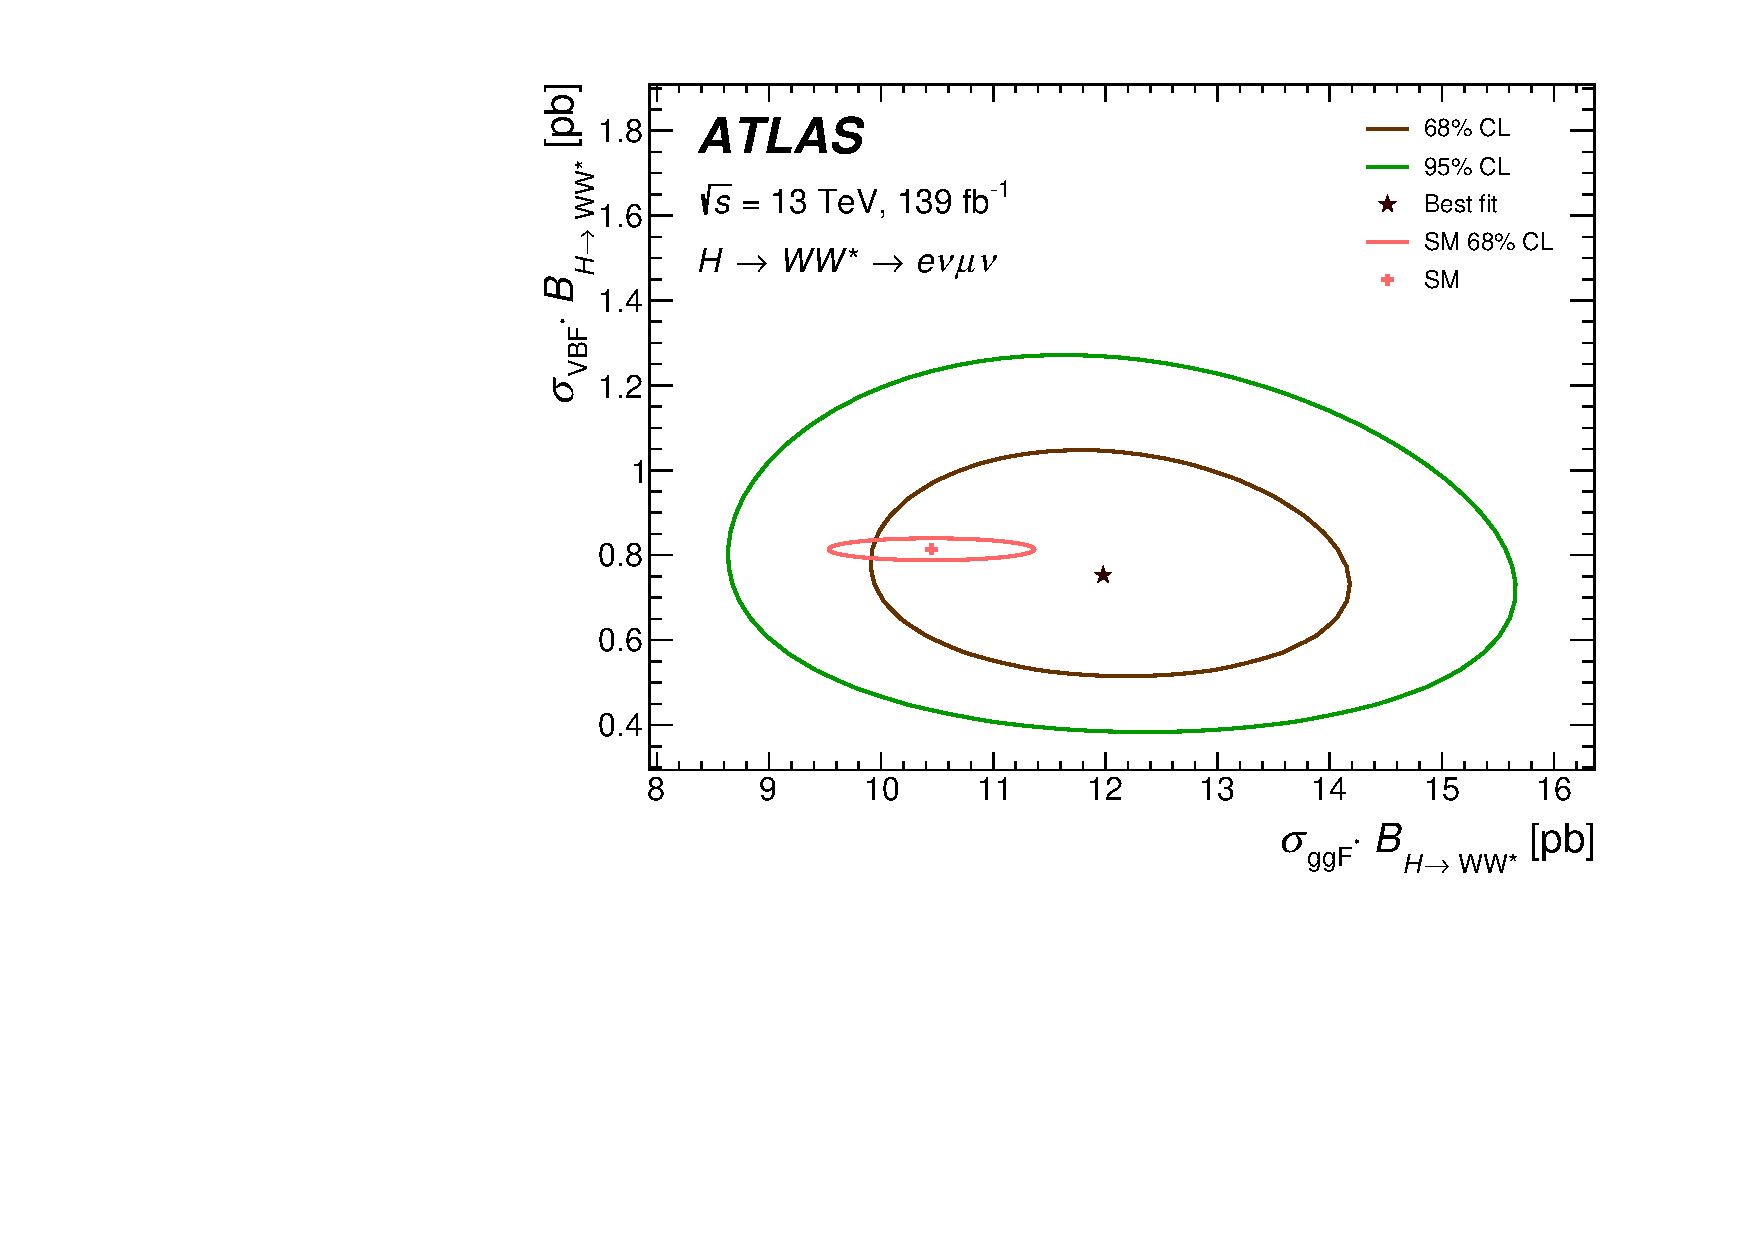
\includegraphics[width=0.75\textwidth]{\paperfiguredir/2-POI/ggF_VBF_likelihood_contour_XSec}
  \caption{
    68\% and 95\% confidence level (CL) two-dimensional contours of $\sigma_{\mathrm{ggF}} \cdot \mathcal{B}_{\hww}$ versus \mbox{$\sigma_{\mathrm{VBF}}\cdot\mathcal{B}_{\hww}$}, compared to the SM prediction shown by the red marker.
    The 68\% CL contour for the SM predictions of the ggF and VBF cross sections times branching fraction~\cite{deFlorian:2016spz} is indicated by the red ellipse.
    Figure and caption taken from \ccite{HWWPaper}.
    \label{fig:LL2D}
  }
\end{figure}
The SM expectation lies well within the 68\% and 95\% confidence level contours.

The 1-PoI fit results in a measurement of the combined ggF and VBF production cross section times branching fraction of
\begin{gather}
  \scalebox{0.94}{$  
\begin{align*}
  \sigma_{\mathrm{ggF+VBF}} \cdot \mathcal{B}_{H \to WW^{\ast}} &= 12.3 \pm 1.3~\mathrm{pb} \\
  &= 12.3 \pm 0.6\;(\mathrm{stat.})\;^{+0.8}_{-0.7}\;(\mathrm{exp.\ syst.})\;\pm 0.6\;(\mathrm{sig.\ theo.})\;\pm 0.7\;(\mathrm{bkg.\ theo.})~\mathrm{pb},
\end{align*}$}
\end{gather}
where $11.3\pm 0.5$~pb are expected from the SM predictions.
\Cref{fig:couplings-POIs} summarizes the results of the inclusive cross-section measurements by presenting the ratio of the measured cross sections divided by the corresponding value predicted by the SM.
\begin{figure}[htb]
  \centering
    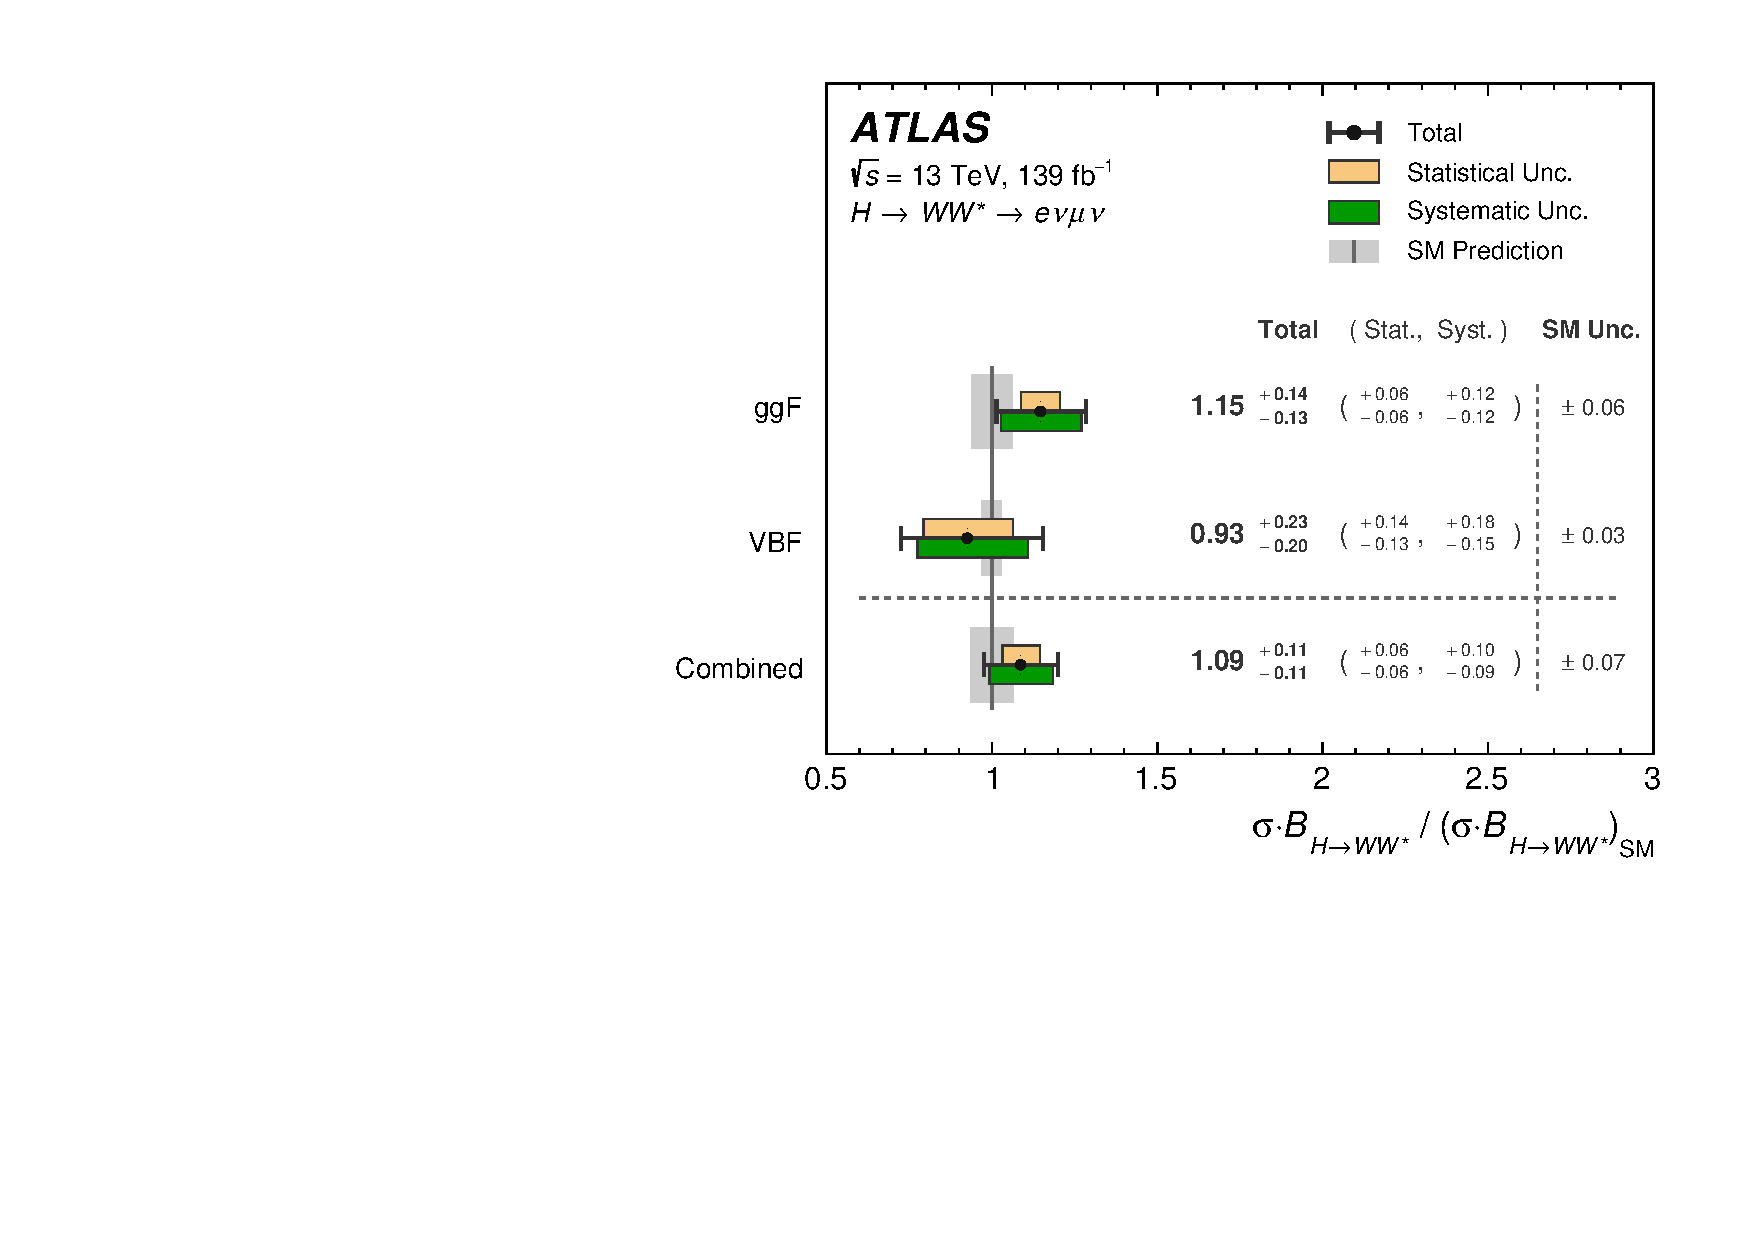
\includegraphics[width=0.8\textwidth]{\paperfiguredir/plot-combined-couplings-pois-xsecs-GreenTan-vert}
    \caption{
      Best-fit values and uncertainties of the $\hww$ cross section for the ggF and VBF processes and their combination, normalized to the corresponding SM prediction.
      The black error bars, green boxes and tan boxes show the total, systematic, and statistical uncertainties in the measurements, respectively.
      The gray bands represent the theory uncertainty of the corresponding Higgs production mode.
      Figure and caption taken from \ccite{HWWPaper}.
      \label{fig:couplings-POIs}
    }
\end{figure}

The uncertainties broken down into several components for the inclusive cross section measurements are shown in \cref{tab:UncertaintyBreakdown_2-POI}. 
The systematic uncertainties dominate the measurements. 
For the ggF measurement, the theoretical uncertainties are of similar size as the experimental uncertainties.
The VBF measurement is dominated by theory uncertainties, in particular VBF signal modelling uncertainties.
The latter is mainly caused by uncertainties related to the modelling of potential jets in addition to the two leading jets, manifesting itself in a large uncertainty due to the choice of parton shower model (see also \cref{subsec:expected-performannce}). The largest contributions from the backgrounds are from uncertainties due to the modelling of top-quark processes, $WW$ production, and the ggF process that can be considered a background in the VBF measurement. 

\begin{table}[ht]
  \centering
  \caption{
    Breakdown of the main contributions to the total uncertainty in $\sigma_{\mathrm{ggF+VBF}} \cdot \mathcal{B}_{\hww}$, $\sigma_{\mathrm{ggF}} \cdot \mathcal{B}_{\hww}$, and $\sigma_{\mathrm{VBF}} \cdot \mathcal{B}_{\hww}$, relative to the measured value.
    The individual sources of systematic uncertainties are grouped together.
    The sum in quadrature of the individual components differs from the total uncertainty due to correlations between the components.
    Table and caption taken from \ccite{HWWPaper}.
  }
  \resizebox{\textwidth}{!}{
    \begin{tabular}{lrrr}
    \toprule
    \noalign{\vskip 1mm}
    % Source          & $\Delta\sigma_{\mathrm{ggF}} \cdot \mathcal{B}_{\hww}$ $[\%]$  & $\Delta\sigma_{\mathrm{VBF}} \cdot \mathcal{B}_{\hww}$ $[\%]$  \\
    Source                              & $\frac{\Delta\sigma_{\mathrm{ggF+VBF}} \cdot \mathcal{B}_{\hww}}{\sigma_{\mathrm{ggF+VBF}} \cdot \mathcal{B}_{\hww}}$ $[\%]$ & $\frac{\Delta\sigma_{\mathrm{ggF}} \cdot \mathcal{B}_{\hww}}{\sigma_{\mathrm{ggF}} \cdot \mathcal{B}_{\hww}}$ $[\%]$ & $\frac{\Delta\sigma_{\mathrm{VBF}} \cdot \mathcal{B}_{\hww}}{\sigma_{\mathrm{VBF}} \cdot \mathcal{B}_{\hww}}$ $[\%]$ \\
    \noalign{\vskip 1mm}
    \midrule
    Data statistical uncertainties      & 4.6                                                                                                                          & 5.1                                                                                                                  & 15\phantom{.0}\tabularnewline
    Total systematic uncertainties      & 9.5                                                                                                                          & 11\phantom{.0}                                                                                                       & 18\phantom{.0}\tabularnewline
    \midrule
    MC statistical uncertainties        & 3.0                                                                                                                          & 3.8                                                                                                                  & 4.9\tabularnewline
    Experimental uncertainties          & 5.2                                                                                                                          & 6.3                                                                                                                  & 6.7\tabularnewline
    \hspace*{4mm} Flavor tagging        & 2.3                                                                                                                          & 2.7                                                                                                                  & 1.0\tabularnewline
    \hspace*{4mm} Jet energy scale      & 0.9                                                                                                                          & 1.1                                                                                                                  & 3.7\tabularnewline
    \hspace*{4mm} Jet energy resolution & 2.0                                                                                                                          & 2.4                                                                                                                  & 2.1\tabularnewline
    \hspace*{4mm} \met                  & 0.7                                                                                                                          & 2.2                                                                                                                  & 4.9\tabularnewline
    \hspace*{4mm} Muons                 & 1.8                                                                                                                          & 2.1                                                                                                                  & 0.8\tabularnewline
    \hspace*{4mm} Electrons             & 1.3                                                                                                                          & 1.6                                                                                                                  & 0.4\tabularnewline
    \hspace*{4mm} Fake factors          & 2.1                                                                                                                          & 2.4                                                                                                                  & 0.8\tabularnewline
    \hspace*{4mm} Pileup                & 2.4                                                                                                                          & 2.5                                                                                                                  & 1.3\tabularnewline
    \hspace*{4mm} Luminosity            & 2.1                                                                                                                          & 2.0                                                                                                                  & 2.2\tabularnewline
    Theoretical uncertainties           & 6.8                                                                                                                          & 7.8                                                                                                                  & 16\phantom{.0} \tabularnewline
    \hspace*{4mm} ggF                   & 3.8                                                                                                                          & 4.3                                                                                                                  & 4.6\tabularnewline
    \hspace*{4mm} VBF                   & 3.2                                                                                                                          & 0.7                                                                                                                  & 12\phantom{.0}\tabularnewline
    \hspace*{4mm} $WW$                  & 3.5                                                                                                                          & 4.2                                                                                                                  & 5.5\tabularnewline
    \hspace*{4mm} Top                   & 2.9                                                                                                                          & 3.8                                                                                                                  & 6.4\tabularnewline
    \hspace*{4mm} $Z\tau\tau$           & 1.8                                                                                                                          & 2.3                                                                                                                  & 1.0\tabularnewline
    \hspace*{4mm} Other $VV$            & 2.3                                                                                                                          & 2.9                                                                                                                  & 1.5\tabularnewline
    \hspace*{4mm} Other Higgs           & 0.9                                                                                                                          & 0.4                                                                                                                  & 0.4\tabularnewline
    Background normalizations           & 3.6                                                                                                                          & 4.5                                                                                                                  & 4.9\tabularnewline
    \hspace*{4mm} $WW$                  & 2.2                                                                                                                          & 2.8                                                                                                                  & 0.6 \tabularnewline
    \hspace*{4mm} Top                   & 1.9                                                                                                                          & 2.3                                                                                                                  & 3.4\tabularnewline
    \hspace*{4mm} $Z\tau\tau$           & 2.7                                                                                                                          & 3.1                                                                                                                  & 3.4 \tabularnewline
    \midrule
    \noalign{\vskip 1mm}
    Total                               & 10\phantom{.0}                                                                                                               & 12\phantom{.0}                                                                                                       & 23\phantom{.0}                                                                                                       \\
    \bottomrule
  \end{tabular}

  }
  \label{tab:UncertaintyBreakdown_2-POI}
\end{table}

\subsection{STXS measurement}
%The results obtained for the cross sections times branching fraction in 11 STXS bins are summarized in \cref{fig:11-POI_measurement}. 
The results obtained for the 11 STXS cross sections times branching fraction are summarized in \cref{fig:11-POI_measurement}. 
They are in agreement with the SM predictions, with a $p$-value of 53\%.
The presentation of more detailed results is left to \cref{app:stxs-measurement}. 
The majority of $ggH$ cross-section measurements (4/6) are dominated by systematic uncertainties, with the background and experimental uncertainties making on average the largest contribution. 
The measurements of EW~$qqH$ production are mostly dominated by statistical uncertainties (4/5). 

% The cross sections measured for the five STXS bins targeting EW~$qqH$ production are on average lower than the VBF cross section measured in the two-POI fit. Events with high $\mjj$ or high $\pTH$ carry a larger statistical weight than events at low $\mjj$ in the two-POI fit, and in these STXS bins the measured value is close to one.
\Cref{fig:STXS-correlation} shows the correlations between the cross sections measured. 
Due to migrations of signal events from a particular STXS bin to multiple reconstructed SRs, the correlations are sizable but small. The maximum value is around 30\% between the high \pTH SRs of the two \TwoJet categories, where the separation at reconstruction-level between STXS bins is particularly difficult. This can also be seen in \cref{sec:event-categorization}, \cref{fig:STXS_Composition}. 
\begin{figure}[htb]
  \centering
  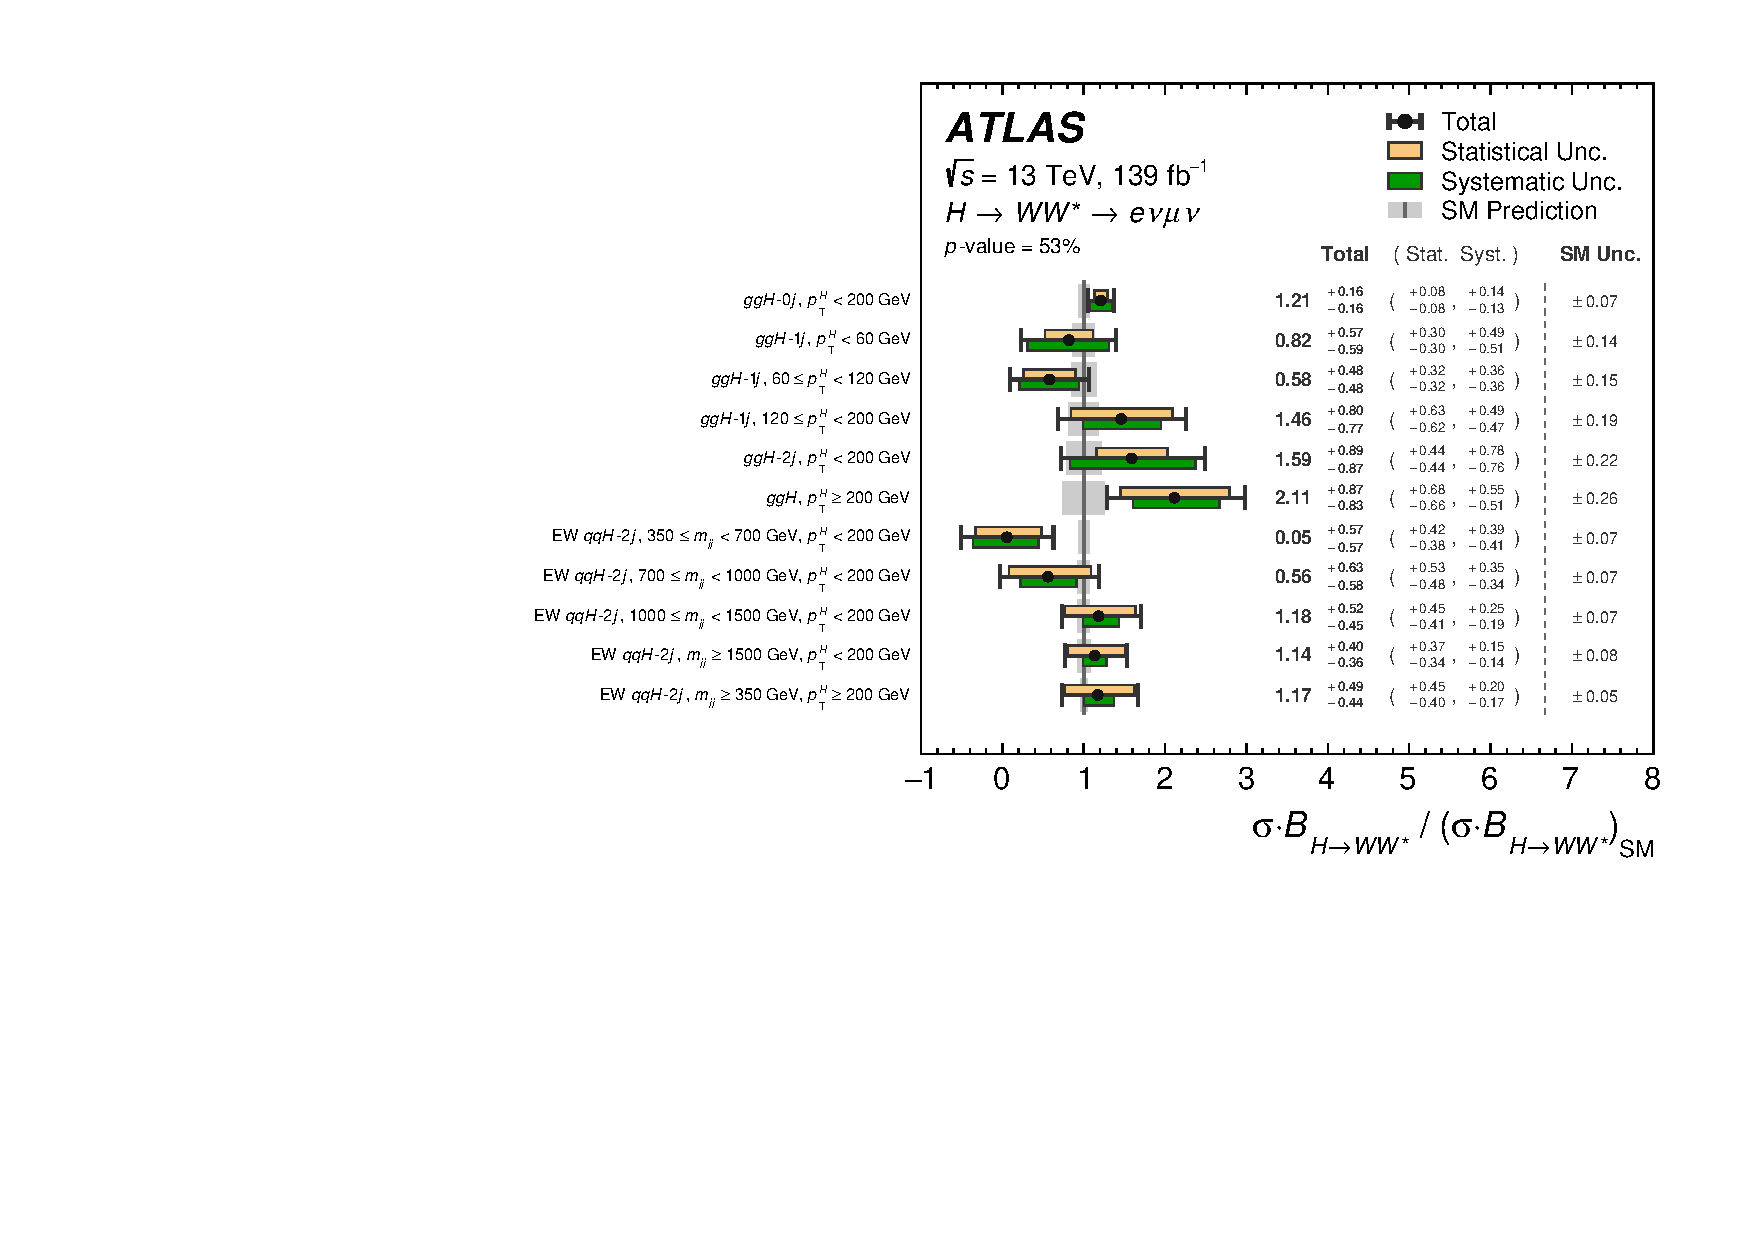
\includegraphics[width=0.9\textwidth]{\paperfiguredir/11-POI/plot-STXS-pois-GreenTan-vert.pdf}
  \caption{
    Best-fit value and uncertainties for the $\hww$ cross section measured in each of the STXS bins, normalized to the corresponding SM prediction.
    The black error bars, green boxes and tan boxes show the total, systematic, and statistical uncertainties in the measurements, respectively.
    The gray bands represent the theory uncertainty of the signal yield in the corresponding STXS bin.
    Figure and caption taken from \ccite{HWWPaper}.
    \label{fig:11-POI_measurement}
  }
\end{figure}

% STXS correlation matrix
%%%%%%%%%%%%%%%%%%%%%%%%%
\begin{figure}[htb]
  \centering
  \scalebox{0.8}{
    % \documentclass[tikz]{standalone}
% \usepackage{pgfplots}
% \begin{document}
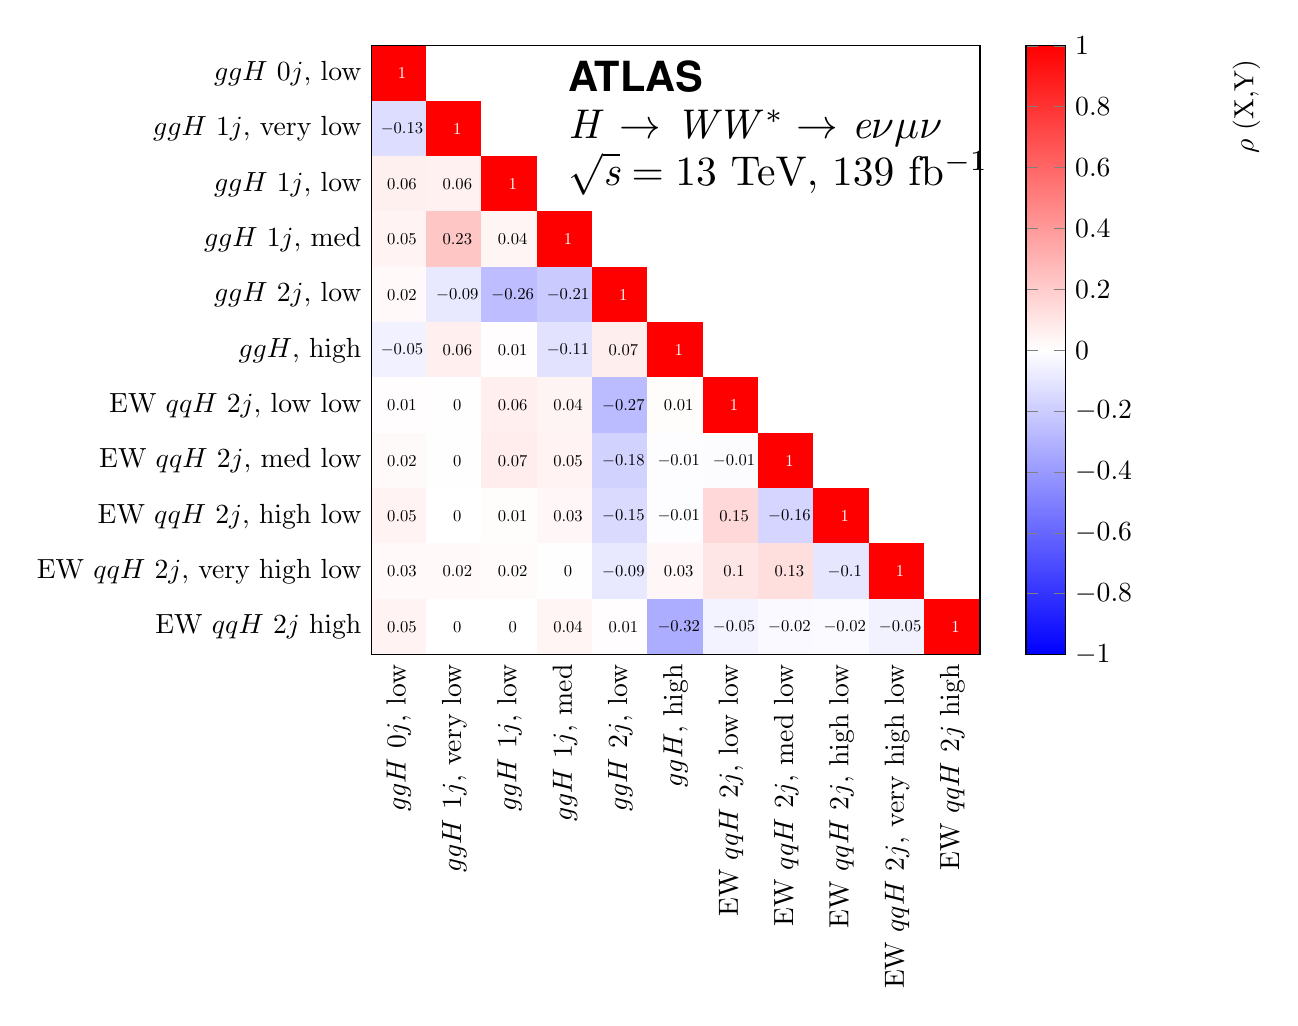
\begin{tikzpicture}
\begin{axis}[
    colormap={bluewhitered}{color=(blue) color=(white) color=(red)},
    clip=false,
    colorbar,
    colorbar style={
    ytick={-1,-0.8,...,1},
    ylabel={$\rho$ (X,Y)},
    ylabel style={
        at={(ticklabel cs:0.9)}
    },
    yticklabel style={
    text width=5em,
    ytick={-1,-0.8,...,1},
        tick style={draw=gray!}
        }
    },
    colormap name={bluewhitered},
   %  colormap/jet,
   % colorbar,
   % point meta min=0.0,
   % point meta max=0.2860,
   %  colorbar style={ height= 10 cm},xtick={0,0.286},
    % x=1em,
    % y=1em,
    x=2em,
    y=2em,
    xtick=data,
    ytick=data,
    ymin={$ggH~0j$, low \pTH},
    ymax={EW $qqH~2j$ high \pTH},
    xmin={$ggH~0j$, low \pTH},
    xmax={EW $qqH~2j$ high \pTH},
    y dir=reverse,
    % enlarge x limits={abs=0.5em},
    % enlarge y limits={abs=0.5em},
    enlarge x limits={abs=1em},
    enlarge y limits={abs=1em},
    point meta min=-1,
    point meta max=+1,
    % grid=both,
    major grid style={draw=none},
    visualization depends on={x\as\X},
    visualization depends on={y\as\Y},
    visualization depends on={correlations\as\Z},
    nodes near coords={\pgfmathtruncatemacro{\Z}
    {ifthenelse(\Y<\X,0,1)}
    \ifnum\Z=0
    \else\pgfmathprintnumber\pgfplotspointmeta\fi},
    % \ifthenelse{\X=+1}{\def\col{red}}{\def\col{black}},
    % every node near coord/.append style={anchor=center,scale=0.6,/pgf/number format/.cd,fixed,precision=2},
        % nodes near coord/.append={\pgfmathprintnumber\pgfplotspointmeta\,},
        % % ---------------------------------------------------------------------
        % % show `nodes near coords' but adapt the style so that values
        % % above a threshold get another style
        % % (adapted from <http://tex.stackexchange.com/a/141006/95441>)
        % % #1: the THRESHOLD after which we switch to a special display.
        nodes near coords black white/.style={
            small value/.style={
                text=black,
            },
            large value/.style={
                text=white,
            },
            every node near coord/.style={
                check for zero/.code={
                    \pgfmathfloatifflags{\pgfplotspointmeta}{0.0}{
                        % If meta=0, make the node a coordinate
                        % (which doesn't have text)
                        \pgfkeys{/tikz/coordinate}
                    }{
                        \begingroup
                        % this group is merely to switch to FPU locally.
                        % Might be unnecessary, but who knows.
                        \pgfkeys{/pgf/fpu}
                        \pgfmathparse{\pgfplotspointmeta<#1}
                        \global\let\result=\pgfmathresult
                        \endgroup
                        %
                        % simplifies debugging:
                        % \show\result
                        %
                        \pgfmathfloatcreate{0}{0.0}{0}
                        \let\ONE=\pgfmathresult
                        \ifx\result\ONE
                            \pgfkeysalso{/pgfplots/large value}
                        \else
                            \pgfkeysalso{/pgfplots/small value}
                        \fi
                    }
                },
                check for zero,
            }
        },
        % % asign a value to the new style thich is the threshold at which
        % % the two style `small value' or `large value' are used
        nodes near coords black white=0.9,
    every node near coord/.append style={font=\bfseries,anchor=center,scale=0.6,/pgf/number format/.cd,fixed,precision=2},
    minor tick num=1,
    symbolic x coords={{$ggH~0j$, low \pTH},{$ggH~1j$, very low \pTH},{$ggH~1j$, low \pTH},{$ggH~1j$, med \pTH},{$ggH~2j$, low \pTH},{$ggH$, high \pTH},{EW $qqH~2j$, low \mjj low \pTH},{EW $qqH~2j$, med \mjj low \pTH},{EW $qqH~2j$, high \mjj low \pTH},{EW $qqH~2j$, very high \mjj low \pTH},{EW $qqH~2j$ high \pTH}},
    symbolic y coords={{$ggH~0j$, low \pTH},{$ggH~1j$, very low \pTH},{$ggH~1j$, low \pTH},{$ggH~1j$, med \pTH},{$ggH~2j$, low \pTH},{$ggH$, high \pTH},{EW $qqH~2j$, low \mjj low \pTH},{EW $qqH~2j$, med \mjj low \pTH},{EW $qqH~2j$, high \mjj low \pTH},{EW $qqH~2j$, very high \mjj low \pTH},{EW $qqH~2j$ high \pTH}},
    axis on top,
    x tick label style={rotate=90},
    tick style={draw=none}
]
\addplot [matrix plot*,point meta=explicit,mesh/cols=11] table [meta=correlations] {
 x,  y,  correlations
 {$ggH~0j$, low \pTH} {$ggH~0j$, low \pTH} 1
 {$ggH~0j$, low \pTH} {$ggH~1j$, very low \pTH} -0.131324
 {$ggH~0j$, low \pTH} {$ggH~1j$, low \pTH}  0.059467
 {$ggH~0j$, low \pTH} {$ggH~1j$, med \pTH} 0.0490537
 {$ggH~0j$, low \pTH} {$ggH~2j$, low \pTH}  0.022738
 {$ggH~0j$, low \pTH} {$ggH$, high \pTH} -0.0546376
 {$ggH~0j$, low \pTH} {EW $qqH~2j$, low \mjj low \pTH} 0.0077486
 {$ggH~0j$, low \pTH} {EW $qqH~2j$, med \mjj low \pTH} 0.0211314
 {$ggH~0j$, low \pTH} {EW $qqH~2j$, high \mjj low \pTH}  0.0486984
 {$ggH~0j$, low \pTH} {EW $qqH~2j$, very high \mjj low \pTH} 0.0256006
 {$ggH~0j$, low \pTH} {EW $qqH~2j$ high \pTH} 0.0470472

 {$ggH~1j$, very low \pTH} {$ggH~0j$, low \pTH} 0
 {$ggH~1j$, very low \pTH} {$ggH~1j$, very low \pTH} 1
 {$ggH~1j$, very low \pTH} {$ggH~1j$, low \pTH}   0.0551626
 {$ggH~1j$, very low \pTH} {$ggH~1j$, med \pTH}  0.225791
 {$ggH~1j$, very low \pTH} {$ggH~2j$, low \pTH}   -0.0878372
 {$ggH~1j$, very low \pTH} {$ggH$, high \pTH}  0.0621163
 {$ggH~1j$, very low \pTH} {EW $qqH~2j$, low \mjj low \pTH}  0.00339789
 {$ggH~1j$, very low \pTH} {EW $qqH~2j$, med \mjj low \pTH}  0.0030145
 {$ggH~1j$, very low \pTH} {EW $qqH~2j$, high \mjj low \pTH}   0.00142807
 {$ggH~1j$, very low \pTH} {EW $qqH~2j$, very high \mjj low \pTH}   0.0224454
 {$ggH~1j$, very low \pTH} {EW $qqH~2j$ high \pTH} -0.00020307

 {$ggH~1j$, low \pTH}  {$ggH~0j$, low \pTH} 0
 {$ggH~1j$, low \pTH}  {$ggH~1j$, very low \pTH} 0
 {$ggH~1j$, low \pTH}  {$ggH~1j$, low \pTH}  1
 {$ggH~1j$, low \pTH}  {$ggH~1j$, med \pTH}  0.0382673
 {$ggH~1j$, low \pTH}  {$ggH~2j$, low \pTH}   -0.260164
 {$ggH~1j$, low \pTH}  {$ggH$, high \pTH}  0.00778543
 {$ggH~1j$, low \pTH}  {EW $qqH~2j$, low \mjj low \pTH}  0.0640812
 {$ggH~1j$, low \pTH}  {EW $qqH~2j$, med \mjj low \pTH}  0.0702857
 {$ggH~1j$, low \pTH}  {EW $qqH~2j$, high \mjj low \pTH}   0.014091
 {$ggH~1j$, low \pTH}  {EW $qqH~2j$, very high \mjj low \pTH}  0.0167539
 {$ggH~1j$, low \pTH}  {EW $qqH~2j$ high \pTH}  0.00113077

 {$ggH~1j$, med \pTH} {$ggH~0j$, low \pTH} 0
 {$ggH~1j$, med \pTH} {$ggH~1j$, very low \pTH} 0
 {$ggH~1j$, med \pTH} {$ggH~1j$, low \pTH}  0
 {$ggH~1j$, med \pTH} {$ggH~1j$, med \pTH} 1
 {$ggH~1j$, med \pTH} {$ggH~2j$, low \pTH}  -0.207511
 {$ggH~1j$, med \pTH} {$ggH$, high \pTH} -0.114735
 {$ggH~1j$, med \pTH} {EW $qqH~2j$, low \mjj low \pTH} 0.0425279
 {$ggH~1j$, med \pTH} {EW $qqH~2j$, med \mjj low \pTH} 0.0476515
 {$ggH~1j$, med \pTH} {EW $qqH~2j$, high \mjj low \pTH}  0.0336961
 {$ggH~1j$, med \pTH} {EW $qqH~2j$, very high \mjj low \pTH} 0.00431544
 {$ggH~1j$, med \pTH} {EW $qqH~2j$ high \pTH} 0.0390297

 {$ggH~2j$, low \pTH}  {$ggH~0j$, low \pTH} 0
 {$ggH~2j$, low \pTH}  {$ggH~1j$, very low \pTH} 0
 {$ggH~2j$, low \pTH}  {$ggH~1j$, low \pTH}  0
 {$ggH~2j$, low \pTH}  {$ggH~1j$, med \pTH} 0
 {$ggH~2j$, low \pTH}  {$ggH~2j$, low \pTH}  1
 {$ggH~2j$, low \pTH}  {$ggH$, high \pTH} 0.0669787
 {$ggH~2j$, low \pTH}  {EW $qqH~2j$, low \mjj low \pTH} -0.265444
 {$ggH~2j$, low \pTH}  {EW $qqH~2j$, med \mjj low \pTH} -0.176917
 {$ggH~2j$, low \pTH}  {EW $qqH~2j$, high \mjj low \pTH}  -0.145543
 {$ggH~2j$, low \pTH}  {EW $qqH~2j$, very high \mjj low \pTH} -0.0889487
 {$ggH~2j$, low \pTH}  {EW $qqH~2j$ high \pTH} 0.00671903

 {$ggH$, high \pTH} {$ggH~0j$, low \pTH} 0
 {$ggH$, high \pTH} {$ggH~1j$, very low \pTH} 0
 {$ggH$, high \pTH} {$ggH~1j$, low \pTH}  0
 {$ggH$, high \pTH} {$ggH~1j$, med \pTH} 0
 {$ggH$, high \pTH} {$ggH~2j$, low \pTH}  0
 {$ggH$, high \pTH} {$ggH$, high \pTH} 1
 {$ggH$, high \pTH} {EW $qqH~2j$, low \mjj low \pTH} 0.0119376
 {$ggH$, high \pTH} {EW $qqH~2j$, med \mjj low \pTH} -0.00631914
 {$ggH$, high \pTH} {EW $qqH~2j$, high \mjj low \pTH}  -0.0071606
 {$ggH$, high \pTH} {EW $qqH~2j$, very high \mjj low \pTH} 0.0303077
 {$ggH$, high \pTH} {EW $qqH~2j$ high \pTH} -0.322628

 {EW $qqH~2j$, low \mjj low \pTH} {$ggH~0j$, low \pTH} 0
 {EW $qqH~2j$, low \mjj low \pTH} {$ggH~1j$, very low \pTH} 0
 {EW $qqH~2j$, low \mjj low \pTH} {$ggH~1j$, low \pTH} 0
 {EW $qqH~2j$, low \mjj low \pTH} {$ggH~1j$, med \pTH} 0
 {EW $qqH~2j$, low \mjj low \pTH} {$ggH~2j$, low \pTH} 0
 {EW $qqH~2j$, low \mjj low \pTH} {$ggH$, high \pTH} 0
 {EW $qqH~2j$, low \mjj low \pTH} {EW $qqH~2j$, low \mjj low \pTH} 1
 {EW $qqH~2j$, low \mjj low \pTH} {EW $qqH~2j$, med \mjj low \pTH} -0.0093563
 {EW $qqH~2j$, low \mjj low \pTH} {EW $qqH~2j$, high \mjj low \pTH}  0.148795
 {EW $qqH~2j$, low \mjj low \pTH} {EW $qqH~2j$, very high \mjj low \pTH} 0.0993198
 {EW $qqH~2j$, low \mjj low \pTH} {EW $qqH~2j$ high \pTH} -0.0476769

 {EW $qqH~2j$, med \mjj low \pTH} {$ggH~0j$, low \pTH} 0
 {EW $qqH~2j$, med \mjj low \pTH} {$ggH~1j$, very low \pTH} 0
 {EW $qqH~2j$, med \mjj low \pTH} {$ggH~1j$, low \pTH} 0
 {EW $qqH~2j$, med \mjj low \pTH} {$ggH~1j$, med \pTH} 0
 {EW $qqH~2j$, med \mjj low \pTH} {$ggH~2j$, low \pTH} 0
 {EW $qqH~2j$, med \mjj low \pTH} {$ggH$, high \pTH} 0
 {EW $qqH~2j$, med \mjj low \pTH} {EW $qqH~2j$, low \mjj low \pTH} 0
 {EW $qqH~2j$, med \mjj low \pTH} {EW $qqH~2j$, med \mjj low \pTH} 1
 {EW $qqH~2j$, med \mjj low \pTH} {EW $qqH~2j$, high \mjj low \pTH}  -0.162325
 {EW $qqH~2j$, med \mjj low \pTH} {EW $qqH~2j$, very high \mjj low \pTH} 0.129734
 {EW $qqH~2j$, med \mjj low \pTH} {EW $qqH~2j$ high \pTH} -0.0214162


 {EW $qqH~2j$, high \mjj low \pTH}  {$ggH~0j$, low \pTH} 0
 {EW $qqH~2j$, high \mjj low \pTH}  {$ggH~1j$, very low \pTH} 0
 {EW $qqH~2j$, high \mjj low \pTH}  {$ggH~1j$, low \pTH} 0
 {EW $qqH~2j$, high \mjj low \pTH}  {$ggH~1j$, med \pTH} 0
 {EW $qqH~2j$, high \mjj low \pTH}  {$ggH~2j$, low \pTH} 0
 {EW $qqH~2j$, high \mjj low \pTH}  {$ggH$, high \pTH} 0
 {EW $qqH~2j$, high \mjj low \pTH}  {EW $qqH~2j$, low \mjj low \pTH} 0
 {EW $qqH~2j$, high \mjj low \pTH}  {EW $qqH~2j$, med \mjj low \pTH} 0
 {EW $qqH~2j$, high \mjj low \pTH}  {EW $qqH~2j$, high \mjj low \pTH}  1
 {EW $qqH~2j$, high \mjj low \pTH}  {EW $qqH~2j$, very high \mjj low \pTH} -0.0961078
 {EW $qqH~2j$, high \mjj low \pTH}  {EW $qqH~2j$ high \pTH} -0.0200312

 {EW $qqH~2j$, very high \mjj low \pTH} {$ggH~0j$, low \pTH} 0
 {EW $qqH~2j$, very high \mjj low \pTH} {$ggH~1j$, very low \pTH} 0
 {EW $qqH~2j$, very high \mjj low \pTH} {$ggH~1j$, low \pTH} 0
 {EW $qqH~2j$, very high \mjj low \pTH} {$ggH~1j$, med \pTH} 0
 {EW $qqH~2j$, very high \mjj low \pTH} {$ggH~2j$, low \pTH} 0
 {EW $qqH~2j$, very high \mjj low \pTH} {$ggH$, high \pTH} 0
 {EW $qqH~2j$, very high \mjj low \pTH} {EW $qqH~2j$, low \mjj low \pTH} 0
 {EW $qqH~2j$, very high \mjj low \pTH} {EW $qqH~2j$, med \mjj low \pTH} 0
 {EW $qqH~2j$, very high \mjj low \pTH} {EW $qqH~2j$, high \mjj low \pTH} 0
 {EW $qqH~2j$, very high \mjj low \pTH} {EW $qqH~2j$, very high \mjj low \pTH} 1
 {EW $qqH~2j$, very high \mjj low \pTH} {EW $qqH~2j$ high \pTH} -0.0513732

 {EW $qqH~2j$ high \pTH} {$ggH~0j$, low \pTH} 0
 {EW $qqH~2j$ high \pTH} {$ggH~1j$, very low \pTH} 0
 {EW $qqH~2j$ high \pTH} {$ggH~1j$, low \pTH} 0
 {EW $qqH~2j$ high \pTH} {$ggH~1j$, med \pTH} 0
 {EW $qqH~2j$ high \pTH} {$ggH~2j$, low \pTH} 0
 {EW $qqH~2j$ high \pTH} {$ggH$, high \pTH} 0
 {EW $qqH~2j$ high \pTH} {EW $qqH~2j$, low \mjj low \pTH} 0
 {EW $qqH~2j$ high \pTH} {EW $qqH~2j$, med \mjj low \pTH} 0
 {EW $qqH~2j$ high \pTH} {EW $qqH~2j$, high \mjj low \pTH} 0
 {EW $qqH~2j$ high \pTH} {EW $qqH~2j$, very high \mjj low \pTH} 0
 {EW $qqH~2j$ high \pTH} {EW $qqH~2j$ high \pTH} 1
};
\node (atlas) [above right, font={\fontfamily{phv}\fontseries{b}\selectfont},scale=1.5] at (rel axis cs:0.3,0.9) {ATLAS};
% \node (internal) [anchor=west,scale=1.5] at (atlas.east) {Internal};
\node (secondline)[above right,scale=1.5] at (rel axis cs:0.3,0.81) {\emph{H} $\to$ \emph{WW}$^{*} \to$ \emph{e$\nu\mu\nu$}};
\node (thirdline)[above right,scale=1.5] at (rel axis cs:0.3,0.73) {$\sqrt{\emph{s}} = 13$ TeV, 139 fb$^{-1}$};
%\node[rotate=90] at (120,100){$\rho$ (X,Y)};
\end{axis}
\end{tikzpicture}
% \end{document}

    %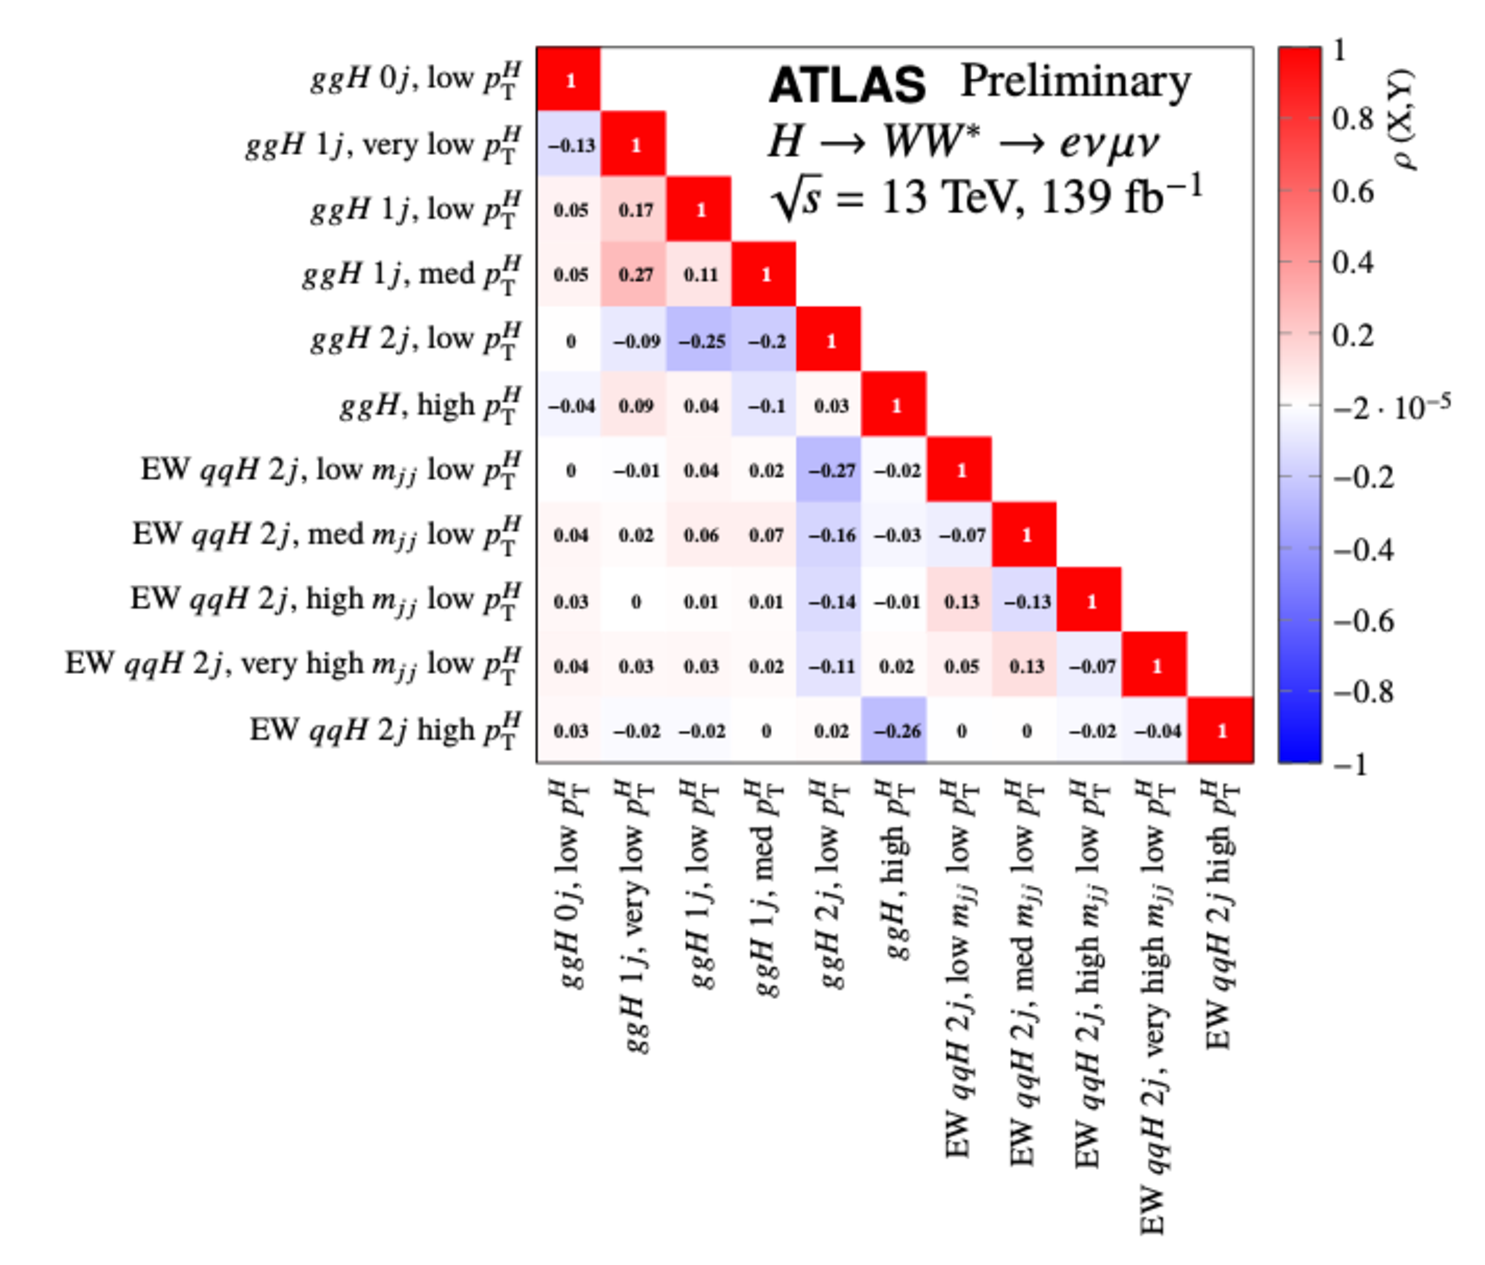
\includegraphics[width=1.2\textwidth]{\paperfiguredir/CorrelationMatrix} % Only to be used for the figure extraction script
  }
  \caption{
    Correlations between the cross-section measurements in the 11 STXS bins for the \hwwenmn analysis.
    Figure and caption taken from \ccite{HWWPaper}.
    \label{fig:STXS-correlation}
  }
\end{figure}

\subsection{Post-fit distributions and signal excess}
Post-fit distributions are presented that show the expected yields when all parameters are set to their corresponding post-fit values. They also take properly into account all systematic uncertainties. \Cref{fig:VBF_DNN} shows the post-fit DNN output distribution in the VBF SR as obtained from the 2-PoI fit.
The VBF signal can be well separated from the backgrounds up to a signal-to-background ratio of more than two in the highest DNN bin. 
The VBF signal is observed with a discovery significance of $5.8\,\sigma$, where $6.2\,\sigma$ were expected.
% The observed (expected) VBF signal reaches a significance of $5.8\sigma$ ($6.2\sigma$) above the background expectation.
The post-fit \mT distributions in the different ggF SRs as well as in the combined region are shown in \cref{fig:ggF_MT}.
The ggF events with two jets in the final state are measured with a discovery significance of $2.2\sigma$, where $1.6\sigma$ were expected. In this fit, the VBF contribution is fixed to the SM prediction.

Representative post-fit distributions for the STXS measurements are shown in \cref{fig:aux:VBF-STXS-SRs}, corresponding to VBF STXS SRs targeting EW~$qqH$ production. 
Especially in the high \mjj bins, the measured VBF signal is very prominent above the backgrounds. 

For all distributions shown, the observed yields agree in both shapes and rates with the SM expectations.
Similarly, post-fit distributions of other observables were studied and are found in excellent agreement with their expectations. The post-fit distributions of the final discriminants in the CRs are provided in \cref{app:post-fit-distributions}. 

\begin{figure}[htb]
  \centering
  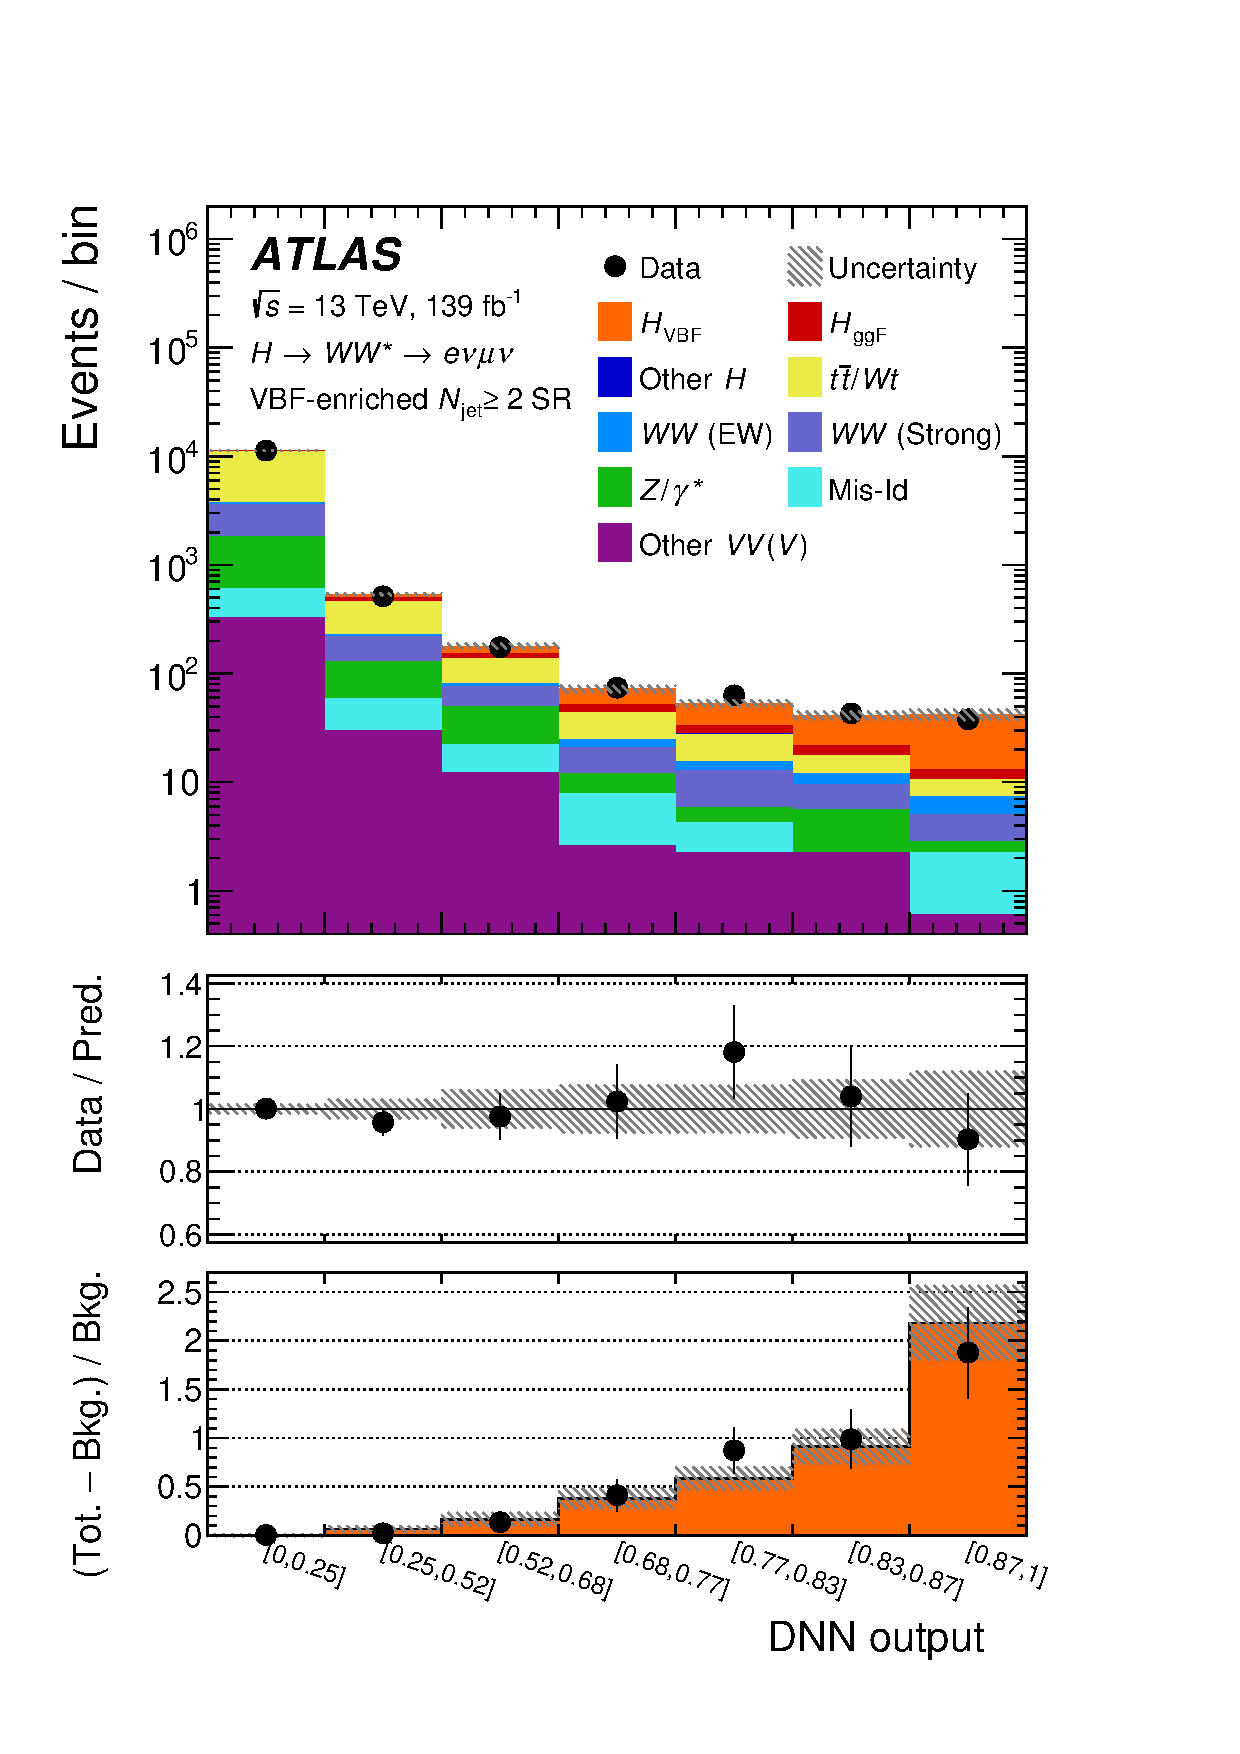
\includegraphics[width=0.65\textwidth]{\paperfiguredir/VBF/SR/PostFit_VBF_DNN_ratios_SR_HWWRun2VBF_HWWVBF.pdf}
  \caption{
    Post-fit distribution of the DNN output in the VBF signal region.
    The hatched band shows the total uncertainty, assuming SM Higgs boson production.
    The middle panel shows the ratio of the data to the sum of the fitted signal and background.
    The bottom panel displays the signal-to-background ratio, where the hatched band indicates the combined statistical and systematic uncertainty for the fitted signal and background.
    Figure and caption taken from \ccite{HWWPaper}
  }
  \label{fig:VBF_DNN}
\end{figure}

\begin{figure}[htb]
  \centering
  \subfloat[]{
    \includegraphics[width=0.355\textwidth]{\paperfiguredir/ggF/ZeroJet/moneyplot-0j}
  }
  \subfloat[]{
    \includegraphics[width=0.355\textwidth]{\paperfiguredir/ggF/OneJet/moneyplot-1j}
  } \\
  \subfloat[]{
    \includegraphics[width=0.355\textwidth]{\paperfiguredir/ggF/TwoJet/moneyplot-2j}
  }
  \subfloat[]{
    \includegraphics[width=0.355\textwidth]{\paperfiguredir/ggF/Combined/moneyplot-combined}
  }
  \caption{
    Post-fit $\mT$ distributions with the signal and the background modeled contributions
    in the (a) $\ZeroJet$, (b) $\OneJet$, (c) ggF-enriched \TwoJet, and (d) combined ggF signal regions. Underflow and overflow events are not included.
    The hatched band shows the total uncertainty, assuming SM Higgs boson production.
    The middle panel shows the ratio of the data to the sum of the fitted signal and background.
    The bottom panel displays the difference between the data and the estimated background compared to the simulated signal distribution, where the hatched band indicates the combined statistical and systematic uncertainty for the fitted signal and background.
    Figure and caption taken from \cref{HWWPaper}. 
    \label{fig:ggF_MT}
  }
\end{figure}

% DNN distribution in 5 VBF STXS SRs
\begin{figure}[!h]
  \centering
  \subfloat[]{
    \includegraphics[width=0.32\textwidth]{\paperfiguredir/VBFSTXS/PostFit_VBF_DNN_SR_VBF2J_MJJ_350_700_PTH_0_200_HWWVBF}
  }
  \subfloat[]{
    \includegraphics[width=0.32\textwidth]{\paperfiguredir/VBFSTXS/PostFit_VBF_DNN_SR_VBF2J_MJJ_700_1000_PTH_0_200_HWWVBF}
  }
  \subfloat[]{
    \includegraphics[width=0.32\textwidth]{\paperfiguredir/VBFSTXS/PostFit_VBF_DNN_SR_VBF2J_MJJ_1000_1500_PTH_0_200_HWWVBF}
  } \\
  \subfloat[]{
    \includegraphics[width=0.32\textwidth]{\paperfiguredir/VBFSTXS/PostFit_VBF_DNN_SR_VBF2J_MJJ_GT1500_PTH_0_200_HWWVBF}
  }
  \subfloat[]{
    \includegraphics[width=0.32\textwidth]{\paperfiguredir/VBFSTXS/PostFit_VBF_DNN_SR_VBF2J_PTH_GT200_HWWVBF}
  }
  \caption{
    Post-fit DNN output distributions in the VBF STXS signal regions with the binning used in the STXS fit.
    The hatched bands indicate the combined statistical and systematic uncertainty for the fitted signal and background.
    The signal process targeted by the respective signal region is labelled as $H_{\text{EW } qqH}^{\mathrm{target}}$, the other signal processes are summed and collectively denoted $H_{\text{EW } qqH}$. 
    Figure and caption taken from \cref{HWWPaper}. 
    \label{fig:aux:VBF-STXS-SRs}
  }
\end{figure}

% Table with yields in each STXS SR (likely to go in auxiliary material)
%%%%%%%%%%%%%%%%%%%%%%%%%%%%%%%%%%%%####################################
% Table with STXS XSec measurements and their uncertainties
%%%%%%%%%%%%%%%%%%%%%%%%%%%%%%%%%%%%%%%%%%%%%%%%%%%%%%%%%%%%%%%%%%%%%%%%%%%%%

% From paper:
% The measurements are dominated by systematic uncertainties.
% For the ggF measurement, uncertainties from experimental and theoretical sources are comparable.
% For the VBF measurement, signal theory uncertainties make up the largest contribution and the dominant ones are those related to the modeling of potential jets in addition to the tagging jets.



\FloatBarrier
\section{Discussion and Possible Improvements}
\label{sec:hww:summary}
\documentclass{article}
\usepackage[a4paper,margin=2cm]{geometry}
\title{Analysis Summary}
\author{generated with CAFCore/CommonAnalysisHelpers by user bjager}
\date{08-06-2022}
\usepackage{adjustbox}
\usepackage{graphicx}
\usepackage[subpreambles]{standalone}
\usepackage{fancyhdr}
\pagestyle{fancy}
\setcounter{secnumdepth}{0}
\usepackage{tikz}
\usetikzlibrary{positioning,arrows}
\usepackage{hyperref}
\usepackage[open]{bookmark}
\begin{document}
\maketitle
\tableofcontents

\begin{itemize}
\item \textbf{prepare} was run on \textbf{Tue Sep 28 09:53:31 2021} compiled with gcc 8.3.0 under ROOT 6.18/04 using the configuration \textbf{'config/master/VBF/prepare-VBF-default.cfg'} with options \textbf{'outputFile=sampleFolders/prepared/210924-samples-prepared.root'} \item \textbf{initialize} was run on \textbf{Tue Sep 28 11:15:28 2021} compiled with gcc 8.3.0 under ROOT 6.18/04 using the configuration \textbf{'config/master/VBF/initialize-VBF-default.cfg'} with options \textbf{'outputFile=/project/ctb-stelzer/bjager/CAFoutput/batchOutput/unmerged\_210928-initialized-nom/unmerged\_210928-initialized-nom\_sig\_X\_c16e\_vh.root', 'inputFile=sampleFolders/prepared/210924-samples-prepared.root', 'campaignsConfig=config/master/common/campaigns-cedar-V21-PFlowJets-skimmed.cfg', 'prettyPrint=false', 'lineUpdates=false', 'prettyPrint=false', 'lineUpdates=false', 'prettyPrint=false', 'lineUpdates=false', 'prettyPrint=false', 'lineUpdates=false', 'prettyPrint=false', 'lineUpdates=false', 'prettyPrint=false', 'lineUpdates=false', 'prettyPrint=false', 'lineUpdates=false', 'prettyPrint=false', 'lineUpdates=false', 'prettyPrint=false', 'lineUpdates=false', 'prettyPrint=false', 'lineUpdates=false', 'prettyPrint=false', 'lineUpdates=false', 'prettyPrint=false', 'lineUpdates=false', 'prettyPrint=false', 'lineUpdates=false', 'prettyPrint=false', 'lineUpdates=false', 'prettyPrint=false', 'lineUpdates=false', 'prettyPrint=false', 'lineUpdates=false', 'prettyPrint=false', 'lineUpdates=false', 'prettyPrint=false', 'lineUpdates=false', 'prettyPrint=false', 'lineUpdates=false', 'prettyPrint=false', 'lineUpdates=false', 'prettyPrint=false', 'lineUpdates=false', 'prettyPrint=false', 'lineUpdates=false', 'prettyPrint=false', 'lineUpdates=false', 'prettyPrint=false', 'lineUpdates=false', 'prettyPrint=false', 'lineUpdates=false', 'prettyPrint=false', 'lineUpdates=false', 'prettyPrint=false', 'lineUpdates=false', 'prettyPrint=false', 'lineUpdates=false', 'prettyPrint=false', 'lineUpdates=false', 'prettyPrint=false', 'lineUpdates=false', 'prettyPrint=false', 'lineUpdates=false', 'prettyPrint=false', 'lineUpdates=false', 'prettyPrint=false', 'lineUpdates=false', 'prettyPrint=false', 'lineUpdates=false', 'prettyPrint=false', 'lineUpdates=false', 'prettyPrint=false', 'lineUpdates=false', 'prettyPrint=false', 'lineUpdates=false', 'prettyPrint=false', 'lineUpdates=false', 'prettyPrint=false', 'lineUpdates=false', 'prettyPrint=false', 'lineUpdates=false', 'prettyPrint=false', 'lineUpdates=false', 'prettyPrint=false', 'lineUpdates=false', 'prettyPrint=false', 'lineUpdates=false', 'prettyPrint=false', 'lineUpdates=false', 'prettyPrint=false', 'lineUpdates=false', 'prettyPrint=false', 'lineUpdates=false', 'inputFile=sampleFolders/prepared/210924-samples-prepared.root', 'campaignsConfig=config/master/common/campaigns-cedar-V21-PFlowJets-skimmed.cfg'} \item \textbf{analyze} was run on \textbf{Wed Sep 29 17:55:57 2021} compiled with gcc 8.3.0 under ROOT 6.18/04 using the configuration \textbf{'config/master/STXS/analyze-VBF-STXS-nominal.cfg'} with options \textbf{'outputFile=/project/ctb-stelzer/bjager/CAFoutput/batchOutput/unmerged\_210924-VBF-nom-4/unmerged\_210924-VBF-nom-4\_sig\_X\_X\_vh.part6.root', 'inputFile=sampleFolders/initialized/210928-samples-initialized-nom.root', 'prettyPrint=false', 'lineUpdates=false', 'prettyPrint=false', 'lineUpdates=false', 'prettyPrint=false', 'lineUpdates=false', 'prettyPrint=false', 'lineUpdates=false', 'prettyPrint=false', 'lineUpdates=false', 'inputFile=sampleFolders/initialized/210928-samples-initialized-nom.root'} \item \textbf{visualize} was run on \textbf{Wed Jun  8 23:19:24 2022} compiled with gcc 8.3.0 under ROOT 6.18/04 using the configuration \textbf{'config/master/VBF/visualize-VBF-default.cfg'} with options \textbf{'inputFile=/project/ctb-stelzer/bjager/CAFoutput/FullRun2PaperWorkspaces/210924-4-samples-analyzed-VBF-nom.root', 'outputDir=results/220605-Thesis/sr/mt', 'doNFs=false', 'makePlots=CutVBF\_SR/MT,CutVBF\_SR/MT\_2,CutVBF\_WWControl\_2jet/MT\_4', 'makeLogPlots=true', 'histogramProcesses=config/visualization/processes/VBF/prefit-nfs-sr.txt', 'patches=config/visualization/style/VBF/VBF-style-post-fit-noLines.txt', 'plotter.geometry.legend.xMin=0.50', 'plotter.geometry.legend.yMin=0.7', 'plotter.geometry.legend.xMax=0.92', 'plotter.geometry.legend.yMax=0.92', 'plotter.legend.showTotalBkgErrorType=false', 'plotter.legend.showTotalBkgErrorType=false', 'plotter.style.legend.showTotalBkgErrorType=false', 'geometry.main.yAxis.titleOffset=1.2', 'plotter.style.legend.errorDisplayType=f', 'plotter.style.listSignalFirst=true', 'plotter.style.stackSignal=true', 'plotter.style.manualStacking=true', 'plotter.style.reverseStacking=true', 'plotter.style.unsorted=true', 'plotter.style.listDataFirst=true', 'plotter.style.nLegendCols=2', 'plotter.style.sub.yAxis.nDiv=505', 'plotter.style.main.totalStackError.fillStyle=3245', 'plotter.style.ratioMax=1.45', 'plotter.style.ratioMin=0.55', 'plotter.style.legend.textSize=0.03', 'plotter.style.min=0', 'plotter.style.autoStackLegend=true', 'plotter.style.autoStackSignal=true', 'plotter.labels.legendTotalBkg=Uncertainty', 'plotter.labels.drawInfo=false', 'plotter.style.main.totalStack.lineWidth=0', 'plotter.style.main.totalStack.lineColor=kWhite', 'plotter.style.sub.margin=1.2', 'plotter.style.labels.yPos=0.93', 'plotter.style.labels.xOffset=0.19', 'plotter.legend.dataDisplayType=lep', 'plotter.style.forceRatioLimits=true', 'plotter.style.showOverflow=true', 'plotter.labels.totalStack=Pred.', 'plotter.labels.drawATLAS=false', 'labels.drawATLAS=false', 'plotter.style.labels.drawATLAS=false', 'plotter.style.showRatio=true', 'plotter.style.max.scale=0.9', 'makeCutflows=false', 'systematicsBands=auxData/systematicsBands/VBF/210927-systematics-reduced-band-file.root:systematics>>::emme', 'plotter.errors.showSys=emme', 'plotter.errors.source=totalStack', 'plotter.errors.shiftTo=totalStack', 'plotter.errors.normSys=true', 'plotter.errors.shapeSys=false', 'plotter.verbose=false', 'plotter.labels.axes.mainY=Events / 30 GeV', 'plotter.labels.axes.subX=m\_{T} GeV'} \end{itemize}
\section[Cut Overview]{Cut Overview}

\centering

\adjustbox{width=\textwidth,height=\textheight,keepaspectratio}{\documentclass{standalone}
\usepackage{tikz}
\usepackage{underscore}
\usepackage[T1]{fontenc}
\usetikzlibrary{positioning,arrows}
\begin{document}
\begingroup
\tikzstyle{block} = [rectangle, draw, fill=blue!20, text width=10em, inner sep=2.5pt, text centered, rounded corners, minimum height=2em]
\tikzstyle{job} = [rectangle, draw, fill=red!20, inner sep=2.5pt, rounded corners, font={\tiny}]
\tikzstyle{line} = [draw, -latex']

\begin{tikzpicture}[]
\node [block] (basecut) {__baseCut__};
\node [block, below=of basecut] (cutstxs) {Signal split into STXS bins};
\node [block, below=of cutstxs] (cutchannels) {Channel Selection};
\node [block, below=of cutchannels] (cuttrigger) {Trigger Selection};
\node [block, below=of cuttrigger] (cuttriggermatch) {Trigger Matching};
\node [block, below=of cuttriggermatch] (cutdatadrivenmufake) {W+jets flavour split muon};
\node [block, below=of cutdatadrivenmufake] (cutdatadrivenelfake) {W+jets flavour split electron};
\node [block, below=of cutdatadrivenelfake] (cutjetcleaning) {Jet Cleaning};
\node [block, below=of cutjetcleaning] (cutvgammavjetoverlap) {Overlap: Vgamma/Vjets};
\node [block, below=of cutvgammavjetoverlap] (cut2leptons) {Only two Leptons};
\node [block, below=of cut2leptons] (cutleadleptonpt) {$p_{t}^{lead} > 22$ GeV};
\node [block, below=of cutleadleptonpt] (cutsubleadleptonpt) {$p_{t}^{\rm sublead} > 15$};
\node [block, below=of cutsubleadleptonpt] (cutremovehigheventweights) {Remove High Eventweight Events};
\node [block, below=of cutremovehigheventweights] (cutosleptons) {OS Leptons};
\node [block, below=of cutosleptons] (cutmll) {$M_{\ell\ell} > 12/10$ GeV};
\node [block, below=of cutmll] (cutzveto) {SF: Z Veto};
\node [block, below=of cutzveto] (cutlepselection) {Leptons ID, singleFakes 1 anti-ID,1 ID, doubleFakes 2*anti-ID};
\node [block, below=of cutlepselection] (cutqcdff) {Apply QCD FF weight};
\node [block, below=of cutqcdff] (cutff) {Apply fake factor};
\node [block, below=of cutff] (cutvbf2jet) {2-jet (30,30) fJVT};
\node [block, below=of cutvbf2jet] (cutvbfbveto2jet) {b-veto};
\node [block, below=of cutvbfbveto2jet] (cutvbfztautaucontrolbveto2jet) {$Z\to\tau\tau$ CR: $\vert m_{\tau\tau}-m_Z\vert<$ 25, bVeto};
\node [block, below=of cutvbfztautaucontrolbveto2jet] (cutvbfztautaucontrolbveto2jetmllmet) {$Z\to\tau\tau$ CR: $M_{ll}<70$ GeV};
\node [block, below=of cutvbfztautaucontrolbveto2jetmllmet] (cutvbfztautaucontrol2jetinclcjv) {$Z\to\tau\tau$ CR: CJV$<30$ GeV};
\node [block, below=of cutvbfztautaucontrol2jetinclcjv] (cutvbfztautaucontrol2jetinclolv) {$Z\to\tau\tau$ CR: OLV};
\node [block, below=of cutvbfztautaucontrol2jetinclolv] (cutvbfztautaucontrol2jet) {Ztautau CR};
\node [block, below=of cutvbfztautaucontrol2jet] (cutvbfztautaucontrol2jetmjjgt350) {qq2Hqq_MJJ_GT350};
\node [block, below=of cutvbfztautaucontrol2jetmjjgt350] (cutvbfztautaucontrol2jetmjjgt350pth0200) {ZttCR_qq2Hqq_2J_PTH_0_200};
\node [block, below=of cutvbfztautaucontrol2jetmjjgt350pth0200] (cutvbfztautaucontrol2jetmjjgt700pth0200) {ZttCR_qq2Hqq_2J_MJJ_GT700_PTH_0_200};
\node [block, below=of cutvbfztautaucontrol2jetmjjgt700pth0200] (cutvbfztautaucontrol2jetmjj10001500pth0200) {ZttCR_qq2Hqq_2J_MJJ_1000_1500_PTH_0_200};
\node [block, below=of cutvbfztautaucontrol2jetmjj10001500pth0200] (cutvbfztautaucontrol2jetmjj10001500pth0200pthjj025) {ZttCR_qq2Hqq_2J_MJJ_1000_1500_PTH_0_200_PTHJJ_0_25};
\path [line] (node cs:name=cutvbfztautaucontrol2jetmjj10001500pth0200, anchor=south) -| (node cs:name=cutvbfztautaucontrol2jetmjj10001500pth0200pthjj025, anchor=north);
\node [block, right=1*0.1cm+0*(10em+2*2.5pt) of cutvbfztautaucontrol2jetmjj10001500pth0200pthjj025] (cutvbfztautaucontrol2jetmjj10001500pth0200pthjjgt25) {ZttCR_qq2Hqq_2J_MJJ_1000_1500_PTH_0_200_PTHJJ_GT25};
\path [line] (node cs:name=cutvbfztautaucontrol2jetmjj10001500pth0200, anchor=east) -| (node cs:name=cutvbfztautaucontrol2jetmjj10001500pth0200pthjjgt25, anchor=north);
\path [line] (node cs:name=cutvbfztautaucontrol2jetmjjgt700pth0200, anchor=south) -| (node cs:name=cutvbfztautaucontrol2jetmjj10001500pth0200, anchor=north);
\node [block, right=2*0.1cm+1*(10em+2*2.5pt) of cutvbfztautaucontrol2jetmjj10001500pth0200] (cutvbfztautaucontrol2jetmjjgt1500pth0200) {ZttCR_qq2Hqq_2J_MJJ_GT1500_PTH_0_200};
\node [block, below=of cutvbfztautaucontrol2jetmjjgt1500pth0200] (cutvbfztautaucontrol2jetmjjgt1500pth0200pthjj025) {ZttCR_qq2Hqq_2J_MJJ_GT1500_PTH_0_200_PTHJJ_0_25};
\path [line] (node cs:name=cutvbfztautaucontrol2jetmjjgt1500pth0200, anchor=south) -| (node cs:name=cutvbfztautaucontrol2jetmjjgt1500pth0200pthjj025, anchor=north);
\node [block, right=1*0.1cm+0*(10em+2*2.5pt) of cutvbfztautaucontrol2jetmjjgt1500pth0200pthjj025] (cutvbfztautaucontrol2jetmjjgt1500pth0200pthjjgt25) {ZttCR_qq2Hqq_2J_MJJ_GT1500_PTH_0_200_PTHJJ_GT25};
\path [line] (node cs:name=cutvbfztautaucontrol2jetmjjgt1500pth0200, anchor=east) -| (node cs:name=cutvbfztautaucontrol2jetmjjgt1500pth0200pthjjgt25, anchor=north);
\path [line] (node cs:name=cutvbfztautaucontrol2jetmjjgt700pth0200, anchor=east) -| (node cs:name=cutvbfztautaucontrol2jetmjjgt1500pth0200, anchor=north);
\node [block, right=2*0.1cm+1*(10em+2*2.5pt) of cutvbfztautaucontrol2jetmjjgt1500pth0200] (cutvbfztautaucontrol2jetmjj7001000pth0200) {ZttCR_qq2Hqq_2J_MJJ_700_1000_PTH_0_200};
\node [block, below=of cutvbfztautaucontrol2jetmjj7001000pth0200] (cutvbfztautaucontrol2jetmjj7001000pth0200pthjj025) {ZttCR_qq2Hqq_2J_MJJ_700_1000_PTH_0_200_PTHJJ_0_25};
\path [line] (node cs:name=cutvbfztautaucontrol2jetmjj7001000pth0200, anchor=south) -| (node cs:name=cutvbfztautaucontrol2jetmjj7001000pth0200pthjj025, anchor=north);
\node [block, right=1*0.1cm+0*(10em+2*2.5pt) of cutvbfztautaucontrol2jetmjj7001000pth0200pthjj025] (cutvbfztautaucontrol2jetmjj7001000pth0200pthjjgt25) {ZttCR_qq2Hqq_2J_MJJ_700_1000_PTH_0_200_PTHJJ_GT25};
\path [line] (node cs:name=cutvbfztautaucontrol2jetmjj7001000pth0200, anchor=east) -| (node cs:name=cutvbfztautaucontrol2jetmjj7001000pth0200pthjjgt25, anchor=north);
\path [line] (node cs:name=cutvbfztautaucontrol2jetmjjgt700pth0200, anchor=east) -| (node cs:name=cutvbfztautaucontrol2jetmjj7001000pth0200, anchor=north);
\path [line] (node cs:name=cutvbfztautaucontrol2jetmjjgt350pth0200, anchor=south) -| (node cs:name=cutvbfztautaucontrol2jetmjjgt700pth0200, anchor=north);
\node [block, right=6*0.1cm+5*(10em+2*2.5pt) of cutvbfztautaucontrol2jetmjjgt700pth0200] (cutvbfztautaucontrol2jetmjj350700pth0200) {ZttCR_qq2Hqq_2J_MJJ_350_700_PTH_0_200};
\node [block, below=of cutvbfztautaucontrol2jetmjj350700pth0200] (cutvbfztautaucontrol2jetmjj350700pth0200pthjj025) {ZttCR_qq2Hqq_2J_MJJ_350_700_PTH_0_200_PTHJJ_0_25};
\path [line] (node cs:name=cutvbfztautaucontrol2jetmjj350700pth0200, anchor=south) -| (node cs:name=cutvbfztautaucontrol2jetmjj350700pth0200pthjj025, anchor=north);
\node [block, right=1*0.1cm+0*(10em+2*2.5pt) of cutvbfztautaucontrol2jetmjj350700pth0200pthjj025] (cutvbfztautaucontrol2jetmjj350700pth0200pthjjgt25) {ZttCR_qq2Hqq_2J_MJJ_350_700_PTH_0_200_PTHJJ_GT25};
\path [line] (node cs:name=cutvbfztautaucontrol2jetmjj350700pth0200, anchor=east) -| (node cs:name=cutvbfztautaucontrol2jetmjj350700pth0200pthjjgt25, anchor=north);
\path [line] (node cs:name=cutvbfztautaucontrol2jetmjjgt350pth0200, anchor=east) -| (node cs:name=cutvbfztautaucontrol2jetmjj350700pth0200, anchor=north);
\path [line] (node cs:name=cutvbfztautaucontrol2jetmjjgt350, anchor=south) -| (node cs:name=cutvbfztautaucontrol2jetmjjgt350pth0200, anchor=north);
\node [block, right=8*0.1cm+7*(10em+2*2.5pt) of cutvbfztautaucontrol2jetmjjgt350pth0200] (cutvbfztautaucontrol2jetmjjgt350pthgt200) {ZttCR_qq2Hqq_2J_PTH_GT200};
\node [block, below=of cutvbfztautaucontrol2jetmjjgt350pthgt200] (cutvbfztautaucontrol2jetmjj7001000pthgt200) {ZttCR_qq2Hqq_2J_MJJ_700_1000_PTH_GT200};
\node [block, below=of cutvbfztautaucontrol2jetmjj7001000pthgt200] (cutvbfztautaucontrol2jetmjj7001000pthgt200pthjj025) {ZttCR_qq2Hqq_2J_MJJ_700_1000_PTH_GT200_PTHJJ_0_25};
\path [line] (node cs:name=cutvbfztautaucontrol2jetmjj7001000pthgt200, anchor=south) -| (node cs:name=cutvbfztautaucontrol2jetmjj7001000pthgt200pthjj025, anchor=north);
\node [block, right=1*0.1cm+0*(10em+2*2.5pt) of cutvbfztautaucontrol2jetmjj7001000pthgt200pthjj025] (cutvbfztautaucontrol2jetmjj7001000pthgt200pthjjgt25) {ZttCR_qq2Hqq_2J_MJJ_700_1000_PTH_GT200_PTHJJ_GT25};
\path [line] (node cs:name=cutvbfztautaucontrol2jetmjj7001000pthgt200, anchor=east) -| (node cs:name=cutvbfztautaucontrol2jetmjj7001000pthgt200pthjjgt25, anchor=north);
\path [line] (node cs:name=cutvbfztautaucontrol2jetmjjgt350pthgt200, anchor=south) -| (node cs:name=cutvbfztautaucontrol2jetmjj7001000pthgt200, anchor=north);
\node [block, right=2*0.1cm+1*(10em+2*2.5pt) of cutvbfztautaucontrol2jetmjj7001000pthgt200] (cutvbfztautaucontrol2jetmjj350700pthgt200) {ZttCR_qq2Hqq_2J_MJJ_350_700_PTH_GT200};
\node [block, below=of cutvbfztautaucontrol2jetmjj350700pthgt200] (cutvbfztautaucontrol2jetmjj350700pthgt200pthjj025) {ZttCR_qq2Hqq_2J_MJJ_350_700_PTH_GT200_PTHJJ_0_25};
\path [line] (node cs:name=cutvbfztautaucontrol2jetmjj350700pthgt200, anchor=south) -| (node cs:name=cutvbfztautaucontrol2jetmjj350700pthgt200pthjj025, anchor=north);
\node [block, right=1*0.1cm+0*(10em+2*2.5pt) of cutvbfztautaucontrol2jetmjj350700pthgt200pthjj025] (cutvbfztautaucontrol2jetmjj350700pthgt200pthjjgt25) {ZttCR_qq2Hqq_2J_MJJ_350_700_PTH_GT200_PTHJJ_GT25};
\path [line] (node cs:name=cutvbfztautaucontrol2jetmjj350700pthgt200, anchor=east) -| (node cs:name=cutvbfztautaucontrol2jetmjj350700pthgt200pthjjgt25, anchor=north);
\path [line] (node cs:name=cutvbfztautaucontrol2jetmjjgt350pthgt200, anchor=east) -| (node cs:name=cutvbfztautaucontrol2jetmjj350700pthgt200, anchor=north);
\node [block, right=2*0.1cm+1*(10em+2*2.5pt) of cutvbfztautaucontrol2jetmjj350700pthgt200] (cutvbfztautaucontrol2jetmjjgt1500pthgt200) {ZttCR_qq2Hqq_2J_MJJ_GT1500_PTH_GT200};
\node [block, below=of cutvbfztautaucontrol2jetmjjgt1500pthgt200] (cutvbfztautaucontrol2jetmjjgt1500pthgt200pthjj025) {ZttCR_qq2Hqq_2J_MJJ_GT1500_PTH_GT200_PTHJJ_0_25};
\path [line] (node cs:name=cutvbfztautaucontrol2jetmjjgt1500pthgt200, anchor=south) -| (node cs:name=cutvbfztautaucontrol2jetmjjgt1500pthgt200pthjj025, anchor=north);
\node [block, right=1*0.1cm+0*(10em+2*2.5pt) of cutvbfztautaucontrol2jetmjjgt1500pthgt200pthjj025] (cutvbfztautaucontrol2jetmjjgt1500pthgt200pthjjgt25) {ZttCR_qq2Hqq_2J_MJJ_GT1500_PTH_GT200_PTHJJ_GT25};
\path [line] (node cs:name=cutvbfztautaucontrol2jetmjjgt1500pthgt200, anchor=east) -| (node cs:name=cutvbfztautaucontrol2jetmjjgt1500pthgt200pthjjgt25, anchor=north);
\path [line] (node cs:name=cutvbfztautaucontrol2jetmjjgt350pthgt200, anchor=east) -| (node cs:name=cutvbfztautaucontrol2jetmjjgt1500pthgt200, anchor=north);
\node [block, right=2*0.1cm+1*(10em+2*2.5pt) of cutvbfztautaucontrol2jetmjjgt1500pthgt200] (cutvbfztautaucontrol2jetmjj10001500pthgt200) {ZttCR_qq2Hqq_2J_MJJ_1000_1500_PTH_GT200};
\node [block, below=of cutvbfztautaucontrol2jetmjj10001500pthgt200] (cutvbfztautaucontrol2jetmjj10001500pthgt200pthjj025) {ZttCR_qq2Hqq_2J_MJJ_1000_1500_PTH_GT200_PTHJJ_0_25};
\path [line] (node cs:name=cutvbfztautaucontrol2jetmjj10001500pthgt200, anchor=south) -| (node cs:name=cutvbfztautaucontrol2jetmjj10001500pthgt200pthjj025, anchor=north);
\node [block, right=1*0.1cm+0*(10em+2*2.5pt) of cutvbfztautaucontrol2jetmjj10001500pthgt200pthjj025] (cutvbfztautaucontrol2jetmjj10001500pthgt200pthjjgt25) {ZttCR_qq2Hqq_2J_MJJ_1000_1500_PTH_GT200_PTHJJ_GT25};
\path [line] (node cs:name=cutvbfztautaucontrol2jetmjj10001500pthgt200, anchor=east) -| (node cs:name=cutvbfztautaucontrol2jetmjj10001500pthgt200pthjjgt25, anchor=north);
\path [line] (node cs:name=cutvbfztautaucontrol2jetmjjgt350pthgt200, anchor=east) -| (node cs:name=cutvbfztautaucontrol2jetmjj10001500pthgt200, anchor=north);
\path [line] (node cs:name=cutvbfztautaucontrol2jetmjjgt350, anchor=east) -| (node cs:name=cutvbfztautaucontrol2jetmjjgt350pthgt200, anchor=north);
\path [line] (node cs:name=cutvbfztautaucontrol2jet, anchor=south) -| (node cs:name=cutvbfztautaucontrol2jetmjjgt350, anchor=north);
\path [line] (node cs:name=cutvbfztautaucontrol2jetinclolv, anchor=south) -| (node cs:name=cutvbfztautaucontrol2jet, anchor=north);
\node [block, right=16*0.1cm+15*(10em+2*2.5pt) of cutvbfztautaucontrol2jet] (cutvbfztautaucontrol25dnn52) {0.25 <  DNN < 0.52};
\path [line] (node cs:name=cutvbfztautaucontrol2jetinclolv, anchor=east) -| (node cs:name=cutvbfztautaucontrol25dnn52, anchor=north);
\node [block, right=1*0.1cm+0*(10em+2*2.5pt) of cutvbfztautaucontrol25dnn52] (cutvbfztautaucontroldnn68) {DNN > 0.68};
\path [line] (node cs:name=cutvbfztautaucontrol2jetinclolv, anchor=east) -| (node cs:name=cutvbfztautaucontroldnn68, anchor=north);
\node [block, right=1*0.1cm+0*(10em+2*2.5pt) of cutvbfztautaucontroldnn68] (cutvbfztautaucontroldnn25) {DNN > 0.25};
\path [line] (node cs:name=cutvbfztautaucontrol2jetinclolv, anchor=east) -| (node cs:name=cutvbfztautaucontroldnn25, anchor=north);
\node [block, right=1*0.1cm+0*(10em+2*2.5pt) of cutvbfztautaucontroldnn25] (cutvbfztautaucontroldnn52) {DNN > 0.52};
\path [line] (node cs:name=cutvbfztautaucontrol2jetinclolv, anchor=east) -| (node cs:name=cutvbfztautaucontroldnn52, anchor=north);
\node [block, right=1*0.1cm+0*(10em+2*2.5pt) of cutvbfztautaucontroldnn52] (cutvbfztautaucontrol2jetinclolvtightermll) {$M_{ll}<60$ GeV};
\path [line] (node cs:name=cutvbfztautaucontrol2jetinclolv, anchor=east) -| (node cs:name=cutvbfztautaucontrol2jetinclolvtightermll, anchor=north);
\node [block, right=1*0.1cm+0*(10em+2*2.5pt) of cutvbfztautaucontrol2jetinclolvtightermll] (cutvbfztautaucontroldnncut41) {DNN > 0.25};
\path [line] (node cs:name=cutvbfztautaucontrol2jetinclolv, anchor=east) -| (node cs:name=cutvbfztautaucontroldnncut41, anchor=north);
\node [block, right=1*0.1cm+0*(10em+2*2.5pt) of cutvbfztautaucontroldnncut41] (cutvbfztautaucontrolmtormt2) {$M_{T}$<130 GeV || $M_{T2}$<160 GeV};
\path [line] (node cs:name=cutvbfztautaucontrol2jetinclolv, anchor=east) -| (node cs:name=cutvbfztautaucontrolmtormt2, anchor=north);
\node [block, right=1*0.1cm+0*(10em+2*2.5pt) of cutvbfztautaucontrolmtormt2] (cutvbfztautaucontrol25dnn) {DNN < 0.25};
\path [line] (node cs:name=cutvbfztautaucontrol2jetinclolv, anchor=east) -| (node cs:name=cutvbfztautaucontrol25dnn, anchor=north);
\node [block, right=1*0.1cm+0*(10em+2*2.5pt) of cutvbfztautaucontrol25dnn] (cutvbfztautaucontroldnncut42) {DNN > 0.01};
\path [line] (node cs:name=cutvbfztautaucontrol2jetinclolv, anchor=east) -| (node cs:name=cutvbfztautaucontroldnncut42, anchor=north);
\path [line] (node cs:name=cutvbfztautaucontrol2jetinclcjv, anchor=south) -| (node cs:name=cutvbfztautaucontrol2jetinclolv, anchor=north);
\node [block, right=25*0.1cm+24*(10em+2*2.5pt) of cutvbfztautaucontrol2jetinclolv] (cutvbfztautaucontrol2jetincltightermll) {$M_{ll}<60$ GeV};
\node [block, below=of cutvbfztautaucontrol2jetincltightermll] (cutvbfztautaucontroldnncut32) {DNN > 0.01};
\path [line] (node cs:name=cutvbfztautaucontrol2jetincltightermll, anchor=south) -| (node cs:name=cutvbfztautaucontroldnncut32, anchor=north);
\path [line] (node cs:name=cutvbfztautaucontrol2jetinclcjv, anchor=east) -| (node cs:name=cutvbfztautaucontrol2jetincltightermll, anchor=north);
\node [block, right=1*0.1cm+0*(10em+2*2.5pt) of cutvbfztautaucontrol2jetincltightermll] (cutvbfztautaucontroldnncut2) {DNN > 0.01};
\path [line] (node cs:name=cutvbfztautaucontrol2jetinclcjv, anchor=east) -| (node cs:name=cutvbfztautaucontroldnncut2, anchor=north);
\node [block, right=1*0.1cm+0*(10em+2*2.5pt) of cutvbfztautaucontroldnncut2] (cutvbfztautaucontroldnncut1) {DNN > 0.25};
\path [line] (node cs:name=cutvbfztautaucontrol2jetinclcjv, anchor=east) -| (node cs:name=cutvbfztautaucontroldnncut1, anchor=north);
\path [line] (node cs:name=cutvbfztautaucontrolbveto2jetmllmet, anchor=south) -| (node cs:name=cutvbfztautaucontrol2jetinclcjv, anchor=north);
\path [line] (node cs:name=cutvbfztautaucontrolbveto2jet, anchor=south) -| (node cs:name=cutvbfztautaucontrolbveto2jetmllmet, anchor=north);
\node [block, right=28*0.1cm+27*(10em+2*2.5pt) of cutvbfztautaucontrolbveto2jetmllmet] (cutvbfztautaucontrolmtormt2presel) {$M_{T}$<130 GeV || $M_{T2}$<160 GeV};
\path [line] (node cs:name=cutvbfztautaucontrolbveto2jet, anchor=east) -| (node cs:name=cutvbfztautaucontrolmtormt2presel, anchor=north);
\path [line] (node cs:name=cutvbfbveto2jet, anchor=south) -| (node cs:name=cutvbfztautaucontrolbveto2jet, anchor=north);
\node [block, right=29*0.1cm+28*(10em+2*2.5pt) of cutvbfztautaucontrolbveto2jet] (cutvbfzttveto2jet) {$Z\to\tau\tau$ veto};
\node [block, below=of cutvbfzttveto2jet] (cutvbfblinding2jet) {blinding (2-jet)};
\node [block, below=of cutvbfblinding2jet] (cutvbfvhorthog2jet) {$M_{jj}$ > 120 GeV};
\node [block, below=of cutvbfvhorthog2jet] (cutvbfcjv30) {CJV (30GeV)};
\node [block, below=of cutvbfcjv30] (cutvbfolv1) {OLV bool};
\node [block, below=of cutvbfolv1] (cutvbfsr) {VBF SR};
\node [block, below=of cutvbfsr] (cutvbfsr2jetmjjgt350) {qq2Hqq_MJJ_GT350};
\node [block, below=of cutvbfsr2jetmjjgt350] (cutvbfsr2jetmjjgt350pth0200) {qq2Hqq_2J_PTH_0_200};
\node [block, below=of cutvbfsr2jetmjjgt350pth0200] (cutvbfsr2jetmjj7001000pth0200) {qq2Hqq_2J_MJJ_700_1000_PTH_0_200};
\node [block, below=of cutvbfsr2jetmjj7001000pth0200] (cutvbfsr2jetmjj7001000pth0200pthjj025) {qq2Hqq_2J_MJJ_700_1000_PTH_0_200_PTHJJ_0_25};
\path [line] (node cs:name=cutvbfsr2jetmjj7001000pth0200, anchor=south) -| (node cs:name=cutvbfsr2jetmjj7001000pth0200pthjj025, anchor=north);
\node [block, right=1*0.1cm+0*(10em+2*2.5pt) of cutvbfsr2jetmjj7001000pth0200pthjj025] (cutvbfsr2jetmjj7001000pth0200pthjjgt25) {qq2Hqq_2J_MJJ_700_1000_PTH_0_200_PTHJJ_GT25};
\path [line] (node cs:name=cutvbfsr2jetmjj7001000pth0200, anchor=east) -| (node cs:name=cutvbfsr2jetmjj7001000pth0200pthjjgt25, anchor=north);
\path [line] (node cs:name=cutvbfsr2jetmjjgt350pth0200, anchor=south) -| (node cs:name=cutvbfsr2jetmjj7001000pth0200, anchor=north);
\node [block, right=2*0.1cm+1*(10em+2*2.5pt) of cutvbfsr2jetmjj7001000pth0200] (cutvbfsr2jetmjj350700pth0200) {qq2Hqq_2J_MJJ_350_700_PTH_0_200};
\node [block, below=of cutvbfsr2jetmjj350700pth0200] (cutvbfsr2jetmjj350700pth0200pthjj025) {qq2Hqq_2J_MJJ_350_700_PTH_0_200_PTHJJ_0_25};
\path [line] (node cs:name=cutvbfsr2jetmjj350700pth0200, anchor=south) -| (node cs:name=cutvbfsr2jetmjj350700pth0200pthjj025, anchor=north);
\node [block, right=1*0.1cm+0*(10em+2*2.5pt) of cutvbfsr2jetmjj350700pth0200pthjj025] (cutvbfsr2jetmjj350700pth0200pthjjgt25) {qq2Hqq_2J_MJJ_350_700_PTH_0_200_PTHJJ_GT25};
\path [line] (node cs:name=cutvbfsr2jetmjj350700pth0200, anchor=east) -| (node cs:name=cutvbfsr2jetmjj350700pth0200pthjjgt25, anchor=north);
\path [line] (node cs:name=cutvbfsr2jetmjjgt350pth0200, anchor=east) -| (node cs:name=cutvbfsr2jetmjj350700pth0200, anchor=north);
\node [block, right=2*0.1cm+1*(10em+2*2.5pt) of cutvbfsr2jetmjj350700pth0200] (cutvbfsr2jetmjjgt1500pth0200) {qq2Hqq_2J_MJJ_GT1500_PTH_0_200};
\node [block, below=of cutvbfsr2jetmjjgt1500pth0200] (cutvbfsr2jetmjjgt1500pth0200pthjj025) {qq2Hqq_2J_MJJ_GT1500_PTH_0_200_PTHJJ_0_25};
\path [line] (node cs:name=cutvbfsr2jetmjjgt1500pth0200, anchor=south) -| (node cs:name=cutvbfsr2jetmjjgt1500pth0200pthjj025, anchor=north);
\node [block, right=1*0.1cm+0*(10em+2*2.5pt) of cutvbfsr2jetmjjgt1500pth0200pthjj025] (cutvbfsr2jetmjjgt1500pth0200pthjjgt25) {qq2Hqq_2J_MJJ_GT1500_PTH_0_200_PTHJJ_GT25};
\path [line] (node cs:name=cutvbfsr2jetmjjgt1500pth0200, anchor=east) -| (node cs:name=cutvbfsr2jetmjjgt1500pth0200pthjjgt25, anchor=north);
\path [line] (node cs:name=cutvbfsr2jetmjjgt350pth0200, anchor=east) -| (node cs:name=cutvbfsr2jetmjjgt1500pth0200, anchor=north);
\node [block, right=2*0.1cm+1*(10em+2*2.5pt) of cutvbfsr2jetmjjgt1500pth0200] (cutvbfsr2jetmjj10001500pth0200) {qq2Hqq_2J_MJJ_1000_1500_PTH_0_200};
\node [block, below=of cutvbfsr2jetmjj10001500pth0200] (cutvbfsr2jetmjj10001500pth0200pthjj025) {qq2Hqq_2J_MJJ_1000_1500_PTH_0_200_PTHJJ_0_25};
\path [line] (node cs:name=cutvbfsr2jetmjj10001500pth0200, anchor=south) -| (node cs:name=cutvbfsr2jetmjj10001500pth0200pthjj025, anchor=north);
\node [block, right=1*0.1cm+0*(10em+2*2.5pt) of cutvbfsr2jetmjj10001500pth0200pthjj025] (cutvbfsr2jetmjj10001500pth0200pthjjgt25) {qq2Hqq_2J_MJJ_1000_1500_PTH_0_200_PTHJJ_GT25};
\path [line] (node cs:name=cutvbfsr2jetmjj10001500pth0200, anchor=east) -| (node cs:name=cutvbfsr2jetmjj10001500pth0200pthjjgt25, anchor=north);
\path [line] (node cs:name=cutvbfsr2jetmjjgt350pth0200, anchor=east) -| (node cs:name=cutvbfsr2jetmjj10001500pth0200, anchor=north);
\path [line] (node cs:name=cutvbfsr2jetmjjgt350, anchor=south) -| (node cs:name=cutvbfsr2jetmjjgt350pth0200, anchor=north);
\node [block, right=8*0.1cm+7*(10em+2*2.5pt) of cutvbfsr2jetmjjgt350pth0200] (cutvbfsr2jetmjjgt350pthgt200) {qq2Hqq_2J_PTH_GT200};
\node [block, below=of cutvbfsr2jetmjjgt350pthgt200] (cutvbfsr2jetmjj7001000pthgt200) {qq2Hqq_2J_MJJ_700_1000_PTH_GT200};
\node [block, below=of cutvbfsr2jetmjj7001000pthgt200] (cutvbfsr2jetmjj7001000pthgt200pthjj025) {qq2Hqq_2J_MJJ_700_1000_PTH_GT200_PTHJJ_0_25};
\path [line] (node cs:name=cutvbfsr2jetmjj7001000pthgt200, anchor=south) -| (node cs:name=cutvbfsr2jetmjj7001000pthgt200pthjj025, anchor=north);
\node [block, right=1*0.1cm+0*(10em+2*2.5pt) of cutvbfsr2jetmjj7001000pthgt200pthjj025] (cutvbfsr2jetmjj7001000pthgt200pthjjgt25) {qq2Hqq_2J_MJJ_700_1000_PTH_GT200_PTHJJ_GT25};
\path [line] (node cs:name=cutvbfsr2jetmjj7001000pthgt200, anchor=east) -| (node cs:name=cutvbfsr2jetmjj7001000pthgt200pthjjgt25, anchor=north);
\path [line] (node cs:name=cutvbfsr2jetmjjgt350pthgt200, anchor=south) -| (node cs:name=cutvbfsr2jetmjj7001000pthgt200, anchor=north);
\node [block, right=2*0.1cm+1*(10em+2*2.5pt) of cutvbfsr2jetmjj7001000pthgt200] (cutvbfsr2jetmjj350700pthgt200) {qq2Hqq_2J_MJJ_350_700_PTH_GT200};
\node [block, below=of cutvbfsr2jetmjj350700pthgt200] (cutvbfsr2jetmjj350700pthgt200pthjj025) {qq2Hqq_2J_MJJ_350_700_PTH_GT200_PTHJJ_0_25};
\path [line] (node cs:name=cutvbfsr2jetmjj350700pthgt200, anchor=south) -| (node cs:name=cutvbfsr2jetmjj350700pthgt200pthjj025, anchor=north);
\node [block, right=1*0.1cm+0*(10em+2*2.5pt) of cutvbfsr2jetmjj350700pthgt200pthjj025] (cutvbfsr2jetmjj350700pthgt200pthjjgt25) {qq2Hqq_2J_MJJ_350_700_PTH_GT200_PTHJJ_GT25};
\path [line] (node cs:name=cutvbfsr2jetmjj350700pthgt200, anchor=east) -| (node cs:name=cutvbfsr2jetmjj350700pthgt200pthjjgt25, anchor=north);
\path [line] (node cs:name=cutvbfsr2jetmjjgt350pthgt200, anchor=east) -| (node cs:name=cutvbfsr2jetmjj350700pthgt200, anchor=north);
\node [block, right=2*0.1cm+1*(10em+2*2.5pt) of cutvbfsr2jetmjj350700pthgt200] (cutvbfsr2jetmjjgt1500pthgt200) {qq2Hqq_2J_MJJ_GT1500_PTH_GT200};
\node [block, below=of cutvbfsr2jetmjjgt1500pthgt200] (cutvbfsr2jetmjjgt1500pthgt200pthjj025) {qq2Hqq_2J_MJJ_GT1500_PTH_GT200_PTHJJ_0_25};
\path [line] (node cs:name=cutvbfsr2jetmjjgt1500pthgt200, anchor=south) -| (node cs:name=cutvbfsr2jetmjjgt1500pthgt200pthjj025, anchor=north);
\node [block, right=1*0.1cm+0*(10em+2*2.5pt) of cutvbfsr2jetmjjgt1500pthgt200pthjj025] (cutvbfsr2jetmjjgt1500pthgt200pthjjgt25) {qq2Hqq_2J_MJJ_GT1500_PTH_GT200_PTHJJ_GT25};
\path [line] (node cs:name=cutvbfsr2jetmjjgt1500pthgt200, anchor=east) -| (node cs:name=cutvbfsr2jetmjjgt1500pthgt200pthjjgt25, anchor=north);
\path [line] (node cs:name=cutvbfsr2jetmjjgt350pthgt200, anchor=east) -| (node cs:name=cutvbfsr2jetmjjgt1500pthgt200, anchor=north);
\node [block, right=2*0.1cm+1*(10em+2*2.5pt) of cutvbfsr2jetmjjgt1500pthgt200] (cutvbfsr2jetmjj10001500pthgt200) {qq2Hqq_2J_MJJ_1000_1500_PTH_GT200};
\node [block, below=of cutvbfsr2jetmjj10001500pthgt200] (cutvbfsr2jetmjj10001500pthgt200pthjj025) {qq2Hqq_2J_MJJ_1000_1500_PTH_GT200_PTHJJ_0_25};
\path [line] (node cs:name=cutvbfsr2jetmjj10001500pthgt200, anchor=south) -| (node cs:name=cutvbfsr2jetmjj10001500pthgt200pthjj025, anchor=north);
\node [block, right=1*0.1cm+0*(10em+2*2.5pt) of cutvbfsr2jetmjj10001500pthgt200pthjj025] (cutvbfsr2jetmjj10001500pthgt200pthjjgt25) {qq2Hqq_2J_MJJ_1000_1500_PTH_GT200_PTHJJ_GT25};
\path [line] (node cs:name=cutvbfsr2jetmjj10001500pthgt200, anchor=east) -| (node cs:name=cutvbfsr2jetmjj10001500pthgt200pthjjgt25, anchor=north);
\path [line] (node cs:name=cutvbfsr2jetmjjgt350pthgt200, anchor=east) -| (node cs:name=cutvbfsr2jetmjj10001500pthgt200, anchor=north);
\path [line] (node cs:name=cutvbfsr2jetmjjgt350, anchor=east) -| (node cs:name=cutvbfsr2jetmjjgt350pthgt200, anchor=north);
\path [line] (node cs:name=cutvbfsr, anchor=south) -| (node cs:name=cutvbfsr2jetmjjgt350, anchor=north);
\path [line] (node cs:name=cutvbfolv1, anchor=south) -| (node cs:name=cutvbfsr, anchor=north);
\node [block, right=16*0.1cm+15*(10em+2*2.5pt) of cutvbfsr] (cutvbfsrmt2) {$M_{T2}$<160 GeV};
\path [line] (node cs:name=cutvbfolv1, anchor=east) -| (node cs:name=cutvbfsrmt2, anchor=north);
\node [block, right=1*0.1cm+0*(10em+2*2.5pt) of cutvbfsrmt2] (cutvbfsrdnn68) {VBF SR: DNN > 0.68};
\path [line] (node cs:name=cutvbfolv1, anchor=east) -| (node cs:name=cutvbfsrdnn68, anchor=north);
\node [block, right=1*0.1cm+0*(10em+2*2.5pt) of cutvbfsrdnn68] (cutvbfsr25dnn) {VBF SR: DNN <= 0.25};
\path [line] (node cs:name=cutvbfolv1, anchor=east) -| (node cs:name=cutvbfsr25dnn, anchor=north);
\node [block, right=1*0.1cm+0*(10em+2*2.5pt) of cutvbfsr25dnn] (cutvbfsrmtormt2) {$M_{T}$<130 GeV || $M_{T2}$<160 GeV};
\path [line] (node cs:name=cutvbfolv1, anchor=east) -| (node cs:name=cutvbfsrmtormt2, anchor=north);
\node [block, right=1*0.1cm+0*(10em+2*2.5pt) of cutvbfsrmtormt2] (cutvbfsrdnn25) {VBF SR: DNN > 0.25};
\path [line] (node cs:name=cutvbfolv1, anchor=east) -| (node cs:name=cutvbfsrdnn25, anchor=north);
\node [block, right=1*0.1cm+0*(10em+2*2.5pt) of cutvbfsrdnn25] (cutvbfsrdnn52) {VBF SR: DNN > 0.52};
\path [line] (node cs:name=cutvbfolv1, anchor=east) -| (node cs:name=cutvbfsrdnn52, anchor=north);
\node [block, right=1*0.1cm+0*(10em+2*2.5pt) of cutvbfsrdnn52] (cutvbfsrdnn83) {VBF SR: DNN > 0.83};
\path [line] (node cs:name=cutvbfolv1, anchor=east) -| (node cs:name=cutvbfsrdnn83, anchor=north);
\node [block, right=1*0.1cm+0*(10em+2*2.5pt) of cutvbfsrdnn83] (cutvbfsrdnn87) {VBF SR: DNN > 0.87};
\path [line] (node cs:name=cutvbfolv1, anchor=east) -| (node cs:name=cutvbfsrdnn87, anchor=north);
\node [block, right=1*0.1cm+0*(10em+2*2.5pt) of cutvbfsrdnn87] (cutvbfsrdnn77) {VBF SR: DNN > 0.77};
\path [line] (node cs:name=cutvbfolv1, anchor=east) -| (node cs:name=cutvbfsrdnn77, anchor=north);
\node [block, right=1*0.1cm+0*(10em+2*2.5pt) of cutvbfsrdnn77] (cutvbfsrmt) {$M_{T}$<130 GeV};
\path [line] (node cs:name=cutvbfolv1, anchor=east) -| (node cs:name=cutvbfsrmt, anchor=north);
\node [block, right=1*0.1cm+0*(10em+2*2.5pt) of cutvbfsrmt] (cutvbfforward2jet) {forward sub-lead lepton};
\path [line] (node cs:name=cutvbfolv1, anchor=east) -| (node cs:name=cutvbfforward2jet, anchor=north);
\node [block, right=1*0.1cm+0*(10em+2*2.5pt) of cutvbfforward2jet] (cutvbfcentral2jet) {central sub-lead lepton};
\path [line] (node cs:name=cutvbfolv1, anchor=east) -| (node cs:name=cutvbfcentral2jet, anchor=north);
\path [line] (node cs:name=cutvbfcjv30, anchor=south) -| (node cs:name=cutvbfolv1, anchor=north);
\node [block, right=28*0.1cm+27*(10em+2*2.5pt) of cutvbfolv1] (cutvbfsrlowerdnn2) {VBF SR: DNN <= 0.25};
\path [line] (node cs:name=cutvbfcjv30, anchor=east) -| (node cs:name=cutvbfsrlowerdnn2, anchor=north);
\node [block, right=1*0.1cm+0*(10em+2*2.5pt) of cutvbfsrlowerdnn2] (cutvbfoldsr) {CJV (20GeV) \& OLV};
\path [line] (node cs:name=cutvbfcjv30, anchor=east) -| (node cs:name=cutvbfoldsr, anchor=north);
\node [block, right=1*0.1cm+0*(10em+2*2.5pt) of cutvbfoldsr] (cutvbfsrhighdnn2) {VBF SR: DNN > 0.9};
\path [line] (node cs:name=cutvbfcjv30, anchor=east) -| (node cs:name=cutvbfsrhighdnn2, anchor=north);
\node [block, right=1*0.1cm+0*(10em+2*2.5pt) of cutvbfsrhighdnn2] (cutvbfsrupperdnn2) {VBF SR: DNN > 0.25};
\path [line] (node cs:name=cutvbfcjv30, anchor=east) -| (node cs:name=cutvbfsrupperdnn2, anchor=north);
\path [line] (node cs:name=cutvbfvhorthog2jet, anchor=south) -| (node cs:name=cutvbfcjv30, anchor=north);
\node [block, right=32*0.1cm+31*(10em+2*2.5pt) of cutvbfcjv30] (cutvbfolv1nocjv) {OLV bool};
\path [line] (node cs:name=cutvbfvhorthog2jet, anchor=east) -| (node cs:name=cutvbfolv1nocjv, anchor=north);
\path [line] (node cs:name=cutvbfblinding2jet, anchor=south) -| (node cs:name=cutvbfvhorthog2jet, anchor=north);
\path [line] (node cs:name=cutvbfzttveto2jet, anchor=south) -| (node cs:name=cutvbfblinding2jet, anchor=north);
\node [block, right=33*0.1cm+32*(10em+2*2.5pt) of cutvbfblinding2jet] (cutggfblinding2jet) {blinding (ggF 2-jet)};
\node [block, below=of cutggfblinding2jet] (cutggfvbforthog2jet) {VBF DNN $< 0.25$};
\node [block, below=of cutggfvbforthog2jet] (cutggftopomll2jet) {$M_{\ell\ell}<55$ GeV};
\node [block, below=of cutggftopomll2jet] (cutggftopodphill2jet) {$\Delta \Phi_{\ell\ell}<1.8$};
\node [block, below=of cutggftopodphill2jet] (cutggfmt2jet) {$93.75 < M_{\textrm{T}} < 125$ GeV};
\node [block, below=of cutggfmt2jet] (cutggfvhorthog2jet) {VH orthogonality};
\path [line] (node cs:name=cutggfmt2jet, anchor=south) -| (node cs:name=cutggfvhorthog2jet, anchor=north);
\path [line] (node cs:name=cutggftopodphill2jet, anchor=south) -| (node cs:name=cutggfmt2jet, anchor=north);
\path [line] (node cs:name=cutggftopomll2jet, anchor=south) -| (node cs:name=cutggftopodphill2jet, anchor=north);
\path [line] (node cs:name=cutggfvbforthog2jet, anchor=south) -| (node cs:name=cutggftopomll2jet, anchor=north);
\path [line] (node cs:name=cutggfblinding2jet, anchor=south) -| (node cs:name=cutggfvbforthog2jet, anchor=north);
\path [line] (node cs:name=cutvbfzttveto2jet, anchor=east) -| (node cs:name=cutggfblinding2jet, anchor=north);
\path [line] (node cs:name=cutvbfbveto2jet, anchor=east) -| (node cs:name=cutvbfzttveto2jet, anchor=north);
\node [block, right=34*0.1cm+33*(10em+2*2.5pt) of cutvbfzttveto2jet] (cutvbfwwcontrol2jetinclmt) {$M_{T}$>130 GeV};
\node [block, below=of cutvbfwwcontrol2jetinclmt] (cutvbfwwcontrol2jetinclmt2) {$M_{T2}$>160 GeV};
\node [block, below=of cutvbfwwcontrol2jetinclmt2] (cutvbfwwcontrolcjv30) {CJV (30GeV)};
\node [block, below=of cutvbfwwcontrolcjv30] (cutvbfwwcontroldnn25) {DNN > 0.25};
\path [line] (node cs:name=cutvbfwwcontrolcjv30, anchor=south) -| (node cs:name=cutvbfwwcontroldnn25, anchor=north);
\node [block, right=1*0.1cm+0*(10em+2*2.5pt) of cutvbfwwcontroldnn25] (cutvbfwwcontrol25dnn) {DNN < 0.25};
\path [line] (node cs:name=cutvbfwwcontrolcjv30, anchor=east) -| (node cs:name=cutvbfwwcontrol25dnn, anchor=north);
\node [block, right=1*0.1cm+0*(10em+2*2.5pt) of cutvbfwwcontrol25dnn] (cutvbfwwcontrol25dnn52) {0.25 <  DNN < 0.52};
\path [line] (node cs:name=cutvbfwwcontrolcjv30, anchor=east) -| (node cs:name=cutvbfwwcontrol25dnn52, anchor=north);
\node [block, right=1*0.1cm+0*(10em+2*2.5pt) of cutvbfwwcontrol25dnn52] (cutvbfwwcontroldnn68) {DNN > 0.68};
\path [line] (node cs:name=cutvbfwwcontrolcjv30, anchor=east) -| (node cs:name=cutvbfwwcontroldnn68, anchor=north);
\node [block, right=1*0.1cm+0*(10em+2*2.5pt) of cutvbfwwcontroldnn68] (cutvbfwwcontroldnn52) {DNN > 0.52};
\path [line] (node cs:name=cutvbfwwcontrolcjv30, anchor=east) -| (node cs:name=cutvbfwwcontroldnn52, anchor=north);
\node [block, right=1*0.1cm+0*(10em+2*2.5pt) of cutvbfwwcontroldnn52] (cutvbfwwcontrol2jet) {WW CR};
\path [line] (node cs:name=cutvbfwwcontrolcjv30, anchor=east) -| (node cs:name=cutvbfwwcontrol2jet, anchor=north);
\path [line] (node cs:name=cutvbfwwcontrol2jetinclmt2, anchor=south) -| (node cs:name=cutvbfwwcontrolcjv30, anchor=north);
\path [line] (node cs:name=cutvbfwwcontrol2jetinclmt, anchor=south) -| (node cs:name=cutvbfwwcontrol2jetinclmt2, anchor=north);
\node [block, right=6*0.1cm+5*(10em+2*2.5pt) of cutvbfwwcontrol2jetinclmt2] (cutvbfwwcontrol2jetinclmt22jetcjv) {WW CR: $M_{T2_2jet}$>165 GeV \&\& CJV};
\path [line] (node cs:name=cutvbfwwcontrol2jetinclmt, anchor=east) -| (node cs:name=cutvbfwwcontrol2jetinclmt22jetcjv, anchor=north);
\path [line] (node cs:name=cutvbfbveto2jet, anchor=east) -| (node cs:name=cutvbfwwcontrol2jetinclmt, anchor=north);
\node [block, right=7*0.1cm+6*(10em+2*2.5pt) of cutvbfwwcontrol2jetinclmt] (cutvbfztautaucontrolalt2jet) {$Z\to\tau\tau$ CR inclusive Mtt Window};
\path [line] (node cs:name=cutvbfbveto2jet, anchor=east) -| (node cs:name=cutvbfztautaucontrolalt2jet, anchor=north);
\node [block, right=1*0.1cm+0*(10em+2*2.5pt) of cutvbfztautaucontrolalt2jet] (cutvbfbvetoblinding2jet) {b-veto blinding (2-jet)};
\path [line] (node cs:name=cutvbfbveto2jet, anchor=east) -| (node cs:name=cutvbfbvetoblinding2jet, anchor=north);
\path [line] (node cs:name=cutvbf2jet, anchor=south) -| (node cs:name=cutvbfbveto2jet, anchor=north);
\node [block, right=72*0.1cm+71*(10em+2*2.5pt) of cutvbfbveto2jet] (cutvbftopcontrol2jetincl1b) {$n_{b-jets} = 1$};
\node [block, below=of cutvbftopcontrol2jetincl1b] (cutvbftopcontrol2jetinclzttveto) {$Z\to\tau\tau$ veto};
\node [block, below=of cutvbftopcontrol2jetinclzttveto] (cutvbftopcontrol2jetinclcjv) {CJV $<30$ GeV};
\node [block, below=of cutvbftopcontrol2jetinclcjv] (cutvbftopcontrol2jetinclolv) {OLV};
\node [block, below=of cutvbftopcontrol2jetinclolv] (cutvbftopcontrol2jet) {Top CR};
\node [block, below=of cutvbftopcontrol2jet] (cutvbftopcontrol2jetmjjgt350) {qq2Hqq_MJJ_GT350};
\node [block, below=of cutvbftopcontrol2jetmjjgt350] (cutvbftopcontrol2jmjjgt350pth0200) {TopCR_qq2Hqq_2J_PTH_0_200};
\node [block, below=of cutvbftopcontrol2jmjjgt350pth0200] (cutvbftopcontrol2jetmjjgt700pth0200) {TopCR_qq2Hqq_2J_MJJ_GT700_PTH_0_200};
\node [block, below=of cutvbftopcontrol2jetmjjgt700pth0200] (cutvbftopcontrol2jetmjj10001500pth0200) {TopCR_qq2Hqq_2J_MJJ_1000_1500_PTH_0_200};
\node [block, below=of cutvbftopcontrol2jetmjj10001500pth0200] (cutvbftopcontrol2jetmjj10001500pth0200pthjj025) {TopCR_qq2Hqq_2J_MJJ_1000_1500_PTH_0_200_PTHJJ_0_25};
\path [line] (node cs:name=cutvbftopcontrol2jetmjj10001500pth0200, anchor=south) -| (node cs:name=cutvbftopcontrol2jetmjj10001500pth0200pthjj025, anchor=north);
\node [block, right=1*0.1cm+0*(10em+2*2.5pt) of cutvbftopcontrol2jetmjj10001500pth0200pthjj025] (cutvbftopcontrol2jetmjj10001500pth0200pthjjgt25) {TopCR_qq2Hqq_2J_MJJ_1000_1500_PTH_0_200_PTHJJ_GT25};
\path [line] (node cs:name=cutvbftopcontrol2jetmjj10001500pth0200, anchor=east) -| (node cs:name=cutvbftopcontrol2jetmjj10001500pth0200pthjjgt25, anchor=north);
\path [line] (node cs:name=cutvbftopcontrol2jetmjjgt700pth0200, anchor=south) -| (node cs:name=cutvbftopcontrol2jetmjj10001500pth0200, anchor=north);
\node [block, right=2*0.1cm+1*(10em+2*2.5pt) of cutvbftopcontrol2jetmjj10001500pth0200] (cutvbftopcontrol2jetmjjgt1500pth0200) {TopCR_qq2Hqq_2J_MJJ_GT1500_PTH_0_200};
\node [block, below=of cutvbftopcontrol2jetmjjgt1500pth0200] (cutvbftopcontrol2jetmjjgt1500pth0200pthjj025) {TopCR_qq2Hqq_2J_MJJ_GT1500_PTH_0_200_PTHJJ_0_25};
\path [line] (node cs:name=cutvbftopcontrol2jetmjjgt1500pth0200, anchor=south) -| (node cs:name=cutvbftopcontrol2jetmjjgt1500pth0200pthjj025, anchor=north);
\node [block, right=1*0.1cm+0*(10em+2*2.5pt) of cutvbftopcontrol2jetmjjgt1500pth0200pthjj025] (cutvbftopcontrol2jetmjjgt1500pth0200pthjjgt25) {TopCR_qq2Hqq_2J_MJJ_GT1500_PTH_0_200_PTHJJ_GT25};
\path [line] (node cs:name=cutvbftopcontrol2jetmjjgt1500pth0200, anchor=east) -| (node cs:name=cutvbftopcontrol2jetmjjgt1500pth0200pthjjgt25, anchor=north);
\path [line] (node cs:name=cutvbftopcontrol2jetmjjgt700pth0200, anchor=east) -| (node cs:name=cutvbftopcontrol2jetmjjgt1500pth0200, anchor=north);
\node [block, right=2*0.1cm+1*(10em+2*2.5pt) of cutvbftopcontrol2jetmjjgt1500pth0200] (cutvbftopcontrol2jetmjj7001000pth0200) {TopCR_qq2Hqq_2J_MJJ_700_1000_PTH_0_200};
\node [block, below=of cutvbftopcontrol2jetmjj7001000pth0200] (cutvbftopcontrol2jetmjj7001000pth0200pthjj025) {TopCR_qq2Hqq_2J_MJJ_700_1000_PTH_0_200_PTHJJ_0_25};
\path [line] (node cs:name=cutvbftopcontrol2jetmjj7001000pth0200, anchor=south) -| (node cs:name=cutvbftopcontrol2jetmjj7001000pth0200pthjj025, anchor=north);
\node [block, right=1*0.1cm+0*(10em+2*2.5pt) of cutvbftopcontrol2jetmjj7001000pth0200pthjj025] (cutvbftopcontrol2jetmjj7001000pth0200pthjjgt25) {TopCR_qq2Hqq_2J_MJJ_700_1000_PTH_0_200_PTHJJ_GT25};
\path [line] (node cs:name=cutvbftopcontrol2jetmjj7001000pth0200, anchor=east) -| (node cs:name=cutvbftopcontrol2jetmjj7001000pth0200pthjjgt25, anchor=north);
\path [line] (node cs:name=cutvbftopcontrol2jetmjjgt700pth0200, anchor=east) -| (node cs:name=cutvbftopcontrol2jetmjj7001000pth0200, anchor=north);
\path [line] (node cs:name=cutvbftopcontrol2jmjjgt350pth0200, anchor=south) -| (node cs:name=cutvbftopcontrol2jetmjjgt700pth0200, anchor=north);
\node [block, right=6*0.1cm+5*(10em+2*2.5pt) of cutvbftopcontrol2jetmjjgt700pth0200] (cutvbftopcontrol2jetmjj350700pth0200) {TopCR_qq2Hqq_2J_MJJ_350_700_PTH_0_200};
\node [block, below=of cutvbftopcontrol2jetmjj350700pth0200] (cutvbftopcontrol2jetmjj350700pth0200pthjj025) {TopCR_qq2Hqq_2J_MJJ_350_700_PTH_0_200_PTHJJ_0_25};
\path [line] (node cs:name=cutvbftopcontrol2jetmjj350700pth0200, anchor=south) -| (node cs:name=cutvbftopcontrol2jetmjj350700pth0200pthjj025, anchor=north);
\node [block, right=1*0.1cm+0*(10em+2*2.5pt) of cutvbftopcontrol2jetmjj350700pth0200pthjj025] (cutvbftopcontrol2jetmjj350700pth0200pthjjgt25) {TopCR_qq2Hqq_2J_MJJ_350_700_PTH_0_200_PTHJJ_GT25};
\path [line] (node cs:name=cutvbftopcontrol2jetmjj350700pth0200, anchor=east) -| (node cs:name=cutvbftopcontrol2jetmjj350700pth0200pthjjgt25, anchor=north);
\path [line] (node cs:name=cutvbftopcontrol2jmjjgt350pth0200, anchor=east) -| (node cs:name=cutvbftopcontrol2jetmjj350700pth0200, anchor=north);
\path [line] (node cs:name=cutvbftopcontrol2jetmjjgt350, anchor=south) -| (node cs:name=cutvbftopcontrol2jmjjgt350pth0200, anchor=north);
\node [block, right=8*0.1cm+7*(10em+2*2.5pt) of cutvbftopcontrol2jmjjgt350pth0200] (cutvbftopcontrol2jetmjjgt350pthgt200) {TopCR_qq2Hqq_2J_PTH_GT200};
\node [block, below=of cutvbftopcontrol2jetmjjgt350pthgt200] (cutvbftopcontrol2jetmjj7001000pthgt200) {TopCR_qq2Hqq_2J_MJJ_700_1000_PTH_GT200};
\node [block, below=of cutvbftopcontrol2jetmjj7001000pthgt200] (cutvbftopcontrol2jetmjj7001000pthgt200pthjj025) {TopCR_qq2Hqq_2J_MJJ_700_1000_PTH_GT200_PTHJJ_0_25};
\path [line] (node cs:name=cutvbftopcontrol2jetmjj7001000pthgt200, anchor=south) -| (node cs:name=cutvbftopcontrol2jetmjj7001000pthgt200pthjj025, anchor=north);
\node [block, right=1*0.1cm+0*(10em+2*2.5pt) of cutvbftopcontrol2jetmjj7001000pthgt200pthjj025] (cutvbftopcontrol2jetmjj7001000pthgt200pthjjgt25) {TopCR_qq2Hqq_2J_MJJ_700_1000_PTH_GT200_PTHJJ_GT25};
\path [line] (node cs:name=cutvbftopcontrol2jetmjj7001000pthgt200, anchor=east) -| (node cs:name=cutvbftopcontrol2jetmjj7001000pthgt200pthjjgt25, anchor=north);
\path [line] (node cs:name=cutvbftopcontrol2jetmjjgt350pthgt200, anchor=south) -| (node cs:name=cutvbftopcontrol2jetmjj7001000pthgt200, anchor=north);
\node [block, right=2*0.1cm+1*(10em+2*2.5pt) of cutvbftopcontrol2jetmjj7001000pthgt200] (cutvbftopcontrol2jetmjj350700pthgt200) {TopCR_qq2Hqq_2J_MJJ_350_700_PTH_GT200};
\node [block, below=of cutvbftopcontrol2jetmjj350700pthgt200] (cutvbftopcontrol2jetmjj350700pthgt200pthjj025) {TopCR_qq2Hqq_2J_MJJ_350_700_PTH_GT200_PTHJJ_0_25};
\path [line] (node cs:name=cutvbftopcontrol2jetmjj350700pthgt200, anchor=south) -| (node cs:name=cutvbftopcontrol2jetmjj350700pthgt200pthjj025, anchor=north);
\node [block, right=1*0.1cm+0*(10em+2*2.5pt) of cutvbftopcontrol2jetmjj350700pthgt200pthjj025] (cutvbftopcontrol2jetmjj350700pthgt200pthjjgt25) {TopCR_qq2Hqq_2J_MJJ_350_700_PTH_GT200_PTHJJ_GT25};
\path [line] (node cs:name=cutvbftopcontrol2jetmjj350700pthgt200, anchor=east) -| (node cs:name=cutvbftopcontrol2jetmjj350700pthgt200pthjjgt25, anchor=north);
\path [line] (node cs:name=cutvbftopcontrol2jetmjjgt350pthgt200, anchor=east) -| (node cs:name=cutvbftopcontrol2jetmjj350700pthgt200, anchor=north);
\node [block, right=2*0.1cm+1*(10em+2*2.5pt) of cutvbftopcontrol2jetmjj350700pthgt200] (cutvbftopcontrol2jetmjjgt1500pthgt200) {TopCR_qq2Hqq_2J_MJJ_GT1500_PTH_GT200};
\node [block, below=of cutvbftopcontrol2jetmjjgt1500pthgt200] (cutvbftopcontrol2jetmjjgt1500pthgt200pthjj025) {TopCR_qq2Hqq_2J_MJJ_GT1500_PTH_GT200_PTHJJ_0_25};
\path [line] (node cs:name=cutvbftopcontrol2jetmjjgt1500pthgt200, anchor=south) -| (node cs:name=cutvbftopcontrol2jetmjjgt1500pthgt200pthjj025, anchor=north);
\node [block, right=1*0.1cm+0*(10em+2*2.5pt) of cutvbftopcontrol2jetmjjgt1500pthgt200pthjj025] (cutvbftopcontrol2jetmjjgt1500pthgt200pthjjgt25) {TopCR_qq2Hqq_2J_MJJ_GT1500_PTH_GT200_PTHJJ_GT25};
\path [line] (node cs:name=cutvbftopcontrol2jetmjjgt1500pthgt200, anchor=east) -| (node cs:name=cutvbftopcontrol2jetmjjgt1500pthgt200pthjjgt25, anchor=north);
\path [line] (node cs:name=cutvbftopcontrol2jetmjjgt350pthgt200, anchor=east) -| (node cs:name=cutvbftopcontrol2jetmjjgt1500pthgt200, anchor=north);
\node [block, right=2*0.1cm+1*(10em+2*2.5pt) of cutvbftopcontrol2jetmjjgt1500pthgt200] (cutvbftopcontrol2jetmjj10001500pthgt200) {TopCR_qq2Hqq_2J_MJJ_1000_1500_PTH_GT200};
\node [block, below=of cutvbftopcontrol2jetmjj10001500pthgt200] (cutvbftopcontrol2jetmjj10001500pthgt200pthjj025) {TopCR_qq2Hqq_2J_MJJ_1000_1500_PTH_GT200_PTHJJ_0_25};
\path [line] (node cs:name=cutvbftopcontrol2jetmjj10001500pthgt200, anchor=south) -| (node cs:name=cutvbftopcontrol2jetmjj10001500pthgt200pthjj025, anchor=north);
\node [block, right=1*0.1cm+0*(10em+2*2.5pt) of cutvbftopcontrol2jetmjj10001500pthgt200pthjj025] (cutvbftopcontrol2jetmjj10001500pthgt200pthjjgt25) {TopCR_qq2Hqq_2J_MJJ_1000_1500_PTH_GT200_PTHJJ_GT25};
\path [line] (node cs:name=cutvbftopcontrol2jetmjj10001500pthgt200, anchor=east) -| (node cs:name=cutvbftopcontrol2jetmjj10001500pthgt200pthjjgt25, anchor=north);
\path [line] (node cs:name=cutvbftopcontrol2jetmjjgt350pthgt200, anchor=east) -| (node cs:name=cutvbftopcontrol2jetmjj10001500pthgt200, anchor=north);
\path [line] (node cs:name=cutvbftopcontrol2jetmjjgt350, anchor=east) -| (node cs:name=cutvbftopcontrol2jetmjjgt350pthgt200, anchor=north);
\path [line] (node cs:name=cutvbftopcontrol2jet, anchor=south) -| (node cs:name=cutvbftopcontrol2jetmjjgt350, anchor=north);
\path [line] (node cs:name=cutvbftopcontrol2jetinclolv, anchor=south) -| (node cs:name=cutvbftopcontrol2jet, anchor=north);
\node [block, right=16*0.1cm+15*(10em+2*2.5pt) of cutvbftopcontrol2jet] (cutvbftopcontroldnn68) {DNN > 0.68};
\path [line] (node cs:name=cutvbftopcontrol2jetinclolv, anchor=east) -| (node cs:name=cutvbftopcontroldnn68, anchor=north);
\node [block, right=1*0.1cm+0*(10em+2*2.5pt) of cutvbftopcontroldnn68] (cutvbftopcontroldnn25) {DNN > 0.25};
\path [line] (node cs:name=cutvbftopcontrol2jetinclolv, anchor=east) -| (node cs:name=cutvbftopcontroldnn25, anchor=north);
\node [block, right=1*0.1cm+0*(10em+2*2.5pt) of cutvbftopcontroldnn25] (cutvbftopcontroldnn52) {DNN > 0.52};
\path [line] (node cs:name=cutvbftopcontrol2jetinclolv, anchor=east) -| (node cs:name=cutvbftopcontroldnn52, anchor=north);
\node [block, right=1*0.1cm+0*(10em+2*2.5pt) of cutvbftopcontroldnn52] (cutvbftopcontroldnncut21) {DNN > 0.25};
\path [line] (node cs:name=cutvbftopcontrol2jetinclolv, anchor=east) -| (node cs:name=cutvbftopcontroldnncut21, anchor=north);
\node [block, right=1*0.1cm+0*(10em+2*2.5pt) of cutvbftopcontroldnncut21] (cutvbftopcontrol68dnn77) {0.68 < DNN < 0.77};
\path [line] (node cs:name=cutvbftopcontrol2jetinclolv, anchor=east) -| (node cs:name=cutvbftopcontrol68dnn77, anchor=north);
\node [block, right=1*0.1cm+0*(10em+2*2.5pt) of cutvbftopcontrol68dnn77] (cutvbftopcontrol25dnn) {DNN < 0.25};
\path [line] (node cs:name=cutvbftopcontrol2jetinclolv, anchor=east) -| (node cs:name=cutvbftopcontrol25dnn, anchor=north);
\node [block, right=1*0.1cm+0*(10em+2*2.5pt) of cutvbftopcontrol25dnn] (cutvbftopcontroldnncut22) {DNN > 0.01};
\path [line] (node cs:name=cutvbftopcontrol2jetinclolv, anchor=east) -| (node cs:name=cutvbftopcontroldnncut22, anchor=north);
\path [line] (node cs:name=cutvbftopcontrol2jetinclcjv, anchor=south) -| (node cs:name=cutvbftopcontrol2jetinclolv, anchor=north);
\node [block, right=23*0.1cm+22*(10em+2*2.5pt) of cutvbftopcontrol2jetinclolv] (cutvbftopcontroldnncut2) {DNN > 0.01};
\path [line] (node cs:name=cutvbftopcontrol2jetinclcjv, anchor=east) -| (node cs:name=cutvbftopcontroldnncut2, anchor=north);
\node [block, right=1*0.1cm+0*(10em+2*2.5pt) of cutvbftopcontroldnncut2] (cutvbftopcontroldnncut3) {DNN > 0.5};
\path [line] (node cs:name=cutvbftopcontrol2jetinclcjv, anchor=east) -| (node cs:name=cutvbftopcontroldnncut3, anchor=north);
\node [block, right=1*0.1cm+0*(10em+2*2.5pt) of cutvbftopcontroldnncut3] (cutvbftopcontroldnncut1) {DNN > 0.25};
\path [line] (node cs:name=cutvbftopcontrol2jetinclcjv, anchor=east) -| (node cs:name=cutvbftopcontroldnncut1, anchor=north);
\path [line] (node cs:name=cutvbftopcontrol2jetinclzttveto, anchor=south) -| (node cs:name=cutvbftopcontrol2jetinclcjv, anchor=north);
\path [line] (node cs:name=cutvbftopcontrol2jetincl1b, anchor=south) -| (node cs:name=cutvbftopcontrol2jetinclzttveto, anchor=north);
\path [line] (node cs:name=cutvbf2jet, anchor=east) -| (node cs:name=cutvbftopcontrol2jetincl1b, anchor=north);
\node [block, right=26*0.1cm+25*(10em+2*2.5pt) of cutvbftopcontrol2jetincl1b] (cutggftop1control2j2b) {Top1 CR 2-jet, 2b-tag};
\path [line] (node cs:name=cutvbf2jet, anchor=east) -| (node cs:name=cutggftop1control2j2b, anchor=north);
\node [block, right=1*0.1cm+0*(10em+2*2.5pt) of cutggftop1control2j2b] (cutggftop1control2j0b) {Top1 CR 2-jet, 0b-tag};
\path [line] (node cs:name=cutvbf2jet, anchor=east) -| (node cs:name=cutggftop1control2j0b, anchor=north);
\node [block, right=1*0.1cm+0*(10em+2*2.5pt) of cutggftop1control2j0b] (cutggftop1control2j1b) {Top1 CR 2-jet, 1b-tag};
\path [line] (node cs:name=cutvbf2jet, anchor=east) -| (node cs:name=cutggftop1control2j1b, anchor=north);
\path [line] (node cs:name=cutff, anchor=south) -| (node cs:name=cutvbf2jet, anchor=north);
\node [block, right=101*0.1cm+100*(10em+2*2.5pt) of cutvbf2jet] (cutmet) {SF: $E_{\textrm{T}}^{\textrm{miss}}>45$ GeV, DF: $p_{\textrm{T}}^{\textrm{miss}} > 20$ GeV};
\path [line] (node cs:name=cutff, anchor=east) -| (node cs:name=cutmet, anchor=north);
\node [block, right=1*0.1cm+0*(10em+2*2.5pt) of cutmet] (cutnomet) {No MET cut};
\path [line] (node cs:name=cutff, anchor=east) -| (node cs:name=cutnomet, anchor=north);
\node [block, right=1*0.1cm+0*(10em+2*2.5pt) of cutnomet] (cutzcontrol) {$Z$ validation region};
\path [line] (node cs:name=cutff, anchor=east) -| (node cs:name=cutzcontrol, anchor=north);
\path [line] (node cs:name=cutqcdff, anchor=south) -| (node cs:name=cutff, anchor=north);
\path [line] (node cs:name=cutlepselection, anchor=south) -| (node cs:name=cutqcdff, anchor=north);
\node [block, right=104*0.1cm+103*(10em+2*2.5pt) of cutqcdff] (cutvbfwcr2jet) {2-jet (30,30) fJVT; no FF};
\node [block, below=of cutvbfwcr2jet] (cutvbfwcrbveto2jet) {b-veto};
\node [block, below=of cutvbfwcrbveto2jet] (cutvbfwcrzttveto2jet) {$Z\to\tau\tau$ veto};
\node [block, below=of cutvbfwcrzttveto2jet] (cutvbfwcrvhorthog2jet) {$M_{jj}$ > 120 GeV};
\node [block, below=of cutvbfwcrvhorthog2jet] (cutvbfwcrcjv30) {CJV (30GeV)};
\node [block, below=of cutvbfwcrcjv30] (cutvbfwcrolv1) {OLV bool};
\path [line] (node cs:name=cutvbfwcrcjv30, anchor=south) -| (node cs:name=cutvbfwcrolv1, anchor=north);
\path [line] (node cs:name=cutvbfwcrvhorthog2jet, anchor=south) -| (node cs:name=cutvbfwcrcjv30, anchor=north);
\path [line] (node cs:name=cutvbfwcrzttveto2jet, anchor=south) -| (node cs:name=cutvbfwcrvhorthog2jet, anchor=north);
\path [line] (node cs:name=cutvbfwcrbveto2jet, anchor=south) -| (node cs:name=cutvbfwcrzttveto2jet, anchor=north);
\path [line] (node cs:name=cutvbfwcr2jet, anchor=south) -| (node cs:name=cutvbfwcrbveto2jet, anchor=north);
\path [line] (node cs:name=cutlepselection, anchor=east) -| (node cs:name=cutvbfwcr2jet, anchor=north);
\node [block, right=1*0.1cm+0*(10em+2*2.5pt) of cutvbfwcr2jet] (cutwcrmet) {SF: $E_{\textrm{T}}^{\textrm{miss}}>45$ GeV, DF: $p_{\textrm{T}}^{\textrm{miss}} > 20$ GeV};
\path [line] (node cs:name=cutlepselection, anchor=east) -| (node cs:name=cutwcrmet, anchor=north);
\path [line] (node cs:name=cutzveto, anchor=south) -| (node cs:name=cutlepselection, anchor=north);
\path [line] (node cs:name=cutmll, anchor=south) -| (node cs:name=cutzveto, anchor=north);
\path [line] (node cs:name=cutosleptons, anchor=south) -| (node cs:name=cutmll, anchor=north);
\path [line] (node cs:name=cutremovehigheventweights, anchor=south) -| (node cs:name=cutosleptons, anchor=north);
\node [block, right=106*0.1cm+105*(10em+2*2.5pt) of cutosleptons] (cutssleptons) {SS Leptons};
\node [block, below=of cutssleptons] (cutmllss) {$M_{\ell\ell} > 12/10$ GeV};
\node [block, below=of cutmllss] (cutzvetoss) {SF: Z Veto};
\node [block, below=of cutzvetoss] (cutlepselectionss) {Leptons ID, singleFakes 1 anti-ID,1 ID, doubleFakes 2*anti-ID};
\node [block, below=of cutlepselectionss] (cutqcdffss) {Apply QCD FF weight};
\node [block, below=of cutqcdffss] (cutffss) {Apply fake factor};
\node [block, below=of cutffss] (cutvbf2jetss) {2-jet (30,30) fJVT};
\node [block, below=of cutvbf2jetss] (cutggftop1control2j1bss) {Top1 CR 2-jet, 1b-tag};
\path [line] (node cs:name=cutvbf2jetss, anchor=south) -| (node cs:name=cutggftop1control2j1bss, anchor=north);
\node [block, right=1*0.1cm+0*(10em+2*2.5pt) of cutggftop1control2j1bss] (cutvbfbveto2jetss) {b-veto};
\path [line] (node cs:name=cutvbf2jetss, anchor=east) -| (node cs:name=cutvbfbveto2jetss, anchor=north);
\node [block, right=1*0.1cm+0*(10em+2*2.5pt) of cutvbfbveto2jetss] (cutggftop1control2j0bss) {Top1 CR 2-jet, 0b-tag};
\path [line] (node cs:name=cutvbf2jetss, anchor=east) -| (node cs:name=cutggftop1control2j0bss, anchor=north);
\node [block, right=1*0.1cm+0*(10em+2*2.5pt) of cutggftop1control2j0bss] (cutggftop1control2j2bss) {Top1 CR 2-jet, 2b-tag};
\path [line] (node cs:name=cutvbf2jetss, anchor=east) -| (node cs:name=cutggftop1control2j2bss, anchor=north);
\path [line] (node cs:name=cutffss, anchor=south) -| (node cs:name=cutvbf2jetss, anchor=north);
\node [block, right=4*0.1cm+3*(10em+2*2.5pt) of cutvbf2jetss] (cutmetss) {SF: $E_{\textrm{T}}^{\textrm{miss}}>45$ GeV, DF: $p_{\textrm{T}}^{\textrm{miss}} > 20$ GeV};
\path [line] (node cs:name=cutffss, anchor=east) -| (node cs:name=cutmetss, anchor=north);
\node [block, right=1*0.1cm+0*(10em+2*2.5pt) of cutmetss] (cutnometss) {No MET cut};
\path [line] (node cs:name=cutffss, anchor=east) -| (node cs:name=cutnometss, anchor=north);
\node [block, right=1*0.1cm+0*(10em+2*2.5pt) of cutnometss] (cutzcontrolss) {$Z$ validation region};
\path [line] (node cs:name=cutffss, anchor=east) -| (node cs:name=cutzcontrolss, anchor=north);
\path [line] (node cs:name=cutqcdffss, anchor=south) -| (node cs:name=cutffss, anchor=north);
\path [line] (node cs:name=cutlepselectionss, anchor=south) -| (node cs:name=cutqcdffss, anchor=north);
\node [block, right=7*0.1cm+6*(10em+2*2.5pt) of cutqcdffss] (cutwcrmetss) {SF: $E_{\textrm{T}}^{\textrm{miss}}>45$ GeV, DF: $p_{\textrm{T}}^{\textrm{miss}} > 20$ GeV};
\path [line] (node cs:name=cutlepselectionss, anchor=east) -| (node cs:name=cutwcrmetss, anchor=north);
\path [line] (node cs:name=cutzvetoss, anchor=south) -| (node cs:name=cutlepselectionss, anchor=north);
\path [line] (node cs:name=cutmllss, anchor=south) -| (node cs:name=cutzvetoss, anchor=north);
\path [line] (node cs:name=cutssleptons, anchor=south) -| (node cs:name=cutmllss, anchor=north);
\path [line] (node cs:name=cutremovehigheventweights, anchor=east) -| (node cs:name=cutssleptons, anchor=north);
\path [line] (node cs:name=cutsubleadleptonpt, anchor=south) -| (node cs:name=cutremovehigheventweights, anchor=north);
\path [line] (node cs:name=cutleadleptonpt, anchor=south) -| (node cs:name=cutsubleadleptonpt, anchor=north);
\path [line] (node cs:name=cut2leptons, anchor=south) -| (node cs:name=cutleadleptonpt, anchor=north);
\path [line] (node cs:name=cutvgammavjetoverlap, anchor=south) -| (node cs:name=cut2leptons, anchor=north);
\path [line] (node cs:name=cutjetcleaning, anchor=south) -| (node cs:name=cutvgammavjetoverlap, anchor=north);
\path [line] (node cs:name=cutdatadrivenelfake, anchor=south) -| (node cs:name=cutjetcleaning, anchor=north);
\path [line] (node cs:name=cutdatadrivenmufake, anchor=south) -| (node cs:name=cutdatadrivenelfake, anchor=north);
\path [line] (node cs:name=cuttriggermatch, anchor=south) -| (node cs:name=cutdatadrivenmufake, anchor=north);
\path [line] (node cs:name=cuttrigger, anchor=south) -| (node cs:name=cuttriggermatch, anchor=north);
\path [line] (node cs:name=cutchannels, anchor=south) -| (node cs:name=cuttrigger, anchor=north);
\path [line] (node cs:name=cutstxs, anchor=south) -| (node cs:name=cutchannels, anchor=north);
\path [line] (node cs:name=basecut, anchor=south) -| (node cs:name=cutstxs, anchor=north);
\end{tikzpicture}
\endgroup
\end{document}
}

\section[Plots]{Plots}

\centering

\subsection[WW CR]{WW CR}

\centering

\includegraphics[width=0.490000\textwidth]{/project/ctb-stelzer/bjager/CAFoutput/results/220605-Thesis/sr/mt/plots/run2-emme-CutVBF_WWControl_2jet-MT_4-lin.pdf}

\includegraphics[width=0.490000\textwidth]{/project/ctb-stelzer/bjager/CAFoutput/results/220605-Thesis/sr/mt/plots/run2-emme-CutVBF_WWControl_2jet-MT_4-log.pdf}\end{document}


% % %-------------------------------------------------------------------------------
\documentclass{article}
\usepackage[a4paper,margin=2cm]{geometry}
\title{Analysis Summary}
\author{generated with CAFCore/CommonAnalysisHelpers by user bjager}
\date{08-06-2022}
\usepackage{adjustbox}
\usepackage{graphicx}
\usepackage[subpreambles]{standalone}
\usepackage{fancyhdr}
\pagestyle{fancy}
\setcounter{secnumdepth}{0}
\usepackage{tikz}
\usetikzlibrary{positioning,arrows}
\usepackage{hyperref}
\usepackage[open]{bookmark}
\begin{document}
\maketitle
\tableofcontents

\begin{itemize}
\item \textbf{prepare} was run on \textbf{Tue Sep 28 09:53:31 2021} compiled with gcc 8.3.0 under ROOT 6.18/04 using the configuration \textbf{'config/master/VBF/prepare-VBF-default.cfg'} with options \textbf{'outputFile=sampleFolders/prepared/210924-samples-prepared.root'} \item \textbf{initialize} was run on \textbf{Tue Sep 28 11:15:28 2021} compiled with gcc 8.3.0 under ROOT 6.18/04 using the configuration \textbf{'config/master/VBF/initialize-VBF-default.cfg'} with options \textbf{'outputFile=/project/ctb-stelzer/bjager/CAFoutput/batchOutput/unmerged\_210928-initialized-nom/unmerged\_210928-initialized-nom\_sig\_X\_c16e\_vh.root', 'inputFile=sampleFolders/prepared/210924-samples-prepared.root', 'campaignsConfig=config/master/common/campaigns-cedar-V21-PFlowJets-skimmed.cfg', 'prettyPrint=false', 'lineUpdates=false', 'prettyPrint=false', 'lineUpdates=false', 'prettyPrint=false', 'lineUpdates=false', 'prettyPrint=false', 'lineUpdates=false', 'prettyPrint=false', 'lineUpdates=false', 'prettyPrint=false', 'lineUpdates=false', 'prettyPrint=false', 'lineUpdates=false', 'prettyPrint=false', 'lineUpdates=false', 'prettyPrint=false', 'lineUpdates=false', 'prettyPrint=false', 'lineUpdates=false', 'prettyPrint=false', 'lineUpdates=false', 'prettyPrint=false', 'lineUpdates=false', 'prettyPrint=false', 'lineUpdates=false', 'prettyPrint=false', 'lineUpdates=false', 'prettyPrint=false', 'lineUpdates=false', 'prettyPrint=false', 'lineUpdates=false', 'prettyPrint=false', 'lineUpdates=false', 'prettyPrint=false', 'lineUpdates=false', 'prettyPrint=false', 'lineUpdates=false', 'prettyPrint=false', 'lineUpdates=false', 'prettyPrint=false', 'lineUpdates=false', 'prettyPrint=false', 'lineUpdates=false', 'prettyPrint=false', 'lineUpdates=false', 'prettyPrint=false', 'lineUpdates=false', 'prettyPrint=false', 'lineUpdates=false', 'prettyPrint=false', 'lineUpdates=false', 'prettyPrint=false', 'lineUpdates=false', 'prettyPrint=false', 'lineUpdates=false', 'prettyPrint=false', 'lineUpdates=false', 'prettyPrint=false', 'lineUpdates=false', 'prettyPrint=false', 'lineUpdates=false', 'prettyPrint=false', 'lineUpdates=false', 'prettyPrint=false', 'lineUpdates=false', 'prettyPrint=false', 'lineUpdates=false', 'prettyPrint=false', 'lineUpdates=false', 'prettyPrint=false', 'lineUpdates=false', 'prettyPrint=false', 'lineUpdates=false', 'prettyPrint=false', 'lineUpdates=false', 'prettyPrint=false', 'lineUpdates=false', 'prettyPrint=false', 'lineUpdates=false', 'prettyPrint=false', 'lineUpdates=false', 'prettyPrint=false', 'lineUpdates=false', 'prettyPrint=false', 'lineUpdates=false', 'prettyPrint=false', 'lineUpdates=false', 'prettyPrint=false', 'lineUpdates=false', 'prettyPrint=false', 'lineUpdates=false', 'inputFile=sampleFolders/prepared/210924-samples-prepared.root', 'campaignsConfig=config/master/common/campaigns-cedar-V21-PFlowJets-skimmed.cfg'} \item \textbf{analyze} was run on \textbf{Wed Sep 29 17:55:57 2021} compiled with gcc 8.3.0 under ROOT 6.18/04 using the configuration \textbf{'config/master/STXS/analyze-VBF-STXS-nominal.cfg'} with options \textbf{'outputFile=/project/ctb-stelzer/bjager/CAFoutput/batchOutput/unmerged\_210924-VBF-nom-4/unmerged\_210924-VBF-nom-4\_sig\_X\_X\_vh.part6.root', 'inputFile=sampleFolders/initialized/210928-samples-initialized-nom.root', 'prettyPrint=false', 'lineUpdates=false', 'prettyPrint=false', 'lineUpdates=false', 'prettyPrint=false', 'lineUpdates=false', 'prettyPrint=false', 'lineUpdates=false', 'prettyPrint=false', 'lineUpdates=false', 'inputFile=sampleFolders/initialized/210928-samples-initialized-nom.root'} \item \textbf{visualize} was run on \textbf{Wed Jun  8 23:19:24 2022} compiled with gcc 8.3.0 under ROOT 6.18/04 using the configuration \textbf{'config/master/VBF/visualize-VBF-default.cfg'} with options \textbf{'inputFile=/project/ctb-stelzer/bjager/CAFoutput/FullRun2PaperWorkspaces/210924-4-samples-analyzed-VBF-nom.root', 'outputDir=results/220605-Thesis/sr/mt', 'doNFs=false', 'makePlots=CutVBF\_SR/MT,CutVBF\_SR/MT\_2,CutVBF\_WWControl\_2jet/MT\_4', 'makeLogPlots=true', 'histogramProcesses=config/visualization/processes/VBF/prefit-nfs-sr.txt', 'patches=config/visualization/style/VBF/VBF-style-post-fit-noLines.txt', 'plotter.geometry.legend.xMin=0.50', 'plotter.geometry.legend.yMin=0.7', 'plotter.geometry.legend.xMax=0.92', 'plotter.geometry.legend.yMax=0.92', 'plotter.legend.showTotalBkgErrorType=false', 'plotter.legend.showTotalBkgErrorType=false', 'plotter.style.legend.showTotalBkgErrorType=false', 'geometry.main.yAxis.titleOffset=1.2', 'plotter.style.legend.errorDisplayType=f', 'plotter.style.listSignalFirst=true', 'plotter.style.stackSignal=true', 'plotter.style.manualStacking=true', 'plotter.style.reverseStacking=true', 'plotter.style.unsorted=true', 'plotter.style.listDataFirst=true', 'plotter.style.nLegendCols=2', 'plotter.style.sub.yAxis.nDiv=505', 'plotter.style.main.totalStackError.fillStyle=3245', 'plotter.style.ratioMax=1.45', 'plotter.style.ratioMin=0.55', 'plotter.style.legend.textSize=0.03', 'plotter.style.min=0', 'plotter.style.autoStackLegend=true', 'plotter.style.autoStackSignal=true', 'plotter.labels.legendTotalBkg=Uncertainty', 'plotter.labels.drawInfo=false', 'plotter.style.main.totalStack.lineWidth=0', 'plotter.style.main.totalStack.lineColor=kWhite', 'plotter.style.sub.margin=1.2', 'plotter.style.labels.yPos=0.93', 'plotter.style.labels.xOffset=0.19', 'plotter.legend.dataDisplayType=lep', 'plotter.style.forceRatioLimits=true', 'plotter.style.showOverflow=true', 'plotter.labels.totalStack=Pred.', 'plotter.labels.drawATLAS=false', 'labels.drawATLAS=false', 'plotter.style.labels.drawATLAS=false', 'plotter.style.showRatio=true', 'plotter.style.max.scale=0.9', 'makeCutflows=false', 'systematicsBands=auxData/systematicsBands/VBF/210927-systematics-reduced-band-file.root:systematics>>::emme', 'plotter.errors.showSys=emme', 'plotter.errors.source=totalStack', 'plotter.errors.shiftTo=totalStack', 'plotter.errors.normSys=true', 'plotter.errors.shapeSys=false', 'plotter.verbose=false', 'plotter.labels.axes.mainY=Events / 30 GeV', 'plotter.labels.axes.subX=m\_{T} GeV'} \end{itemize}
\section[Cut Overview]{Cut Overview}

\centering

\adjustbox{width=\textwidth,height=\textheight,keepaspectratio}{\documentclass{standalone}
\usepackage{tikz}
\usepackage{underscore}
\usepackage[T1]{fontenc}
\usetikzlibrary{positioning,arrows}
\begin{document}
\begingroup
\tikzstyle{block} = [rectangle, draw, fill=blue!20, text width=10em, inner sep=2.5pt, text centered, rounded corners, minimum height=2em]
\tikzstyle{job} = [rectangle, draw, fill=red!20, inner sep=2.5pt, rounded corners, font={\tiny}]
\tikzstyle{line} = [draw, -latex']

\begin{tikzpicture}[]
\node [block] (basecut) {__baseCut__};
\node [block, below=of basecut] (cutstxs) {Signal split into STXS bins};
\node [block, below=of cutstxs] (cutchannels) {Channel Selection};
\node [block, below=of cutchannels] (cuttrigger) {Trigger Selection};
\node [block, below=of cuttrigger] (cuttriggermatch) {Trigger Matching};
\node [block, below=of cuttriggermatch] (cutdatadrivenmufake) {W+jets flavour split muon};
\node [block, below=of cutdatadrivenmufake] (cutdatadrivenelfake) {W+jets flavour split electron};
\node [block, below=of cutdatadrivenelfake] (cutjetcleaning) {Jet Cleaning};
\node [block, below=of cutjetcleaning] (cutvgammavjetoverlap) {Overlap: Vgamma/Vjets};
\node [block, below=of cutvgammavjetoverlap] (cut2leptons) {Only two Leptons};
\node [block, below=of cut2leptons] (cutleadleptonpt) {$p_{t}^{lead} > 22$ GeV};
\node [block, below=of cutleadleptonpt] (cutsubleadleptonpt) {$p_{t}^{\rm sublead} > 15$};
\node [block, below=of cutsubleadleptonpt] (cutremovehigheventweights) {Remove High Eventweight Events};
\node [block, below=of cutremovehigheventweights] (cutosleptons) {OS Leptons};
\node [block, below=of cutosleptons] (cutmll) {$M_{\ell\ell} > 12/10$ GeV};
\node [block, below=of cutmll] (cutzveto) {SF: Z Veto};
\node [block, below=of cutzveto] (cutlepselection) {Leptons ID, singleFakes 1 anti-ID,1 ID, doubleFakes 2*anti-ID};
\node [block, below=of cutlepselection] (cutqcdff) {Apply QCD FF weight};
\node [block, below=of cutqcdff] (cutff) {Apply fake factor};
\node [block, below=of cutff] (cutvbf2jet) {2-jet (30,30) fJVT};
\node [block, below=of cutvbf2jet] (cutvbfbveto2jet) {b-veto};
\node [block, below=of cutvbfbveto2jet] (cutvbfztautaucontrolbveto2jet) {$Z\to\tau\tau$ CR: $\vert m_{\tau\tau}-m_Z\vert<$ 25, bVeto};
\node [block, below=of cutvbfztautaucontrolbveto2jet] (cutvbfztautaucontrolbveto2jetmllmet) {$Z\to\tau\tau$ CR: $M_{ll}<70$ GeV};
\node [block, below=of cutvbfztautaucontrolbveto2jetmllmet] (cutvbfztautaucontrol2jetinclcjv) {$Z\to\tau\tau$ CR: CJV$<30$ GeV};
\node [block, below=of cutvbfztautaucontrol2jetinclcjv] (cutvbfztautaucontrol2jetinclolv) {$Z\to\tau\tau$ CR: OLV};
\node [block, below=of cutvbfztautaucontrol2jetinclolv] (cutvbfztautaucontrol2jet) {Ztautau CR};
\node [block, below=of cutvbfztautaucontrol2jet] (cutvbfztautaucontrol2jetmjjgt350) {qq2Hqq_MJJ_GT350};
\node [block, below=of cutvbfztautaucontrol2jetmjjgt350] (cutvbfztautaucontrol2jetmjjgt350pth0200) {ZttCR_qq2Hqq_2J_PTH_0_200};
\node [block, below=of cutvbfztautaucontrol2jetmjjgt350pth0200] (cutvbfztautaucontrol2jetmjjgt700pth0200) {ZttCR_qq2Hqq_2J_MJJ_GT700_PTH_0_200};
\node [block, below=of cutvbfztautaucontrol2jetmjjgt700pth0200] (cutvbfztautaucontrol2jetmjj10001500pth0200) {ZttCR_qq2Hqq_2J_MJJ_1000_1500_PTH_0_200};
\node [block, below=of cutvbfztautaucontrol2jetmjj10001500pth0200] (cutvbfztautaucontrol2jetmjj10001500pth0200pthjj025) {ZttCR_qq2Hqq_2J_MJJ_1000_1500_PTH_0_200_PTHJJ_0_25};
\path [line] (node cs:name=cutvbfztautaucontrol2jetmjj10001500pth0200, anchor=south) -| (node cs:name=cutvbfztautaucontrol2jetmjj10001500pth0200pthjj025, anchor=north);
\node [block, right=1*0.1cm+0*(10em+2*2.5pt) of cutvbfztautaucontrol2jetmjj10001500pth0200pthjj025] (cutvbfztautaucontrol2jetmjj10001500pth0200pthjjgt25) {ZttCR_qq2Hqq_2J_MJJ_1000_1500_PTH_0_200_PTHJJ_GT25};
\path [line] (node cs:name=cutvbfztautaucontrol2jetmjj10001500pth0200, anchor=east) -| (node cs:name=cutvbfztautaucontrol2jetmjj10001500pth0200pthjjgt25, anchor=north);
\path [line] (node cs:name=cutvbfztautaucontrol2jetmjjgt700pth0200, anchor=south) -| (node cs:name=cutvbfztautaucontrol2jetmjj10001500pth0200, anchor=north);
\node [block, right=2*0.1cm+1*(10em+2*2.5pt) of cutvbfztautaucontrol2jetmjj10001500pth0200] (cutvbfztautaucontrol2jetmjjgt1500pth0200) {ZttCR_qq2Hqq_2J_MJJ_GT1500_PTH_0_200};
\node [block, below=of cutvbfztautaucontrol2jetmjjgt1500pth0200] (cutvbfztautaucontrol2jetmjjgt1500pth0200pthjj025) {ZttCR_qq2Hqq_2J_MJJ_GT1500_PTH_0_200_PTHJJ_0_25};
\path [line] (node cs:name=cutvbfztautaucontrol2jetmjjgt1500pth0200, anchor=south) -| (node cs:name=cutvbfztautaucontrol2jetmjjgt1500pth0200pthjj025, anchor=north);
\node [block, right=1*0.1cm+0*(10em+2*2.5pt) of cutvbfztautaucontrol2jetmjjgt1500pth0200pthjj025] (cutvbfztautaucontrol2jetmjjgt1500pth0200pthjjgt25) {ZttCR_qq2Hqq_2J_MJJ_GT1500_PTH_0_200_PTHJJ_GT25};
\path [line] (node cs:name=cutvbfztautaucontrol2jetmjjgt1500pth0200, anchor=east) -| (node cs:name=cutvbfztautaucontrol2jetmjjgt1500pth0200pthjjgt25, anchor=north);
\path [line] (node cs:name=cutvbfztautaucontrol2jetmjjgt700pth0200, anchor=east) -| (node cs:name=cutvbfztautaucontrol2jetmjjgt1500pth0200, anchor=north);
\node [block, right=2*0.1cm+1*(10em+2*2.5pt) of cutvbfztautaucontrol2jetmjjgt1500pth0200] (cutvbfztautaucontrol2jetmjj7001000pth0200) {ZttCR_qq2Hqq_2J_MJJ_700_1000_PTH_0_200};
\node [block, below=of cutvbfztautaucontrol2jetmjj7001000pth0200] (cutvbfztautaucontrol2jetmjj7001000pth0200pthjj025) {ZttCR_qq2Hqq_2J_MJJ_700_1000_PTH_0_200_PTHJJ_0_25};
\path [line] (node cs:name=cutvbfztautaucontrol2jetmjj7001000pth0200, anchor=south) -| (node cs:name=cutvbfztautaucontrol2jetmjj7001000pth0200pthjj025, anchor=north);
\node [block, right=1*0.1cm+0*(10em+2*2.5pt) of cutvbfztautaucontrol2jetmjj7001000pth0200pthjj025] (cutvbfztautaucontrol2jetmjj7001000pth0200pthjjgt25) {ZttCR_qq2Hqq_2J_MJJ_700_1000_PTH_0_200_PTHJJ_GT25};
\path [line] (node cs:name=cutvbfztautaucontrol2jetmjj7001000pth0200, anchor=east) -| (node cs:name=cutvbfztautaucontrol2jetmjj7001000pth0200pthjjgt25, anchor=north);
\path [line] (node cs:name=cutvbfztautaucontrol2jetmjjgt700pth0200, anchor=east) -| (node cs:name=cutvbfztautaucontrol2jetmjj7001000pth0200, anchor=north);
\path [line] (node cs:name=cutvbfztautaucontrol2jetmjjgt350pth0200, anchor=south) -| (node cs:name=cutvbfztautaucontrol2jetmjjgt700pth0200, anchor=north);
\node [block, right=6*0.1cm+5*(10em+2*2.5pt) of cutvbfztautaucontrol2jetmjjgt700pth0200] (cutvbfztautaucontrol2jetmjj350700pth0200) {ZttCR_qq2Hqq_2J_MJJ_350_700_PTH_0_200};
\node [block, below=of cutvbfztautaucontrol2jetmjj350700pth0200] (cutvbfztautaucontrol2jetmjj350700pth0200pthjj025) {ZttCR_qq2Hqq_2J_MJJ_350_700_PTH_0_200_PTHJJ_0_25};
\path [line] (node cs:name=cutvbfztautaucontrol2jetmjj350700pth0200, anchor=south) -| (node cs:name=cutvbfztautaucontrol2jetmjj350700pth0200pthjj025, anchor=north);
\node [block, right=1*0.1cm+0*(10em+2*2.5pt) of cutvbfztautaucontrol2jetmjj350700pth0200pthjj025] (cutvbfztautaucontrol2jetmjj350700pth0200pthjjgt25) {ZttCR_qq2Hqq_2J_MJJ_350_700_PTH_0_200_PTHJJ_GT25};
\path [line] (node cs:name=cutvbfztautaucontrol2jetmjj350700pth0200, anchor=east) -| (node cs:name=cutvbfztautaucontrol2jetmjj350700pth0200pthjjgt25, anchor=north);
\path [line] (node cs:name=cutvbfztautaucontrol2jetmjjgt350pth0200, anchor=east) -| (node cs:name=cutvbfztautaucontrol2jetmjj350700pth0200, anchor=north);
\path [line] (node cs:name=cutvbfztautaucontrol2jetmjjgt350, anchor=south) -| (node cs:name=cutvbfztautaucontrol2jetmjjgt350pth0200, anchor=north);
\node [block, right=8*0.1cm+7*(10em+2*2.5pt) of cutvbfztautaucontrol2jetmjjgt350pth0200] (cutvbfztautaucontrol2jetmjjgt350pthgt200) {ZttCR_qq2Hqq_2J_PTH_GT200};
\node [block, below=of cutvbfztautaucontrol2jetmjjgt350pthgt200] (cutvbfztautaucontrol2jetmjj7001000pthgt200) {ZttCR_qq2Hqq_2J_MJJ_700_1000_PTH_GT200};
\node [block, below=of cutvbfztautaucontrol2jetmjj7001000pthgt200] (cutvbfztautaucontrol2jetmjj7001000pthgt200pthjj025) {ZttCR_qq2Hqq_2J_MJJ_700_1000_PTH_GT200_PTHJJ_0_25};
\path [line] (node cs:name=cutvbfztautaucontrol2jetmjj7001000pthgt200, anchor=south) -| (node cs:name=cutvbfztautaucontrol2jetmjj7001000pthgt200pthjj025, anchor=north);
\node [block, right=1*0.1cm+0*(10em+2*2.5pt) of cutvbfztautaucontrol2jetmjj7001000pthgt200pthjj025] (cutvbfztautaucontrol2jetmjj7001000pthgt200pthjjgt25) {ZttCR_qq2Hqq_2J_MJJ_700_1000_PTH_GT200_PTHJJ_GT25};
\path [line] (node cs:name=cutvbfztautaucontrol2jetmjj7001000pthgt200, anchor=east) -| (node cs:name=cutvbfztautaucontrol2jetmjj7001000pthgt200pthjjgt25, anchor=north);
\path [line] (node cs:name=cutvbfztautaucontrol2jetmjjgt350pthgt200, anchor=south) -| (node cs:name=cutvbfztautaucontrol2jetmjj7001000pthgt200, anchor=north);
\node [block, right=2*0.1cm+1*(10em+2*2.5pt) of cutvbfztautaucontrol2jetmjj7001000pthgt200] (cutvbfztautaucontrol2jetmjj350700pthgt200) {ZttCR_qq2Hqq_2J_MJJ_350_700_PTH_GT200};
\node [block, below=of cutvbfztautaucontrol2jetmjj350700pthgt200] (cutvbfztautaucontrol2jetmjj350700pthgt200pthjj025) {ZttCR_qq2Hqq_2J_MJJ_350_700_PTH_GT200_PTHJJ_0_25};
\path [line] (node cs:name=cutvbfztautaucontrol2jetmjj350700pthgt200, anchor=south) -| (node cs:name=cutvbfztautaucontrol2jetmjj350700pthgt200pthjj025, anchor=north);
\node [block, right=1*0.1cm+0*(10em+2*2.5pt) of cutvbfztautaucontrol2jetmjj350700pthgt200pthjj025] (cutvbfztautaucontrol2jetmjj350700pthgt200pthjjgt25) {ZttCR_qq2Hqq_2J_MJJ_350_700_PTH_GT200_PTHJJ_GT25};
\path [line] (node cs:name=cutvbfztautaucontrol2jetmjj350700pthgt200, anchor=east) -| (node cs:name=cutvbfztautaucontrol2jetmjj350700pthgt200pthjjgt25, anchor=north);
\path [line] (node cs:name=cutvbfztautaucontrol2jetmjjgt350pthgt200, anchor=east) -| (node cs:name=cutvbfztautaucontrol2jetmjj350700pthgt200, anchor=north);
\node [block, right=2*0.1cm+1*(10em+2*2.5pt) of cutvbfztautaucontrol2jetmjj350700pthgt200] (cutvbfztautaucontrol2jetmjjgt1500pthgt200) {ZttCR_qq2Hqq_2J_MJJ_GT1500_PTH_GT200};
\node [block, below=of cutvbfztautaucontrol2jetmjjgt1500pthgt200] (cutvbfztautaucontrol2jetmjjgt1500pthgt200pthjj025) {ZttCR_qq2Hqq_2J_MJJ_GT1500_PTH_GT200_PTHJJ_0_25};
\path [line] (node cs:name=cutvbfztautaucontrol2jetmjjgt1500pthgt200, anchor=south) -| (node cs:name=cutvbfztautaucontrol2jetmjjgt1500pthgt200pthjj025, anchor=north);
\node [block, right=1*0.1cm+0*(10em+2*2.5pt) of cutvbfztautaucontrol2jetmjjgt1500pthgt200pthjj025] (cutvbfztautaucontrol2jetmjjgt1500pthgt200pthjjgt25) {ZttCR_qq2Hqq_2J_MJJ_GT1500_PTH_GT200_PTHJJ_GT25};
\path [line] (node cs:name=cutvbfztautaucontrol2jetmjjgt1500pthgt200, anchor=east) -| (node cs:name=cutvbfztautaucontrol2jetmjjgt1500pthgt200pthjjgt25, anchor=north);
\path [line] (node cs:name=cutvbfztautaucontrol2jetmjjgt350pthgt200, anchor=east) -| (node cs:name=cutvbfztautaucontrol2jetmjjgt1500pthgt200, anchor=north);
\node [block, right=2*0.1cm+1*(10em+2*2.5pt) of cutvbfztautaucontrol2jetmjjgt1500pthgt200] (cutvbfztautaucontrol2jetmjj10001500pthgt200) {ZttCR_qq2Hqq_2J_MJJ_1000_1500_PTH_GT200};
\node [block, below=of cutvbfztautaucontrol2jetmjj10001500pthgt200] (cutvbfztautaucontrol2jetmjj10001500pthgt200pthjj025) {ZttCR_qq2Hqq_2J_MJJ_1000_1500_PTH_GT200_PTHJJ_0_25};
\path [line] (node cs:name=cutvbfztautaucontrol2jetmjj10001500pthgt200, anchor=south) -| (node cs:name=cutvbfztautaucontrol2jetmjj10001500pthgt200pthjj025, anchor=north);
\node [block, right=1*0.1cm+0*(10em+2*2.5pt) of cutvbfztautaucontrol2jetmjj10001500pthgt200pthjj025] (cutvbfztautaucontrol2jetmjj10001500pthgt200pthjjgt25) {ZttCR_qq2Hqq_2J_MJJ_1000_1500_PTH_GT200_PTHJJ_GT25};
\path [line] (node cs:name=cutvbfztautaucontrol2jetmjj10001500pthgt200, anchor=east) -| (node cs:name=cutvbfztautaucontrol2jetmjj10001500pthgt200pthjjgt25, anchor=north);
\path [line] (node cs:name=cutvbfztautaucontrol2jetmjjgt350pthgt200, anchor=east) -| (node cs:name=cutvbfztautaucontrol2jetmjj10001500pthgt200, anchor=north);
\path [line] (node cs:name=cutvbfztautaucontrol2jetmjjgt350, anchor=east) -| (node cs:name=cutvbfztautaucontrol2jetmjjgt350pthgt200, anchor=north);
\path [line] (node cs:name=cutvbfztautaucontrol2jet, anchor=south) -| (node cs:name=cutvbfztautaucontrol2jetmjjgt350, anchor=north);
\path [line] (node cs:name=cutvbfztautaucontrol2jetinclolv, anchor=south) -| (node cs:name=cutvbfztautaucontrol2jet, anchor=north);
\node [block, right=16*0.1cm+15*(10em+2*2.5pt) of cutvbfztautaucontrol2jet] (cutvbfztautaucontrol25dnn52) {0.25 <  DNN < 0.52};
\path [line] (node cs:name=cutvbfztautaucontrol2jetinclolv, anchor=east) -| (node cs:name=cutvbfztautaucontrol25dnn52, anchor=north);
\node [block, right=1*0.1cm+0*(10em+2*2.5pt) of cutvbfztautaucontrol25dnn52] (cutvbfztautaucontroldnn68) {DNN > 0.68};
\path [line] (node cs:name=cutvbfztautaucontrol2jetinclolv, anchor=east) -| (node cs:name=cutvbfztautaucontroldnn68, anchor=north);
\node [block, right=1*0.1cm+0*(10em+2*2.5pt) of cutvbfztautaucontroldnn68] (cutvbfztautaucontroldnn25) {DNN > 0.25};
\path [line] (node cs:name=cutvbfztautaucontrol2jetinclolv, anchor=east) -| (node cs:name=cutvbfztautaucontroldnn25, anchor=north);
\node [block, right=1*0.1cm+0*(10em+2*2.5pt) of cutvbfztautaucontroldnn25] (cutvbfztautaucontroldnn52) {DNN > 0.52};
\path [line] (node cs:name=cutvbfztautaucontrol2jetinclolv, anchor=east) -| (node cs:name=cutvbfztautaucontroldnn52, anchor=north);
\node [block, right=1*0.1cm+0*(10em+2*2.5pt) of cutvbfztautaucontroldnn52] (cutvbfztautaucontrol2jetinclolvtightermll) {$M_{ll}<60$ GeV};
\path [line] (node cs:name=cutvbfztautaucontrol2jetinclolv, anchor=east) -| (node cs:name=cutvbfztautaucontrol2jetinclolvtightermll, anchor=north);
\node [block, right=1*0.1cm+0*(10em+2*2.5pt) of cutvbfztautaucontrol2jetinclolvtightermll] (cutvbfztautaucontroldnncut41) {DNN > 0.25};
\path [line] (node cs:name=cutvbfztautaucontrol2jetinclolv, anchor=east) -| (node cs:name=cutvbfztautaucontroldnncut41, anchor=north);
\node [block, right=1*0.1cm+0*(10em+2*2.5pt) of cutvbfztautaucontroldnncut41] (cutvbfztautaucontrolmtormt2) {$M_{T}$<130 GeV || $M_{T2}$<160 GeV};
\path [line] (node cs:name=cutvbfztautaucontrol2jetinclolv, anchor=east) -| (node cs:name=cutvbfztautaucontrolmtormt2, anchor=north);
\node [block, right=1*0.1cm+0*(10em+2*2.5pt) of cutvbfztautaucontrolmtormt2] (cutvbfztautaucontrol25dnn) {DNN < 0.25};
\path [line] (node cs:name=cutvbfztautaucontrol2jetinclolv, anchor=east) -| (node cs:name=cutvbfztautaucontrol25dnn, anchor=north);
\node [block, right=1*0.1cm+0*(10em+2*2.5pt) of cutvbfztautaucontrol25dnn] (cutvbfztautaucontroldnncut42) {DNN > 0.01};
\path [line] (node cs:name=cutvbfztautaucontrol2jetinclolv, anchor=east) -| (node cs:name=cutvbfztautaucontroldnncut42, anchor=north);
\path [line] (node cs:name=cutvbfztautaucontrol2jetinclcjv, anchor=south) -| (node cs:name=cutvbfztautaucontrol2jetinclolv, anchor=north);
\node [block, right=25*0.1cm+24*(10em+2*2.5pt) of cutvbfztautaucontrol2jetinclolv] (cutvbfztautaucontrol2jetincltightermll) {$M_{ll}<60$ GeV};
\node [block, below=of cutvbfztautaucontrol2jetincltightermll] (cutvbfztautaucontroldnncut32) {DNN > 0.01};
\path [line] (node cs:name=cutvbfztautaucontrol2jetincltightermll, anchor=south) -| (node cs:name=cutvbfztautaucontroldnncut32, anchor=north);
\path [line] (node cs:name=cutvbfztautaucontrol2jetinclcjv, anchor=east) -| (node cs:name=cutvbfztautaucontrol2jetincltightermll, anchor=north);
\node [block, right=1*0.1cm+0*(10em+2*2.5pt) of cutvbfztautaucontrol2jetincltightermll] (cutvbfztautaucontroldnncut2) {DNN > 0.01};
\path [line] (node cs:name=cutvbfztautaucontrol2jetinclcjv, anchor=east) -| (node cs:name=cutvbfztautaucontroldnncut2, anchor=north);
\node [block, right=1*0.1cm+0*(10em+2*2.5pt) of cutvbfztautaucontroldnncut2] (cutvbfztautaucontroldnncut1) {DNN > 0.25};
\path [line] (node cs:name=cutvbfztautaucontrol2jetinclcjv, anchor=east) -| (node cs:name=cutvbfztautaucontroldnncut1, anchor=north);
\path [line] (node cs:name=cutvbfztautaucontrolbveto2jetmllmet, anchor=south) -| (node cs:name=cutvbfztautaucontrol2jetinclcjv, anchor=north);
\path [line] (node cs:name=cutvbfztautaucontrolbveto2jet, anchor=south) -| (node cs:name=cutvbfztautaucontrolbveto2jetmllmet, anchor=north);
\node [block, right=28*0.1cm+27*(10em+2*2.5pt) of cutvbfztautaucontrolbveto2jetmllmet] (cutvbfztautaucontrolmtormt2presel) {$M_{T}$<130 GeV || $M_{T2}$<160 GeV};
\path [line] (node cs:name=cutvbfztautaucontrolbveto2jet, anchor=east) -| (node cs:name=cutvbfztautaucontrolmtormt2presel, anchor=north);
\path [line] (node cs:name=cutvbfbveto2jet, anchor=south) -| (node cs:name=cutvbfztautaucontrolbveto2jet, anchor=north);
\node [block, right=29*0.1cm+28*(10em+2*2.5pt) of cutvbfztautaucontrolbveto2jet] (cutvbfzttveto2jet) {$Z\to\tau\tau$ veto};
\node [block, below=of cutvbfzttveto2jet] (cutvbfblinding2jet) {blinding (2-jet)};
\node [block, below=of cutvbfblinding2jet] (cutvbfvhorthog2jet) {$M_{jj}$ > 120 GeV};
\node [block, below=of cutvbfvhorthog2jet] (cutvbfcjv30) {CJV (30GeV)};
\node [block, below=of cutvbfcjv30] (cutvbfolv1) {OLV bool};
\node [block, below=of cutvbfolv1] (cutvbfsr) {VBF SR};
\node [block, below=of cutvbfsr] (cutvbfsr2jetmjjgt350) {qq2Hqq_MJJ_GT350};
\node [block, below=of cutvbfsr2jetmjjgt350] (cutvbfsr2jetmjjgt350pth0200) {qq2Hqq_2J_PTH_0_200};
\node [block, below=of cutvbfsr2jetmjjgt350pth0200] (cutvbfsr2jetmjj7001000pth0200) {qq2Hqq_2J_MJJ_700_1000_PTH_0_200};
\node [block, below=of cutvbfsr2jetmjj7001000pth0200] (cutvbfsr2jetmjj7001000pth0200pthjj025) {qq2Hqq_2J_MJJ_700_1000_PTH_0_200_PTHJJ_0_25};
\path [line] (node cs:name=cutvbfsr2jetmjj7001000pth0200, anchor=south) -| (node cs:name=cutvbfsr2jetmjj7001000pth0200pthjj025, anchor=north);
\node [block, right=1*0.1cm+0*(10em+2*2.5pt) of cutvbfsr2jetmjj7001000pth0200pthjj025] (cutvbfsr2jetmjj7001000pth0200pthjjgt25) {qq2Hqq_2J_MJJ_700_1000_PTH_0_200_PTHJJ_GT25};
\path [line] (node cs:name=cutvbfsr2jetmjj7001000pth0200, anchor=east) -| (node cs:name=cutvbfsr2jetmjj7001000pth0200pthjjgt25, anchor=north);
\path [line] (node cs:name=cutvbfsr2jetmjjgt350pth0200, anchor=south) -| (node cs:name=cutvbfsr2jetmjj7001000pth0200, anchor=north);
\node [block, right=2*0.1cm+1*(10em+2*2.5pt) of cutvbfsr2jetmjj7001000pth0200] (cutvbfsr2jetmjj350700pth0200) {qq2Hqq_2J_MJJ_350_700_PTH_0_200};
\node [block, below=of cutvbfsr2jetmjj350700pth0200] (cutvbfsr2jetmjj350700pth0200pthjj025) {qq2Hqq_2J_MJJ_350_700_PTH_0_200_PTHJJ_0_25};
\path [line] (node cs:name=cutvbfsr2jetmjj350700pth0200, anchor=south) -| (node cs:name=cutvbfsr2jetmjj350700pth0200pthjj025, anchor=north);
\node [block, right=1*0.1cm+0*(10em+2*2.5pt) of cutvbfsr2jetmjj350700pth0200pthjj025] (cutvbfsr2jetmjj350700pth0200pthjjgt25) {qq2Hqq_2J_MJJ_350_700_PTH_0_200_PTHJJ_GT25};
\path [line] (node cs:name=cutvbfsr2jetmjj350700pth0200, anchor=east) -| (node cs:name=cutvbfsr2jetmjj350700pth0200pthjjgt25, anchor=north);
\path [line] (node cs:name=cutvbfsr2jetmjjgt350pth0200, anchor=east) -| (node cs:name=cutvbfsr2jetmjj350700pth0200, anchor=north);
\node [block, right=2*0.1cm+1*(10em+2*2.5pt) of cutvbfsr2jetmjj350700pth0200] (cutvbfsr2jetmjjgt1500pth0200) {qq2Hqq_2J_MJJ_GT1500_PTH_0_200};
\node [block, below=of cutvbfsr2jetmjjgt1500pth0200] (cutvbfsr2jetmjjgt1500pth0200pthjj025) {qq2Hqq_2J_MJJ_GT1500_PTH_0_200_PTHJJ_0_25};
\path [line] (node cs:name=cutvbfsr2jetmjjgt1500pth0200, anchor=south) -| (node cs:name=cutvbfsr2jetmjjgt1500pth0200pthjj025, anchor=north);
\node [block, right=1*0.1cm+0*(10em+2*2.5pt) of cutvbfsr2jetmjjgt1500pth0200pthjj025] (cutvbfsr2jetmjjgt1500pth0200pthjjgt25) {qq2Hqq_2J_MJJ_GT1500_PTH_0_200_PTHJJ_GT25};
\path [line] (node cs:name=cutvbfsr2jetmjjgt1500pth0200, anchor=east) -| (node cs:name=cutvbfsr2jetmjjgt1500pth0200pthjjgt25, anchor=north);
\path [line] (node cs:name=cutvbfsr2jetmjjgt350pth0200, anchor=east) -| (node cs:name=cutvbfsr2jetmjjgt1500pth0200, anchor=north);
\node [block, right=2*0.1cm+1*(10em+2*2.5pt) of cutvbfsr2jetmjjgt1500pth0200] (cutvbfsr2jetmjj10001500pth0200) {qq2Hqq_2J_MJJ_1000_1500_PTH_0_200};
\node [block, below=of cutvbfsr2jetmjj10001500pth0200] (cutvbfsr2jetmjj10001500pth0200pthjj025) {qq2Hqq_2J_MJJ_1000_1500_PTH_0_200_PTHJJ_0_25};
\path [line] (node cs:name=cutvbfsr2jetmjj10001500pth0200, anchor=south) -| (node cs:name=cutvbfsr2jetmjj10001500pth0200pthjj025, anchor=north);
\node [block, right=1*0.1cm+0*(10em+2*2.5pt) of cutvbfsr2jetmjj10001500pth0200pthjj025] (cutvbfsr2jetmjj10001500pth0200pthjjgt25) {qq2Hqq_2J_MJJ_1000_1500_PTH_0_200_PTHJJ_GT25};
\path [line] (node cs:name=cutvbfsr2jetmjj10001500pth0200, anchor=east) -| (node cs:name=cutvbfsr2jetmjj10001500pth0200pthjjgt25, anchor=north);
\path [line] (node cs:name=cutvbfsr2jetmjjgt350pth0200, anchor=east) -| (node cs:name=cutvbfsr2jetmjj10001500pth0200, anchor=north);
\path [line] (node cs:name=cutvbfsr2jetmjjgt350, anchor=south) -| (node cs:name=cutvbfsr2jetmjjgt350pth0200, anchor=north);
\node [block, right=8*0.1cm+7*(10em+2*2.5pt) of cutvbfsr2jetmjjgt350pth0200] (cutvbfsr2jetmjjgt350pthgt200) {qq2Hqq_2J_PTH_GT200};
\node [block, below=of cutvbfsr2jetmjjgt350pthgt200] (cutvbfsr2jetmjj7001000pthgt200) {qq2Hqq_2J_MJJ_700_1000_PTH_GT200};
\node [block, below=of cutvbfsr2jetmjj7001000pthgt200] (cutvbfsr2jetmjj7001000pthgt200pthjj025) {qq2Hqq_2J_MJJ_700_1000_PTH_GT200_PTHJJ_0_25};
\path [line] (node cs:name=cutvbfsr2jetmjj7001000pthgt200, anchor=south) -| (node cs:name=cutvbfsr2jetmjj7001000pthgt200pthjj025, anchor=north);
\node [block, right=1*0.1cm+0*(10em+2*2.5pt) of cutvbfsr2jetmjj7001000pthgt200pthjj025] (cutvbfsr2jetmjj7001000pthgt200pthjjgt25) {qq2Hqq_2J_MJJ_700_1000_PTH_GT200_PTHJJ_GT25};
\path [line] (node cs:name=cutvbfsr2jetmjj7001000pthgt200, anchor=east) -| (node cs:name=cutvbfsr2jetmjj7001000pthgt200pthjjgt25, anchor=north);
\path [line] (node cs:name=cutvbfsr2jetmjjgt350pthgt200, anchor=south) -| (node cs:name=cutvbfsr2jetmjj7001000pthgt200, anchor=north);
\node [block, right=2*0.1cm+1*(10em+2*2.5pt) of cutvbfsr2jetmjj7001000pthgt200] (cutvbfsr2jetmjj350700pthgt200) {qq2Hqq_2J_MJJ_350_700_PTH_GT200};
\node [block, below=of cutvbfsr2jetmjj350700pthgt200] (cutvbfsr2jetmjj350700pthgt200pthjj025) {qq2Hqq_2J_MJJ_350_700_PTH_GT200_PTHJJ_0_25};
\path [line] (node cs:name=cutvbfsr2jetmjj350700pthgt200, anchor=south) -| (node cs:name=cutvbfsr2jetmjj350700pthgt200pthjj025, anchor=north);
\node [block, right=1*0.1cm+0*(10em+2*2.5pt) of cutvbfsr2jetmjj350700pthgt200pthjj025] (cutvbfsr2jetmjj350700pthgt200pthjjgt25) {qq2Hqq_2J_MJJ_350_700_PTH_GT200_PTHJJ_GT25};
\path [line] (node cs:name=cutvbfsr2jetmjj350700pthgt200, anchor=east) -| (node cs:name=cutvbfsr2jetmjj350700pthgt200pthjjgt25, anchor=north);
\path [line] (node cs:name=cutvbfsr2jetmjjgt350pthgt200, anchor=east) -| (node cs:name=cutvbfsr2jetmjj350700pthgt200, anchor=north);
\node [block, right=2*0.1cm+1*(10em+2*2.5pt) of cutvbfsr2jetmjj350700pthgt200] (cutvbfsr2jetmjjgt1500pthgt200) {qq2Hqq_2J_MJJ_GT1500_PTH_GT200};
\node [block, below=of cutvbfsr2jetmjjgt1500pthgt200] (cutvbfsr2jetmjjgt1500pthgt200pthjj025) {qq2Hqq_2J_MJJ_GT1500_PTH_GT200_PTHJJ_0_25};
\path [line] (node cs:name=cutvbfsr2jetmjjgt1500pthgt200, anchor=south) -| (node cs:name=cutvbfsr2jetmjjgt1500pthgt200pthjj025, anchor=north);
\node [block, right=1*0.1cm+0*(10em+2*2.5pt) of cutvbfsr2jetmjjgt1500pthgt200pthjj025] (cutvbfsr2jetmjjgt1500pthgt200pthjjgt25) {qq2Hqq_2J_MJJ_GT1500_PTH_GT200_PTHJJ_GT25};
\path [line] (node cs:name=cutvbfsr2jetmjjgt1500pthgt200, anchor=east) -| (node cs:name=cutvbfsr2jetmjjgt1500pthgt200pthjjgt25, anchor=north);
\path [line] (node cs:name=cutvbfsr2jetmjjgt350pthgt200, anchor=east) -| (node cs:name=cutvbfsr2jetmjjgt1500pthgt200, anchor=north);
\node [block, right=2*0.1cm+1*(10em+2*2.5pt) of cutvbfsr2jetmjjgt1500pthgt200] (cutvbfsr2jetmjj10001500pthgt200) {qq2Hqq_2J_MJJ_1000_1500_PTH_GT200};
\node [block, below=of cutvbfsr2jetmjj10001500pthgt200] (cutvbfsr2jetmjj10001500pthgt200pthjj025) {qq2Hqq_2J_MJJ_1000_1500_PTH_GT200_PTHJJ_0_25};
\path [line] (node cs:name=cutvbfsr2jetmjj10001500pthgt200, anchor=south) -| (node cs:name=cutvbfsr2jetmjj10001500pthgt200pthjj025, anchor=north);
\node [block, right=1*0.1cm+0*(10em+2*2.5pt) of cutvbfsr2jetmjj10001500pthgt200pthjj025] (cutvbfsr2jetmjj10001500pthgt200pthjjgt25) {qq2Hqq_2J_MJJ_1000_1500_PTH_GT200_PTHJJ_GT25};
\path [line] (node cs:name=cutvbfsr2jetmjj10001500pthgt200, anchor=east) -| (node cs:name=cutvbfsr2jetmjj10001500pthgt200pthjjgt25, anchor=north);
\path [line] (node cs:name=cutvbfsr2jetmjjgt350pthgt200, anchor=east) -| (node cs:name=cutvbfsr2jetmjj10001500pthgt200, anchor=north);
\path [line] (node cs:name=cutvbfsr2jetmjjgt350, anchor=east) -| (node cs:name=cutvbfsr2jetmjjgt350pthgt200, anchor=north);
\path [line] (node cs:name=cutvbfsr, anchor=south) -| (node cs:name=cutvbfsr2jetmjjgt350, anchor=north);
\path [line] (node cs:name=cutvbfolv1, anchor=south) -| (node cs:name=cutvbfsr, anchor=north);
\node [block, right=16*0.1cm+15*(10em+2*2.5pt) of cutvbfsr] (cutvbfsrmt2) {$M_{T2}$<160 GeV};
\path [line] (node cs:name=cutvbfolv1, anchor=east) -| (node cs:name=cutvbfsrmt2, anchor=north);
\node [block, right=1*0.1cm+0*(10em+2*2.5pt) of cutvbfsrmt2] (cutvbfsrdnn68) {VBF SR: DNN > 0.68};
\path [line] (node cs:name=cutvbfolv1, anchor=east) -| (node cs:name=cutvbfsrdnn68, anchor=north);
\node [block, right=1*0.1cm+0*(10em+2*2.5pt) of cutvbfsrdnn68] (cutvbfsr25dnn) {VBF SR: DNN <= 0.25};
\path [line] (node cs:name=cutvbfolv1, anchor=east) -| (node cs:name=cutvbfsr25dnn, anchor=north);
\node [block, right=1*0.1cm+0*(10em+2*2.5pt) of cutvbfsr25dnn] (cutvbfsrmtormt2) {$M_{T}$<130 GeV || $M_{T2}$<160 GeV};
\path [line] (node cs:name=cutvbfolv1, anchor=east) -| (node cs:name=cutvbfsrmtormt2, anchor=north);
\node [block, right=1*0.1cm+0*(10em+2*2.5pt) of cutvbfsrmtormt2] (cutvbfsrdnn25) {VBF SR: DNN > 0.25};
\path [line] (node cs:name=cutvbfolv1, anchor=east) -| (node cs:name=cutvbfsrdnn25, anchor=north);
\node [block, right=1*0.1cm+0*(10em+2*2.5pt) of cutvbfsrdnn25] (cutvbfsrdnn52) {VBF SR: DNN > 0.52};
\path [line] (node cs:name=cutvbfolv1, anchor=east) -| (node cs:name=cutvbfsrdnn52, anchor=north);
\node [block, right=1*0.1cm+0*(10em+2*2.5pt) of cutvbfsrdnn52] (cutvbfsrdnn83) {VBF SR: DNN > 0.83};
\path [line] (node cs:name=cutvbfolv1, anchor=east) -| (node cs:name=cutvbfsrdnn83, anchor=north);
\node [block, right=1*0.1cm+0*(10em+2*2.5pt) of cutvbfsrdnn83] (cutvbfsrdnn87) {VBF SR: DNN > 0.87};
\path [line] (node cs:name=cutvbfolv1, anchor=east) -| (node cs:name=cutvbfsrdnn87, anchor=north);
\node [block, right=1*0.1cm+0*(10em+2*2.5pt) of cutvbfsrdnn87] (cutvbfsrdnn77) {VBF SR: DNN > 0.77};
\path [line] (node cs:name=cutvbfolv1, anchor=east) -| (node cs:name=cutvbfsrdnn77, anchor=north);
\node [block, right=1*0.1cm+0*(10em+2*2.5pt) of cutvbfsrdnn77] (cutvbfsrmt) {$M_{T}$<130 GeV};
\path [line] (node cs:name=cutvbfolv1, anchor=east) -| (node cs:name=cutvbfsrmt, anchor=north);
\node [block, right=1*0.1cm+0*(10em+2*2.5pt) of cutvbfsrmt] (cutvbfforward2jet) {forward sub-lead lepton};
\path [line] (node cs:name=cutvbfolv1, anchor=east) -| (node cs:name=cutvbfforward2jet, anchor=north);
\node [block, right=1*0.1cm+0*(10em+2*2.5pt) of cutvbfforward2jet] (cutvbfcentral2jet) {central sub-lead lepton};
\path [line] (node cs:name=cutvbfolv1, anchor=east) -| (node cs:name=cutvbfcentral2jet, anchor=north);
\path [line] (node cs:name=cutvbfcjv30, anchor=south) -| (node cs:name=cutvbfolv1, anchor=north);
\node [block, right=28*0.1cm+27*(10em+2*2.5pt) of cutvbfolv1] (cutvbfsrlowerdnn2) {VBF SR: DNN <= 0.25};
\path [line] (node cs:name=cutvbfcjv30, anchor=east) -| (node cs:name=cutvbfsrlowerdnn2, anchor=north);
\node [block, right=1*0.1cm+0*(10em+2*2.5pt) of cutvbfsrlowerdnn2] (cutvbfoldsr) {CJV (20GeV) \& OLV};
\path [line] (node cs:name=cutvbfcjv30, anchor=east) -| (node cs:name=cutvbfoldsr, anchor=north);
\node [block, right=1*0.1cm+0*(10em+2*2.5pt) of cutvbfoldsr] (cutvbfsrhighdnn2) {VBF SR: DNN > 0.9};
\path [line] (node cs:name=cutvbfcjv30, anchor=east) -| (node cs:name=cutvbfsrhighdnn2, anchor=north);
\node [block, right=1*0.1cm+0*(10em+2*2.5pt) of cutvbfsrhighdnn2] (cutvbfsrupperdnn2) {VBF SR: DNN > 0.25};
\path [line] (node cs:name=cutvbfcjv30, anchor=east) -| (node cs:name=cutvbfsrupperdnn2, anchor=north);
\path [line] (node cs:name=cutvbfvhorthog2jet, anchor=south) -| (node cs:name=cutvbfcjv30, anchor=north);
\node [block, right=32*0.1cm+31*(10em+2*2.5pt) of cutvbfcjv30] (cutvbfolv1nocjv) {OLV bool};
\path [line] (node cs:name=cutvbfvhorthog2jet, anchor=east) -| (node cs:name=cutvbfolv1nocjv, anchor=north);
\path [line] (node cs:name=cutvbfblinding2jet, anchor=south) -| (node cs:name=cutvbfvhorthog2jet, anchor=north);
\path [line] (node cs:name=cutvbfzttveto2jet, anchor=south) -| (node cs:name=cutvbfblinding2jet, anchor=north);
\node [block, right=33*0.1cm+32*(10em+2*2.5pt) of cutvbfblinding2jet] (cutggfblinding2jet) {blinding (ggF 2-jet)};
\node [block, below=of cutggfblinding2jet] (cutggfvbforthog2jet) {VBF DNN $< 0.25$};
\node [block, below=of cutggfvbforthog2jet] (cutggftopomll2jet) {$M_{\ell\ell}<55$ GeV};
\node [block, below=of cutggftopomll2jet] (cutggftopodphill2jet) {$\Delta \Phi_{\ell\ell}<1.8$};
\node [block, below=of cutggftopodphill2jet] (cutggfmt2jet) {$93.75 < M_{\textrm{T}} < 125$ GeV};
\node [block, below=of cutggfmt2jet] (cutggfvhorthog2jet) {VH orthogonality};
\path [line] (node cs:name=cutggfmt2jet, anchor=south) -| (node cs:name=cutggfvhorthog2jet, anchor=north);
\path [line] (node cs:name=cutggftopodphill2jet, anchor=south) -| (node cs:name=cutggfmt2jet, anchor=north);
\path [line] (node cs:name=cutggftopomll2jet, anchor=south) -| (node cs:name=cutggftopodphill2jet, anchor=north);
\path [line] (node cs:name=cutggfvbforthog2jet, anchor=south) -| (node cs:name=cutggftopomll2jet, anchor=north);
\path [line] (node cs:name=cutggfblinding2jet, anchor=south) -| (node cs:name=cutggfvbforthog2jet, anchor=north);
\path [line] (node cs:name=cutvbfzttveto2jet, anchor=east) -| (node cs:name=cutggfblinding2jet, anchor=north);
\path [line] (node cs:name=cutvbfbveto2jet, anchor=east) -| (node cs:name=cutvbfzttveto2jet, anchor=north);
\node [block, right=34*0.1cm+33*(10em+2*2.5pt) of cutvbfzttveto2jet] (cutvbfwwcontrol2jetinclmt) {$M_{T}$>130 GeV};
\node [block, below=of cutvbfwwcontrol2jetinclmt] (cutvbfwwcontrol2jetinclmt2) {$M_{T2}$>160 GeV};
\node [block, below=of cutvbfwwcontrol2jetinclmt2] (cutvbfwwcontrolcjv30) {CJV (30GeV)};
\node [block, below=of cutvbfwwcontrolcjv30] (cutvbfwwcontroldnn25) {DNN > 0.25};
\path [line] (node cs:name=cutvbfwwcontrolcjv30, anchor=south) -| (node cs:name=cutvbfwwcontroldnn25, anchor=north);
\node [block, right=1*0.1cm+0*(10em+2*2.5pt) of cutvbfwwcontroldnn25] (cutvbfwwcontrol25dnn) {DNN < 0.25};
\path [line] (node cs:name=cutvbfwwcontrolcjv30, anchor=east) -| (node cs:name=cutvbfwwcontrol25dnn, anchor=north);
\node [block, right=1*0.1cm+0*(10em+2*2.5pt) of cutvbfwwcontrol25dnn] (cutvbfwwcontrol25dnn52) {0.25 <  DNN < 0.52};
\path [line] (node cs:name=cutvbfwwcontrolcjv30, anchor=east) -| (node cs:name=cutvbfwwcontrol25dnn52, anchor=north);
\node [block, right=1*0.1cm+0*(10em+2*2.5pt) of cutvbfwwcontrol25dnn52] (cutvbfwwcontroldnn68) {DNN > 0.68};
\path [line] (node cs:name=cutvbfwwcontrolcjv30, anchor=east) -| (node cs:name=cutvbfwwcontroldnn68, anchor=north);
\node [block, right=1*0.1cm+0*(10em+2*2.5pt) of cutvbfwwcontroldnn68] (cutvbfwwcontroldnn52) {DNN > 0.52};
\path [line] (node cs:name=cutvbfwwcontrolcjv30, anchor=east) -| (node cs:name=cutvbfwwcontroldnn52, anchor=north);
\node [block, right=1*0.1cm+0*(10em+2*2.5pt) of cutvbfwwcontroldnn52] (cutvbfwwcontrol2jet) {WW CR};
\path [line] (node cs:name=cutvbfwwcontrolcjv30, anchor=east) -| (node cs:name=cutvbfwwcontrol2jet, anchor=north);
\path [line] (node cs:name=cutvbfwwcontrol2jetinclmt2, anchor=south) -| (node cs:name=cutvbfwwcontrolcjv30, anchor=north);
\path [line] (node cs:name=cutvbfwwcontrol2jetinclmt, anchor=south) -| (node cs:name=cutvbfwwcontrol2jetinclmt2, anchor=north);
\node [block, right=6*0.1cm+5*(10em+2*2.5pt) of cutvbfwwcontrol2jetinclmt2] (cutvbfwwcontrol2jetinclmt22jetcjv) {WW CR: $M_{T2_2jet}$>165 GeV \&\& CJV};
\path [line] (node cs:name=cutvbfwwcontrol2jetinclmt, anchor=east) -| (node cs:name=cutvbfwwcontrol2jetinclmt22jetcjv, anchor=north);
\path [line] (node cs:name=cutvbfbveto2jet, anchor=east) -| (node cs:name=cutvbfwwcontrol2jetinclmt, anchor=north);
\node [block, right=7*0.1cm+6*(10em+2*2.5pt) of cutvbfwwcontrol2jetinclmt] (cutvbfztautaucontrolalt2jet) {$Z\to\tau\tau$ CR inclusive Mtt Window};
\path [line] (node cs:name=cutvbfbveto2jet, anchor=east) -| (node cs:name=cutvbfztautaucontrolalt2jet, anchor=north);
\node [block, right=1*0.1cm+0*(10em+2*2.5pt) of cutvbfztautaucontrolalt2jet] (cutvbfbvetoblinding2jet) {b-veto blinding (2-jet)};
\path [line] (node cs:name=cutvbfbveto2jet, anchor=east) -| (node cs:name=cutvbfbvetoblinding2jet, anchor=north);
\path [line] (node cs:name=cutvbf2jet, anchor=south) -| (node cs:name=cutvbfbveto2jet, anchor=north);
\node [block, right=72*0.1cm+71*(10em+2*2.5pt) of cutvbfbveto2jet] (cutvbftopcontrol2jetincl1b) {$n_{b-jets} = 1$};
\node [block, below=of cutvbftopcontrol2jetincl1b] (cutvbftopcontrol2jetinclzttveto) {$Z\to\tau\tau$ veto};
\node [block, below=of cutvbftopcontrol2jetinclzttveto] (cutvbftopcontrol2jetinclcjv) {CJV $<30$ GeV};
\node [block, below=of cutvbftopcontrol2jetinclcjv] (cutvbftopcontrol2jetinclolv) {OLV};
\node [block, below=of cutvbftopcontrol2jetinclolv] (cutvbftopcontrol2jet) {Top CR};
\node [block, below=of cutvbftopcontrol2jet] (cutvbftopcontrol2jetmjjgt350) {qq2Hqq_MJJ_GT350};
\node [block, below=of cutvbftopcontrol2jetmjjgt350] (cutvbftopcontrol2jmjjgt350pth0200) {TopCR_qq2Hqq_2J_PTH_0_200};
\node [block, below=of cutvbftopcontrol2jmjjgt350pth0200] (cutvbftopcontrol2jetmjjgt700pth0200) {TopCR_qq2Hqq_2J_MJJ_GT700_PTH_0_200};
\node [block, below=of cutvbftopcontrol2jetmjjgt700pth0200] (cutvbftopcontrol2jetmjj10001500pth0200) {TopCR_qq2Hqq_2J_MJJ_1000_1500_PTH_0_200};
\node [block, below=of cutvbftopcontrol2jetmjj10001500pth0200] (cutvbftopcontrol2jetmjj10001500pth0200pthjj025) {TopCR_qq2Hqq_2J_MJJ_1000_1500_PTH_0_200_PTHJJ_0_25};
\path [line] (node cs:name=cutvbftopcontrol2jetmjj10001500pth0200, anchor=south) -| (node cs:name=cutvbftopcontrol2jetmjj10001500pth0200pthjj025, anchor=north);
\node [block, right=1*0.1cm+0*(10em+2*2.5pt) of cutvbftopcontrol2jetmjj10001500pth0200pthjj025] (cutvbftopcontrol2jetmjj10001500pth0200pthjjgt25) {TopCR_qq2Hqq_2J_MJJ_1000_1500_PTH_0_200_PTHJJ_GT25};
\path [line] (node cs:name=cutvbftopcontrol2jetmjj10001500pth0200, anchor=east) -| (node cs:name=cutvbftopcontrol2jetmjj10001500pth0200pthjjgt25, anchor=north);
\path [line] (node cs:name=cutvbftopcontrol2jetmjjgt700pth0200, anchor=south) -| (node cs:name=cutvbftopcontrol2jetmjj10001500pth0200, anchor=north);
\node [block, right=2*0.1cm+1*(10em+2*2.5pt) of cutvbftopcontrol2jetmjj10001500pth0200] (cutvbftopcontrol2jetmjjgt1500pth0200) {TopCR_qq2Hqq_2J_MJJ_GT1500_PTH_0_200};
\node [block, below=of cutvbftopcontrol2jetmjjgt1500pth0200] (cutvbftopcontrol2jetmjjgt1500pth0200pthjj025) {TopCR_qq2Hqq_2J_MJJ_GT1500_PTH_0_200_PTHJJ_0_25};
\path [line] (node cs:name=cutvbftopcontrol2jetmjjgt1500pth0200, anchor=south) -| (node cs:name=cutvbftopcontrol2jetmjjgt1500pth0200pthjj025, anchor=north);
\node [block, right=1*0.1cm+0*(10em+2*2.5pt) of cutvbftopcontrol2jetmjjgt1500pth0200pthjj025] (cutvbftopcontrol2jetmjjgt1500pth0200pthjjgt25) {TopCR_qq2Hqq_2J_MJJ_GT1500_PTH_0_200_PTHJJ_GT25};
\path [line] (node cs:name=cutvbftopcontrol2jetmjjgt1500pth0200, anchor=east) -| (node cs:name=cutvbftopcontrol2jetmjjgt1500pth0200pthjjgt25, anchor=north);
\path [line] (node cs:name=cutvbftopcontrol2jetmjjgt700pth0200, anchor=east) -| (node cs:name=cutvbftopcontrol2jetmjjgt1500pth0200, anchor=north);
\node [block, right=2*0.1cm+1*(10em+2*2.5pt) of cutvbftopcontrol2jetmjjgt1500pth0200] (cutvbftopcontrol2jetmjj7001000pth0200) {TopCR_qq2Hqq_2J_MJJ_700_1000_PTH_0_200};
\node [block, below=of cutvbftopcontrol2jetmjj7001000pth0200] (cutvbftopcontrol2jetmjj7001000pth0200pthjj025) {TopCR_qq2Hqq_2J_MJJ_700_1000_PTH_0_200_PTHJJ_0_25};
\path [line] (node cs:name=cutvbftopcontrol2jetmjj7001000pth0200, anchor=south) -| (node cs:name=cutvbftopcontrol2jetmjj7001000pth0200pthjj025, anchor=north);
\node [block, right=1*0.1cm+0*(10em+2*2.5pt) of cutvbftopcontrol2jetmjj7001000pth0200pthjj025] (cutvbftopcontrol2jetmjj7001000pth0200pthjjgt25) {TopCR_qq2Hqq_2J_MJJ_700_1000_PTH_0_200_PTHJJ_GT25};
\path [line] (node cs:name=cutvbftopcontrol2jetmjj7001000pth0200, anchor=east) -| (node cs:name=cutvbftopcontrol2jetmjj7001000pth0200pthjjgt25, anchor=north);
\path [line] (node cs:name=cutvbftopcontrol2jetmjjgt700pth0200, anchor=east) -| (node cs:name=cutvbftopcontrol2jetmjj7001000pth0200, anchor=north);
\path [line] (node cs:name=cutvbftopcontrol2jmjjgt350pth0200, anchor=south) -| (node cs:name=cutvbftopcontrol2jetmjjgt700pth0200, anchor=north);
\node [block, right=6*0.1cm+5*(10em+2*2.5pt) of cutvbftopcontrol2jetmjjgt700pth0200] (cutvbftopcontrol2jetmjj350700pth0200) {TopCR_qq2Hqq_2J_MJJ_350_700_PTH_0_200};
\node [block, below=of cutvbftopcontrol2jetmjj350700pth0200] (cutvbftopcontrol2jetmjj350700pth0200pthjj025) {TopCR_qq2Hqq_2J_MJJ_350_700_PTH_0_200_PTHJJ_0_25};
\path [line] (node cs:name=cutvbftopcontrol2jetmjj350700pth0200, anchor=south) -| (node cs:name=cutvbftopcontrol2jetmjj350700pth0200pthjj025, anchor=north);
\node [block, right=1*0.1cm+0*(10em+2*2.5pt) of cutvbftopcontrol2jetmjj350700pth0200pthjj025] (cutvbftopcontrol2jetmjj350700pth0200pthjjgt25) {TopCR_qq2Hqq_2J_MJJ_350_700_PTH_0_200_PTHJJ_GT25};
\path [line] (node cs:name=cutvbftopcontrol2jetmjj350700pth0200, anchor=east) -| (node cs:name=cutvbftopcontrol2jetmjj350700pth0200pthjjgt25, anchor=north);
\path [line] (node cs:name=cutvbftopcontrol2jmjjgt350pth0200, anchor=east) -| (node cs:name=cutvbftopcontrol2jetmjj350700pth0200, anchor=north);
\path [line] (node cs:name=cutvbftopcontrol2jetmjjgt350, anchor=south) -| (node cs:name=cutvbftopcontrol2jmjjgt350pth0200, anchor=north);
\node [block, right=8*0.1cm+7*(10em+2*2.5pt) of cutvbftopcontrol2jmjjgt350pth0200] (cutvbftopcontrol2jetmjjgt350pthgt200) {TopCR_qq2Hqq_2J_PTH_GT200};
\node [block, below=of cutvbftopcontrol2jetmjjgt350pthgt200] (cutvbftopcontrol2jetmjj7001000pthgt200) {TopCR_qq2Hqq_2J_MJJ_700_1000_PTH_GT200};
\node [block, below=of cutvbftopcontrol2jetmjj7001000pthgt200] (cutvbftopcontrol2jetmjj7001000pthgt200pthjj025) {TopCR_qq2Hqq_2J_MJJ_700_1000_PTH_GT200_PTHJJ_0_25};
\path [line] (node cs:name=cutvbftopcontrol2jetmjj7001000pthgt200, anchor=south) -| (node cs:name=cutvbftopcontrol2jetmjj7001000pthgt200pthjj025, anchor=north);
\node [block, right=1*0.1cm+0*(10em+2*2.5pt) of cutvbftopcontrol2jetmjj7001000pthgt200pthjj025] (cutvbftopcontrol2jetmjj7001000pthgt200pthjjgt25) {TopCR_qq2Hqq_2J_MJJ_700_1000_PTH_GT200_PTHJJ_GT25};
\path [line] (node cs:name=cutvbftopcontrol2jetmjj7001000pthgt200, anchor=east) -| (node cs:name=cutvbftopcontrol2jetmjj7001000pthgt200pthjjgt25, anchor=north);
\path [line] (node cs:name=cutvbftopcontrol2jetmjjgt350pthgt200, anchor=south) -| (node cs:name=cutvbftopcontrol2jetmjj7001000pthgt200, anchor=north);
\node [block, right=2*0.1cm+1*(10em+2*2.5pt) of cutvbftopcontrol2jetmjj7001000pthgt200] (cutvbftopcontrol2jetmjj350700pthgt200) {TopCR_qq2Hqq_2J_MJJ_350_700_PTH_GT200};
\node [block, below=of cutvbftopcontrol2jetmjj350700pthgt200] (cutvbftopcontrol2jetmjj350700pthgt200pthjj025) {TopCR_qq2Hqq_2J_MJJ_350_700_PTH_GT200_PTHJJ_0_25};
\path [line] (node cs:name=cutvbftopcontrol2jetmjj350700pthgt200, anchor=south) -| (node cs:name=cutvbftopcontrol2jetmjj350700pthgt200pthjj025, anchor=north);
\node [block, right=1*0.1cm+0*(10em+2*2.5pt) of cutvbftopcontrol2jetmjj350700pthgt200pthjj025] (cutvbftopcontrol2jetmjj350700pthgt200pthjjgt25) {TopCR_qq2Hqq_2J_MJJ_350_700_PTH_GT200_PTHJJ_GT25};
\path [line] (node cs:name=cutvbftopcontrol2jetmjj350700pthgt200, anchor=east) -| (node cs:name=cutvbftopcontrol2jetmjj350700pthgt200pthjjgt25, anchor=north);
\path [line] (node cs:name=cutvbftopcontrol2jetmjjgt350pthgt200, anchor=east) -| (node cs:name=cutvbftopcontrol2jetmjj350700pthgt200, anchor=north);
\node [block, right=2*0.1cm+1*(10em+2*2.5pt) of cutvbftopcontrol2jetmjj350700pthgt200] (cutvbftopcontrol2jetmjjgt1500pthgt200) {TopCR_qq2Hqq_2J_MJJ_GT1500_PTH_GT200};
\node [block, below=of cutvbftopcontrol2jetmjjgt1500pthgt200] (cutvbftopcontrol2jetmjjgt1500pthgt200pthjj025) {TopCR_qq2Hqq_2J_MJJ_GT1500_PTH_GT200_PTHJJ_0_25};
\path [line] (node cs:name=cutvbftopcontrol2jetmjjgt1500pthgt200, anchor=south) -| (node cs:name=cutvbftopcontrol2jetmjjgt1500pthgt200pthjj025, anchor=north);
\node [block, right=1*0.1cm+0*(10em+2*2.5pt) of cutvbftopcontrol2jetmjjgt1500pthgt200pthjj025] (cutvbftopcontrol2jetmjjgt1500pthgt200pthjjgt25) {TopCR_qq2Hqq_2J_MJJ_GT1500_PTH_GT200_PTHJJ_GT25};
\path [line] (node cs:name=cutvbftopcontrol2jetmjjgt1500pthgt200, anchor=east) -| (node cs:name=cutvbftopcontrol2jetmjjgt1500pthgt200pthjjgt25, anchor=north);
\path [line] (node cs:name=cutvbftopcontrol2jetmjjgt350pthgt200, anchor=east) -| (node cs:name=cutvbftopcontrol2jetmjjgt1500pthgt200, anchor=north);
\node [block, right=2*0.1cm+1*(10em+2*2.5pt) of cutvbftopcontrol2jetmjjgt1500pthgt200] (cutvbftopcontrol2jetmjj10001500pthgt200) {TopCR_qq2Hqq_2J_MJJ_1000_1500_PTH_GT200};
\node [block, below=of cutvbftopcontrol2jetmjj10001500pthgt200] (cutvbftopcontrol2jetmjj10001500pthgt200pthjj025) {TopCR_qq2Hqq_2J_MJJ_1000_1500_PTH_GT200_PTHJJ_0_25};
\path [line] (node cs:name=cutvbftopcontrol2jetmjj10001500pthgt200, anchor=south) -| (node cs:name=cutvbftopcontrol2jetmjj10001500pthgt200pthjj025, anchor=north);
\node [block, right=1*0.1cm+0*(10em+2*2.5pt) of cutvbftopcontrol2jetmjj10001500pthgt200pthjj025] (cutvbftopcontrol2jetmjj10001500pthgt200pthjjgt25) {TopCR_qq2Hqq_2J_MJJ_1000_1500_PTH_GT200_PTHJJ_GT25};
\path [line] (node cs:name=cutvbftopcontrol2jetmjj10001500pthgt200, anchor=east) -| (node cs:name=cutvbftopcontrol2jetmjj10001500pthgt200pthjjgt25, anchor=north);
\path [line] (node cs:name=cutvbftopcontrol2jetmjjgt350pthgt200, anchor=east) -| (node cs:name=cutvbftopcontrol2jetmjj10001500pthgt200, anchor=north);
\path [line] (node cs:name=cutvbftopcontrol2jetmjjgt350, anchor=east) -| (node cs:name=cutvbftopcontrol2jetmjjgt350pthgt200, anchor=north);
\path [line] (node cs:name=cutvbftopcontrol2jet, anchor=south) -| (node cs:name=cutvbftopcontrol2jetmjjgt350, anchor=north);
\path [line] (node cs:name=cutvbftopcontrol2jetinclolv, anchor=south) -| (node cs:name=cutvbftopcontrol2jet, anchor=north);
\node [block, right=16*0.1cm+15*(10em+2*2.5pt) of cutvbftopcontrol2jet] (cutvbftopcontroldnn68) {DNN > 0.68};
\path [line] (node cs:name=cutvbftopcontrol2jetinclolv, anchor=east) -| (node cs:name=cutvbftopcontroldnn68, anchor=north);
\node [block, right=1*0.1cm+0*(10em+2*2.5pt) of cutvbftopcontroldnn68] (cutvbftopcontroldnn25) {DNN > 0.25};
\path [line] (node cs:name=cutvbftopcontrol2jetinclolv, anchor=east) -| (node cs:name=cutvbftopcontroldnn25, anchor=north);
\node [block, right=1*0.1cm+0*(10em+2*2.5pt) of cutvbftopcontroldnn25] (cutvbftopcontroldnn52) {DNN > 0.52};
\path [line] (node cs:name=cutvbftopcontrol2jetinclolv, anchor=east) -| (node cs:name=cutvbftopcontroldnn52, anchor=north);
\node [block, right=1*0.1cm+0*(10em+2*2.5pt) of cutvbftopcontroldnn52] (cutvbftopcontroldnncut21) {DNN > 0.25};
\path [line] (node cs:name=cutvbftopcontrol2jetinclolv, anchor=east) -| (node cs:name=cutvbftopcontroldnncut21, anchor=north);
\node [block, right=1*0.1cm+0*(10em+2*2.5pt) of cutvbftopcontroldnncut21] (cutvbftopcontrol68dnn77) {0.68 < DNN < 0.77};
\path [line] (node cs:name=cutvbftopcontrol2jetinclolv, anchor=east) -| (node cs:name=cutvbftopcontrol68dnn77, anchor=north);
\node [block, right=1*0.1cm+0*(10em+2*2.5pt) of cutvbftopcontrol68dnn77] (cutvbftopcontrol25dnn) {DNN < 0.25};
\path [line] (node cs:name=cutvbftopcontrol2jetinclolv, anchor=east) -| (node cs:name=cutvbftopcontrol25dnn, anchor=north);
\node [block, right=1*0.1cm+0*(10em+2*2.5pt) of cutvbftopcontrol25dnn] (cutvbftopcontroldnncut22) {DNN > 0.01};
\path [line] (node cs:name=cutvbftopcontrol2jetinclolv, anchor=east) -| (node cs:name=cutvbftopcontroldnncut22, anchor=north);
\path [line] (node cs:name=cutvbftopcontrol2jetinclcjv, anchor=south) -| (node cs:name=cutvbftopcontrol2jetinclolv, anchor=north);
\node [block, right=23*0.1cm+22*(10em+2*2.5pt) of cutvbftopcontrol2jetinclolv] (cutvbftopcontroldnncut2) {DNN > 0.01};
\path [line] (node cs:name=cutvbftopcontrol2jetinclcjv, anchor=east) -| (node cs:name=cutvbftopcontroldnncut2, anchor=north);
\node [block, right=1*0.1cm+0*(10em+2*2.5pt) of cutvbftopcontroldnncut2] (cutvbftopcontroldnncut3) {DNN > 0.5};
\path [line] (node cs:name=cutvbftopcontrol2jetinclcjv, anchor=east) -| (node cs:name=cutvbftopcontroldnncut3, anchor=north);
\node [block, right=1*0.1cm+0*(10em+2*2.5pt) of cutvbftopcontroldnncut3] (cutvbftopcontroldnncut1) {DNN > 0.25};
\path [line] (node cs:name=cutvbftopcontrol2jetinclcjv, anchor=east) -| (node cs:name=cutvbftopcontroldnncut1, anchor=north);
\path [line] (node cs:name=cutvbftopcontrol2jetinclzttveto, anchor=south) -| (node cs:name=cutvbftopcontrol2jetinclcjv, anchor=north);
\path [line] (node cs:name=cutvbftopcontrol2jetincl1b, anchor=south) -| (node cs:name=cutvbftopcontrol2jetinclzttveto, anchor=north);
\path [line] (node cs:name=cutvbf2jet, anchor=east) -| (node cs:name=cutvbftopcontrol2jetincl1b, anchor=north);
\node [block, right=26*0.1cm+25*(10em+2*2.5pt) of cutvbftopcontrol2jetincl1b] (cutggftop1control2j2b) {Top1 CR 2-jet, 2b-tag};
\path [line] (node cs:name=cutvbf2jet, anchor=east) -| (node cs:name=cutggftop1control2j2b, anchor=north);
\node [block, right=1*0.1cm+0*(10em+2*2.5pt) of cutggftop1control2j2b] (cutggftop1control2j0b) {Top1 CR 2-jet, 0b-tag};
\path [line] (node cs:name=cutvbf2jet, anchor=east) -| (node cs:name=cutggftop1control2j0b, anchor=north);
\node [block, right=1*0.1cm+0*(10em+2*2.5pt) of cutggftop1control2j0b] (cutggftop1control2j1b) {Top1 CR 2-jet, 1b-tag};
\path [line] (node cs:name=cutvbf2jet, anchor=east) -| (node cs:name=cutggftop1control2j1b, anchor=north);
\path [line] (node cs:name=cutff, anchor=south) -| (node cs:name=cutvbf2jet, anchor=north);
\node [block, right=101*0.1cm+100*(10em+2*2.5pt) of cutvbf2jet] (cutmet) {SF: $E_{\textrm{T}}^{\textrm{miss}}>45$ GeV, DF: $p_{\textrm{T}}^{\textrm{miss}} > 20$ GeV};
\path [line] (node cs:name=cutff, anchor=east) -| (node cs:name=cutmet, anchor=north);
\node [block, right=1*0.1cm+0*(10em+2*2.5pt) of cutmet] (cutnomet) {No MET cut};
\path [line] (node cs:name=cutff, anchor=east) -| (node cs:name=cutnomet, anchor=north);
\node [block, right=1*0.1cm+0*(10em+2*2.5pt) of cutnomet] (cutzcontrol) {$Z$ validation region};
\path [line] (node cs:name=cutff, anchor=east) -| (node cs:name=cutzcontrol, anchor=north);
\path [line] (node cs:name=cutqcdff, anchor=south) -| (node cs:name=cutff, anchor=north);
\path [line] (node cs:name=cutlepselection, anchor=south) -| (node cs:name=cutqcdff, anchor=north);
\node [block, right=104*0.1cm+103*(10em+2*2.5pt) of cutqcdff] (cutvbfwcr2jet) {2-jet (30,30) fJVT; no FF};
\node [block, below=of cutvbfwcr2jet] (cutvbfwcrbveto2jet) {b-veto};
\node [block, below=of cutvbfwcrbveto2jet] (cutvbfwcrzttveto2jet) {$Z\to\tau\tau$ veto};
\node [block, below=of cutvbfwcrzttveto2jet] (cutvbfwcrvhorthog2jet) {$M_{jj}$ > 120 GeV};
\node [block, below=of cutvbfwcrvhorthog2jet] (cutvbfwcrcjv30) {CJV (30GeV)};
\node [block, below=of cutvbfwcrcjv30] (cutvbfwcrolv1) {OLV bool};
\path [line] (node cs:name=cutvbfwcrcjv30, anchor=south) -| (node cs:name=cutvbfwcrolv1, anchor=north);
\path [line] (node cs:name=cutvbfwcrvhorthog2jet, anchor=south) -| (node cs:name=cutvbfwcrcjv30, anchor=north);
\path [line] (node cs:name=cutvbfwcrzttveto2jet, anchor=south) -| (node cs:name=cutvbfwcrvhorthog2jet, anchor=north);
\path [line] (node cs:name=cutvbfwcrbveto2jet, anchor=south) -| (node cs:name=cutvbfwcrzttveto2jet, anchor=north);
\path [line] (node cs:name=cutvbfwcr2jet, anchor=south) -| (node cs:name=cutvbfwcrbveto2jet, anchor=north);
\path [line] (node cs:name=cutlepselection, anchor=east) -| (node cs:name=cutvbfwcr2jet, anchor=north);
\node [block, right=1*0.1cm+0*(10em+2*2.5pt) of cutvbfwcr2jet] (cutwcrmet) {SF: $E_{\textrm{T}}^{\textrm{miss}}>45$ GeV, DF: $p_{\textrm{T}}^{\textrm{miss}} > 20$ GeV};
\path [line] (node cs:name=cutlepselection, anchor=east) -| (node cs:name=cutwcrmet, anchor=north);
\path [line] (node cs:name=cutzveto, anchor=south) -| (node cs:name=cutlepselection, anchor=north);
\path [line] (node cs:name=cutmll, anchor=south) -| (node cs:name=cutzveto, anchor=north);
\path [line] (node cs:name=cutosleptons, anchor=south) -| (node cs:name=cutmll, anchor=north);
\path [line] (node cs:name=cutremovehigheventweights, anchor=south) -| (node cs:name=cutosleptons, anchor=north);
\node [block, right=106*0.1cm+105*(10em+2*2.5pt) of cutosleptons] (cutssleptons) {SS Leptons};
\node [block, below=of cutssleptons] (cutmllss) {$M_{\ell\ell} > 12/10$ GeV};
\node [block, below=of cutmllss] (cutzvetoss) {SF: Z Veto};
\node [block, below=of cutzvetoss] (cutlepselectionss) {Leptons ID, singleFakes 1 anti-ID,1 ID, doubleFakes 2*anti-ID};
\node [block, below=of cutlepselectionss] (cutqcdffss) {Apply QCD FF weight};
\node [block, below=of cutqcdffss] (cutffss) {Apply fake factor};
\node [block, below=of cutffss] (cutvbf2jetss) {2-jet (30,30) fJVT};
\node [block, below=of cutvbf2jetss] (cutggftop1control2j1bss) {Top1 CR 2-jet, 1b-tag};
\path [line] (node cs:name=cutvbf2jetss, anchor=south) -| (node cs:name=cutggftop1control2j1bss, anchor=north);
\node [block, right=1*0.1cm+0*(10em+2*2.5pt) of cutggftop1control2j1bss] (cutvbfbveto2jetss) {b-veto};
\path [line] (node cs:name=cutvbf2jetss, anchor=east) -| (node cs:name=cutvbfbveto2jetss, anchor=north);
\node [block, right=1*0.1cm+0*(10em+2*2.5pt) of cutvbfbveto2jetss] (cutggftop1control2j0bss) {Top1 CR 2-jet, 0b-tag};
\path [line] (node cs:name=cutvbf2jetss, anchor=east) -| (node cs:name=cutggftop1control2j0bss, anchor=north);
\node [block, right=1*0.1cm+0*(10em+2*2.5pt) of cutggftop1control2j0bss] (cutggftop1control2j2bss) {Top1 CR 2-jet, 2b-tag};
\path [line] (node cs:name=cutvbf2jetss, anchor=east) -| (node cs:name=cutggftop1control2j2bss, anchor=north);
\path [line] (node cs:name=cutffss, anchor=south) -| (node cs:name=cutvbf2jetss, anchor=north);
\node [block, right=4*0.1cm+3*(10em+2*2.5pt) of cutvbf2jetss] (cutmetss) {SF: $E_{\textrm{T}}^{\textrm{miss}}>45$ GeV, DF: $p_{\textrm{T}}^{\textrm{miss}} > 20$ GeV};
\path [line] (node cs:name=cutffss, anchor=east) -| (node cs:name=cutmetss, anchor=north);
\node [block, right=1*0.1cm+0*(10em+2*2.5pt) of cutmetss] (cutnometss) {No MET cut};
\path [line] (node cs:name=cutffss, anchor=east) -| (node cs:name=cutnometss, anchor=north);
\node [block, right=1*0.1cm+0*(10em+2*2.5pt) of cutnometss] (cutzcontrolss) {$Z$ validation region};
\path [line] (node cs:name=cutffss, anchor=east) -| (node cs:name=cutzcontrolss, anchor=north);
\path [line] (node cs:name=cutqcdffss, anchor=south) -| (node cs:name=cutffss, anchor=north);
\path [line] (node cs:name=cutlepselectionss, anchor=south) -| (node cs:name=cutqcdffss, anchor=north);
\node [block, right=7*0.1cm+6*(10em+2*2.5pt) of cutqcdffss] (cutwcrmetss) {SF: $E_{\textrm{T}}^{\textrm{miss}}>45$ GeV, DF: $p_{\textrm{T}}^{\textrm{miss}} > 20$ GeV};
\path [line] (node cs:name=cutlepselectionss, anchor=east) -| (node cs:name=cutwcrmetss, anchor=north);
\path [line] (node cs:name=cutzvetoss, anchor=south) -| (node cs:name=cutlepselectionss, anchor=north);
\path [line] (node cs:name=cutmllss, anchor=south) -| (node cs:name=cutzvetoss, anchor=north);
\path [line] (node cs:name=cutssleptons, anchor=south) -| (node cs:name=cutmllss, anchor=north);
\path [line] (node cs:name=cutremovehigheventweights, anchor=east) -| (node cs:name=cutssleptons, anchor=north);
\path [line] (node cs:name=cutsubleadleptonpt, anchor=south) -| (node cs:name=cutremovehigheventweights, anchor=north);
\path [line] (node cs:name=cutleadleptonpt, anchor=south) -| (node cs:name=cutsubleadleptonpt, anchor=north);
\path [line] (node cs:name=cut2leptons, anchor=south) -| (node cs:name=cutleadleptonpt, anchor=north);
\path [line] (node cs:name=cutvgammavjetoverlap, anchor=south) -| (node cs:name=cut2leptons, anchor=north);
\path [line] (node cs:name=cutjetcleaning, anchor=south) -| (node cs:name=cutvgammavjetoverlap, anchor=north);
\path [line] (node cs:name=cutdatadrivenelfake, anchor=south) -| (node cs:name=cutjetcleaning, anchor=north);
\path [line] (node cs:name=cutdatadrivenmufake, anchor=south) -| (node cs:name=cutdatadrivenelfake, anchor=north);
\path [line] (node cs:name=cuttriggermatch, anchor=south) -| (node cs:name=cutdatadrivenmufake, anchor=north);
\path [line] (node cs:name=cuttrigger, anchor=south) -| (node cs:name=cuttriggermatch, anchor=north);
\path [line] (node cs:name=cutchannels, anchor=south) -| (node cs:name=cuttrigger, anchor=north);
\path [line] (node cs:name=cutstxs, anchor=south) -| (node cs:name=cutchannels, anchor=north);
\path [line] (node cs:name=basecut, anchor=south) -| (node cs:name=cutstxs, anchor=north);
\end{tikzpicture}
\endgroup
\end{document}
}

\section[Plots]{Plots}

\centering

\subsection[WW CR]{WW CR}

\centering

\includegraphics[width=0.490000\textwidth]{/project/ctb-stelzer/bjager/CAFoutput/results/220605-Thesis/sr/mt/plots/run2-emme-CutVBF_WWControl_2jet-MT_4-lin.pdf}

\includegraphics[width=0.490000\textwidth]{/project/ctb-stelzer/bjager/CAFoutput/results/220605-Thesis/sr/mt/plots/run2-emme-CutVBF_WWControl_2jet-MT_4-log.pdf}\end{document}


%-------------------------------------------------------------------------------
\section*{Acknowledgements}
%-------------------------------------------------------------------------------


%-------------------------------------------------------------------------------
\clearpage
\appendix
\part*{Appendix}
\addcontentsline{toc}{part}{Appendix}
%-------------------------------------------------------------------------------

\chapter{Development of the VBF DNN}


\section{Software suite for the development of the VBF DNN}
\label{app:dnn:software-suite}
The software used for the development of the DNN is based on industry-standard state-of-the-art ML libraries. 
The entire workflow is based on Docker images that provide the necessary packages that are all built with a Python frontend. The simulated MC samples provided centrally within the ATLAS collaboration are first transformed in order to remove the ATLAS software dependencies and make them easily useable with open-source ML libraries. The data is then stored in hdf5 format, and handled with the numpy and pandas packages. The training is performed using Keras and TensorFlow. The scikit-learn library is included in the training, and the matplotlib package is used for data visualization. The final DNN model is stored in JSON format and deployed in the \HWW\ analysis using the C++ based LightWeight Tagger Neural Network (lwtnn) package [148].
\todo{REFERENCES!}
\todo{Mention FreeForestML}


\section{Optimization studies for the development of the VBF DNN}
\label{app:dnn:opt-studies}

Different optimization studies for the VBF DNN were performed during the course of the author's PhD thesis.
The following studies were performed with an earlier version of the DNN training setup, including an earlier version of the training data. For this reason, the absolute values of $Z0$(40 bins) are not necessarily comparable with other results presented in this thesis. However, they are perfectly suitable for drawing conclusions when being compared against each other.

Many sets of observables were studied for use as DNN input variables.
As baseline, the set of variables that was used in the BDT-based analysis of the previous iteration of the \HWW\ measurement \cite{HIGG-2016-07} is chosen, comprising in total 8 variables.
The most important comparisons of the performances of models using an increasing number of variables are shown in \cref{tab:input-var-opt}.
Comparing the baseline to the results labelled ``S1'' shows significant improvements. This is an indication that the DNN exploits the correlations between the single $m_{\ell_\alpha j_\beta}$ (with $\alpha, \beta = 1, 2$) and other observables. 
Although the discrimination power of \pTjone and \pTjtwo in linear dimension is limited, they also introduce a significant performance improvement when being included (``S2''). The same is true for the \pTjthree observable (``S3''), which adds information about whether a third jet is present in the event. 
The final variable that was added and showed benefits is \METSig (``S4''). This observable has only recently been developed for use in the ATLAS collaboration \cite{ATLAS-CONF-2018-038} and is a strong discriminant between events with real undetected high-\pT particles and events where the \MET is the result of resolution effects. 
Overall the significance metric $Z0$(40 bins) improves by a maximum of almost 50\% when comparing the baseline with the best performing set.
These results motivate the use of the 15 input variables that correspond to the set labelled ``S4'' in \cref{tab:input-var-opt}.
In addition to the comparisons shown, several other observables were studied but did not lead to further improvements. 
These tests included (i) using the $C_\ell$ observable separately instead of the sum for both leptons, (ii) using \MET instead of \METSig, and (iii) using the \pT of both leptons on top of the other 15 variables.
Furthermore, the performance of DNN models trained with all 15 variables except one was studied. It was seen, that all of the chosen 15 variables provide discrimination power, although dropping highly correlated observables such as \mjj and \dyjj did not show strong performance losses.

The physics-motivated optimization of the input variables was followed by the rather technical optimization of the neural network architecture. 
The performances of different setups are shown in \cref{tab:architecture-opt}. All results are very similar to each other. Among the best performing architectures, the one with the least layers is chosen, which corresponds to the architecture labelled ``A4''. The results were produced with the set of variables labelled ``S3'' in \cref{tab:input-var-opt}

\begin{table}[h]
    \centering
    \small
    \begin{tabular}{ l l | r}
        \toprule
        Identifier & Input Variables                                                                                         & $Z0$(40 bins) \\
        \midrule
        Baseline   & \mjj, \dyjj, \lepetacent, \dphill, \mll, \mT, \pttot, $\sum_{\alpha,\beta=1,2} m_{\ell_\alpha j_\beta}$ & 7.7           \\
        S1         & Baseline w/ separate \mlonejone, \mlonejtwo, \mltwojone, \mltwojtwo,                                    & 8.57          \\
        S2         & S1 + \pTjone, \pTjtwo                                                                                   & 9.55          \\
        S3         & S2 + \pTjthree                                                                                          & 10.92         \\
        S4  & S3 + \METSig                                                                                            & 11.5          \\
        \bottomrule
    \end{tabular}
    \caption{Comparison of the significance metric $Z0$(40 bins) for DNN models trained with different input variables.}
    \label{tab:input-var-opt}
\end{table}

\begin{table}[h]
    \centering
    \small
    \begin{tabular}{ l l | r}
        \toprule
        Identifier & Hidden layers                      & $Z0$(40 bins) \\
        \midrule
        A1         & {32, 16, 8}                        & 10.4          \\
        A2         & {64, 32, 24, 16, 8}                & 10.6          \\
        A3         & {128, 64, 32, 24, 16, 8}           & 10.7          \\
        A4      & {256, 128, 64, 32, 24, 16, 8}      & 10.8          \\
        A5         & {128, 128, 64, 64}                 & 10.5          \\
        A6         & {512, 256, 128, 64, 32, 24, 16, 8} & 10.8          \\
        \bottomrule
    \end{tabular}
    \caption{Comparison of the significance metric $Z0$(40 bins) for DNN models using different architectures.}
    \label{tab:architecture-opt}
\end{table}


\section{Optimization of the EW $WW$ training fraction}
\label{app:sec:ewww-sample-fraction-optimization}
In a previous iteration of the VBF, \HWW\ analysis it was found that theoretical uncertainties related to particular processes dominate the final measurement uncertainties. In particular EW $WW$ processes that mimic the VBF signal signature contributed significantly in the highest DNN bin, which lead to large uncertainties.
This prompted a change in the training procedure that places more emphasis on suppressing the EW $WW$ background by increasing the training fraction of the EW $WW$ sample in the training.
In addition, the performance metric $Z0$(var. bins + syst. unc.) (see \cref{subsec:performance-metrics}) was introduced to take into account theoretical uncertainties on the different processes when comparing different DNN trainings.

The results of this final optimization of the VBF DNN are shown by means of the expected number of events in the highest DNN bin in \cref{fig:bkg-fractions}. The contributions for each process without and with an increased training fraction for the EW $WW$ processes are displayed.
The goal of this optimization is to achieve approximately equal number of expected events in the highest DNN bin for the dominant background processes with large uncertainties (which are ggF, EW $WW$, $WW$, and \ttbar, see \cref{tab:DNNtrainingstats}).
This is expected to prove beneficial when combining the uncertainties in the statistical analysis, compared to a scenario where one of the backgrounds dominates.
%Due to this change, the final measurement uncertainties of the VBF, \HWW\ production cross-section were reduced by roughly 5\%. 
The details of this study that lead to the final choice of the EW $WW$ training fraction are visualized in \cref{fig:ew-fraction-scan}.
It can be seen that the EW $WW$ fraction of the total background in the highest DNN bin decreases as the training fraction used for EW $WW$ processes in the training is increased.
The training with an EW $WW$ training fraction of 0.05 roughly corresponds to the values shown in \cref{fig:bkg-fraction-a}.
In the range of [0.06-0.12], the significance metrics that do not take into account theory uncertainties show a slight downward trend. The $Z0$(var. bins + syst. unc.) metric, on the other hand, shows a very subtle upward trend, indicating a benefit of suppressing the EW $WW$ content. While this metric does not cover all aspects that determine the final measurement uncertainties, it helps to select the model that performs best in the final statistical analysis and therefore provides an improved measure over the more simple metrics that do not account for theory uncertainties.

\begin{table}[h]
    \centering
    \small
    \begin{tabular}{ c  | c}
        \toprule
        Background sample   & $\sigma^\text{rel}_\text{approx}$ \\
        \midrule
        $H_{\mathrm{VBF}}$  & 0.3                               \\
        $H_{\mathrm{ggF}}$  & 0.5                               \\
        $t\bar{t}$          & 0.3                               \\
        $Wt$                & 0.5                               \\
        $WW$ (Strong)       & 0.3                               \\
        $WW$ (EW)           & 0.5                               \\
        $Z/\gamma*$         & 0.25                              \\
        $V\gamma$           & 1                                 \\
        Other $VV$          & 0.12                              \\
        \bottomrule
    \end{tabular}
    \caption{Relative systematic uncertainty $\sigma^\text{rel}_\text{approx}$ assumed on the different processes for constructing a metric.}
    \label{tab:rough-uncertainties}
\end{table}

% Significance Z0:
% hww_syst_unc = {"Vgamma": 1, "otherVV":0.12, "Zjets": 0.25, "WW":0.3, "EWWW": 0.5, "singletop":0.5, "ttbar":0.3, "ggF":0.5, "VBF":0.3}

\begin{figure}[t]
    \subfloat[No optimized training fractions] {
        \includegraphics[width=0.49\textwidth,trim=35 0 0 0]{figures/plots/bkg-fraction-highest-bin/pie-chart-fractions-old.pdf}
        \label{fig:bkg-fractions-a}
    }
    \subfloat[Optimized EW $WW$ training fractions] {
        \includegraphics[width=0.49\textwidth,trim=35 0 0 0]{figures/plots/bkg-fraction-highest-bin/pie-chart-fractions-new.pdf}
        \label{fig:bkg-fractions-b}
    }
    \caption{Fraction of background in highest DNN output bin based on the validation set. }
    \label{fig:bkg-fractions}
\end{figure}

% Plots made with SFUsMLKit on cedar with:
% ./plot.py -c configs/HWW/winningSubmission.cfg --trainingFolderName dropout-02-5-fold-aggressive-lr-schedule-2-fine-scan-ewww-scan-etafix/210805_9_0.12_8226149877761426764
\begin{figure}[t]
    % \subfloat[] {
    %     \newImageResizeCustom{0.47}{figures/plots/sample-fractions/sig_vs_lrate.pdf}
    % }
    % \subfloat[] {
    \newImageResizeCustom{0.5}{figures/plots/sample-fractions/sig_vs_ew_fraction_lr9.pdf}
    % }
    \caption{}
    \label{fig:ew-fraction-scan}
\end{figure}




\section{Distributions of the input variables in bins of the VBF DNN}
\label{app:dnn:input-vars}

\Cref{fig:dnn-inputs-vbf-top1,fig:dnn-inputs-vbf-top2,fig:dnn-inputs-vbf-top3,fig:dnn-inputs-hwwdecay,fig:dnn-inputs-top-sup} show distributions of the DNN input variables with different selections on the DNN output. This shows the effect of the DNN on the variables. 

\Cref{fig:dnn-output-vbf-stxs} shows the distribution of the DNN output in the top-quark and \Ztautau CRs used in the VBF, STXS analysis. 

\captionsetup[subfloat]{captionskip=5pt} % space between subfloat caption and image
\begin{figure}[ht]
    \centering
    \subfloat[$\mjj$]{
        \includegraphics[width=0.32\textwidth]{figures/hww/dnn/blinded/run2-emme-CutVBF_SR-Mjj-lin.pdf} \hfill
        \includegraphics[width=0.32\textwidth]{figures/hww/dnn/blinded/run2-emme-CutVBFSR_DNN25-Mjj-lin.pdf} \hfill
        \includegraphics[width=0.32\textwidth]{figures/hww/dnn/blinded/run2-emme-CutVBFSR_DNN87-Mjj-lin.pdf}
    } \\
    \subfloat[$\dyjj$]{
        \includegraphics[width=0.32\textwidth]{figures/hww/dnn/blinded/run2-emme-CutVBF_SR-DYjj-lin.pdf} \hfill
        \includegraphics[width=0.32\textwidth]{figures/hww/dnn/blinded/run2-emme-CutVBFSR_DNN25-DYjj-lin.pdf} \hfill
        \includegraphics[width=0.32\textwidth]{figures/hww/dnn/blinded/run2-emme-CutVBFSR_DNN87-DYjj-lin.pdf}
    } \\
    \subfloat[$\lepetacent$]{
        \includegraphics[width=0.32\textwidth]{figures/hww/dnn/blinded/run2-emme-CutVBF_SR-contOLV-lin.pdf} \hfill
        \includegraphics[width=0.32\textwidth]{figures/hww/dnn/blinded/run2-emme-CutVBFSR_DNN25-contOLV-lin.pdf} \hfill
        \includegraphics[width=0.32\textwidth]{figures/hww/dnn/blinded/run2-emme-CutVBFSR_DNN87-contOLV-lin.pdf}
    } \\
    {\caption{Distributions of $\dphill$, $\mll$, $\lepetacent$ in the VBF signal region.
        Each row corresponds to one variable with different selections made on the DNN output.
        \label{fig:dnn-inputs-vbf-top1} }}
\end{figure}


\begin{figure}[h]
    \centering
    \subfloat[$\mlonejtwo$]{
        \includegraphics[width=0.32\textwidth]{figures/hww/dnn/blinded/run2-emme-CutVBF_SR-Ml0j0-lin.pdf} \hfill
        \includegraphics[width=0.32\textwidth]{figures/hww/dnn/blinded/run2-emme-CutVBFSR_DNN25-Ml0j0-lin.pdf} \hfill
        \includegraphics[width=0.32\textwidth]{figures/hww/dnn/blinded/run2-emme-CutVBFSR_DNN87-Ml0j0-lin.pdf}
    } \\
    \subfloat[$\mltwojone$]{
        \includegraphics[width=0.32\textwidth]{figures/hww/dnn/blinded/run2-emme-CutVBF_SR-Ml1j0-lin.pdf} \hfill
        \includegraphics[width=0.32\textwidth]{figures/hww/dnn/blinded/run2-emme-CutVBFSR_DNN25-Ml1j0-lin.pdf} \hfill
        \includegraphics[width=0.32\textwidth]{figures/hww/dnn/blinded/run2-emme-CutVBFSR_DNN87-Ml1j0-lin.pdf}
    } \\
    \subfloat[$\mlonejtwo$]{
        \includegraphics[width=0.32\textwidth]{figures/hww/dnn/blinded/run2-emme-CutVBF_SR-Ml0j1-lin.pdf} \hfill
        \includegraphics[width=0.32\textwidth]{figures/hww/dnn/blinded/run2-emme-CutVBFSR_DNN25-Ml0j1-lin.pdf} \hfill
        \includegraphics[width=0.32\textwidth]{figures/hww/dnn/blinded/run2-emme-CutVBFSR_DNN87-Ml0j1-lin.pdf}
    } \\
    \subfloat[$\mltwojtwo$]{
        \includegraphics[width=0.32\textwidth]{figures/hww/dnn/blinded/run2-emme-CutVBF_SR-Ml1j1-lin.pdf} \hfill
        \includegraphics[width=0.32\textwidth]{figures/hww/dnn/blinded/run2-emme-CutVBFSR_DNN25-Ml1j1-lin.pdf} \hfill
        \includegraphics[width=0.32\textwidth]{figures/hww/dnn/blinded/run2-emme-CutVBFSR_DNN87-Ml1j1-lin.pdf}
    } 
    {\caption{Distributions of $\mlonejone$, $\mltwojone$, $\mlonejtwo$, and $\mltwojtwo$ in the VBF signal region.
            Each row shows one variable with different cuts on the DNN output distribution being applied in different columns.
            \label{fig:dnn-inputs-vbf-top2} }}
\end{figure}


\begin{figure}[h]
    \centering
    \subfloat[$\pTjone$]{
        \includegraphics[width=0.32\textwidth]{figures/hww/dnn/blinded/run2-emme-CutVBF_SR-leadJetPt-lin.pdf} \hfill
        \includegraphics[width=0.32\textwidth]{figures/hww/dnn/blinded/run2-emme-CutVBFSR_DNN25-leadJetPt-lin.pdf} \hfill
        \includegraphics[width=0.32\textwidth]{figures/hww/dnn/blinded/run2-emme-CutVBFSR_DNN87-leadJetPt-lin.pdf}
    } \\
    \subfloat[$\pTjtwo$]{
        \includegraphics[width=0.32\textwidth]{figures/hww/dnn/blinded/run2-emme-CutVBF_SR-subleadJetPt-lin.pdf} \hfill
        \includegraphics[width=0.32\textwidth]{figures/hww/dnn/blinded/run2-emme-CutVBFSR_DNN25-subleadJetPt-lin.pdf} \hfill
        \includegraphics[width=0.32\textwidth]{figures/hww/dnn/blinded/run2-emme-CutVBFSR_DNN87-subleadJetPt-lin.pdf}
    } \\
    \subfloat[$\pTjthree$]{
        \includegraphics[width=0.32\textwidth]{figures/hww/dnn/blinded/run2-emme-CutVBF_SR-thirdJetPt-lin.pdf} \hfill
        \includegraphics[width=0.32\textwidth]{figures/hww/dnn/blinded/run2-emme-CutVBFSR_DNN25-thirdJetPt-lin.pdf} \hfill
        \includegraphics[width=0.32\textwidth]{figures/hww/dnn/blinded/run2-emme-CutVBFSR_DNN87-thirdJetPt-lin.pdf}
    } 
    {\caption{Distributions of $\pTjone$, $\pTjtwo$, and $\pTjthree$ in the VBF signal region.
            Each row shows one variable with different cuts on the DNN output distribution being applied in different columns.
            \label{fig:dnn-inputs-vbf-top3}}}
\end{figure}


\begin{figure}[h]
    \centering
    \subfloat[$\dphill$]{
        \includegraphics[width=0.32\textwidth]{figures/hww/dnn/blinded/run2-emme-CutVBF_SR-DPhill-lin.pdf} \hfill
        \includegraphics[width=0.32\textwidth]{figures/hww/dnn/blinded/run2-emme-CutVBFSR_DNN25-DPhill-lin.pdf} \hfill
        \includegraphics[width=0.32\textwidth]{figures/hww/dnn/blinded/run2-emme-CutVBFSR_DNN87-DPhill-lin.pdf}
    } \\
    \subfloat[$\mll$]{
        \includegraphics[width=0.32\textwidth]{figures/hww/dnn/blinded/run2-emme-CutVBF_SR-Mll-lin.pdf}
        \includegraphics[width=0.32\textwidth]{figures/hww/dnn/blinded/run2-emme-CutVBFSR_DNN25-Mll-lin.pdf}
        \includegraphics[width=0.32\textwidth]{figures/hww/dnn/blinded/run2-emme-CutVBFSR_DNN87-Mll-lin.pdf}
    } \\
    \subfloat[$\mT$]{
        \includegraphics[width=0.32\textwidth]{figures/hww/dnn/blinded/run2-emme-CutVBF_SR-MT-lin.pdf} \hfill
        \includegraphics[width=0.32\textwidth]{figures/hww/dnn/blinded/run2-emme-CutVBFSR_DNN25-MT-lin.pdf} \hfill
        \includegraphics[width=0.32\textwidth]{figures/hww/dnn/blinded/run2-emme-CutVBFSR_DNN87-MT-lin.pdf}
    } 
    {\caption{Distributions of $\dphill$, $\mll$, $\mT$ in the VBF signal region.
        Each row corresponds to one variable with different selections made on the DNN output.
        \label{fig:dnn-inputs-hwwdecay} }}
\end{figure}



\begin{figure}[h]
    \centering
    \subfloat[$\pttot$]{
        \includegraphics[width=0.32\textwidth]{figures/hww/dnn/blinded/run2-emme-CutVBF_SR-PtTot-lin.pdf} \hfill
        \includegraphics[width=0.32\textwidth]{figures/hww/dnn/blinded/run2-emme-CutVBFSR_DNN25-PtTot-lin.pdf} \hfill
        \includegraphics[width=0.32\textwidth]{figures/hww/dnn/blinded/run2-emme-CutVBFSR_DNN87-PtTot-lin.pdf}
    } \\
    \subfloat[$\METSig$]{
        \includegraphics[width=0.32\textwidth]{figures/hww/dnn/blinded/run2-emme-CutVBF_SR-METSig_broad-lin.pdf} \hfill
        \includegraphics[width=0.32\textwidth]{figures/hww/dnn/blinded/run2-emme-CutVBFSR_DNN25-METSig_broad-lin.pdf} \hfill
        \includegraphics[width=0.32\textwidth]{figures/hww/dnn/blinded/run2-emme-CutVBFSR_DNN87-METSig_broad-lin.pdf}
    } \\
    {\caption{Distributions of $\pttot$ and $\METSig$ in the VBF signal region.
            Each row shows one variable with different cuts on the DNN output distribution being applied in different columns.
            \label{fig:dnn-inputs-top-sup} }}
\end{figure}


\sixPlots{Distribution of the DNN output in the (a)-(c) top-quark CRs and (d)-(f) \Ztautau CRs used in the VBF, STXS analysis.}{fig:dnn-output-vbf-stxs}{figures/220605-Thesis/topcr/stxs/plots/run2-emme-CutVBF_TopControl_2jet_MJJ_GT700_PTH_0_200-DNNoutputG_FitBin1-log.pdf}{figures/220605-Thesis/topcr/stxs/plots/run2-emme-CutVBF_TopControl_2jet_MJJ_GT350_PTH_GT200-DNNoutputG_FitBin1-log.pdf}{figures/220605-Thesis/topcr/stxs/plots/run2-emme-CutVBF_TopControl_2jet_MJJ_350_700_PTH_0_200-DNNoutputG_FitBin1-log.pdf}{figures/220605-Thesis/zttcr/stxs/plots/run2-emme-CutVBF_ZtautauControl_2jet_MJJ_GT700_PTH_0_200-DNNoutputG_FitBin1-log.pdf}{figures/220605-Thesis/zttcr/stxs/plots/run2-emme-CutVBF_ZtautauControl_2jet_MJJ_GT350_PTH_GT200-DNNoutputG_FitBin1-log.pdf}{figures/220605-Thesis/zttcr/stxs/plots/run2-emme-CutVBF_ZtautauControl_2jet_MJJ_350_700_PTH_0_200-DNNoutputG_FitBin1-log.pdf}

\todo{Add STXS region labels}
\captionsetup[subfloat]{captionskip=7pt} % space between subfloat caption and image


\section{Post-fit Distributions of the DNN input variables}
\label{app:post-fit-distributions}

\section{Auxiliary material on the STXS measurement}
\label{app:stxs-measurements-aux}


% %-----------------------------------------------------------------------
% %-----------------------------------------------------------------------
% \chapter{Mismodelling of data at the jet constituent level}
% \label{app:constituents-mismodelling}

% The reason is the challenge to model pile-up correctly, as it is impacted by non-perturbative effects.

% The MC samples therefore rely on theoretical models which parameters are \emph{tuned} to correctly describe the data in as many variables as possible.

% The effect is constant with pile-up and independent of the energy of the jet. The jet calibration can thereforegreatly reduce the effects of this mismodelling.

% \TDinote{Checkout notes for pile-up task force meetings}

% %-----------------------------------------------------------------------
% %-----------------------------------------------------------------------
% \chapter{Noise Term Measurement for \Rscan Jets}
% \label{app:noise-term-rscan}


% \section{Cluster Weighting}
% An alternative approach to correct for energy losses is the so-called \emph{local hadronic cell weighting} (LCW), which applies energy corrections already at cluster level.
% This approach is used for different jet definitions, one of which is described in \cref{app:noise-term-rscan}
% Different variables can be defined to characterize a topo-cluster based on its shape and other properties. These observables, known as \emph{cluster moments}, are used to extract information about the hadronic signal content in a given cluster which in turn is used to correct the energy to the \emph{LCW scale}. More information can be found in \ccite{PERF-2014-07}.

% \section{Definition and Calibration of \Rscan jets}

% \section{Changes to Noise Term Measurement}

% - Additional uncertainty from mu=0 fit range

% - Additional uncertainty based on the difference between different parametrisations


% \section{Results}


%-------------------------------------------------------------------------------
% If you use biblatex and either biber or bibtex to process the bibliography
% just say \printbibliography here.
\printbibliography
% If you want to use the traditional BibTeX you need to use the syntax below.
% \bibliographystyle{obsolete/bst/atlasBibStyleWoTitle}
% \bibliography{Phd-Thesis,bib/ATLAS,bib/CMS,bib/ConfNotes,bib/PubNotes}
%-------------------------------------------------------------------------------

%-------------------------------------------------------------------------------
% Author list - comment in this line when you are ready to include it.
% \clearpage
% \input{atlas_authlist}
%-------------------------------------------------------------------------------

%-------------------------------------------------------------------------------
% Auxiliary material - comment out the following line if you do not have any.
%\part*{Auxiliary material}
\addcontentsline{toc}{part}{Auxiliary material}
%-------------------------------------------------------------------------------

In an ATLAS paper, auxiliary plots and tables that are supposed to be made public 
should be collected in an appendix that has the title \enquote{Auxiliary material}.
This information will appear on the public webpage, but will not be included
in the document submitted to arXiv and to the journal.

%-------------------------------------------------------------------------------

%-------------------------------------------------------------------------------
% Extra tables etc. for HepData - comment in the following line if you have any.
% \section{HepData material}
%-------------------------------------------------------------------------------

This file is available for detailed tables etc.\ that are going to be
submitted to HepData or other similar destinations.
%-------------------------------------------------------------------------------

\end{document}
